% concatenated from AlgebraicGraphSalarian.tex
\documentclass[12pt,a4paper,openany]{book}

% Language and encoding
\usepackage[utf8]{inputenc}
\usepackage[T1]{fontenc}
\usepackage[english]{babel}
\usepackage{caption}
\usepackage{subcaption}
\usepackage{tikz}
\usetikzlibrary{calc}

%\usepackage{xcolor}


\usepackage{graphicx}   % for figures
\usepackage{listings}   % for code
\usepackage{xcolor}     % for colored code

\lstset{language=Python,
  basicstyle=\ttfamily\small,
  keywordstyle=\color{blue}\bfseries,
  commentstyle=\color{green!50!black},
  stringstyle=\color{orange},
  showstringspaces=false,
  frame=single,
  breaklines=true
}


%\usetikzlibrary{calc, shapes, patterns, positioning, arrows.meta}
\usepackage[margin=1in]{geometry}

% Math packages
\usepackage{amsmath, amssymb, amsthm}

% Graphics
\usepackage{graphicx}    % For \includegraphics
        % For TikZ drawings
\usetikzlibrary{arrows.meta, positioning}
\usetikzlibrary{fit}
\usepackage{amsmath,amssymb}
\usepackage{tikz}
\usepackage{graphicx}

% Theorem environments
\newtheorem{theorem}{Theorem}[section]
\newtheorem{definition}{Definition}[section]
\newtheorem{example}{Example}[section]
\newtheorem{lemma}{Lemma}[section]
\newtheorem{proposition}{Proposition}[section]
\newtheorem{corollary}{Corollary}[section]
\newtheorem{exercise}{Exercise}[section]

% Page setup
\usepackage{geometry}
\geometry{margin=1in}

\usepackage[utf8]{inputenc}
\usepackage{amsmath}
\usepackage{amsfonts}
\usepackage{amssymb}


%\usepackage{fontspec}
%\defaultfontfeatures{Mapping=tex-text}
%\usepackage{xunicode}
%\usepackage{xltxtra}
%\setmainfont{???}
\usepackage{amsmath}
\usepackage{amsfonts}
\usepackage{amssymb}
\usepackage{array}
\usepackage{booktabs}


\usepackage{amsmath, amssymb, amsthm}
\usepackage{graphicx}
\usepackage{enumitem}
\usepackage[mathscr]{euscript}

\newcommand{\set}[1]{\{#1\}}
\newcommand{\GF}{\mathrm{GF}}
\newcommand{\PSL}{\mathrm{PSL}}
\newcommand{\Aut}{\mathrm{Aut}}
\newcommand{\Mtwelve}{M_{12}}
\newcommand{\Mtwentyfour}{M_{24}}
\newcommand{\Mtwentytwo}{M_{22}}
\newcommand{\Mtwentythree}{M_{23}}
\newcommand{\Meleven}{M_{11}}
\newcommand{\Mten}{M_{10}}
\newcommand{\Stab}{\mathrm{Stab}}
\newcommand{\Fix}{\mathrm{Fix}}
\newcommand{\Syl}{\mathrm{Syl}}
\newcommand{\GL}{\mathrm{GL}}
\newcommand{\PGL}{\mathrm{PGL}}
\newcommand{\AGL}{\mathrm{AGL}}
\newcommand{\Aff}{\mathrm{Aff}}
\newcommand{\Proj}{\mathrm{Proj}}
\newcommand{\Coll}{\mathrm{Coll}}
\newcommand{\prL}{\mathrm{prL}}
\newcommand{\Gal}{\mathrm{Gal}}
\newcommand{\Char}{\mathrm{char}}
\newcommand{\id}{\mathrm{id}}
\newcommand{\im}{\mathrm{im}}
\newcommand{\rank}{\mathrm{rank}}
\newcommand{\tr}{\mathrm{tr}}
\newcommand{\sgn}{\mathrm{sgn}}
\newcommand{\lcm}{\mathrm{lcm}}
\newcommand{\ord}{\mathrm{ord}}
\newcommand{\Hom}{\mathrm{Hom}}
\newcommand{\End}{\mathrm{End}}
\newcommand{\Tor}{\mathrm{Tor}}
\newcommand{\Ext}{\mathrm{Ext}}
\newcommand{\Der}{\mathrm{Der}}
\newcommand{\Inn}{\mathrm{Inn}}
\newcommand{\Out}{\mathrm{Out}}
\newcommand{\Nil}{\mathrm{Nil}}
\newcommand{\Rad}{\mathrm{Rad}}
\newcommand{\Soc}{\mathrm{Soc}}
\newcommand{\Fratt}{\mathrm{Fratt}}
\newcommand{\Fitt}{\mathrm{Fitt}}
\newcommand{\Hol}{\mathrm{Hol}}
\newcommand{\Sym}{\mathrm{Sym}}
\newcommand{\Alt}{\mathrm{Alt}}
\newcommand{\Dic}{\mathrm{Dic}}
\newcommand{\Quat}{\mathrm{Quat}}
\newcommand{\Cyc}{\mathrm{Cyc}}
\newcommand{\Dih}{\mathrm{Dih}}
\newcommand{\SDih}{\mathrm{SDih}}
\newcommand{\Sem}{\mathrm{Sem}}
\newcommand{\Affine}{\mathrm{Affine}}
\renewcommand{\Proj}{\mathrm{Proj}}
\renewcommand{\PGL}{\mathrm{PGL}}
\renewcommand{\PSL}{\mathrm{PSL}}
\newcommand{\PGammaL}{\mathrm{P\Gamma L}}
\renewcommand{\AGL}{\mathrm{AGL}}
\newcommand{\ASL}{\mathrm{ASL}}
\newcommand{\AGammaL}{\mathrm{A\Gamma L}}
\newcommand{\Sp}{\mathrm{Sp}}
\newcommand{\GO}{\mathrm{GO}}
\newcommand{\SO}{\mathrm{SO}}
\newcommand{\SU}{\mathrm{SU}}
\newcommand{\GU}{\mathrm{GU}}
\newcommand{\Spin}{\mathrm{Spin}}
\newcommand{\Pin}{\mathrm{Pin}}
\newcommand{\Cl}{\mathrm{Cl}}
\renewcommand{\O}{\mathrm{O}}
\newcommand{\U}{\mathrm{U}}
\renewcommand{\SO}{\mathrm{SO}}
\renewcommand{\SU}{\mathrm{SU}}
\newcommand{\SL}{\mathrm{SL}}
\renewcommand{\GL}{\mathrm{GL}}
\renewcommand{\PGL}{\mathrm{PGL}}
\renewcommand{\PSL}{\mathrm{PSL}}
\newcommand{\F}{\mathbb{F}}
\newcommand{\Q}{\mathbb{Q}}
\newcommand{\R}{\mathbb{R}}
\newcommand{\C}{\mathbb{C}}
\newcommand{\Z}{\mathbb{Z}}
\newcommand{\N}{\mathbb{N}}
\newcommand{\A}{\mathbb{A}}
\newcommand{\PP}{\mathbb{P}}
\newcommand{\BB}{\mathbb{B}}
\newcommand{\TT}{\mathbb{T}}
\newcommand{\DD}{\mathbb{D}}
\newcommand{\EE}{\mathbb{E}}
\newcommand{\HH}{\mathbb{H}}
\newcommand{\KK}{\mathbb{K}}
\newcommand{\LL}{\mathbb{L}}
\newcommand{\MM}{\mathbb{M}}
\newcommand{\OO}{\mathbb{O}}
\newcommand{\SSS}{\mathbb{S}}
\newcommand{\VV}{\mathbb{V}}
\newcommand{\WW}{\mathbb{W}}
\newcommand{\XX}{\mathbb{X}}
\newcommand{\YY}{\mathbb{Y}}
\newcommand{\ZZ}{\mathbb{Z}}


\newtheorem{remark}[theorem]{Remark}





\title{Algebraic Graph Theory}


\author{M. Reza Salarian\\Bielefeld University, Germany
}


%\date{}

\begin{document}

\maketitle

\chapter*{Preface}
\addcontentsline{toc}{chapter}{Preface} % optional: include in TOC

This note is mainly based on the book by \textcolor{red}{ Godsil and Royle, \textit{Algebraic Graph Theory}}.  
The section on Steiner systems follows the treatment in Rotman, \textit{An Introduction to the Theory of Groups}.  

For readers interested in further studies in graph theory, we refer to Bondy and Murty, \textit{Graph Theory with Applications}, and for more advanced topics, to Diestel, \textit{Graph Theory}.  
For permutation groups, a standard reference is Wielandt, \textit{Permutation Groups}.  

\vspace{1em}
This note has been prepared with the assistance of AI software to help organize, clarify, and typeset the material.  
Additionally, \textbf{SageMath} software was used to construct, analyze, and visualize graphs (such as the Hoffman–Singleton graph, Petersen graph, Paley graphs, and Hamming graphs), and to compute automorphism groups and other combinatorial properties.  

We hope these references and tools will help guide the reader to a deeper understanding of the material presented here.


%\vfill
%\begin{flushright}
%--- Author
%\end{flushright}



\tableofcontents


\chapter{Graphs}

A \emph{graph} $X$ consists of a non empty \emph{vertex set} $V(X)\neq \emptyset$ and an \emph{edge set} $E(X)$, 
where each edge is an unordered pair of distinct vertices of $X$. 
We will usually write $xy$ instead of $\{x,y\}$ to denote an edge.  
If $xy \in E(X)$, then we say that $x$ and $y$ are \emph{adjacent} or that $y$ is a \emph{neighbour} of $x$, and we write $x \sim y$.  
A vertex is \emph{incident} with an edge if it is one of the two vertices that form the edge.In this note, all graphs are finite, meaning that $V(X)$ is finite. Moreover, any two vertices determine at most one edge. In fact, the graphs we consider are \textcolor{blue}{\emph{simple graphs}}, that is, they have no loops and no multiple edges.

\subsection*{Degree of a vertex}
The \emph{degree} of a vertex $v \in V(X)$, denoted $\deg(v)$, is the number of vertices adjacent to $v$,  
or equivalently, the number of edges incident with $v$.
We define:
\[
\Delta(X) = \max_{v \in V(X)} \deg(v) \quad\text{(the \emph{maximum degree} of $X$),}
\]
\[
\delta(X) = \min_{v \in V(X)} \deg(v) \quad\text{(the \emph{minimum degree} of $X$).}
\]

Graphs are often used to model binary relationships between objects. For example, 
$V(X)$ could represent computers in a network, with adjacency meaning that two computers are directly linked.

\subsection*{Graph isomorphisms}
Two graphs $X$ and $Y$ are \emph{equal} if $V(X)=V(Y)$ and $E(X)=E(Y)$.  
For most purposes, the structure of a graph does not change if the vertices are simply relabelled.  
This motivates the following definition.

\begin{definition}
Two graphs $X$ and $Y$ are \emph{isomorphic} if there exists a bijection
$\varphi : V(X) \to V(Y)$ such that $x \sim y$ in $X$ if and only if 
$\varphi(x) \sim \varphi(y)$ in $Y$.  
The map $\varphi$ is called an \emph{isomorphism}, and its inverse is also an isomorphism.  
If $X$ and $Y$ are isomorphic, we write $X \cong Y$.
\end{definition}

It is customary to represent a graph by a diagram, with points for vertices and lines for edges.  
Strictly speaking, these diagrams do not define a graph unless the vertex set is explicitly labelled.  
However, once the vertices are labelled, the diagram determines the graph up to isomorphism.  
The relative positions of the points and lines are irrelevant—the only information conveyed is which pairs of vertices are joined by edges.

\begin{figure}[h]
\centering
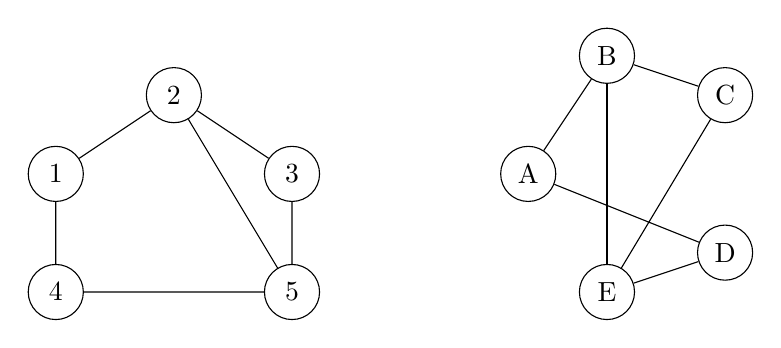
\begin{tikzpicture}[scale=1, every node/.style={circle,draw,minimum size=7mm,inner sep=0pt}]
% First graph (left)
\node (a1) at (0,0) {1};
\node (a2) at (1.5,1) {2};
\node (a3) at (3,0) {3};
\node (a4) at (0,-1.5) {4};
\node (a5) at (3,-1.5) {5};

\draw (a1) -- (a2) -- (a3) -- (a5) -- (a4) -- (a1);
\draw (a2) -- (a5);

% Second graph (right)
\node (b1) at (6,0) {A};
\node (b2) at (7,1.5) {B};
\node (b3) at (8.5,1) {C};
\node (b4) at (8.5,-1) {D};
\node (b5) at (7,-1.5) {E};

\draw (b1) -- (b2) -- (b3) -- (b5) -- (b4) -- (b1);
\draw (b2) -- (b5);
\end{tikzpicture}
\caption{Two isomorphic graphs on five vertices.}
\end{figure}

\begin{proposition}
Let $\varphi$ be an isomorphism from $X$ to $Y$. Then for every vertex $v \in V(X)$,
\[
\varphi\big(N_X(v)\big) = N_Y\big(\varphi(v)\big),
\]
where $N_X(v)$ denotes the set of neighbours of $v$ in $X$.
\end{proposition}

\begin{corollary}
\textcolor{blue}{Isomorphisms preserve degrees of vertices:} if $\varphi : X \to Y$ is an isomorphism, then
\[
\deg_X(v) = \deg_Y(\varphi(v)), \quad \forall v \in V(X).
\]
\end{corollary}
\begin{proof}
From the proposition, $\varphi$ gives a bijection between $N_X(v)$ and $N_Y(\varphi(v))$.  
Thus $|N_X(v)| = |N_Y(\varphi(v))|$, which means $\deg_X(v) = \deg_Y(\varphi(v))$.
\end{proof}
\section*{Graph Isomorphism Problem (GI Open Problem)}

\begin{itemize}
    \item \textbf{Problem:} Given two graphs, determine whether they are isomorphic, that is, structurally identical under some relabeling of vertices.
    \item Despite its simple statement, there is no efficient algorithm known to solve it in general.
    \item The current best algorithm is due to \textbf{L\'aszl\'o Babai (2015)}, which  uses group theory and graph automorphism groups to efficiently handle symmetries.
\end{itemize}

\subsection*{Special types of graphs}
A graph is \emph{complete} if every pair of distinct vertices is adjacent; the complete graph on $n$ vertices is denoted by $K_n$.  
A graph with vertices but no edges is called \emph{empty}.  
%The graph with no vertices and no edges is the \emph{null graph}. In this note we have always this assumption that $V(X) \neq \emptyset$
\begin{definition}
The \emph{complement} of a graph $X$, denoted $\overline{X}$, is the graph with the same vertex set as $X$ but with edge set
\[
E(\overline{X}) = \{\, xy : x,y \in V(X), x \neq y, \text{ and } xy \notin E(X) \,\}.
\]
That is, $\overline{X}$ contains exactly the edges not in $X$. 
\end{definition}

\begin{example}
If $X$ is the empty graph on 3 vertices (no edges), then $\overline{X} = K_3$, the complete graph on 3 vertices.
\end{example}

As we said our graphs   are simple graphs.  
A common generalisation is the \emph{directed graph} (or digraph), used to model asymmetric relationships.

\begin{definition}
A \emph{directed graph} $X$ consists of a vertex set $V(X)$ and an \emph{arc set} $A(X)$,  
where each arc is an ordered pair of distinct vertices.  
In diagrams, arcs are drawn as arrows from the first vertex to the second.
\end{definition}

\begin{figure}[h]
\centering
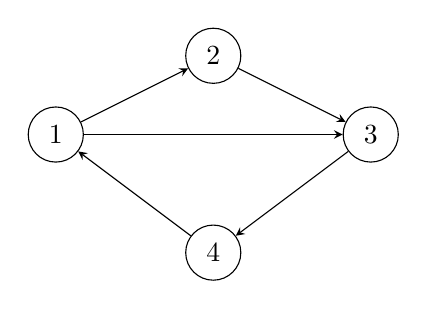
\begin{tikzpicture}[scale=1, every node/.style={circle,draw,minimum size=7mm,inner sep=0pt}, >=stealth]
\node (1) at (0,0) {1};
\node (2) at (2,1) {2};
\node (3) at (4,0) {3};
\node (4) at (2,-1.5) {4};

\draw[->] (1) -- (2);
\draw[->] (2) -- (3);
\draw[->] (3) -- (4);
\draw[->] (4) -- (1);
\draw[->] (1) -- (3);
\end{tikzpicture}
\caption{A directed graph.}
\end{figure}

Unless otherwise stated, all graphs in these notes are assumed to be finite, simple, and undirected.

\section{Subgraphs}

\begin{definition}
A \emph{subgraph} $Y$ of a graph $X$ is a graph with $V(Y) \subseteq V(X)$ and $E(Y) \subseteq E(X)$.
\end{definition}

If $V(Y) = V(X)$, then $Y$ is called a \emph{spanning subgraph} of $X$.  
Any spanning subgraph can be obtained by deleting edges from $X$.  
The number of spanning subgraphs of $X$ is $2^{|E(X)|}$.

\begin{definition}
An \emph{induced subgraph} of $X$ is a subgraph $Y$ where two vertices are adjacent in $Y$  
if and only if they are adjacent in $X$.  
Equivalently, it is obtained by deleting vertices from $X$ (and all incident edges).  
The number of induced subgraphs of $X$ is $2^{|V(X)|}$.
\end{definition}

\begin{figure}[h]
\centering

% Original graph
\begin{subfigure}[b]{0.3\textwidth}
\centering
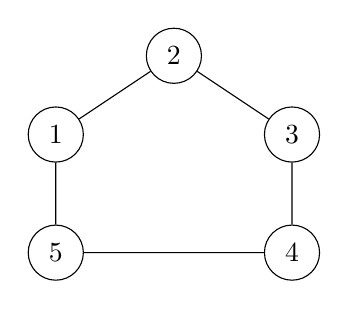
\begin{tikzpicture}[scale=1, every node/.style={circle,draw,minimum size=7mm,inner sep=0pt}]
\node (1) at (0,0) {1};
\node (2) at (1.5,1) {2};
\node (3) at (3,0) {3};
\node (4) at (3,-1.5) {4};
\node (5) at (0,-1.5) {5};

% Edges of 5-cycle
\draw (1) -- (2) -- (3) -- (4) -- (5) -- (1);

\end{tikzpicture}
\caption{Original graph}
\end{subfigure}
\hfill
% Spanning subgraph
\begin{subfigure}[b]{0.3\textwidth}
\centering
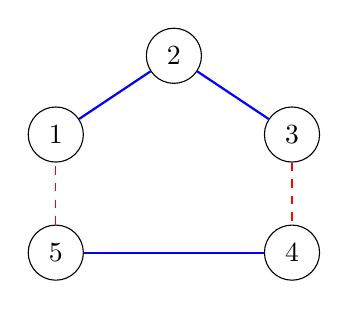
\begin{tikzpicture}[scale=1, every node/.style={circle,draw,minimum size=7mm,inner sep=0pt}]
\node (1) at (0,0) {1};
\node (2) at (1.5,1) {2};
\node (3) at (3,0) {3};
\node (4) at (3,-1.5) {4};
\node (5) at (0,-1.5) {5};

% Spanning subgraph edges (subset)
\draw[thick, blue] (1) -- (2);
\draw[thick, blue] (2) -- (3);
\draw[thick, blue] (4) -- (5);

% Removed edges shown dashed red for clarity (optional)
\draw[red, dashed] (3) -- (4);
\draw[red, dashed] (5) -- (1);

\end{tikzpicture}
\caption{Spanning subgraph}
\end{subfigure}
\hfill
% Induced subgraph
\begin{subfigure}[b]{0.3\textwidth}
\centering
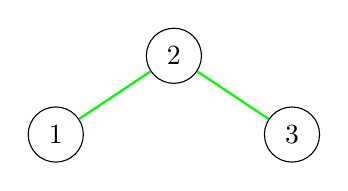
\begin{tikzpicture}[scale=1, every node/.style={circle,draw,minimum size=7mm,inner sep=0pt}]
\node (1) at (0,0) {1};
\node (2) at (1.5,1) {2};
\node (3) at (3,0) {3};

% Induced subgraph edges
\draw[thick, green] (1) -- (2) -- (3);

\end{tikzpicture}
\caption{Induced subgraph on \{1,2,3\}}
\end{subfigure}

\caption{Original graph, spanning subgraph, and induced subgraph on vertices \{1,2,3\}.}
\end{figure}



\subsection*{Special subgraphs}
A \emph{clique} is a complete subgraph; an \emph{independent set} is a set of vertices inducing no edges.  
The size of the largest clique in $X$ is the \emph{clique number} $\omega(X)$;  
the size of the largest independent set is the \emph{independence number} $\alpha(X)$.

\subsection*{Paths, connectivity, and cycles}
A \emph{path} of length $r$ from $x$ to $y$ is a sequence of $r+1$ distinct vertices beginning with $x$ and ending with $y$, such that consecutive vertices are adjacent.  
A graph is \textcolor{blue}{\emph{connected}} if there is a path between any two vertices; otherwise it is \emph{disconnected}.  
A \emph{component} of $X$ is a maximal connected induced subgraph.
\bigskip

\noindent\textbf{Exercise:} We have $\omega(X)=\alpha(\overline{X})$ and $\omega(\overline{X})=\alpha(X)$


\begin{example}
Consider the graph $X$ with vertex set $\{1,2,3,4,5,6\}$ and edges $\{12,23,45\}$.  
This graph has three components:
\[
\{1,2,3\} \quad \text{(connected by edges }12, 23\text{)},
\]
\[
\{4,5\} \quad \text{(connected by edge }45\text{)},
\]
\[
\{6\} \quad \text{(isolated vertex)}.
\]
\end{example}

\begin{center}
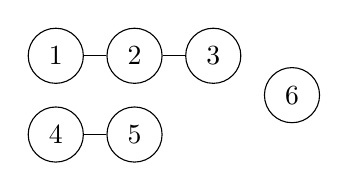
\begin{tikzpicture}[scale=1, every node/.style={circle,draw,minimum size=7mm,inner sep=0pt}]
  % Component 1: vertices 1,2,3 connected by edges 12, 23
  \node (1) at (0,1) {1};
  \node (2) at (1,1) {2};
  \node (3) at (2,1) {3};
  \draw (1) -- (2) -- (3);

  % Component 2: vertices 4,5 connected by edge 45
  \node (4) at (0,0) {4};
  \node (5) at (1,0) {5};
  \draw (4) -- (5);

  % Component 3: isolated vertex 6
  \node (6) at (3,0.5) {6};
\end{tikzpicture}
\end{center}

\bigskip
\begin{exercise}
Let $X$ be a simple graph with $n \ge 2$ vertices, and let $\overline{X}$ be its complement.

\begin{enumerate}
    \item Show that if $X$ is disconnected, then $\overline{X}$ is connected.
    \item Conclude that for any graph $X$ on $n \ge 2$ vertices, at least one of $X$ or $\overline{X}$ is connected.
    \item Give an example of a graph $X$ such that $X$ is disconnected but $\overline{X}$ is connected.
\end{enumerate}

\end{exercise}


\begin{theorem}
A graph $X$ is connected if and only if it has exactly one component.
\end{theorem}

\begin{proof}
By definition, the components are maximal connected induced subgraphs partitioning $V(X)$.  
If $X$ is connected, the whole graph is one maximal connected induced subgraph, so it has one component.  
Conversely, if there is only one component, $X$ itself is connected.
\end{proof}

\noindent\textcolor{blue}{A \emph{cycle}} is a connected graph in which every vertex has degree $2$.  
The smallest cycle is $K_3$. A graph in which each vertex has at least two neighbours must contain a cycle.

\noindent An \emph{acyclic} graph  is a graph with no cycles, it is also called a \emph{forest}.  A connected forest is called a \textcolor{blue}{\emph{tree}}. A \emph{spanning tree} is a spanning subgraph that is a tree.

\begin{theorem}
A graph has a spanning tree if and only if it is connected.
\end{theorem}

\begin{proof}
If a graph has a spanning tree, it is clearly connected.  
Conversely, if $X$ is connected, start with $X$ and repeatedly delete edges from cycles until no cycles remain;  
the resulting subgraph is connected and acyclic, hence a spanning tree.
\end{proof}

\begin{lemma}[Handshaking Lemma]
In any finite graph,
\[
\sum_{v \in V(X)} \deg(v) = 2|E(X)|.
\]
\end{lemma}
\begin{proof}
Each edge contributes exactly $2$ to the total degree count, one for each endpoint.  
Summing over all edges yields the formula.
\end{proof}

\bigskip\noindent\textbf{Exercise}
\begin{enumerate}
    \item Prove that a connected graph with maximum degree $\Delta(X) \le 2$ is either a path or a cycle.  
          In particular, if it is $2$-regular, it must be a cycle.
    \item Prove that any connected graph with minimum degree $\delta(X) \ge 2$ contains at least one cycle.
    \item Use the Handshaking Lemma to show that in any graph the number of vertices of odd degree is even.
    \item Prove that the number of spanning subgraphs of a graph $X$ is $2^{|E(X)|}$.
\end{enumerate}




\section*{Bipartite Graphs}

\begin{definition}
A graph $X$ is \emph{bipartite} if its vertex set $V(X)$ can be partitioned into two disjoint sets $U$ and $W$ such that every edge of $X$ connects a vertex in $U$ to a vertex in $W$.  
Equivalently, there are no edges between vertices within the same part.
\end{definition}

\begin{example}
The complete bipartite graph $K_{3,3}$ has vertex set partitioned into two sets of size 3 each, with every vertex in the first set connected to every vertex in the second set, and no edges within each set.

\begin{center}
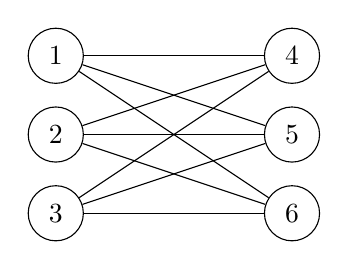
\begin{tikzpicture}[scale=1, every node/.style={circle,draw,minimum size=7mm,inner sep=0pt}]
  % Left set U
  \node (u1) at (0,2) {1};
  \node (u2) at (0,1) {2};
  \node (u3) at (0,0) {3};
  % Right set W
  \node (w1) at (3,2) {4};
  \node (w2) at (3,1) {5};
  \node (w3) at (3,0) {6};

  % Edges
  \foreach \u in {u1,u2,u3} {
    \foreach \w in {w1,w2,w3} {
      \draw (\u) -- (\w);
    }
  }
\end{tikzpicture}
\end{center}
\end{example}





\textbf{Definitions:}

1. Let $P$ be a path (or cycle) in a graph. The \emph{length} of $P$, denoted $|P|$, is the number of its edges. A cycle is called \emph{odd} (\emph{even}) if its length is odd (even).  


2. Let $X$ be a connected graph, and let $u,v$ be vertices of $X$. The \emph{distance} between $u$ and $v$, denoted $d_X(u,v)$, is defined by
\[
d_X(u,v) = \min \{ |P| \mid P \text{ is a path connecting } u \text{ and } v \}.
\]

\bigskip

\textbf{Exercise:} For any cycle, the number of vertices and the number of edges are equal.


\begin{theorem}
A graph is bipartite if and only if it contains no odd cycles.
\end{theorem}

\begin{proof}
\textbf{(Sketch)}

\textit{($\Rightarrow$)} Suppose $X$ is bipartite with parts $U$ and $W$.  
Any cycle must alternate vertices between $U$ and $W$.  
Thus, the cycle length must be even (since it must return to the starting vertex in the same part after an even number of steps).  
So $X$ contains no odd cycles.

\textit{($\Leftarrow$)} Suppose $X$ has no odd cycles.  
Pick any vertex $v$ and define:
\[
U = \{\,x \in V(X) : \text{the shortest path from } v \text{ to } x \text{ has even length}\,\}, 
\]
\[
W = \{\,x \in V(X) : \text{the shortest path from } v \text{ to } x \text{ has odd length}\,\}.
\]
If there were an edge within $U$ or within $W$, this would create an odd cycle (by combining the paths from $v$ to the two endpoints with that edge), contradicting the assumption.  
Therefore, $X$ is bipartite.
\end{proof}




\section{Automorphisms of Graphs}

An \emph{automorphism} of a graph \(X\) is an isomorphism from \(X\) to itself.  
In other words, it is a permutation of the vertex set \(V(X)\) that preserves adjacency: if \(x \sim y\) in \(X\), then \(g(x) \sim g(y)\) for an automorphism \(g\).

The set of all automorphisms of \(X\) forms a group under composition, called the \emph{automorphism group} of \(X\), denoted by \(\mathrm{Aut}(X)\).  
The identity permutation is the identity element of this group.  
If \(g \in \mathrm{Aut}(X)\), then its inverse \(g^{-1}\) is also in \(\mathrm{Aut}(X)\).

Since every automorphism is a permutation of \(V(X)\), \(\mathrm{Aut}(X)\) is a subgroup of the symmetric group \(\mathrm{Sym}(V(X))\).  
For a graph with \(n\) vertices, we write \(\mathrm{Sym}(n)\) for the full symmetric group.

\begin{example}
For the complete graph \(K_n\), every permutation of the vertices is an automorphism.  
Hence, \(\mathrm{Aut}(K_n) \cong \mathrm{Sym}(n)\).
\end{example}

If \(g \in \mathrm{Aut}(X)\) and \(Y\) is a subgraph of \(X\), define the image subgraph
\[
Y^g := (V(Y)^g, E(Y)^g) \quad \text{where} \quad V(Y)^g = \{g(v) : v \in V(Y)\}, \quad E(Y)^g = \{ \{g(u), g(v)\} : \{u,v\} \in E(Y) \}.
\]
Then \(Y^g\) is isomorphic to \(Y\) and is also a subgraph of \(X\).

\subsection*{Valency and Automorphisms}

The \emph{valency} (or degree) of a vertex \(x\) is the number of neighbors of \(x\).

\begin{lemma}
If \(g \in \mathrm{Aut}(X)\) and \(y = g(x)\), then \(x\) and \(y\) have the same valency.
\end{lemma}

\begin{proof}
Let \(N(x)\) be the subgraph induced by the neighbors of \(x\).  
Then
\[
N(x)^g = N(g(x)) = N(y).
\]
Since \(N(x)\) and \(N(y)\) are isomorphic subgraphs of \(X\), they have the same number of vertices, so \(x\) and \(y\) have the same valency.
\end{proof}

Thus, automorphisms permute vertices of equal valency among themselves.

A graph is called \emph{\(k\)-regular} if every vertex has valency \(k\).  
In particular, a \(3\)-regular graph is called \emph{cubic}, and a \(4\)-regular graph is sometimes called \emph{quartic}.

\subsection*{Distance and Automorphisms}

The \emph{distance} \(d(x,y)\) between vertices \(x\) and \(y\) is the length of a shortest path connecting them.

\begin{lemma}
If \(g \in \mathrm{Aut}(X)\), then for all vertices \(x,y\),
\[
d(x,y) = d(g(x), g(y)).
\]
\end{lemma}

\begin{proof}
Let \(P = (x = v_0, v_1, \ldots, v_k = y)\) be a shortest path from \(x\) to \(y\) of length \(k = d(x,y)\).  
Because \(g\) is an automorphism, it preserves adjacency, so the image path
\[
P^g = (g(v_0), g(v_1), \ldots, g(v_k))
\]
is a path of length \(k\) from \(g(x)\) to \(g(y)\).  
Thus,
\[
d(g(x), g(y)) \leq k = d(x,y).
\]

Similarly, applying \(g^{-1}\) shows
\[
d(x,y) = d(g^{-1}(g(x)), g^{-1}(g(y))) \leq d(g(x), g(y)).
\]

Combining these inequalities gives
\[
d(x,y) = d(g(x), g(y)),
\]
as required.
\end{proof}

\subsection*{Automorphisms of the Complement}

The \emph{complement} \(\overline{X}\) of a graph \(X\) has the same vertex set, where two vertices are adjacent in \(\overline{X}\) if and only if they are \emph{not} adjacent in \(X\).

\begin{lemma}
\[
\mathrm{Aut}(X) = \mathrm{Aut}(\overline{X}).
\]
\end{lemma}

\begin{proof}
Any automorphism preserves adjacency and non-adjacency, so it is also an automorphism of the complement.
\end{proof}

\subsection*{Examples of Automorphism Groups}

\textbf{Example}
Consider the graph \(G\) with vertex set
\[
V = \{1,2,3,4,5\}
\]
and edge set
\[
E = \{12, 13, 14, 25, 35\}.
\]

This graph resembles a star centered at vertex 1 with edges \(12, 13, 14\), plus edges \(25\) and \(35\) connecting vertices 2 and 3 to 5.

\[
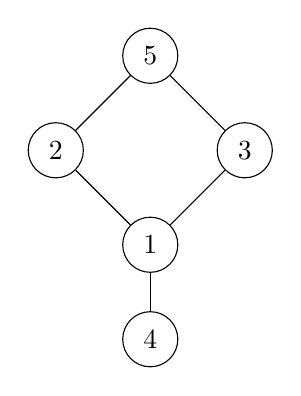
\begin{tikzpicture}[scale=1.2, every node/.style={circle,draw,minimum size=7mm,inner sep=0pt}]
\node (1) at (0,0) {1};
\node (2) at (-1,1) {2};
\node (3) at (1,1) {3};
\node (4) at (0,-1) {4};
\node (5) at (0,2) {5};

\draw (1) -- (2);
\draw (1) -- (3);
\draw (1) -- (4);
\draw (2) -- (5);
\draw (3) -- (5);
\end{tikzpicture}
\]

The degrees of the vertices are:
\[
\deg(1) = 3, \quad \deg(2) = 2, \quad \deg(3) = 2, \quad \deg(4) = 1, \quad \deg(5) = 2.
\]

Observe that vertices 2 and 3 share identical neighborhoods:
\[
N(2) = \{1,5\}, \quad N(3) = \{1,5\}.
\]

The mapping that swaps vertices 2 and 3 (and fixes all other vertices) preserves adjacency, as:
- edges \(12\) and \(13\) are swapped,
- edges \(25\) and \(35\) are swapped,
- vertices 1, 4, and 5 remain fixed.

Thus, the automorphism group of \(G\) consists of the identity and the transposition swapping 2 and 3, and so
\[
\mathrm{Aut}(G) \cong \mathbb{Z}_2.
\]




\begin{theorem}
For $n \geq 3$, the automorphism group of the cycle graph $C_n$ is isomorphic to the dihedral group $D_{2n}$:
\[
\mathrm{Aut}(C_n) \cong D_{2n}.
\]
\end{theorem}

\begin{proof}
Label the vertices of $C_n$ as
\[
V = \{ v_0, v_1, \dots, v_{n-1} \}
\]
with edges
\[
E = \{ \{v_i, v_{i+1 \pmod n}\} : i = 0, \dots, n-1 \}.
\]

If an automorphism of $C_n$ fixes two adjacent vertices, then it must be the identity. Indeed, if $\varphi(v_0) = v_0$ and $\varphi(v_1) = v_1$, then adjacency forces $\varphi(v_2) = v_2$, and inductively all vertices are fixed.

For $k = 0, \dots, n-1$, define the rotation
\[
\rho_k(v_i) = v_{i+k \pmod n},
\]
so that $\rho_k = (\rho_1)^k$ in particular. Also define the reflection
\[
\sigma(v_i) = v_{-i \pmod n}.
\]
The order of $\rho_1$ is $n$, since $(\rho_1)^n = \mathrm{id}$ and no smaller positive power is the identity. The order of $\sigma$ is $2$, since $\sigma^2 = \mathrm{id}$. Moreover,
\[
\sigma \rho_1 \sigma = \rho_1^{-1},
\]
as can be checked by
\[
\sigma \rho_1 \sigma (v_i) 
= \sigma \rho_1 (v_{-i}) 
= \sigma(v_{-i+1}) 
= v_{i-1} = \rho_1^{-1}(v_i).
\]

Let
\[
A = \langle \rho_1, \sigma \rangle.
\]
From the above relations, $A$ is isomorphic to the dihedral group $D_{2n}$ and has exactly $2n$ elements: the $n$ rotations $\rho_k$ and the $n$ reflections $\rho_k \sigma$. For each $i,j$, there exists $k$ with $\rho_k(v_i) = v_j$, namely $k \equiv j-i \pmod n$, so the rotations act transitively on $V$.

To show that $\mathrm{Aut}(C_n) \subseteq A$, let $\varphi \in \mathrm{Aut}(C_n)$. If $\varphi(v_0) = v_0$, then $\varphi$ sends $v_1$ to either $v_1$ or $v_{n-1}$. In the first case, by the initial observation, $\varphi = \mathrm{id}$. In the second case, $\varphi = \sigma$. Thus any automorphism fixing $v_0$ lies in $\{\mathrm{id}, \sigma\} \subset A$.

If instead $\varphi(v_0) = v_i$ for some $i$, choose $k$ such that $\rho_k(v_i) = v_0$. Then
\[
\psi := \rho_k \circ \varphi
\]
is an automorphism fixing $v_0$, hence $\psi \in \{\mathrm{id}, \sigma\} \subset A$. Therefore $\varphi = \rho_k^{-1} \psi \in A$.

Since $A \subseteq \mathrm{Aut}(C_n)$ by definition and we have shown $\mathrm{Aut}(C_n) \subseteq A$, it follows that
\[
\mathrm{Aut}(C_n) = A \cong D_{2n}.
\]
\end{proof}


\textbf{Example}[Path Graph \(P_n\)]
The path graph \(P_n\) has only two automorphisms: the identity and the "flip" reversing the path.  
Hence,
\[
\mathrm{Aut}(P_n) \cong \mathbb{Z}_2.
\]


\textbf{Example}[Complete Bipartite Graph \(K_{m,n}\)]
If \(m \neq n\), then
\[
\mathrm{Aut}(K_{m,n}) \cong S_m \times S_n,
\]
where \(S_m\) and \(S_n\) are the symmetric groups on the two parts.  
If \(m = n\), there is an additional automorphism swapping the two parts, so
\[
\mathrm{Aut}(K_{n,n}) \cong (S_n \times S_n) \rtimes \mathbb{Z}_2.
\]




\section{Johnson, Petersen and Kneser Graphs}

A particularly important family of graphs in algebraic and combinatorial graph theory are the \emph{$J(v,k,i)$ graphs}. They provide a natural way to translate problems about finite sets into graph theory.

\medskip
Let $v, k, i$ be integers with $v \ge k \ge i \ge 0$, and let $N$ be a fixed set of size $v$. The graph $J(v,k,i)$ is defined as follows:
\begin{itemize}
    \item The vertices are all $k$-element subsets of $N$.
    \item Two vertices (subsets) are adjacent if and only if their intersection has size $i$.
\end{itemize}
Thus, $J(v,k,i)$ has $\binom{v}{k}$ vertices and is a regular graph.

\bigskip\noindent\textbf{Exercise}
Show that $J(v,k,i)$ has $\binom{v}{k}$ vertices and is a $d$-regular graph, where
\[
d = \binom{k}{i} \binom{v-k}{k-i}.
\]


\medskip
A useful observation is that we may assume $v \ge 2k$:
\begin{lemma}
If $v \ge k \ge i$, then
\[
J(v,k,i) \cong J\big(v,\, v-k,\, v - 2k + i\big).
\]
\end{lemma}

\begin{proof}
Let $N$ be a fixed $v$-element set and $\binom{N}{k}$ be the set of all $k$-subsets of $N$ . Define a map
\[
\varphi: \binom{N}{k} \to \binom{N}{v-k}, \qquad \varphi(A) = N \setminus A.
\]
This map is clearly a bijection with inverse itself.

For any $k$-subsets $A,B \subseteq N$, we have
\[
\bigl|\varphi(A) \cap \varphi(B)\bigr| = |(N \setminus A) \cap (N \setminus B)| = |N \setminus (A \cup B)| = v - |A \cup B| = v - (|A|+|B|-|A \cap B|) = v - 2k + |A \cap B|.
\]

Hence, $|A \cap B| = i$ if and only if $\bigl|\varphi(A) \cap \varphi(B)\bigr| = v - 2k + i$. This shows that $\varphi$ preserves adjacency in the Johnson graphs, so it is an isomorphism
\[
J(v,k,i) \cong J\bigl(v,\,v-k,\,v-2k+i\bigr).
\]
\end{proof}


\medskip
When $v \ge 2k$, two special cases are of particular interest:
\begin{itemize}
    \item $J(v,k,k-1)$ — the \emph{Johnson graphs}.
    \item $J(v,k,0)$ — the \emph{Kneser graphs}.
\end{itemize}
The most famous example is the Kneser graph $J(5,2,0)$, which is the \emph{Petersen graph}.

\medskip
\noindent\textbf{Petersen Graph:}  
Vertices are the $2$-element subsets of $\{1,2,3,4,5\}$. Two vertices are adjacent if and only if they are disjoint as sets.

\begin{center}
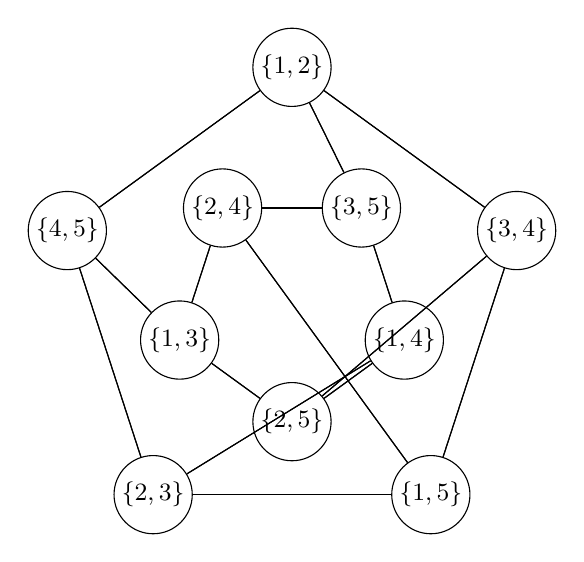
\begin{tikzpicture}[scale=3, every node/.style={circle,draw,fill=white,inner sep=1.5pt, font=\small}]
% --- Outer pentagon ---
\node (v12) at (90:1)   {$\{1,2\}$};
\node (v34) at (18:1)   {$\{3,4\}$};
\node (v15) at (306:1)  {$\{1,5\}$};
\node (v23) at (234:1)  {$\{2,3\}$};
\node (v45) at (162:1)  {$\{4,5\}$};

% --- Inner pentagram (rotated for symmetry) ---
\node (v35) at (54:0.5)   {$\{3,5\}$};
\node (v14) at (342:0.5)  {$\{1,4\}$};
\node (v25) at (270:0.5)  {$\{2,5\}$};
\node (v13) at (198:0.5)  {$\{1,3\}$};
\node (v24) at (126:0.5)  {$\{2,4\}$};

% --- Edges (disjoint subsets) ---
% {1,2}
\draw (v12) -- (v34);
\draw (v12) -- (v35);
\draw (v12) -- (v45);

% {3,4}
\draw (v34) -- (v15);
\draw (v34) -- (v25);
\draw (v34) -- (v12);

% {1,5}
\draw (v15) -- (v23);
\draw (v15) -- (v24);
\draw (v15) -- (v34);

% {2,3}
\draw (v23) -- (v14);
\draw (v23) -- (v45);
\draw (v23) -- (v15);

% {4,5}
\draw (v45) -- (v12);
\draw (v45) -- (v13);
\draw (v45) -- (v23);

% {3,5}
\draw (v35) -- (v12);
\draw (v35) -- (v14);
\draw (v35) -- (v24);

% {1,4}
\draw (v14) -- (v23);
\draw (v14) -- (v25);
\draw (v14) -- (v35);

% {2,5}
\draw (v25) -- (v14);
\draw (v25) -- (v34);
\draw (v25) -- (v13);

% {1,3}
\draw (v13) -- (v24);
\draw (v13) -- (v25);
\draw (v13) -- (v45);

% {2,4}
\draw (v24) -- (v13);
\draw (v24) -- (v15);
\draw (v24) -- (v35);

\end{tikzpicture}
\end{center}

\begin{figure}[htbp]
    \centering
    \includegraphics[width=0.6\textwidth]{Petersengraph.png}
    \caption{The Petersen graph, labeled by 2-element subsets of $[5]$.}
    \label{fig:petersen}
\end{figure}


The Petersen graph is $3$-regular, has $10$ vertices and $15$ edges, and plays a central role in many areas of graph theory.

\medskip
\noindent\textbf{Automorphisms.}  
If $g$ is a permutation of $N$ and $S \subseteq N$, define
\[
S^g = \{\, s^g : s \in S \,\}.
\]
Each such $g$ induces a permutation of the vertices of $J(v,k,i)$, and if $|S \cap T| = i$ then $|S^g \cap T^g| = i$, so $g$ is an automorphism of $J(v,k,i)$. Thus:

\begin{lemma}
For $v \ge k \ge i$, $\mathrm{Aut}(J(v,k,i))$ contains a subgroup isomorphic to $\mathrm{Sym}(v)$.
\end{lemma}
\bigskip

\noindent In fact, in most cases $\mathrm{Aut}(J(v,k,i)) \cong \mathrm{Sym}(v)$, though proving this can be nontrivial. In particular, for the \emph{Kneser graph} $K(v,k,0)$  in many cases we have 
\[
\mathrm{Aut}(K(v,k,0)) \cong \mathrm{Sym}(v) \quad \text{for } v \ge 2k+1.
\]

\bigskip

\noindent\textbf{Open Problem:} Determine all triples $(v,k,i)$ for which
\[
\mathrm{Aut}(J(v,k,i)) \cong \mathrm{Sym}(v).
\]
\bigskip

That is, classify the parameters for which the automorphism group of a Johnson graph (or its Kneser graph special case) is isomorphic to the full symmetric group on $v$ vertices.

\bigskip


\begin{theorem}
The automorphism group of the Petersen graph \(P\) is isomorphic to \(S_5\) in its natural action on the 2-subsets of \([5] = \{1,2,3,4,5\}\).
\end{theorem}

\begin{proof}
We label the vertices of \(P\) by the 2-element subsets of \([5]\), with two vertices adjacent if and only if the corresponding subsets are disjoint.  

---

\textbf{Step 1: Structure of the Petersen graph in this labeling.}  
The vertices can be divided into two 5-cycles:
\begin{itemize}
    \item The \emph{outer 5-cycle}, consisting of vertices
    \[
    12,\; 34,\; 15,\; 23,\; 45,
    \]
    where edges follow the cycle in that order (each consecutive pair is disjoint).
    \item The \emph{inner 5-cycle}, consisting of the remaining 2-subsets
    \[
    13,\; 24,\; 35,\; 14,\; 25,
    \]
    again forming a 5-cycle in that cyclic order.
\end{itemize}

---

\textbf{Step 2: Independent sets of maximum size.}  
In any graph, an automorphism sends independent sets to independent sets of the same size. In a 5-cycle, the largest independent set has size 2. Since \(P\) consists of two 5-cycles connected in a specific way, a maximum independent set in \(P\) can contain at most two vertices from the outer cycle and at most two from the inner cycle. Hence:
\[
\alpha(P) = 4,
\]
and every maximum independent set has exactly two vertices from each cycle.

A simple example of a size-4 independent set is:
\[
I_j := \{\text{all 2-subsets of } [5] \text{ containing } j\}.
\]
For example:
\[
I_1 = \{12, 13, 14, 15\}.
\]
Clearly, there are exactly 5 such sets \(I_1, I_2, I_3, I_4, I_5\), one for each element of \([5]\).

---

\textbf{Step 3: Classification of all maximum independent sets.}  
Let \(I\) be any independent set of size 4 in \(P\). By Step 1, it must contain exactly two vertices from the outer cycle and two from the inner cycle.  

The outer 5-cycle has a rotation symmetry given by the permutation
\[
\rho = (1\,5\,3\,2\,4) \in S_5,
\]
which acts on the 2-subset labels of \(P\). By applying an automorphism corresponding to a rotation of the outer cycle, we can assume without loss of generality that:
\[
\text{Outer vertices in } I: \quad 34 \ \text{and} \ 45.
\]

Looking at the adjacency structure of \(P\), the only way to complete \(I\) to an independent set of size 4 is to take the inner vertices:
\[
14 \ \text{and} \ 24.
\]
This set is exactly \(I_4\).

Hence, every maximum independent set is of the form \(I_j\) for some \(j \in [5]\).

---

\textbf{Step 4: Action of \(\mathrm{Aut}(P)\) on the family \(\{I_j\}\).}  
We have shown that the family of maximum independent sets is:
\[
\mathcal{I} = \{I_1, I_2, I_3, I_4, I_5\}.
\]
Any automorphism of \(P\) permutes these sets, giving a homomorphism:
\[
\varphi: \mathrm{Aut}(P) \to S_5.
\]
This map is surjective because the action of \(S_5\) on the underlying 2-subset labeling of \(P\) preserves adjacency, so \(S_5 \subseteq \mathrm{Aut}(P)\).

---

\textbf{Step 5: Kernel of \(\varphi\).}  
Suppose \(g \in \mathrm{Aut}(P)\) fixes each \(I_j\) setwise. Then for any distinct \(j,k\), the intersection
\[
I_j \cap I_k = \{\{j,k\}\}
\]
is a single vertex of \(P\), so \(g\) must fix this vertex. Since this holds for all pairs \(j,k\), \(g\) fixes every vertex of \(P\), hence \(g\) is the identity. Therefore:
\[
\ker(\varphi) = \{ \mathrm{id} \}.
\]

---

\textbf{Step 6: Conclusion.}  
Since \(\varphi\) is an injective homomorphism from \(\mathrm{Aut}(P)\) into \(S_5\) and we already have \(S_5 \subseteq \mathrm{Aut}(P)\), it follows that:
\[
\mathrm{Aut}(P) \cong S_5.
\]
\end{proof}

\subsection*{ Levi Graphs}


\noindent An \emph{incidence structure} is a pair $(P, \mathcal{B})$, where 
\begin{itemize}
    \item $P$ is a set of \emph{points}, and
    \item $\mathcal{B}$ is a set of \emph{blocks} (also called \emph{lines}),
\end{itemize}
together with an incidence relation indicating which points lie in which blocks.  

\bigskip

\noindent The \emph{Levi graph} (or \emph{incidence graph}) of an incidence structure $(P, \mathcal{B})$ is the bipartite graph with vertex set $P \cup \mathcal{B}$, where a point $p \in P$ is adjacent to a block $B \in \mathcal{B}$ if and only if $p$ is incident with $B$ (i.e., $p \in B$).



\begin{definition}
\begin{enumerate}

A \emph{polarity} of an incidence structure $(P, \mathcal{B})$ is a bijection 
\[
\pi: P \cup \mathcal{B} \to P \cup \mathcal{B}
\] 
satisfying the following properties:
\begin{enumerate}
    \item $\pi$ maps points to lines and lines to points,
    \item $\pi$ is an involution: $\pi^2$ is the identity, and
    \item incidence is preserved in the sense that for any point $p \in P$ and line $\ell \in \mathcal{B}$, 
    \[
    p \in \ell \quad \Longleftrightarrow \quad \pi(\ell) \in \pi(p).
    \]
\end{enumerate}
\end{enumerate}
\end{definition}
\bigskip


\noindent A configuration is \emph{self-dual} if it admits a polarity. In other words, points and lines can be interchanged while preserving the incidence structure.
\bigskip

\noindent\textbf{Remarks:} A Levi graphs is  bipartite, so Petersen graph is not a Levi graph.
\bigskip

In what follows, we present some classical examples of Levi graphs such as:

\begin{itemize}
\item The \emph{Tutte–Coxeter graph}.
    \item The \emph{Heawood graph} which is the  Levi graph of the Fano plane (self-dual configuration with 7 points and 7 lines). 
    %\item The \emph{Hoffman–Singleton graph}: Levi graph of a certain $(7,5)$-configuration related to the pentagon–heptad structure.
    
    %\item The \emph{Petersen graph} is \emph{not} a Levi graph, but it can be constructed from 2-element subsets of a 5-element set with adjacency given by disjointness.
\end{itemize}




\section{The Tutte--Coxeter Graph (Tutte 8-cage)}

\begin{definition}[Tutte--Coxeter Graph]
Let $\Omega=\{1,2,3,4,5,6\}$.
\begin{itemize}
  \item A \emph{duad} is a $2$-element subset of $\Omega$. Denote the set of duads by
  \[
    D=\bigl\{\{i,j\}\subset \Omega : i<j \bigr\}, \quad |D|=15.
  \]
  \item A \emph{syntheme} is a partition of $\Omega$ into three disjoint duads. Denote the set of synthemes by $S$, so $|S|=15$.
\end{itemize}
The \emph{Tutte--Coxeter graph} $\Gamma$ is the bipartite incidence graph with parts $D$ and $S$, where $d\in D$ is adjacent to $s\in S$ if and only if $d\in s$.
\end{definition}

\begin{theorem}
The automorphism group of the Tutte--Coxeter graph is
\[
  \operatorname{Aut}(\Gamma) \;\cong\; \operatorname{Aut}(S_6) \;\cong\; S_6 \rtimes C_2,
\]
and hence has order $1440$.
\end{theorem}

\begin{proof}
\textbf{Step 1. Side-preserving automorphisms.}
Any $\sigma \in S_6$ permutes the symbols of $\Omega$, thereby permuting duads and synthemes and preserving incidence. Thus
\[
  S_6 \leq \operatorname{Aut}(\Gamma).
\]

To see there are no additional side-preserving automorphisms, observe that from the graph $\Gamma$ alone we can reconstruct the six symbols of $\Omega$.  
For duads $a,b\in D$ define
\[
  R(a,b) = \#\{\, s\in S : a\sim s \sim b \,\}.
\]
A simple check shows:
\[
  R(a,b) = 
  \begin{cases}
    3 & a=b,\\
    0 & a\neq b \text{ and } a\cap b\neq \varnothing,\\
    1 & a\cap b=\varnothing.
  \end{cases}
\]
Thus we can recognize within $\Gamma$ when two duads intersect.  
Construct a graph $X$ on $D$ where $a,b$ are adjacent iff $a\cap b\neq \varnothing$.  
Then for each $i\in \Omega$, the five duads containing $i$ form a clique $K_5$ in $X$, and these six cliques are exactly the maximal $5$-cliques in $X$. Hence the six symbols of $\Omega$ are canonically identifiable from $\Gamma$.

Therefore every automorphism of $\Gamma$ preserving the bipartition induces a permutation of the six cliques, i.e.\ an element of $S_6$. This proves
\[
  \operatorname{Aut}^+(\Gamma) \cong S_6.
\]

\textbf{Step 2. Existence of a side-swapping automorphism.}
\medskip
\noindent
We can show that the incidence structure \((D,S)\) is \emph{self-dual}. 
However, the proof requires some group-theoretic machinery, in particular 
the existence of the exceptional outer automorphism of the symmetric group \(S_6\). 
We leave this as an exercise, but we include below a brief sketch as a proposition.

\medskip
\noindent
In fact, there exists a polarity \(\pi\) interchanging duads and synthemes 
while preserving incidence:
\[
d \in s \quad \Longleftrightarrow \quad \pi(s) \in \pi(d).
\]
This polarity induces a graph automorphism \(\tau\) of the Tutte--Coxeter graph 
satisfying
\[
\tau(D) = S, \qquad \tau(S) = D,
\]
showing that the graph is self-dual.

\textbf{Step 3. Conclusion.}
Thus
\[
  \operatorname{Aut}(\Gamma) = \langle \operatorname{Aut}^+(\Gamma), \tau\rangle \cong S_6 \rtimes C_2.
\]
It is well known that $S_6$ has a unique nontrivial outer automorphism, and adjoining $\tau$ realizes this extension. Therefore
\[
  |\operatorname{Aut}(\Gamma)| = 2\cdot |S_6| = 2\cdot 720 = 1440,
\]
as claimed.
\end{proof}

\medskip
\begin{proposition}
Let \(\Omega=\{1,2,3,4,5,6\}\), let \(D\) be the set of duads (2-subsets of \(\Omega\)) and let \(S\) be the set of synthemes (partitions of \(\Omega\) into three disjoint duads).  
Then there exists a bijection \(f\!:D\to S\) which is a polarity of the duad–syntheme incidence structure; that is,
\[
d\in s \quad\Longleftrightarrow\quad f(s)\in f(d)
\]
for all \(d\in D\), \(s\in S\), and \(f^2=\mathrm{id}\). Consequently the Tutte--Coxeter Levi graph is self-dual.
\end{proposition}
\begin{proof}
\textbf{(1) ( see the book of Rotman, corollary 7.6) The outer automorphism \(\sigma\) and its effect on cycle types.}  
It is a classical fact that \(S_6\) admits a nontrivial outer automorphism
\(\sigma:S_6\to S_6\). One convenient way to view \(\sigma\) is by its action on conjugacy classes: under \(\sigma\) a transposition (cycle type \(2\)) is sent to a product of three disjoint transpositions (cycle type \(2^3\)), and conversely, a product of three disjoint transpositions is sent to a transposition. (Any concrete model of the outer automorphism — e.g. via \( \mathrm{PGL}_2(5)\) or via complementary 3-sets — gives this behavior.)

\medskip
\textbf{(2) Identifying duads and synthemes with permutations.}  
Associate to each duad \(d=\{a,b\}\in D\) the transposition \((ab)\in S_6\).  
Associate to each syntheme \(s\in S\) the permutation \(\tau_s\in S_6\) which is the product of the three disjoint transpositions that form \(s\). Thus incidence \(d\in s\) is equivalent to the transposition \((ab)\) being one of the three disjoint transpositions whose product is \(\tau_s\).

\medskip
\textbf{(3) Define \(f\colon D\to S\) via \(\sigma\).}  
For a duad \(d=\{a,b\}\) let \(t_d=(ab)\). Consider \(\sigma(t_d)\). By (1), \(\sigma(t_d)\) is a permutation of cycle type \(2^3\); its three transposition factors correspond to a unique syntheme \(s\in S\). Define \(f(d)=s\). This produces a map \(f\colon D\to S\).

\medskip
\textbf{(4) Well-definedness and bijectivity.}  
If \(t_{d_1}=t_{d_2}\) then \(d_1=d_2\), so the assignment is well defined. The map \(f\) is injective because \(\sigma\) is injective and different transpositions land in different \(2^3\)-type elements (so give different synthemes). Since \(|D|=|S|=15\), injectivity implies bijectivity.

\medskip
\textbf{(5) Incidence is reversed by \(f\).}  
Fix \(d=\{a,b\}\in D\) and \(s\in S\). Let \(t_d=(ab)\) and let \(\tau_s\) be the product of the three transpositions in \(s\). Then
\[
d\in s \quad\Longleftrightarrow\quad t_d \text{ is one of the three transpositions whose product is }\tau_s.
\]
Apply \(\sigma\) to both sides. Using that \(\sigma\) is a homomorphism of the group structure (though outer, it still permutes conjugacy classes and respects products up to group law), we obtain that \( \sigma(t_d)\) is one of the three transpositions in the product \(\sigma(\tau_s)\). By the definition of \(f\),
\[
\sigma(t_d)\ \text{corresponds to the syntheme } f(d),\qquad
\sigma(\tau_s)\ \text{corresponds to the duad } f(s).
\]
Thus
\[
t_d \text{ appears in } \tau_s \quad\Longleftrightarrow\quad \sigma(\tau_s)\ \text{contains a transposition appearing in }\sigma(t_d),
\]
which translates exactly to
\[
d\in s \quad\Longleftrightarrow\quad f(s)\in f(d).
\]
Therefore \(f\) reverses incidence as required for a polarity.

\medskip
\textbf{(6) Making \(f\) involutory.}  
The map \(\sigma\) represents a nontrivial element of \(\mathrm{Out}(S_6)\), and a standard fact is \(\sigma^2\) is inner: there exists \(h\in S_6\) with \(\sigma^2=\operatorname{conj}_h\) (conjugation by \(h\)). For the bijection \(f\) constructed above we then have, for every \(d\in D\),
\[
f(f(d)) = \text{(syntheme corresponding to }\sigma(\text{product corresponding to }f(d))\text{)}.
\]
One checks (using \(\sigma^2=\operatorname{conj}_h\)) that \(f^2\) acts on \(D\) as the permutation induced by \(h\). Thus \(f^2\) is an inner permutation of the duads. Replacing \(f\) by the modified map \(d\mapsto h^{-1}\cdot f(d)\) (equivalently composing \(f\) with the involutive action of \(h^{-1}\)) yields a new bijection \(\tilde f\) which still intertwines the two \(S_6\)-actions but satisfies \(\tilde f^2=\mathrm{id}\). Therefore we obtain a polarity that is an involution.

\medskip
\textbf{Conclusion.} The bijection \(f\) (after the adjustment above if desired) is an incidence-reversing involution \(D\leftrightarrow S\); i.e. a polarity of the duad–syntheme incidence structure. Hence the Tutte--Coxeter Levi graph is self-dual.
\end{proof}

\bigskip

\noindent
The \emph{girth} of a graph \(X\), denoted by \(\mathrm{girth}(X)\), 
is the length of the shortest cycle in \(X\).
If \(X\) has no cycles (that is, \(X\) is acyclic), we set \(\mathrm{girth}(X)=\infty\).

\medskip
\noindent
The \emph{diameter} of a connected graph \(X\), denoted by \(\mathrm{diam}(X)\), 
is the maximum distance between any two vertices of \(X\); that is,
\[
\mathrm{diam}(X) = \max_{u,v \in V(X)} d_X(u,v),
\]
where \(d_X(u,v)\) is the length of the shortest path between \(u\) and \(v\).


\bigskip
\noindent\textbf{Exercise 1.} 
Show that the Johnson graph $J(v,k,i)$ has 
\[
\binom{v}{k} 
\] 
vertices and is $d$-regular, where
\[
d = \binom{k}{i} \binom{v-k}{k-i}.
\]

\bigskip
\noindent\textbf{Exercise 2.} 
Show that  the Petersen graph $P$  is connected and has diameter 3 and girth 5.


\section*{Girth $8$ and diameter $4$ of the Tutte--Coxeter graph}


%The incidence structure $(D,S,I)$ satisfies the axioms of a generalized quadrangle of order $(2,2)$ (often denoted $GQ(2,2)$): every point (duad) lies on exactly $3$ lines (synthemes), every line contains exactly $3$ points, and for any point $x$ and line $\ell$ not incident with $x$ there is a unique point on $\ell$ collinear with $x$.  The well-known combinatorial consequence of these axioms is that the Levi graph of a generalized quadrangle has girth $8$ and diameter $4$.  We prove these two facts directly for $\Gamma$.

\begin{theorem}
The Tutte--Coxeter graph $\Gamma$ has girth $8$ and diameter $4$.
\end{theorem}

\begin{proof}
We treat girth and diameter separately.

\medskip\noindent\textbf{(1) Girth is $8$.}

Since $\Gamma$ is bipartite any cycle has even length; so the possible cycle lengths are $4,6,8,\dots$.
We show no $4$- or $6$-cycle can occur; hence the shortest possible cycle is length $8$.

\emph{No $4$-cycles.}  Suppose there were a $4$-cycle
\[
d_1 - s_1 - d_2 - s_2 - d_1,
\]
with $d_i\in D$ and $s_j\in S$. Then both synthemes $s_1$ and $s_2$ contain the two duads $d_1$ and $d_2$.  But by construction of synthemes, two distinct duads determine at most one syntheme containing both. Therefore $\Gamma$ has no $4$-cycle.

\emph{No $6$-cycles.}  Suppose there were a $6$-cycle
\[
d_1 - s_1 - d_2 - s_2 - d_3 - s_3 - d_1 .
\]
Interpret this in the incidence structure: $d_i\in s_{i}$ and $d_{i+1}\in s_{i}$ (indices mod \(3\)).  Pick the syntheme $s_1$ and the point (duad) $d_3$ not on $s_1$; then we should have a unique point on $s_1$ which is in a same syntheme with $d_3$ (collinear). But in the supposed $6$-cycle both $d_1$ and $d_2$ are points of $s_1$ that are collinear with $d_3$ (since the cycle gives paths $d_3-s_3-d_1$ and $d_3-s_2-d_2$), contradicting uniqueness. Hence no $6$-cycle exists.

With $4$- and $6$-cycles excluded, the smallest possible even cycle length is $8$ and we can see that there is 8-cycle.

\medskip\noindent\textbf{(2) Diameter is $4$.}

Let $x,y$ be arbitrary vertices of $\Gamma$. We must show there is a path of length at most $4$ joining $x$ to $y$. Since $\Gamma$ is bipartite, distances between vertices in the same part are even and between opposite parts are odd; it therefore suffices to show that any two vertices of the same part are at graph-distance at most $4$ (this will imply the worst-case distance between arbitrary vertices is at most $4$).

We consider two cases.

\emph{Case A: $x,y$ are in different parts.} Then either $x$ is adjacent to $y$ (distance $1$), or else there exists a neighbor $z$ of $x$ that is adjacent to $y$ giving a path of length $3$ at most. In fact if $x$ is a duad and $y$ a syntheme not incident to $x$, take any syntheme through $x$;  there is a unique duad on that syntheme collinear with $y$, and that furnishes a path of length $3$. Thus distance between opposite parts is at most $3$.

\emph{Case B: $x,y$ lie in the same part.} Without loss of generality assume $x,y\in D$ (duads). If $x$ and $y$ are both contained in a common syntheme then $\operatorname{dist}(x,y)=2$. Otherwise they are not collinear in the incidence structure; pick any syntheme $s$ incident with $x$. Then there is a unique duad $z\in s$ which is collinear with $y$. Hence we have the path
\[
x - s - z - s' - y,
\]
where \(s'\) is some syntheme containing both \(z\) and \(y\) (such \(s'\) exists because \(z\) and \(y\) are collinear). This is a path of length \(4\) from \(x\) to \(y\). Thus any two duads are at distance at most \(4\). The same argument applies when $x,y\in S$ (synthemes): if two synthemes are not adjacent, pick a duad on one and then we can  find the unique duad to approach the other; this produces a length-$4$ path.

Combining the two cases we see every pair of vertices is at distance $\le 4$, while examples of vertex pairs at distance exactly $4$ exist (e.g. certain pairs of duads that intersect), so the diameter is exactly $4$.

\medskip

Therefore the Tutte--Coxeter graph $\Gamma$ has girth $8$ and diameter $4$, as required.
\end{proof}
\begin{figure}[h!]
\centering
\includegraphics[width=0.6\textwidth]{TutteCoxeterGraph.pdf}
\caption{The Tutte–Coxeter graph.}
\label{fig:TutteCoxeter}
\end{figure}




\section{The Fano Plane and the Coxeter Graph}


The \textbf{Fano plane} is the unique projective plane of order 2. It is the smallest non-trivial example of a projective plane and is denoted $\mathrm{PG}(2,2)$, representing the 2-dimensional projective space over the finite field $\mathbb{F}_2$.

Formally, it is an incidence structure $(\mathcal{P}, \mathcal{L})$ where:
\begin{itemize}
    \item $\mathcal{P} = \{1, 2, 3, 4, 5, 6, 7\}$ is a set of \textbf{7 points}.
    \item $\mathcal{L}$ is a collection of \textbf{7 lines}, each a 3-element subset of $\mathcal{P}$.
\end{itemize}

The incidence relation must satisfy the following axioms:
\begin{enumerate}[label=(\roman*)]
    \item Any two distinct points lie on exactly one line.
    \item Any two distinct lines intersect in exactly one point.
    \item Each line contains exactly 3 points, and through each point pass exactly 3 lines.
\end{enumerate}

A standard labeling satisfying these axioms is:
\[
\mathcal{L} = \{
\{1,2,3\},\
\{1,4,5\},\
\{1,6,7\},\
\{2,4,6\},\
\{2,5,7\},\
\{3,4,7\},\
\{3,5,6\}
\}.
\]

This structure can be visually represented by a diagram where points are dots and lines are smooth curves (often circles), with each line containing three points.

\subsection*{Vector Space Construction}

A more algebraic construction reveals the source of its symmetry. Consider the 3-dimensional vector space $V = \mathbb{F}_2^3$ over the field $\mathbb{F}_2 = \{0, 1\}$.
\begin{itemize}
    \item The \textbf{points} of the Fano plane are the 1-dimensional subspaces of $V$. Since $\mathbb{F}_2$ has only one nonzero element, each 1-dimensional subspace contains exactly one nonzero vector. There are $(2^3 - 1) = 7$ such vectors, so $|\mathcal{P}| = 7$.
    \item The \textbf{lines} are the 2-dimensional subspaces of $V$. A 2-dimensional subspace contains $(2^2 - 1) = 3$ nonzero vectors, which are exactly the three nonzero vectors of the two 1-dimensional subspaces it contains. This explains why each line has 3 points.
    \item \textbf{Incidence} is defined by containment: a point (1-subspace) lies on a line (2-subspace) if and only if the 1-subspace is contained in the 2-subspace.
\end{itemize}

This construction directly implies that the automorphisms of the Fano plane are induced by the linear symmetries of $V$.

\subsection*{Automorphism Group}

An \textbf{automorphism} (or \textbf{collineation}) of the Fano plane is a permutation $\sigma : \mathcal{P} \to \mathcal{P}$ that maps lines to lines, i.e., for every $\ell \in \mathcal{L}$, $\sigma(\ell) \in \mathcal{L}$ and  that preserves incidence; that is,
for every point $p \in \mathcal{P}$ and line $\ell \in \mathcal{L}$,
\[
p \in \ell \quad \Longleftrightarrow \quad \sigma(p) \in \sigma(\ell).
\]

\begin{theorem}
$\operatorname{Aut}(\mathcal{P}, \mathcal{L}) \cong \mathrm{PGL}(3,2)$.
\end{theorem}

\begin{proof}
\begin{itemize}
    \item Every invertible linear map $A \in \mathrm{GL}(3,2)$ permutes the 1-dimensional and 2-dimensional subspaces of $V$, thus inducing a collineation.
   
    \item The order of $\mathrm{GL}(3,2)$ is calculated by counting ordered bases for $\mathbb{F}_2^3$:
    \[
    |\mathrm{GL}(3,2)| = (2^3 - 1)(2^3 - 2)(2^3 - 2^2) = 7 \cdot 6 \cdot 4 = 168.
    \]
    \item It is a classical result that $\mathrm{GL}(3,2) \cong \mathrm{PSL}(2,7)$.
    \item Furthermore,by the Fundamental Theorem of Projective Geometry, every collineation arises from a linear map, so the group is exactly $\mathrm{PGL}(3,2)$.
\end{itemize}
Thus, the automorphism group of the Fano plane is a simple group of order \textbf{168}.
\end{proof}

\begin{figure}[h]
    \centering
    \includegraphics[width=0.4\textwidth]{fanoplane.png} % adjust filename and width
    \caption{The Fano plane.}
\end{figure}





\subsection*{The Coxeter Graph}



The \textbf{Coxeter graph} is a famous 3-regular (cubic) graph with 28 vertices and 42 edges. It is known for its high symmetry and interesting properties. 

%\subsubsection*{Construction A: Via Anti-Flags}

%\begin{itemize}
   % \item Let $(\mathcal P, \mathcal L)$ be the Fano plane (7 points, 7 lines). An \textbf{anti-flag} is a pair $(p,\ell)$ where $p \in \mathcal P$ is \emph{not} on the line $\ell \in \mathcal L$. 

    %\item There are $7$ choices for $p$ and, for each $p$, $4$ lines $\ell$ not containing $p$, so there are $7\times 4 = 28$ anti-flags. These will be the vertices of the Coxeter graph $\Gamma$.

   % \item Two vertices $(p_1,\ell_1)$ and $(p_2,\ell_2)$ are adjacent if and only if
   % \[
   % p_1 \in \ell_2 \quad \text{and} \quad p_2 \in \ell_1.
   % \]
   % This defines a cubic graph on 28 vertices — the Coxeter graph.
    
   % \item This construction is naturally symmetric: any collineation (automorphism) of the Fano plane sends anti-flags to anti-flags and preserves adjacency. Hence
   % \[
   % \operatorname{Aut}(\text{Fano plane}) \cong \mathrm{PSL}(2,7)
    %\]
   % acts faithfully on $\Gamma$.

    %\item Furthermore, the \emph{outer automorphism} of $\mathrm{PSL}(2,7)$, realized as the full $\mathrm{PGL}(2,7)$, corresponds to the point-line duality of the Fano plane (swapping points and lines). In terms of anti-flags, this still produces automorphisms of $\Gamma$, doubling the size of the automorphism group.

   % \item Therefore,
   % \[
   % \operatorname{Aut}(\Gamma) \geq \mathrm{PGL}(2,7), \quad |\operatorname{Aut}(\Gamma)|\geq 336.
%    \]

    %\item The embedding is now clear: each automorphism of $\Gamma$ is induced by a permutation of the 7 points and 7 lines of the Fano plane that preserves incidence (or dual incidence), so $\operatorname{Aut}(\Gamma)$ naturally sits inside $S_7 \wr C_2 \subseteq S_{14}$ if you consider points and lines together, or inside $S_8$ if you realize it via the 8-point construction $X = \mathbb{P}^1(\mathbb{F}_7)$ as before.
%\end{itemize}


\subsubsection*{Construction As an Induced Subgraph of $K(7,3)$}

This construction is crucial for understanding the graph's automorphisms.
\begin{itemize}
    \item Let $K(7,3)$ be the \textbf{Kneser graph} whose vertices are all 3-element subsets of a 7-element set $\mathcal{P}$ (the points of the Fano plane). Two vertices are adjacent if their corresponding subsets are disjoint. $K(7,3)$ has $\binom{7}{3}=35$ vertices.
    \item Let $\mathcal{L}$ be the set of 7 subsets that are lines of the Fano plane. It is a set of 7 triples that Each pair of them has exactly one point in common.
    \item Let $\mathcal{T} = \binom{\mathcal{P}}{3} \setminus \mathcal{L}$ be the set of 28 remaining 3-element subsets.
    \item The \textbf{Coxeter graph $\Gamma$} is defined as the \textbf{induced subgraph} of $K(7,3)$ on the vertex set $\mathcal{T}$. Two vertices in $\Gamma$ are adjacent if and only if their corresponding triples are disjoint.
\end{itemize}

%\subsection*{Equivalence of the Two Constructions of the Coxeter Graph}

%We now show that the two descriptions of the Coxeter graph are equivalent:
%egin{enumerate}
   % \item the \textbf{anti-flag construction}, whose vertices are pairs $(p,\ell)$ with $p\in\mathcal{P}$, $\ell\in\mathcal{L}$, and $p\notin\ell$, where adjacency is defined by
   % \[
       % (p,\ell)\sim (p',\ell') \iff p\in\ell' \text{ and } p'\in\ell;
   % \]
   % \item the \textbf{non-line triple construction}, whose vertices are the $28$ three-element subsets $T\subseteq \mathcal{P}$ that are not Fano lines, where adjacency means
   % \[
      %  T\sim T' \iff T\cap T'=\varnothing.
   % \]
%\end{enumerate}

%\paragraph{Step 1. Definition of the map.}
%Let $(\mathcal{P},\mathcal{L})$ be the Fano plane, where $|\mathcal{P}|=7$ and $|\mathcal{L}|=7$.
%For each anti-flag $(p,\ell)$, define
%\[
    %\varphi(p,\ell) := \mathcal{P}\setminus (\ell\cup\{p\}).
%\]
%Since $\ell$ is a $3$-subset of $\mathcal{P}$ disjoint from $\{p\}$, the set $\ell\cup\{p\}$ has size $4$, and thus $\varphi(p,\ell)$ is a $3$-subset of $\mathcal{P}$.

%\paragraph{Step 2. $\varphi$ maps to non-line triples.}
%Suppose for contradiction that $\varphi(p,\ell)$ is a Fano line $m\in\mathcal{L}$.
%Then $\mathcal{P}=\ell\cup\{p\}\cup m$ with $\ell$ and $m$ disjoint, contradicting the fact that any two Fano lines intersect in exactly one point.
%Hence $\varphi(p,\ell)\in\mathcal{T}$, where $\mathcal{T}$ denotes the set of non-line triples.

%\paragraph{Step 3. $\varphi$ is a bijection.}
%Let $T\in\mathcal{T}$ be a non-line triple.
%Its complement $\mathcal{P}\setminus T$ is a $4$-subset of $\mathcal{P}$.
%Every $4$-subset of $\mathcal{P}$ contains a unique Fano line $\ell\in\mathcal{L}$; hence $\mathcal{P}\setminus T = \ell\cup\{p\}$ for a unique $p\notin\ell$.
%Then $\varphi(p,\ell)=T$.
%Thus $\varphi:\mathcal{A}\to\mathcal{T}$ is bijective.

%\paragraph{Step 4. $\varphi$ preserves adjacency.}
%Let $(p,\ell),(p',\ell')\in\mathcal{A}$, and set
%\[
%A := \ell\cup\{p\}, \qquad A' := \ell'\cup\{p'\}.
%\]
%Then $\varphi(p,\ell)=\mathcal{P}\setminus A$ and $\varphi(p',\ell')=\mathcal{P}\setminus A'$.
%Therefore
%\[
%\varphi(p,\ell)\cap\varphi(p',\ell')=\varnothing
%\quad\Longleftrightarrow\quad
%A\cup A'=\mathcal{P}. \tag{$\ast$}
%\]

%Now observe that $A\cup A'=\mathcal{P}$ holds if and only if
%\[
%p\in\ell' \text{ and } p'\in\ell.
%\]
%Indeed, if $p\in\ell'$ and $p'\in\ell$, the two $4$-sets $A$ and $A'$ together cover all $7$ points of the Fano plane; conversely, if $A\cup A'=\mathcal{P}$, then the unique points $p,p'$ outside the lines $\ell,\ell'$ must lie on the opposite lines $\ell',\ell$ respectively, by the incidence structure of the Fano plane.
%Hence, by $(\ast)$,
%\[
%(p,\ell)\sim(p',\ell') \quad\Longleftrightarrow\quad
%\varphi(p,\ell)\cap\varphi(p',\ell')=\varnothing.
%\]
%Thus $\varphi$ preserves adjacency.

%\paragraph{Step 5. Conclusion.}
%The map
%\[
%\varphi:\ (p,\ell)\longmapsto \mathcal{P}\setminus(\ell\cup\{p\})
%\]
%is a bijection between anti-flags and non-line triples, and it preserves adjacency.
%Therefore, the \textbf{anti-flag graph} and the \textbf{non-line triple graph} are isomorphic.

\medskip
%In particular, both constructions describe the same cubic symmetric graph on $28$ vertices --- the \textbf{Coxeter graph}.
%The natural action of $\mathrm{PGL}(2,7)$ on the Fano plane induces automorphisms on both models, giving
%\[
%\operatorname{Aut}(\Gamma)\cong \mathrm{PGL}(2,7),
%\]
%of order $336$.

%The equivalence between Constructions A and B is established by a natural bijection mapping an anti-flag $(p, \ell)$ to a specific triple not in $\mathcal{L}$.

\subsection*{Key Properties: Girth is 7 and Diameter is 4}

    \noindent The girth of the Coxeter graph is \textbf{7}:
    
     \begin{enumerate}
    \item \textbf{No triangles (3-cycles) exist.} Suppose $p, p', p''$ formed a 3-cycle. Then by adjacency, fano plane should have 9 points a contradiction.
    
    
    
    \paragraph{ No 4-cycles.}  
Suppose a 4-cycle exists: $T_1 \sim T_2 \sim T_3 \sim T_4 \sim T_1$, so that each consecutive pair is disjoint.  

- Let $T_1 \cap T_3$ and $T_2 \cap T_4$ be examined.  
- Each triple has size 3, and consecutive triples are disjoint. Counting distinct points along the 4-cycle leads to at least $8$ points, but $\mathcal{P}$ has only 7 points.  
- Therefore, a 4-cycle is impossible.

\paragraph{ No 5-cycles.}  
Similarly, consider a hypothetical 5-cycle. Let $T_1,\dots,T_5$ be the vertices.  

- Consecutive triples are disjoint.  
- Counting points: each new triple adds at least one new point, but the total would exceed 7 points before closing the cycle.  
- Hence no 5-cycles exist.

\paragraph{ No 6-cycles.}  
The same argument works for a 6-cycle: consecutive disjoint triples would require $6 \times 3 / 2 \ge 9$ points (using overlaps carefully), again exceeding 7 points.  


    
    \item \textbf{Existence of a 7-cycle.} Consider the sequence of vertices
    \begin{align*}
T_1 &= \{1,2,4\} \\
T_2 &= \{3,5,7\} \\
T_3 &= \{1,6,4\} \\
T_4 &= \{2,5,3\} \\
T_5 &= \{4,7,6\} \\
T_6 &= \{1,5,2\} \\
T_7 &= \{3,6,7\}
\end{align*}
   
\end{enumerate}
Hence, $\mathrm{girth}(\Gamma) = 7$.

 \textbf{The diameter of the Coxeter graph is 4.}
 
 Recall that $\Gamma$ has vertex set
\[
\mathcal{T} = \binom{\mathcal{P}}{3} \setminus \mathcal{L},
\]
the 28 triples of points that are not Fano lines, with adjacency
\[
T \sim T' \iff T \cap T' = \varnothing.
\]

Let $T, T' \in \mathcal{T}$ be arbitrary vertices. Consider the size of their intersection $|T \cap T'|$:

\begin{enumerate}
    \item \textbf{Disjoint triples:} $|T \cap T'| = 0$. \\
    Then $T \sim T'$ directly, so $d(T,T') = 1$.

    \item \textbf{Triples intersecting in two points:} $|T \cap T'| = 2$. \\
    Let $T = \{a,b,c\}$ and $T' = \{a,b,d\}$. The remaining points are $\{e,f,g\} = \mathcal{P} \setminus (T \cup T')$.  
    Choose $X_1 = \{f,d,e\}, T_2=\{b,a,g\}, T_3=\{e, f,c\} \in \mathcal{T}$. Then
    
    giving $d(T,T')\leq 4$.

    \item \textbf{Triples intersecting in one point:} $|T \cap T'| = 1$. \\
    Let $T = \{a,b,c\}$ and $T' = \{a,d,e\}$. Then the complement $\mathcal{P} \setminus (T \cup T') = \{f,g\}$ contains only two points.  
    No single triple is disjoint from both $T$ and $T'$, so the shortest path requires 4 edges.  
    For example, a distance-4 path is
    \[
    T \sim X_1 \sim X_2 \sim X_3 \sim T',
    \]
    where $X_1,X_2,X_3$ are chosen appropriately from $\mathcal{T}$ to maintain disjointness at each step.
\end{enumerate}

Since the maximal distance occurs in the third case, the \textbf{diameter} of the Coxeter graph is
\[
\operatorname{diam}(\Gamma) = 4.
\]


 
 
 
 
 \section*{The Anti-Flag Construction and Automorphisms of the Coxeter Graph}

Let $\mathcal{P}$ be the set of $7$ points of the Fano plane, and $\mathcal{L}$ the set of its $7$ lines.  
Denote by 
\[
\mathcal{T} = \binom{\mathcal{P}}{3} \setminus \mathcal{L}
\]
the set of $28$ triples that are not lines of the Fano plane.  
The \textbf{Coxeter graph} $\Gamma$ is the induced subgraph of the Kneser graph $K(7,3)$ on the vertex set $\mathcal{T}$, where two triples $T,T'\in\mathcal{T}$ are adjacent if and only if they are disjoint:
\[
T\sim T' \iff T\cap T'=\varnothing.
\]

\subsection*{Bijection with Anti-Flags}
Each vertex $T\in\mathcal{T}$ can be uniquely represented by an \textbf{anti-flag} $(p,\ell)$, where $p\in\mathcal{P}$, $\ell\in\mathcal{L}$, and $p\notin\ell$.  
Explicitly, for $T\in\mathcal{T}$, let $R=\mathcal{P}\setminus T$ (a $4$-subset).  
The Fano plane property implies that $R$ contains exactly one line $\ell\in\mathcal{L}$; let $p$ be the unique point of $R$ not lying on $\ell$.  
Then the correspondence
\[
\Phi : \mathcal{T} \longrightarrow \{(p,\ell)\in\mathcal{P}\times\mathcal{L} : p\notin\ell\}, 
\qquad \Phi(T) = (p,\ell)
\]
is a bijection.  
Its inverse is given by
\[
\Phi^{-1}(p,\ell) = \mathcal{P}\setminus(\ell\cup\{p\}),
\]
which is indeed a $3$-element non-line triple.  
Thus the vertices of $\Gamma$ can be identified with the $28$ anti-flags of the Fano plane.

Adjacency is inherited from the triple model:
\[
(p,\ell)\sim(p',\ell') \iff 
\Phi^{-1}(p,\ell)\cap \Phi^{-1}(p',\ell')=\varnothing
\iff 
\ell\cup\ell'\cup\{p,p'\}=\mathcal{P}.
\]

\subsection*{Automorphisms}
The automorphism group of the Fano plane is
\[
\operatorname{Aut}(\mathcal{F}) \cong \operatorname{PGL}(3,2) \cong \operatorname{PSL}(2,7),
\]
of order $168$.  
Each automorphism $\sigma$ preserves incidence, so it acts naturally on anti-flags by
\[
\sigma\!:\ (p,\ell) \longmapsto (\sigma(p),\sigma(\ell)).
\]
Since $p\notin\ell \Rightarrow \sigma(p)\notin\sigma(\ell)$, this action preserves the set of anti-flags.  
Moreover, the adjacency condition depends only on the incidence structure of the Fano plane, hence
\[
(p,\ell)\sim(p',\ell') 
\iff 
\sigma(p,\ell)\sim\sigma(p',\ell').
\]
Therefore, every automorphism of the Fano plane induces a graph automorphism of $\Gamma$, giving
\[
\operatorname{PGL}(3,2)\leq\operatorname{Aut}(\Gamma).
\]

There also exists a natural polarity (duality) of the Fano plane sending each point to a line and vice versa, which interchanges $(p,\ell)\leftrightarrow(\ell,p)$.
This polarity has order $2$ and commutes with $\operatorname{PGL}(3,2)$, doubling the group order.  
Hence,
\[
\operatorname{Aut}(\Gamma)\cong \operatorname{PGL}(3,2)\rtimes C_2, 
\qquad |\operatorname{Aut}(\Gamma)| = 2\times 168 = 336.
\]

\subsection*{Example}
Using the labeling
\[
\mathcal{P}=\{1,2,3,4,5,6,7\},\qquad
\mathcal{L}=\{\{1,2,3\},\{1,4,5\},\{1,6,7\},\{2,4,6\},\{2,5,7\},\{3,4,7\},\{3,5,6\}\},
\]
the triple $T=\{1,2,4\}$ corresponds to $R=\{3,5,6,7\}$, which contains the line $\ell=\{3,5,6\}$.
The remaining point $p=7$ yields $\Phi(T)=(7,\{3,5,6\})$, and indeed
\[
\Phi^{-1}(7,\{3,5,6\})=\mathcal{P}\setminus(\{3,5,6\}\cup\{7\})=\{1,2,4\}.
\]



%\subsection*{Automorphism Group}

\begin{theorem}
$\operatorname{Aut}(\Gamma) \cong \mathrm{PGL}(2,7)$, a group of order 336.
\end{theorem}



\begin{figure}[h!]
\centering
\includegraphics[width=0.5\textwidth]{CoxeterGraph.pdf}
\caption{Coxeter graph.}
\label{fig:Coxeter}
\end{figure}


\section{The Heawood Graph}


\begin{definition}[Heawood graph]
The \emph{Heawood graph} $H$ is the bipartite Levi (incidence) graph of the Fano plane:
\[
V(H)=\mathcal P \cup \mathcal L,
\]
with adjacency $p\sim \ell$ iff $p\in \ell$. Then $H$ has $14$ vertices, is $3$-regular, bipartite, and connected.
\end{definition}

\begin{theorem}[Girth and Diameter]
The Heawood graph $H$ has girth 6 and diameter 3.
\end{theorem}

\begin{proof}
\textbf{Girth.}  
Since $H$ is bipartite, all cycles have even length. Consider a 4-cycle: $p_1-\ell_1-p_2-\ell_2-p_1$. This would require two distinct lines $\ell_1,\ell_2$ both containing two common points $p_1,p_2$, which is impossible in the Fano plane (two points lie on exactly one line). Hence no 4-cycle exists.  

The Fano plane contains triangles (3 points on a line), but in the bipartite Levi graph these triangles correspond to 6-cycles (point–line–point–line–point–line). Indeed, pick any line $\ell$ with points $p_1,p_2,p_3$; then the cycle $p_1-\ell-p_2-\ell'-p_3-\ell-p_1$ (for a suitable choice of $\ell'$ intersecting $p_2,p_3$) gives a 6-cycle. Therefore, the shortest cycle length is 6: $\mathrm{girth}(H)=6$.

\textbf{Diameter.}  
Let $x,y$ be arbitrary vertices. If $x,y$ are adjacent, distance is 1. If they are a point and a non-incident line, the GQ(2,2) axiom gives a unique point on the line collinear with the point, yielding a path of length 3. If both $x,y$ are points (or both lines), pick a neighbor of $x$ and use the previous argument to reach $y$ in at most 3 steps. Explicitly, any two points $p,q$ not on the same line: choose any line $\ell$ through $p$; there exists a point $r\in \ell$ collinear with $q$; then $p-\ell-r-\ell'-q$ is a path of length 3. Hence $\mathrm{diam}(H)=3$.
\end{proof}

\begin{theorem}[Automorphism group]
The full automorphism group of the Heawood graph $H$ is
\[
\operatorname{Aut}(H)\;\cong\;\mathrm{PGL}(2,7),
\]
which has order $336$.
\end{theorem}

\begin{proof}
\textbf{Step 1: Collineations of the Fano plane give automorphisms of $H$.}  
The Heawood graph $H$ is the Levi graph of the Fano plane: its vertices are the 7 points together with the 7 lines, and adjacency means incidence in the Fano plane.  
Thus, any incidence-preserving permutation (collineation) of the Fano plane induces a permutation of the 14 vertices of $H$ that preserves adjacency. Therefore every collineation is a graph automorphism.

\textbf{Step 2: The collineation group of the Fano plane.}  
The Fano plane is $\mathrm{PG}(2,2)$, the projective plane over $\mathbb F_2$. Its collineation group is 
\[
\mathrm{PGL}(3,2) \;\cong\; \mathrm{GL}(3,2),
\]
since in dimension 3 over $\mathbb F_2$ there are no nontrivial scalar multiples. This group has order
\[
|\mathrm{GL}(3,2)| = (2^3-1)(2^3-2)(2^3-2^2) = 7 \cdot 6 \cdot 4 = 168.
\]
It is well known that $\mathrm{GL}(3,2)\cong \mathrm{PSL}(2,7)$. So we have $168$ automorphisms of $H$ already.

\textbf{Step 3: Duality (polarity) of the Fano plane.}  
The Fano plane is self-dual: there exists a bijection (called a polarity) that sends points to lines and lines to points, and preserves incidence. Applying such a polarity gives a permutation of the 14 vertices of $H$ that interchanges the two bipartite halves. This is again a graph automorphism.  

Conjugating the 168 collineations by a polarity produces another 168 automorphisms, and together they form a group of size $168 \cdot 2 = 336$.

\textbf{Step 4: No further automorphisms.}  
It remains to argue that $\operatorname{Aut}(H)$ cannot be larger.  
- First, note that the bipartition of $H$ (points vs.\ lines) is \emph{not} preserved by every automorphism (because of the polarity), but the set of all 14 vertices is partitioned into two equal orbits under $\operatorname{Aut}(H)$.  
- The adjacency structure of $H$ uniquely encodes the incidence relation of the Fano plane. Hence any graph automorphism must send points to points or lines (via the polarity), and lines accordingly, so all graph automorphisms arise from collineations and possibly a polarity.  

Thus, $\operatorname{Aut}(H)$ consists exactly of the $168$ collineations and their images under polarity, i.e.\ a group of size $336$.

\textbf{Step 5: Identification with $\mathrm{PGL}(2,7)$.}  
The group of order $336$ obtained here is isomorphic to $\mathrm{PGL}(2,7)$, the projective linear group on the projective line of size 7. This group is known to be the full automorphism group of the Fano plane, extended by duality. Hence
\[
\operatorname{Aut}(H)\cong \mathrm{PGL}(2,7),
\]
as claimed.
\end{proof}

\begin{figure}[h!]
\centering
\includegraphics[width=0.4\textwidth]{HeawoodGraph.pdf}
\caption{Heawood graph.}
\label{fig:Heawood}
\end{figure}

\bigskip


\section*{Summary and Comparison}

\begin{center}
\footnotesize
\setlength{\tabcolsep}{3.5pt}
\begin{tabular}{|l|p{2.8cm}|p{2.8cm}|p{2.8cm}|p{2.8cm}|}
\hline
\textbf{Property} & \textbf{Fano Plane $(\mathcal{P}, \mathcal{L})$} & \textbf{Heawood Graph} & \textbf{Coxeter Graph $\Gamma$} & \textbf{Tutte 8-Cage} \\
\hline
\textbf{Object Type} & Incidence Structure (Projective Plane) & Bipartite Graph & Undirected Graph & Bipartite Graph (Cage) \\
\hline
\textbf{Number of Elements} & 7 points, 7 lines & 14 vertices, 21 edges & 28 vertices, 42 edges & 45 vertices, 68 edges \\
\hline
\textbf{Definition} & Axiomatic or via $\mathbb{F}_2^3$ & Incidence graph of the Fano plane & Induced subgraph of $K(7,3)$ on non-lines & Smallest cubic graph of girth 8 \\
\hline
\textbf{Regularity} & Each point on 3 lines, each line has 3 points & Bipartite, 3-regular & Cubic (3-regular) & Cubic (3-regular) \\
\hline
\textbf{Girth} & N/A (3-gon) & \textbf{6} & \textbf{7} & \textbf{8} \\
\hline
\textbf{Diameter} & N/A & \textbf{3} & \textbf{4} & \textbf{4} \\
\hline
\textbf{Automorphism Group} & $\mathrm{PGL}(3,2) \cong \mathrm{PSL}(2,7)$ & $\mathrm{P}\Gamma\mathrm{L}(3,2) \cong \mathrm{PGL}(2,7)$ & $\mathrm{P}\Gamma\mathrm{L}(3,2) \cong \mathrm{PGL}(2,7)$ & $\mathrm{P}\Gamma\mathrm{L}(2,9)$ \\
\hline
\textbf{Group Order} & \textbf{168} & \textbf{336} & \textbf{336} & \textbf{4320} \\
\hline
\textbf{Special Properties} & Unique projective plane of order 2 & (3,6)-cage; bipartite double cover of $K_7$ & (3,7)-cage; double cover of Heawood graph & (3,8)-cage; smallest cubic graph of girth 8 \\
\hline
\end{tabular}
\end{center}




 \noindent There  is a clear link between the three objects: the Fano plane's geometry gives rise to both the Heawood and Coxeter graphs, which share the same automorphism group. We note that a \textbf{$(k, g)$-cage} is a regular graph of degree $k$ and girth $g$ with the smallest possible number of vertices.
 
 
 \section*{Definition}

An \emph{$s$-arc} in a graph $\Gamma$ is an ordered sequence of distinct vertices
\[
(v_0, v_1, \dots, v_s)
\]
such that $v_{i-1}$ is adjacent to $v_i$ for all $1 \le i \le s$, and $v_{i-1} \ne v_{i+1}$ for all $1 \le i \le s-1$ (that is, the path does not immediately retrace an edge).

A graph $\Gamma$ is \emph{$s$-arc-transitive} if $\operatorname{Aut}(\Gamma)$ acts transitively on the set of all $s$-arcs (i.e.\ for any two $s$-arcs there exists an automorphism sending one ordered $s$-arc to the other).

In particular:
\begin{itemize}
    \item $0$-arc-transitive means vertex-transitive;
    \item $1$-arc-transitive means arc-transitive.
\end{itemize}

\section*{Exercises}

\begin{enumerate}
    \item Show that the generalized Johnson graph $J(v,k,i)$, the Heawood graph, the Coxeter graph, $C_n$, and the Tutte--Coxeter graph are \textbf{arc-transitive}.
    
    \item Show that the Petersen graph is \textbf{$2$-arc-transitive} and \textbf{$3$-arc-transitive}, but \textbf{not $4$-arc-transitive}. What about the $C_n$? is it 2-arc transitive?
\end{enumerate}

\bigskip
 
  
\section{ Hoffman-Singleton Graph}


The Hoffman-Singleton (HS) graph is the unique $(7,5)$-cage: the smallest graph with maximum degree $7$ and girth $5$. It has $50$ vertices and is $7$-regular. Here we  present a combinatorial construction of this graph using the structure of the $7$-element set and its associated \emph{heptads}. Let $\Omega = \{1, 2, 3, 4, 5, 6, 7\}$.

\begin{definition}
A \emph{triple} is a $3$-element subset of $\Omega$.  A set of triples is \emph{concurrent} if there is some point common to them all, and the intersection of any two of them is this common point. A \emph{triad} is a set of three concurrent triples
\end{definition}

\begin{definition}[Heptads]
A \emph{heptad} is a set $H$ of $7$ triples of $\Omega$ with the following properties:
\begin{enumerate}[label=(\roman*)]
    
  \item every point of $\Omega$ occurs in exactly $3$ triples of the set, and
  \item any two triples intersect in exactly one point.

\end{enumerate}

\end{definition}


\begin{lemma}[Number of Triads]\label{lem:num-triads}
Each point $x \in \Omega$ lies in $15$ triads, and there are exactly $105$ triads in total.
\end{lemma}

\begin{proof}
Fix a point $x \in \Omega$. A triad through $x$ consists of three triples 
$\{x,a,b\}, \{x,c,d\}, \{x,e,f\}$ where the remaining six elements 
$\{a,b,c,d,e,f\} = \Omega \setminus \{x\}$ are partitioned into three unordered pairs.  
The number of such partitions is 15.
Since there are 7 points, the total number of triads is $7 \cdot 15 = 105$.
\end{proof}

\begin{lemma}[Triads in Heptads]\label{lem:triads-in-heptads}
Each triad is contained in exactly $2$ heptads.
\end{lemma}

\begin{proof}
Fix a triad $T = \{\,1ab,\,1cd,\,1ef\,\}$. Consider any heptad $H$ containing $T$.  
The remaining four triples cannot involve $1$, so they lie in $\{a,b,c,d,e,f\}$.  
Each of the six elements must occur exactly twice in the remaining triples.  

To satisfy the heptad conditions (each pair of triples intersects in exactly one point), each of the four remaining triples picks exactly one element from each pair $\{a,b\},\{c,d\},\{e,f\}$. There are exactly two such choices:
\[
\{ace, adf, bcf, bde\} \quad\text{or}\quad \{bdf, bce, ade, acf\}.
\]
Thus there are exactly two heptads containing the triad $T$.
\end{proof}

\begin{lemma}[Number and Orbits of Heptads]\label{lem:heptad-orbits}
There are exactly $30$ heptads. The alternating group $\mathrm{Alt}(7)$ acts on these heptads 
and partitions them into two orbits, $\mathcal{O}_1$ and $\mathcal{O}_2$, each of size $15$.
\end{lemma}

\begin{proof}
By Lemma~\ref{lem:num-triads}, there are $105$ triads.  
By Lemma~\ref{lem:triads-in-heptads}, each triad is contained in exactly $2$ heptads.  
Hence the total number of triad–heptad incidences is $105 \cdot 2 = 210$.  

Each heptad contains exactly $7$ triads. Denote the total number of heptads by $H$. Then
\[
7 \cdot H = 210 \quad \implies \quad H = 30.
\]

The symmetric group $\mathrm{Sym}(7)$ acts transitively on the heptads.  
The stabilizer of a heptad has order $7!/30 = 5040/30 = 168$ and consists of even permutations.  
Hence $\mathrm{Alt}(7)$ acts on heptads with two orbits of size $2520/168 = 15$, giving $\mathcal{O}_1$ and $\mathcal{O}_2$.
\end{proof}


\begin{lemma}\label{lem:triple-in-heptads}
Let $n=\{1,\dots,7\}$. There are $30$ heptads (as above), split into two
$\mathrm{Alt}(7)$-orbits $\mathcal O_1,\mathcal O_2$ of size $15$ each. Then:
\begin{enumerate}
  \item Every triple of $n$ lies in exactly $6$ heptads in total.
  \item For each triple $t$, exactly $3$ of those heptads lie in $\mathcal O_1$
        and $3$ lie in $\mathcal O_2$.
  \item Any two distinct heptads in the same orbit intersect in exactly one triple.
\end{enumerate}
\end{lemma}

\begin{proof}
\textbf{(1) Total incidence count.}
Each heptad contains exactly $7$ triples, and there are $30$ heptads altogether.
Counting incidences (heptad, triple) gives
\[
\#\{(H,t) : H\ \text{heptad},\ t\in H\} = 30\cdot 7 = 210.
\]
There are $\binom{7}{3}=35$ triples in total, so by averaging each triple
occurs in
\[
\frac{210}{35}=6
\]
heptads. This proves (1).

\medskip
\textbf{(2) Split between the two $\mathrm{Alt}(7)$-orbits.}
Let $\mathcal O_1,\mathcal O_2$ be the two $\mathrm{Alt}(7)$-orbits of heptads,
each of size $15$. Restrict the incidence counting to $\mathcal O_1$. We have
\[
\#\{(H,t) : H\in\mathcal O_1,\ t\in H\} = 15\cdot 7 = 105.
\]
For a fixed triple $t$ let $a_t$ be the number of heptads in $\mathcal O_1$
that contain $t$. Then
\[
\sum_{t} a_t = 105,
\]
where the sum runs over the 35 triples. We claim all $a_t$ are equal. Indeed,
$\mathrm{Alt}(7)$ acts transitively on the set of triples (3-subsets): if
$\{x,y,z\}$ and $\{x',y',z'\}$ are two triples then some permutation in
$\mathrm{Sym}(7)$ sends one to the other, and the stabiliser of a triple in
$\mathrm{Sym}(7)$ contains an odd permutation (e.g.\ a transposition of two
points outside the triple), so the orbit of a triple under $\mathrm{Alt}(7)$
has the same size as under $\mathrm{Sym}(7)$; hence $\mathrm{Alt}(7)$ is
transitive on triples. Thus all $a_t$ are equal, say $a_t=a$ for every triple,
and therefore
\[
35a = 105 \quad\Rightarrow\quad a=3.
\]
So each triple occurs in exactly $3$ heptads of $\mathcal O_1$. By the same
argument for $\mathcal O_2$, each triple occurs in exactly $3$ heptads of
$\mathcal O_2$. Combining with (1) yields the $3+3=6$ split, proving (2).

\medskip
\textbf{(3) Intersection size within an orbit.}
Fix one orbit, say $\mathcal O_1$, and fix a heptad $H\in\mathcal O_1$.
For each triple $t\in H$, we just showed $t$ lies in exactly $3$ heptads of
$\mathcal O_1$, so besides $H$ there are exactly $2$ other heptads of
$\mathcal O_1$ that contain $t$. Thus the number of ordered pairs
\[
(H',t) \quad\text{with } H'\in\mathcal O_1\setminus\{H\},\ t\in H\cap H'
\]
is
\[
\sum_{t\in H} 2 = 7\cdot 2 = 14.
\]
On the other hand, if every other heptad $H'\in\mathcal O_1\setminus\{H\}$
meets $H$ in exactly $r$ triples (this number $r$ is independent of the choice
of $H'$ because $\mathrm{Alt}(7)$ acts transitively on $\mathcal O_1$), then
counting the same set of pairs by first summing over $H'$ gives
\[
14 = 14\cdot r.
\]
Hence $r=1$, i.e. any two distinct heptads in the same orbit intersect in
exactly one triple. This proves (3).
\end{proof}
\bigskip

We now construct the Hoffman--Singleton graph (HS graph):
\begin{proposition}
Let $\mathcal O_1$ be one $\mathrm{Alt}(7)$-orbit of heptads (so $|\mathcal O_1|=15$).
Define the graph $G=(V,E)$ by
\[
V=\{\text{the }35\text{ triples}\}\ \cup\ \mathcal O_1,
\]
and edges given by the rules (R1)--(R3):
\begin{enumerate}[label=(R\arabic*)]
  \item a heptad $H\in\mathcal O_1$ is adjacent to a triple $t$ iff $t\in H$;
  \item two distinct triples $t,t'$ are adjacent iff $t\cap t'=\varnothing$;
  \item no two heptads in $\mathcal O_1$ are adjacent.
\end{enumerate}
Then $G$ has $50$ vertices, is $7$-regular, and has diameter $2$; hence it is the Hoffman--Singleton graph.
\end{proposition}

\begin{proof}
\textbf{(Vertex count:)} By construction $|V|=35+15=50$.

\medskip
\noindent\textbf{(Regularity:)}
\begin{itemize}
  \item If $H\in\mathcal O_1$ is a heptad, it contains exactly $7$ triples, so by (R1)
    $\deg(H)=7$.

  \item If $t$ is a triple (a 3-subset), count its neighbors.  
    \emph{(i)} Triples disjoint from $t$: since $t$ uses $3$ points, the complement has $4$ points, and there are $\binom{4}{3}=4$ triples disjoint from $t$. Each of those is adjacent to $t$ by (R2).  
    \emph{(ii)} Heptads in $\mathcal O_1$ containing $t$: by the incidence count shown earlier every triple lies in exactly $3$ heptads of $\mathcal O_1$. Each such heptad is adjacent to $t$ by (R1).  
    Therefore
    \[
      \deg(t)=4 + 3 = 7.
    \]
\end{itemize}
Thus every vertex (triple or heptad) has degree $7$.

\medskip\noindent\textbf{(Diameter $\le 2$: )}

We consider the three types of unordered pairs of vertices and show in each case there is a path of length at most $2$ between them.

\emph{(A) Triple -- Triple.} If $t,t'$ are triples and $t\cap t'=\varnothing$, they are adjacent by (R2). If $t\cap t'\neq\varnothing$, say they meet at the point $x$, then there is a unique third triple $u$ through $x$ whose other two points are the two points of the complement of $\{x\}$ used by $t$ and $t'$; the three $\{t,t',u\}$ form a triad. Every triad is contained in exactly two heptads, and in particular exactly one heptad from $\mathcal O_1$ (the other lies in the other orbit). Hence there exists $H\in\mathcal O_1$ with $t,t'\in H$, and so $t$ and $t'$ have a common neighbour $H$ in $G$. Thus $\mathrm{dist}(t,t')\le2$.

\emph{(B) Heptad -- Heptad.} If $H,H'\in\mathcal O_1$ are distinct, we have shown that any two distinct heptads in the same $\mathrm{Alt}(7)$-orbit intersect in exactly one triple. Let $s\in H\cap H'$. Then $H-s-H'$ is a path of length $2$, so $\mathrm{dist}(H,H')\le2$.

\emph{(C) Triple -- Heptad.} Let $t$ be a triple and $H\in\mathcal O_1$ a heptad. If $t\in H$ then they are adjacent by (R1). If $t\notin H$ we must produce a triple $s\in H$ with $s\cap t=\varnothing$, because then $t-s-H$ is a path of length $2$. Such an $s$ exists: indeed, each triple $t$ lies in exactly $3$ heptads of $\mathcal O_1$, and each of those three heptads meets $H$ in a single triple (intersection number \(=1\) inside the orbit). These three intersection triples are three distinct members of $H$. If all three intersected $t$ nontrivially, then counting occurrences of points of $t$ among these three triples would contradict the fact that every point appears exactly three times in $H$; therefore at least one of these three intersection triples is disjoint from $t$. Concretely: among the three heptads of $\mathcal O_1$ that contain $t$, their intersections with $H$ produce three triples of $H$, and by a simple occurrence-count (or by a small case check) at least one of them must avoid the three points of $t$. That triple gives the required 2-step path. Hence $\mathrm{dist}(t,H)\le2$.
\end{proof}

\begin{lemma}\label{h0}
Let $H_0=\{123,145,167,246,257,347,356\}\in\mathcal O_1$ be the canonical heptad.
Then there exists a heptad $H^\ast\in\mathcal O_1$, $H^\ast\neq H_0$, such that
\[
H_0\cap H^\ast=\{123\}\qquad\text{and}\qquad 267\in H^\ast.
\]
One explicit choice is
\[
H^\ast = \{123,146,157,245,267,347,356\}.
\]
\end{lemma}

\begin{proof}
Consider the point $2\in\Omega=\{1,\dots,7\}$ and the triad of three triples through $2$:
\[
T = \{123,245,267\}.
\]
By lemma \ref{lem:triads-in-heptads}  each triad is contained in exactly two heptads, one from each $\mathrm{Alt}(7)$-orbit. Let $H'$ be the unique heptad in $\mathcal O_1$ containing this triad. Then $123,267\in H'$.

We have $H'\neq H_0$ because $H_0$ does not contain the triple $267$. By Lemma~\ref{lem:triple-in-heptads}, any two distinct heptads in $\mathcal O_1$ intersect in exactly one triple. Since both $H_0$ and $H'$ contain $123$, we conclude $H_0 \cap H' = \{123\}$. 

Setting $H^\ast := H'$ yields the desired heptad. As a concrete example, one may take
\[
H^\ast = \{123,146,157,245,267,347,356\}.
\]
\end{proof}






\begin{theorem}
The Hoffman--Singleton graph $G$  has girth $5$, and hence is a $(7,5)$-cage.
\end{theorem}

\begin{proof}
Recall the construction: vertices are the $35$ triples (3-subsets) of
$\Omega=\{1,\dots,7\}$ together with the $15$ heptads of one
$\mathrm{Alt}(7)$-orbit $\mathcal O_1$. Edges are (R1) heptad--triple by
containment, (R2) triple--triple when disjoint, and (R3) no heptad--heptad
edges inside $\mathcal O_1$. We already checked this graph is $7$-regular on
$50$ vertices; we now show its girth is $5$.

\medskip\noindent\textbf{No $3$-cycles.}
Consider a putative triangle. The types of its vertices (heptad or triple)
yield four possibilities:

\begin{itemize}
  \item \emph{Three heptads.} Impossible by (R3).
  \item \emph{Two heptads and one triple.} If $H_1\sim t\sim H_2$ then
    $t\in H_1\cap H_2$, but two distinct heptads in the same orbit meet in
    exactly one triple, and heptads are not adjacent, so the triangle cannot close.
  \item \emph{One heptad and two triples.} If $H\sim t\sim t'$ with
    $H\sim t'$ then $t,t'\in H$, but any two triples inside a heptad meet
    in exactly one point and so are not disjoint; thus $t\not\sim t'$, a contradiction.
  \item \emph{Three triples.} Pairwise adjacency would force them to be
    pairwise disjoint 3-subsets of $\Omega$, which would require $9$ distinct
    points, impossible since $|\Omega|=7$.
\end{itemize}
Hence no triangle exists.

\medskip\noindent\textbf{No $4$-cycles.}
Let \(v_1-v_2-v_3-v_4-v_1\) be a 4-cycle and consider types. Any pattern with
two adjacent heptads is ruled out by (R3). The alternating pattern
heptad–triple–heptad–triple would force two distinct heptads in the same
orbit to share two triples, contradicting the fact that they intersect in
exactly one triple. Four triples cannot realize the necessary disjointness
pattern on only seven points (a short counting/finite-check argument), so no
4-cycle exists.

Thus $\mathrm{girth}(G)\ge 5$.

\medskip\noindent\textbf{A $5$-cycle exists.}
To show the girth is exactly $5$ it suffices to give one explicit $5$-cycle.
Take the canonical heptad
\[
H_0=\{\,123,\;145,\;167,\;246,\;257,\;347,\;356\,\}.
\]
By lemma \ref{h0} there exists a heptad \(H^\ast\in\mathcal O_1\), $H^\ast\neq H_0$, with
\[
H_0\cap H^\ast=\{123\}
\quad\text{and}\quad 267\in H^\ast.
\]
For concreteness, one such choice (obtained by an explicit finite search) is
\[
H^\ast=\{\,123,\;146,\;157,\;245,\;267,\;347,\;356\,\}.
\]
Now consider the five vertices of \(G\)
\[
v_1 = H_0,\quad v_2 = 145,\quad v_3 = 267,\quad v_4 = H^\ast,\quad v_5 = 123.
\]
Check the adjacencies:
\begin{itemize}
  \item $v_1=H_0$ is adjacent to $v_2=145$ since $145\in H_0$ by (R1).
  \item $v_2=145$ is adjacent to $v_3=267$ since $145\cap 267=\varnothing$ by (R2).
  \item $v_3=267$ is adjacent to $v_4=H^\ast$ since $267\in H^\ast$ by (R1).
  \item $v_4=H^\ast$ is adjacent to $v_5=123$ since $123\in H^\ast$ by (R1).
  \item $v_5=123$ is adjacent to $v_1=H_0$ since $123\in H_0$ by (R1).
\end{itemize}
Hence \(v_1\to v_2\to v_3\to v_4\to v_5\to v_1\) is a $5$-cycle in \(G\).

\medskip\noindent Therefore $\mathrm{girth}(G)=5$. Since $G$ is $7$-regular
on $50$ vertices with girth $5$, it is a $(7,5)$-cage; indeed it is the
Hoffman--Singleton graph.
\end{proof}


\noindent\textbf{Remark:}
The full automorphism group of the Hoffman--Singleton graph $\mathrm{HS}$ is 
isomorphic to the group usually denoted
\[
\mathrm{Aut}(\mathrm{HS}) \cong\; \mathrm{PSU}(3,5) \rtimes C_{2},
\]
of order
\[
|\operatorname{Aut}(\mathrm{HS})| \;=\; 252000 \;=\; 2^{5}\cdot 3^{2}\cdot 5^{3}\cdot 7.
\]

Equivalently, $\operatorname{Aut}(\mathrm{HS})$ has a normal subgroup isomorphic 
to the simple group $\mathrm{PSU}(3,5)$ of order $126000$, and an outer 
involution doubles this to order $252000$.

\begin{figure}[h!]
\centering
\includegraphics[width=0.6\textwidth]{HoffmanSingletonGraph.pdf}
\caption{Hoffman–Singleton graph.}
\label{fig:HS}
\end{figure}
\bigskip


\begin{definition}[Hamiltonian Graph]
A graph $G = (V, E)$ is called \emph{Hamiltonian} if it contains a cycle that visits every vertex in $V$ exactly once and returns to the starting vertex. Such a cycle is called a \emph{Hamiltonian cycle}.
\end{definition}

\begin{definition}[Hamiltonian Path]
A \emph{Hamiltonian path} in a graph $G$ is a path that visits every vertex exactly once, but does not necessarily return to the starting vertex.
\end{definition}


\begin{table}[h!]
\centering
\begin{tabular}{|l|c|c|c|c|c|}
\hline
Graph & Vertices & Degree & Girth & Hamiltonian? & Figure \\
\hline
Hoffman--Singleton (HS) & 50 & 7 & 5 & Yes & \includegraphics[width=0.2\textwidth]{HoffmanSingletonGraph.pdf} \\
Coxeter & 28 & 3 & 7 & No & \includegraphics[width=0.15\textwidth]{CoxeterGraph.pdf} \\
Heawood & 14 & 3 & 6 & Yes & \includegraphics[width=0.12\textwidth]{HeawoodGraph.pdf} \\
Tutte--Coxeter & 30 & 3 & 8 & Yes & \includegraphics[width=0.15\textwidth]{TutteCoxeterGraph.pdf} \\
Petersen graph & 10 & 3 & 5 & No & \includegraphics[width=0.15\textwidth]{Petersen.pdf}\\
\hline
\end{tabular}
\caption{Comparison of key properties of some notable graphs.}
\label{tab:graphs}
\end{table}

\noindent Observations:
\begin{itemize}
    \item Hoffman--Singleton, Heawood, and Tutte--Coxeter graphs are Hamiltonian.
    \item Coxeter graph is non-Hamiltonian despite being cubic and symmetric, but does have a Hamiltonian path( find its hamiltonian path).
    %\item These examples illustrate that high regularity and symmetry do not always guarantee Hamiltonicity.
    \item The Petersen graph is non-Hamiltonian, but  does have Hamiltonian paths, so you can traverse all vertices without returning to the start.
\end{itemize}
\begin{figure}[h]
    \centering
    \includegraphics[width=0.4\textwidth]{coxeterhami.png} % adjust filename and width
    \caption{A Hamiltonian path in Coxeter graph.}
\end{figure}
\bigskip




\bigskip

\noindent\textbf{Exercise}[Moore Graphs and Vertex Bounds]
Let $G$ be a graph with valency $k$ and girth $g$.

\begin{enumerate}
    \item Suppose $G$ has \emph{odd girth} $g = 2d + 1$. Show that the number of vertices satisfies
    \[
    |V(G)| \;\ge\; n_0(k,g) = 1 + k + k(k-1) + k(k-1)^2 + \cdots + k(k-1)^{d-1}.
    \]

    \item Suppose $G$ has \emph{even girth} $g = 2d$. Show that the number of vertices satisfies
    \[
    |V(G)| \;\ge\; n_0(k,g) = 1 + k + k(k-1) + k(k-1)^2 + \cdots + k(k-1)^{d-2} + (k-1)^{d-1}.
    \]

    \item  A graph attaining the below equality bounds is called a \emph{Moore graph},
    \[
    |V(G)| = n_0(k,g) = 1 + k + k(k-1) + \cdots + k(k-1)^{d-1}.
    \] 
    
    Moore graphs are extremely rare. Examples include:
    \begin{itemize}
        \item For diameter $1$, they are complete graphs $K_{k+1}$.
        \item For diameter $2$, the known Moore graphs are:
        \begin{itemize}
            \item $C_5$ (degree $2$),
            \item the Petersen graph (degree $3$),
            \item the Hoffman–Singleton graph (degree $7$).
        \end{itemize}
        \item It is an \textbf{open problem} whether a Moore graph of diameter $2$ and degree $57$ exists.
    \end{itemize}

\item Let \(G\) be a Moore graph of degree \(d\) and diameter \(k\); that is,
\[
|V(G)|=M(d,k):=1+d+d(d-1)+\cdots+d(d-1)^{k-1}.
\]
Show that \(G\) is a \((d,g)\)-cage with \(g=2k+1\); in other words, show that the girth of \(G\) equals \(2k+1\) and that any \(d\)-regular graph of girth \(2k+1\) has at least \(M(d,k)\) vertices.

\bigskip


\begin{table}[h]
\centering
\begin{tabular}{|c|c|c|c|c|}
\hline
\textbf{Graph} & \textbf{Degree $k$} & \textbf{Diameter $d$} & \textbf{Vertices $N$} & \textbf{Girth $g$} \\
\hline
Complete graph $K_{k+1}$ & $k$ & 1 & $k+1$ & 3 \\
\hline
Cycle $C_{2d+1}$ & 2 & $d$ & $2d+1$ & $2d+1$ \\
\hline
Petersen graph & 3 & 2 & 10 & 5 \\
\hline
Hoffman–Singleton graph & 7 & 2 & 50 & 5 \\
\hline
Moore graph of degree 57 (unknown) & 57 & 2 & 3250 & 5? \\
\hline
\end{tabular}
\caption{Known Moore graphs, their degree, diameter, vertices, and girth.}
\end{table}



\noindent\textbf{Remark:} No Moore graph exists with even girth $g = 2d \ge 4$.

\item Show that a \emph{heptad} is a set $H$ of seven triples (3-subsets) of $n=\{1,\dots,7\}$ such that
\begin{enumerate}
    \item any two distinct triples of $H$ meet in exactly one point, and
    \item there is no point contained in all seven triples.
\end{enumerate}
\end{enumerate}


\begin{proof}
(We should show that if $H$ satisfies the two conditions above, then each point of $n$ occurs in
\emph{exactly three} triples of $H$. Conversely, if each point occurs in exactly three triples
and any two triples meet in exactly one point, then no point is contained in all seven triples.


Let $r_i$ denote the number of triples of $H$ containing point $i\in n$.
Since $H$ has seven triples, each of size $3$, we have
\[
\sum_{i=1}^7 r_i \;=\; 7\cdot 3 \;=\; 21.
\]
Because any two triples meet in exactly one point, the number of unordered pairs
of triples is
\[
\binom{7}{2}=21,
\]
and each such pair contributes exactly one intersection point. Counting these
pairs by points gives
\[
\sum_{i=1}^7 \binom{r_i}{2} \;=\; 21.
\]
Now $\binom{r}{2}=\frac{r(r-1)}{2}$ is a convex function of $r$ for $r\ge 0$.
With $\sum_i r_i=21$, Jensen’s (or Cauchy’s) inequality yields
\[
\sum_{i=1}^7 \binom{r_i}{2} \;\ge\; 7\binom{\,\frac{21}{7}\,}{2}
\;=\; 7\binom{3}{2} \;=\; 21,
\]
with equality if and only if all $r_i$ are equal. Since equality holds, we must have
$r_1=\cdots=r_7=3$. In particular, no point lies in all seven triples, so condition (2) is automatic.

Conversely, if each point occurs in exactly three triples (so $\sum r_i=21$ and all $r_i=3$),
then
\[
\sum_{i=1}^7 \binom{r_i}{2} = 7\binom{3}{2} = 21 = \binom{7}{2},
\]
so each pair of triples can meet in at most one point, and the count forces them
to meet in exactly one point. Also, $r_i=3<7$ for all $i$, so no point lies in all seven triples.)

(Fix a root vertex \(r\in V(G)\) and for \(i=0,1,\dots,k\) let
\[
L_i=\{v\in V(G)\;:\;\operatorname{dist}(r,v)=i\}.
\]
Because \(G\) attains the Moore bound, the breadth-first layers from \(r\) have the maximal possible sizes:
\[
|L_0|=1,\qquad |L_1|=d,\qquad |L_i|=d(d-1)^{\,i-1}\ \text{ for }1\le i\le k,
\]
so the BFS tree from \(r\) is a perfect \(d\)-ary tree truncated at depth \(k\).

\medskip

\textbf{No short edges between distant levels.} For \(0\le i<k\) a vertex in \(L_i\) has one neighbor in \(L_{i-1}\) (its parent in the BFS tree) and exactly \(d-1\) neighbors that lie in \(L_{i+1}\) (its children). Hence such a vertex has no neighbors in any level \(L_j\) with \(j\le i-2\) and no neighbors inside \(L_i\). Consequently every edge of \(G\) either joins \(L_i\) to \(L_{i+1}\) for some \(i<k\) or lies inside \(L_k\).

\medskip

\textbf{Lower bound on girth.} The previous paragraph shows that a cycle cannot be contained entirely in levels \(L_0,\dots,L_{k-1}\), nor can it use edges joining levels that differ by $\ge2$. It follows that every cycle has length at least \(2k+1\); hence the girth \(g\) satisfies \(g\ge 2k+1\).

\medskip

\textbf{Existence of a $(2k+1)$-cycle.} If there are two adjacent vertices \(u,v\in L_k\), then the unique shortest paths \(P_u\) and \(P_v\) from \(r\) to \(u\) and \(v\) (each of length \(k\)) share only the vertex \(r\). Indeed, if they shared some vertex other than \(r\) then the BFS-layer sizes would be smaller than required. Therefore the edge \(uv\) together with \(P_u\) and \(P_v\) forms a cycle of length \(k+k+1=2k+1\). Thus \(g\le 2k+1\).

Combining the two inequalities yields \(g=2k+1\).

\medskip

\textbf{Minimality (cage property).} Let \(H\) be any \(d\)-regular graph with girth \(2k+1\). Choose a vertex \(x\in V(H)\) and explore its neighborhood by breadth-first search up to radius \(k\). Because the ball of radius \(k\) around \(x\) cannot contain a cycle (otherwise there would be a cycle of length \(\le 2k\)), the ball is a tree and therefore contains at least
\[
1+d+d(d-1)+\cdots+d(d-1)^{k-1}=M(d,k)
\]
vertices. Hence \(|V(H)|\ge M(d,k)\). Since our Moore graph \(G\) has exactly \(M(d,k)\) vertices, it has the minimum possible number of vertices among all \(d\)-regular graphs of girth \(2k+1\); i.e. \(G\) is a \((d,2k+1)\)-cage.

This completes the proof.)
\end{proof}



\section*{Petersen Subgraph inside the Hoffman–Singleton Graph}

We use \texttt{SageMath} to search for and visualize a Petersen subgraph inside the Hoffman–Singleton graph.

\subsection*{Sage code}

\begin{lstlisting}
from sage.all import *

# Hoffman-Singleton graph and Petersen graph
HS = graphs.HoffmanSingletonGraph()
P = graphs.PetersenGraph()

# Search for an induced Petersen subgraph
embedding = HS.subgraph_search(P, induced=True)

if embedding is not None:
    P_subgraph = HS.subgraph(embedding.vertices())

    pos_HS = HS.layout()
    pos_P  = P.layout()

    # HS with Petersen highlighted
    (HS.plot(pos=pos_HS, vertex_size=50, edge_color="lightgray", vertex_labels=False)
     + P_subgraph.plot(pos=pos_HS, vertex_size=400, vertex_color="red", edge_color="red", edge_thickness=4, vertex_labels=True)).save("HS_with_Petersen.pdf")

    # Petersen separately
    P.plot(pos=pos_P, vertex_size=400, vertex_color="red", edge_color="red", edge_thickness=4, vertex_labels=True).save("Petersen.pdf")
\end{lstlisting}


\begin{figure}[h]
\centering
\includegraphics[width=0.45\textwidth]{HS_with_Petersen.pdf}
\hfill
\includegraphics[width=0.35\textwidth]{Petersen.pdf}
\caption{Left: the Hoffman–Singleton graph with a Petersen subgraph highlighted in red.
Right: the Petersen subgraph drawn separately.}
\end{figure}




\section{Hypercube graphs }

\begin{definition}
The \emph{\(n\)-dimensional hypercube graph} \(Q_n\) has vertex set
\[
V(Q_n) = \{0,1\}^n,
\]
the set of all binary \(n\)-tuples. Two vertices are adjacent if and only if they differ in exactly one coordinate.  

%Equivalently, vertices can be thought of as subsets of \([n]\), and two vertices are joined by an edge when their symmetric difference has size 1 (meaning the subsets differ by exactly one element).
\end{definition}

\begin{example}
\begin{itemize}
\item \(Q_1\) is just a single edge between \(0\) and \(1\).
\item \(Q_2\) is a square (4-cycle).
\item \(Q_3\) is the usual cube graph:
\[
\text{\(8\) vertices, each connected to \(3\) others.}
\]
\end{itemize}
Each \(Q_n\) is \(n\)-regular and has \(2^n\) vertices.

\begin{center}
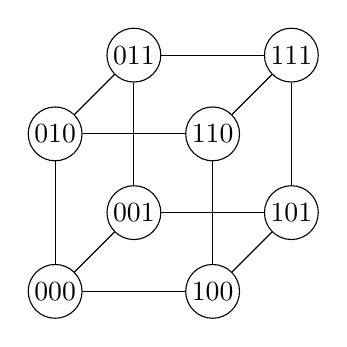
\begin{tikzpicture}[scale=2, every node/.style={circle, draw, fill=white, inner sep=1.2pt}]
% front square
\node (000) at (0,0) {$000$};
\node (100) at (1,0) {$100$};
\node (110) at (1,1) {$110$};
\node (010) at (0,1) {$010$};

% back square
\node (001) at (0.5,0.5) {$001$};
\node (101) at (1.5,0.5) {$101$};
\node (111) at (1.5,1.5) {$111$};
\node (011) at (0.5,1.5) {$011$};

% edges of front square
\draw (000)--(100)--(110)--(010)--(000);

% edges of back square
\draw (001)--(101)--(111)--(011)--(001);

% edges between front and back
\draw (000)--(001);
\draw (100)--(101);
\draw (110)--(111);
\draw (010)--(011);
\end{tikzpicture}
\end{center}
\end{example}

\bigskip

The symmetries of \(Q_n\) form the \emph{hyperoctahedral group}: these are all the transformations you get by:
\begin{itemize}
\item translating every vertex by the same binary vector (bitwise XOR),
\item permuting the coordinate positions.
\end{itemize}

We now state and prove the precise structure.

\begin{theorem}
For every \(n \ge 1\),
\[
\mathrm{Aut}(Q_n) \cong H \rtimes S_n,
\]
where \(H \cong (\mathbb{Z}_2)^n\) is the group of translations \(x \mapsto x \oplus t\) (bitwise addition mod 2), and \(S_n\) acts by permuting coordinates.  

Equivalently, \(\mathrm{Aut}(Q_n)\) is the wreath product \(\mathbb{Z}_2 \wr S_n\) (the hyperoctahedral group). In particular,
\[
|\mathrm{Aut}(Q_n)| = 2^n \, n!.
\]
\end{theorem}

\begin{proof}
\textbf{Step 1: Building the obvious automorphisms.}  

Let  
\[
H = \{ \tau_t : t \in \{0,1\}^n \}
\]
where \(\tau_t(x) = x \oplus t\) (bitwise addition mod 2). Each \(\tau_t\) preserves Hamming distances, hence is an automorphism. The set \(H\) is a subgroup of \(\mathrm{Aut}(Q_n)\) isomorphic to \((\mathbb{Z}_2)^n\), called the \emph{translation group}.  

For any permutation \(\pi \in S_n\), define
\[
\sigma_\pi(x_1, \dots, x_n) = (x_{\pi^{-1}(1)}, \dots, x_{\pi^{-1}(n)}).
\]
This just permutes coordinates, so \(\sigma_\pi \in \mathrm{Aut}(Q_n)\).  

Translations and coordinate permutations interact via  
\[
\sigma_\pi \tau_t \sigma_\pi^{-1} = \tau_{t^\pi}
\]
(where \(t^\pi\) has its coordinates permuted by \(\pi\)), so together they form a subgroup \(H \rtimes S_n\) of \(\mathrm{Aut}(Q_n)\) of size \(2^n n!\).

\medskip

\textbf{Step 2: Every automorphism is of this form.}  

Let \(g \in \mathrm{Aut}(Q_n)\). First, note that the neighbors of \(0 = (0, \dots, 0)\) are exactly the \(n\) unit vectors \(e_1, \dots, e_n\).  

If \(g(0) = v\), compose with the translation \(\tau_v\) to get \(g' = \tau_v \circ g\) which fixes \(0\). So it suffices to consider automorphisms fixing \(0\).  

Any \(h \in \mathrm{Aut}(Q_n)\) fixing \(0\) must permute the set \(\{e_1, \dots, e_n\}\). This gives some \(\pi \in S_n\) with \(h(e_i) = e_{\pi(i)}\) for all \(i\). Then \(\sigma_{\pi^{-1}} \circ h\) fixes \(0\) and all \(e_i\).  

But every vertex of \(Q_n\) is the XOR of certain \(e_i\)'s. Since an automorphism preserves adjacency, fixing \(0\) and all \(e_i\) forces it to fix all vertices. Therefore \(h = \sigma_\pi\).  

Thus any \(g\) can be written as \(\tau_t \circ \sigma_\pi\) for some \(t\) and \(\pi\), so \(\mathrm{Aut}(Q_n) \subseteq H \rtimes S_n\).

\medskip

\textbf{Step 3: Conclusion.}  

We have \(H \rtimes S_n \subseteq \mathrm{Aut}(Q_n)\) by construction, and \(\mathrm{Aut}(Q_n) \subseteq H \rtimes S_n\) by the above argument. Therefore
\[
\mathrm{Aut}(Q_n) = H \rtimes S_n \cong (\mathbb{Z}_2)^n \rtimes S_n,
\]
with \(|\mathrm{Aut}(Q_n)| = 2^n n!\).
\end{proof}




\section{Line graphs}

\begin{definition}
The \emph{line graph} of a graph \(X\), denoted \(L(X)\), is the graph whose
vertex set is \(E(X)\), the set of edges of \(X\), with two vertices of
\(L(X)\) adjacent if and only if the corresponding edges of \(X\) are
incident in \(X\).
\end{definition}

\begin{example}
\leavevmode
\begin{itemize}
  \item The star \(K_{1,n}\) has line graph \(K_n\) (all \(n\) edges meet at the center).
  \item The path \(P_n\) has line graph \(P_{n-1}\).
  \item The cycle \(C_n\) is isomorphic to its own line graph.
\end{itemize}
\end{example}

\begin{lemma}
The Petersen graph $P$ is (isomorphic to) the complement of the line graph $L(K_5)$.
\end{lemma}

\begin{proof}
Let $K_5$ be the complete graph on vertex set $[5]=\{1,2,3,4,5\}$.  Denote by $E(K_5)$ the set of its edges.  Recall:
\begin{itemize}
  \item The \emph{line graph} $L(K_5)$ has vertex set $V(L(K_5))=E(K_5)$, and two vertices of $L(K_5)$ are adjacent exactly when the corresponding edges of $K_5$ share a common endpoint.
  \item The \emph{complement} $\overline{L(K_5)}$ has the same vertex set $E(K_5)$, and two vertices are adjacent in $\overline{L(K_5)}$ exactly when the corresponding edges of $K_5$ are \emph{disjoint}.
\end{itemize}

Identify each edge of $K_5$ with the $2$-element subset of $[5]$ that it determines. Then
\[
V(\overline{L(K_5)})=\binom{[5]}{2},
\]
and adjacency in $\overline{L(K_5)}$ is given by
\[
\{i,j\}\sim\{k,\ell\}\quad\Longleftrightarrow\quad \{i,j\}\cap\{k,\ell\}=\varnothing.
\]

But this is exactly the definition of the Kneser graph $K(5,2)$: its vertices are the $2$-subsets of a $5$-set, with two vertices adjacent iff they are disjoint. It is well-known (and elementary to check) that $K(5,2)$ is the Petersen graph $P$. Concretely:
\begin{itemize}
  \item $|\binom{[5]}{2}|=\binom{5}{2}=10$, the Petersen graph has $10$ vertices.
  \item For a given $2$-subset $\{i,j\}$ there are exactly $\binom{3}{2}=3$ disjoint $2$-subsets, so $\overline{L(K_5)}$ is $3$-regular; the Petersen graph is cubic.
  \item The adjacency rule (disjointness of $2$-subsets) matches the standard Petersen construction.
\end{itemize}

Therefore $\overline{L(K_5)}\cong K(5,2)\cong P$, as required.
\end{proof}



\begin{theorem}[Whitney’s theorem]
If \(X\) is a connected graph with \(|V(X)|\geq 5\), then
\[
\mathrm{Aut}(X) \cong \mathrm{Aut}(L(X)).
\]
\end{theorem}

\begin{corollary}
Since \(K_5\) has automorphism group \(S_5\) and \(P\) is the complement of \(L(K_5)\),
it follows that
\[
\mathrm{Aut}(P) \cong S_5.
\]
\end{corollary}

\begin{definition}[Cartesian product of graphs]
Let \(G\) and \(H\) be graphs.  
The \emph{Cartesian product} \(G \square H\) is the graph with vertex set
\[
V(G \square H) = V(G) \times V(H),
\]
and where two vertices \((g,h)\) and \((g',h')\) are adjacent if and only if:
\begin{itemize}
  \item \(g = g'\) and \(hh' \in E(H)\), or
  \item \(h = h'\) and \(gg' \in E(G)\).
\end{itemize}
\end{definition}


\begin{proposition}
The $n$-dimensional hypercube $Q_n$ is the Cartesian product of $n$ copies of $K_2$, i.e.,
\[
Q_n \cong \underbrace{K_2 \square K_2 \square \cdots \square K_2}_{n \text{ times}} = K_2^{\square n}.
\]
\end{proposition}

\begin{proof}
Consider the Cartesian product $K_2 \square K_2 \square \cdots \square K_2$ ($n$ times). Its vertex set consists of all $n$-tuples $(x_1,\dots,x_n)$ with $x_i \in \{0,1\}$. Two vertices $(x_1,\dots,x_n)$ and $(y_1,\dots,y_n)$ are adjacent if and only if they differ in exactly one coordinate.

This adjacency condition is exactly the adjacency rule for $Q_n$, so the graphs are isomorphic:
\[
Q_n \cong K_2^{\square n}.
\]
\end{proof}



\begin{definition}[Disjoint union of graphs]
Given graphs \(X_1, X_2, \dots, X_r\), their \emph{disjoint union} is the graph
\[
X_1 \sqcup X_2 \sqcup \cdots \sqcup X_r
\]
whose vertex set is the disjoint union of the vertex sets \(V(X_1) \sqcup \cdots \sqcup V(X_r)\), and whose edge set is the disjoint union of the edge sets \(E(X_1) \sqcup \cdots \sqcup E(X_r)\).  
In other words, the graphs \(X_i\) appear as disconnected components in the disjoint union.
\end{definition}

\begin{theorem}[Automorphisms of Cartesian products of prime factors]
Let \(X_1, X_2, \dots, X_r\) be connected graphs such that none of the \(X_i\) can be expressed as a Cartesian product of two smaller nontrivial graphs (i.e., each \(X_i\) is \emph{prime} with respect to the Cartesian product).

Then the automorphism group of the Cartesian product
\[
X = X_1 \square X_2 \square \cdots \square X_r
\]
is isomorphic to the automorphism group of the disjoint union
\[
X_1 \sqcup X_2 \sqcup \cdots \sqcup X_r,
\]
that is,
\[
\mathrm{Aut}(X) \cong \mathrm{Aut}(X_1 \sqcup X_2 \sqcup \cdots \sqcup X_r).
\]
\end{theorem}


\begin{corollary}
Let $Q_n$ be the $n$-dimensional hypercube. Then
\[
\mathrm{Aut}(Q_n) \cong \mathbb{Z}_2^n \rtimes \mathrm{Sym}(n),
\]
where $\mathbb{Z}_2^n$ corresponds to flipping coordinates and $\mathrm{Sym}(n)$ to permuting coordinates.
\end{corollary}

\begin{proof}
Since $Q_n \cong nK_2$ and $K_2$ is prime with respect to the Cartesian product, the theorem on automorphisms of Cartesian products implies that
\[
\mathrm{Aut}(Q_n) \cong \mathrm{Aut}(K_2)^n \rtimes \mathrm{Sym}(n) \cong \mathbb{Z}_2^n \rtimes \mathrm{Sym}(n),
\]
as claimed.
\end{proof}



\section{Frucht's Theorem}

\begin{lemma}  
Let $G = \{g_1, \dots, g_n\}$ be a finite group. Construct a colored digraph $D$ with vertices corresponding to the elements of $G$ such that $g_i$ is joined to $g_j$ by a directed edge of color $k$ if $g_i g_j^{-1} = g_k$.  The automorphism group of $D$ is isomorphic to $G$.
\end{lemma}

\begin{proof}  
The right multiplication by any fixed group element $g \in G$, i.e., the mapping 
\[
g_i \mapsto g_i g,
\] 
is an automorphism of $D$. Indeed, if $g_i$ is joined to $g_j$ by an edge of color $k$ (i.e., $g_i g_j^{-1} = g_k$), then
\[
(g_i g)(g_j g)^{-1} = g_i g_j^{-1} = g_k,
\] 
so $g_i g$ is joined to $g_j g$ by an edge of the same color $k$.  

Conversely, let $a$ be any automorphism of $D$ and set $g = a(1)$. We claim that $g_i g = a(g_i)$ for all $i$.  

- Since $(g_i g) g^{-1} = g_i$, $g_i g$ is joined to $g$ by an edge of color $i$, and $g_i$ is the only point with this property.  
- By definition, $g_i$ is joined to $1$ by an edge of color $i$, and since $a$ is an automorphism, $a(g_i)$ is joined to $a(1) = g$ by an edge of color $i$.  
- Hence, $a(g_i) = g_i g$.

It is easy to see that multiplication of elements in $G$ corresponds exactly to composition of the corresponding automorphisms. Therefore,
\[
\mathrm{Aut}(D) \cong G.
\]  
\end{proof}

\medskip

\begin{theorem} (Frucht, 1939)  
For any finite group $G$, there exists a simple graph $X$ such that
\[
\mathrm{Aut}(X) \cong G.
\]
\end{theorem}
\begin{proof}  
Assume $|G| \ge 2$. By the previous lemma, there exists a colored digraph $D$ with $\mathrm{Aut}(D) \cong G$.  

Construct a simple graph $X$ as follows:

1. If $g_i, g_j \in V(D)$ are joined by an edge of color $k$, replace it by a path of length $k+2$, with paths of length 1 attached to each inner vertex, except for the inner vertex next to $g_j$, where we attach a path of length 2 (see Figure below).  
2. Repeat this for every pair $(g_i, g_j)$, then remove all directed edges. Denote the resulting graph by $X$.  

\begin{center}
\includegraphics[width=0.5\textwidth]{Frucht.png}
\end{center}

\noindent\textbf{Claim:} $\mathrm{Aut}(X) \cong \mathrm{Aut}(D) \cong G$.  

Each automorphism of $D$ induces a unique automorphism of $X$.  Conversely, let $a \in \mathrm{Aut}(X)$. The vertices of $D$ are exactly those vertices of $X$ that are neither cutpoints nor endpoints. Hence, $V(D)$ is invariant under $a$. The new paths with attached shorter paths are exactly the components of $X - V(D)$, and $a$ maps them onto each other. A path of length $k$ must map to a path of the same length, and the end with the longer attached path maps correspondingly.  

Thus, if $g_i$ is connected to $g_j$ by an edge of color $k$, then so is $a(g_i)$ to $a(g_j)$. Hence, $a$ yields an automorphism of $D$, and the correspondence is bijective.  

Therefore, 
\[
\mathrm{Aut}(X) \cong \mathrm{Aut}(D) \cong G.
\]  

\end{proof}


\subsection*{Asymmetric Graphs}



\begin{definition}
A graph is called \emph{asymmetric} if it has no nontrivial automorphisms, i.e., the only automorphism is the identity.
\end{definition}


\begin{example}
Consider the graph \(G\) with vertex set \(V = \{1,2,3,4,5,6\}\) and edges
\[
E = \{12, 23, 34, 24, 35, 56\}.
\]

The graph can be drawn as follows:

\begin{center}
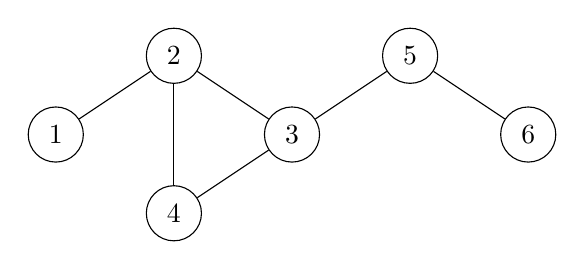
\begin{tikzpicture}[scale=1, every node/.style={circle,draw,minimum size=7mm,inner sep=0pt}]
  \node (1) at (0,0) {1};
  \node (2) at (1.5,1) {2};
  \node (3) at (3,0) {3};
  \node (4) at (1.5,-1) {4};
  \node (5) at (4.5,1) {5};
  \node (6) at (6,0) {6};

  \draw (1) -- (2);
  \draw (2) -- (3);
  \draw (3) -- (4);
  \draw (2) -- (4);
  \draw (3) -- (5);
  \draw (5) -- (6);
\end{tikzpicture}
\end{center}

This graph is \textbf{asymmetric}, meaning it has no nontrivial automorphisms.

\textit{Reason:} Each vertex has a unique adjacency pattern:
\begin{itemize}
  \item Vertex 1 has degree 1 and is only connected to vertex 2.
  \item Vertex 6 has degree 1 and is only connected to vertex 5.
  \item Vertex 2 has degree 3, connected to vertices 1, 3, and 4.
  \item Vertex 4 has degree 2, connected to vertices 2 and 3.
  \item Vertex 3 has degree 3, connected to vertices 2, 4, and 5.
  \item Vertex 5 has degree 2, connected to vertices 3 and 6.
\end{itemize}

No non-identity permutation of vertices preserves the adjacency relations, hence \(\mathrm{Aut}(G) = \{e\}\), the trivial group.This graph is asymmetric; that is, it has only the identity automorphism. Intuitively, each vertex has a unique neighborhood structure preventing any nontrivial vertex permutation that preserves adjacency.
\end{example}

\begin{theorem}
For every integer $n\ge 6$ there exists an asymmetric simple graph on $n$ vertices.
\end{theorem}

\begin{proof}
We split into the base case $n=6$ and a uniform construction for all $n\ge 7$.

\smallskip
\noindent\textbf{Base case $n=6$.} 
Consider the graph $G_6$ with vertex set $\{v_1,\dots,v_6\}$ and edges
\[
v_1v_2,\ v_2v_3,\ v_3v_4,\ v_4v_1 \quad(\text{a $4$-cycle}),\qquad
v_2v_5,\ v_5v_3 \quad(\text{a ``roof''}),\qquad
v_2v_6\quad(\text{a pendant edge}).
\]
(Equivalently: a ``house'' graph on $\{v_1,\dots,v_5\}$ with an extra leaf $v_6$ attached to $v_2$.)

We claim $\mathrm{Aut}(G_6)=1$. Compute the degree sequence:
\[
\deg(v_1)=\deg(v_4)= \deg(v_5)=2,\ \deg(v_2)=4,\ \deg(v_3)=3,\,\ \deg(v_6)=1.
\]



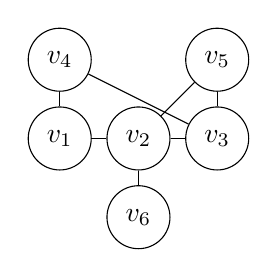
\begin{tikzpicture}[vertex/.style={circle,draw,fill=white,inner sep=1.5pt,minimum size=8mm,font=\sffamily},
                    scale=1]
  % coordinates chosen to resemble the picture in the discussion
  \node[vertex] (v_1) at (0,0)  {$v_1$};
  \node[vertex] (v_2) at (1,0)  {$v_2$};
  \node[vertex] (v_3) at (2,0)  {$v_3$};
  \node[vertex] (v_4) at (0,1)  {$v_4$};
  \node[vertex] (v_5) at (2,1)  {$v_5$};
  \node[vertex] (v_6) at (1,-1) {$v_6$};

  % edges: 4-cycle 1-2-3-4-1
  \draw (v_1) -- (v_2);
  \draw (v_2) -- (v_3);
  \draw (v_3) -- (v_4);
  \draw (v_4) -- (v_1);

  % roof edges 2-5, 5-3
  \draw (v_2) -- (v_5);
  \draw (v_5) -- (v_3);

  % pendant edge 2-6
  \draw (v_2) -- (v_6);

  % optional: label edges (comment out if undesired)
  %\node at (1.0,0.2) {$(1,2)$};
\end{tikzpicture}

\vspace{6pt}

Any automorphism fixes $v_2,v_3,v_6$. Among the degree-$2$ vertices, $v_5$ is uniquely
characterized as the \emph{only} degree-$2$ vertex that lies on a triangle ($v_2v_5v_3$),
so $v_5$ is fixed. The remaining degree-$2$ vertices are $v_1$ and $v_4$, and they are
distinguished by their distances to $v_6$:
\[
d(v_1,v_6)=2 \quad\text{while}\quad d(v_4,v_6)=3.
\]
Hence $v_1$ and $v_4$ are fixed as well. Therefore every vertex is fixed, so $\mathrm{Aut}(G_6)=1$,
and $G_6$ is asymmetric.

\smallskip
\noindent\textbf{All $n\ge 7$.} 
We construct an \emph{asymmetric tree} $T_n$ on $n$ vertices. Let $u$ be a new vertex.
Attach to $u$ three internally-disjoint paths of distinct lengths $1,2,$ and $n-4$,
all meeting at $u$ and otherwise disjoint. (So the total number of vertices is
$1+(1+2+(n-4))=n$, and the three branches have different lengths because $n-4\ge 3$.)

We show $\mathrm{Aut}(T_n)=1$. First, $u$ is the unique vertex of degree $3$, hence is fixed by
every automorphism. Deleting $u$ decomposes $T_n$ into three components which are paths of
lengths $1,2,$ and $n-4$. Since these lengths are pairwise distinct, the components are
pairwise non-isomorphic, so each branch is setwise fixed by any automorphism. On a path,
there is a unique vertex at each distance from the attachment point $u$, hence each branch
is fixed pointwise by any automorphism that fixes $u$. Consequently every vertex of $T_n$
is fixed, and $\mathrm{Aut}(T_n)=1$.

\smallskip
Combining the base case $n=6$ with the tree construction for all $n\ge 7$ proves the claim.
\end{proof}


\textbf{Exercises:}
\begin{enumerate}
  \item Show that any automorphism of a tree fixes either a vertex or an edge; deduce that a finite tree has a nonempty fixed point set for $\mathrm{Aut}$.
  \item Determine $\mathrm{Aut}(K_{m}\square K_n)$ for $m\neq n$ and for $m=n$.
  %\item Prove that $\Aut(K_{n,n}\setminus M)$ (remove a perfect matching $M$) is $(S_n\times S_n)$; when does an extra $\Bbb Z_2$ appear?
  %\item Let $X$ be vertex-transitive and not complete. Prove $\Aut(X)$ acts transitively on $E(X)$ iff $X$ is edge-transitive.
  \item (Frucht’s theorem, challenge) Every finite group is the automorphism group of some $3$-regular graph. State it and read about the Frucht graph as an example.
  
  \item If $q\equiv 1 \pmod 4$ is a prime power, the Paley graph $P(q)$ has vertex set $\Bbb F_q$ with two distinct vertices $x, y \in \mathbb{F}_q$ are adjacent if and only if their difference is a nonzero square in $\mathbb{F}_q$:
\[
\{x, y\} \in E(P(q)) \quad \iff \quad x - y \in (\mathbb{F}_q^\times)^2.
\]. Then show that
\[
\mathrm{Aut}(P(q)) \supseteq \left\{ x \mapsto a x + b \;\middle|\; a \in (\mathbb{F}_q^\times)^2,\, b \in \mathbb{F}_q \right\} \rtimes \mathrm{Gal}(\mathbb{F}_q/\mathbb{F}_p),
\]
(Let $q$ be a prime power with $q \equiv 1 \pmod 4$, and let $P(q)$ be the Paley graph with vertex set $\mathbb{F}_q$, where two vertices $x,y \in \mathbb{F}_q$ are adjacent if and only if
\[
x-y \in (\mathbb{F}_q^\times)^2,
\]
the set of nonzero squares in $\mathbb{F}_q$.



For any $b \in \mathbb{F}_q$, define the translation
\[
\tau_b: x \mapsto x+b.
\]
If $x \sim y$ in $P(q)$, then $x-y \in (\mathbb{F}_q^\times)^2$, so
\[
\tau_b(x) - \tau_b(y) = (x+b)-(y+b) = x-y \in (\mathbb{F}_q^\times)^2.
\]
Thus, $\tau_b$ is an automorphism. The set of all translations forms a group isomorphic to $(\mathbb{F}_q,+)$.



Let $a \in (\mathbb{F}_q^\times)^2$ be a nonzero square, and define
\[
\mu_a: x \mapsto ax.
\]
If $x \sim y$, then $x-y$ is a square, so
\[
\mu_a(x) - \mu_a(y) = a(x-y)
\]
is also a square. Hence, $\mu_a$ is an automorphism. The set of all such $\mu_a$ forms a group of order $(q-1)/2$.



Let $\sigma \in \mathrm{Gal}(\mathbb{F}_q / \mathbb{F}_p)$, where $q = p^n$ and $p$ is the characteristic of $\mathbb{F}_q$. Then $\sigma$ is a field automorphism:
\[
x \mapsto \sigma(x), \quad x \in \mathbb{F}_q.
\]
If $x \sim y$, then $x-y$ is a square, and
\[
\sigma(x) - \sigma(y) = \sigma(x-y)
\]
is still a square because field automorphisms preserve multiplicative structure. Therefore, $\sigma$ is an automorphism of $P(q)$.



Combining the above, any automorphism of the form
\[
x \mapsto a\,\sigma(x) + b, \quad a \in (\mathbb{F}_q^\times)^2, \; b \in \mathbb{F}_q, \; \sigma \in \mathrm{Gal}(\mathbb{F}_q/\mathbb{F}_p),
\]
preserves adjacency. These form the group
\[
\mathrm{Aut}(P(q)) \supseteq \left\{ x \mapsto a x + b \;\middle|\; a \in (\mathbb{F}_q^\times)^2,\, b \in \mathbb{F}_q \right\} \rtimes \mathrm{Gal}(\mathbb{F}_q/\mathbb{F}_p),
\]
where the semidirect product $\rtimes$ encodes that the Galois automorphisms act on both the additive and multiplicative parts.
).

\item Let $H(d,q)$ be the Hamming graph (vertices $\{0,\dots,q-1\}^d$, adjacent if they differ in exactly one coordinate). Then show that
\[
\mathrm{Aut}(H(d,q)) \] has a subgroup isomorphic to \[ S_q \wr S_d \;=\; (S_q)^d \rtimes S_d,
\]
acting by independent symbol permutations in each coordinate and by permuting coordinates.
\end{enumerate}

\section*{Sage code for Paley graph:}
\begin{lstlisting}[language=Python]
# Construct Paley graph
q = 9
P = graphs.PaleyGraph(q)

# Automorphism group
A = P.automorphism_group()
print("Order of Aut(P(9)):", A.order())
print("Generators:")
for g in A.gens():
    print(g)
\end{lstlisting}

\paragraph{Explanation:}  
The automorphism group $\mathrm{Aut}(P(q))$ acts on the vertices $\mathbb{F}_q$. It contains:

\begin{itemize}
  \item Translations: $x \mapsto x + a$, for $a \in \mathbb{F}_q$
  \item Multiplications by nonzero squares: $x \mapsto b x$, $b \in (\mathbb{F}_q^\times)^2$
  \item Field automorphisms: $x \mapsto x^p$ (Frobenius map)
\end{itemize}


\paragraph{Example output (order and generators):}
\begin{verbatim}
Order of Aut(P(9)): 216
Generators:
(0,1,2)(3,4,5)(6,7,8)
(0,3)(1,4)(2,5)(6,7)
...
\end{verbatim}


\section*{ Hamming Graph $H(d,q)$}

\paragraph{Sage code:}
\begin{lstlisting}[language=Python]
# Construct Hamming graph
d = 3
q = 2
H = graphs.HammingGraph(d, q)

# Automorphism group
A = H.automorphism_group()
print("Order of Aut(H(3,2)):", A.order())
print("Generators:")
for g in A.gens():
    print(g)
\end{lstlisting}

\noindent\textbf{Explanation:}  
The automorphism group $\mathrm{Aut}(H(d,q))$ is the wreath product
\[
\mathrm{Aut}(H(d,q)) \cong S_q \wr S_d,
\]
where $S_q$ acts on each coordinate and $S_d$ permutes the coordinates.

\paragraph{Example output (order and generators):}
\begin{verbatim}
Order of Aut(H(3,2)): 48
Generators:
(0,1)
(0,4)(1,5)(2,6)(3,7)
...
\end{verbatim}



\begin{definition}[Graph Homomorphism]
Let $G=(V,E)$ and $H=(V',E')$ be simple graphs.  
A \emph{graph homomorphism} is a map
\[
f:V \to V'
\]
such that whenever $uv \in E$ we have $f(u)f(v) \in E'$.  
That is, adjacency is preserved.

An \emph{endomorphism} of a graph $G$ is a homomorphism $f:G \to G$.  
\end{definition}

We write $\alpha(G)$ for the \emph{independence number} of $G$, the size of a largest independent set in $G$.

\textbf{Exercises:}
\begin{enumerate}
\item Let $P$ denote the Petersen graph, show that $\alpha(P) = 4$, and that every independent set of size $4$ is a \emph{star} of the form
\[
\mathcal{S}_t = \big\{ \{t,x\} : x \in \{1,2,3,4,5\} \setminus \{t\} \big\}
\]
for some $t \in \{1,\dots,5\}$.  



\item Show that every endomorphism of the Petersen graph $P$ is an automorphism.


(Hint:
Identify vertices of $P$ with the $2$-subsets of $\{1,2,3,4,5\}$.  
For each $t \in \{1,\dots,5\}$, let
\[
\mathcal{S}_t = \big\{ \{t,x\} : x \neq t \big\}
\]
be the star at $t$, an independent set of size $4$ by Fact~A.

 
If $I \subseteq V(P)$ is independent then $f(I)$ is independent, because $f$ preserves adjacency.  
Thus $f(\mathcal{S}_t)$ is an independent set of size $\le 4$.

%\textbf{Step 2: Maximum independent sets map to maximum independent sets.}  
Since $\mathcal{S}_t$ is maximum, $|f(\mathcal{S}_t)| = 4$ and hence $f(\mathcal{S}_t)$ is itself a star.  
Therefore there exists a map
\[
\pi : \{1,\dots,5\} \longrightarrow \{1,\dots,5\}, \quad f(\mathcal{S}_t) = \mathcal{S}_{\pi(t)}.
\]

%\textbf{Step 3: $\pi$ is a permutation.}  
For $i \neq j$ we have $\mathcal{S}_i \cap \mathcal{S}_j = \{\{i,j\}\}$.  
Applying $f$ gives
\[
\{f(\{i,j\})\} 
= f(\mathcal{S}_i \cap \mathcal{S}_j) 
= f(\mathcal{S}_i) \cap f(\mathcal{S}_j) 
= \mathcal{S}_{\pi(i)} \cap \mathcal{S}_{\pi(j)}.
\]
If $\pi(i) = \pi(j)$ the right-hand side would have size $4$, a contradiction.  
Thus $\pi$ is injective, hence a permutation of $\{1,\dots,5\}$.

%\textbf{Step 4: $f$ is induced by $\pi$.}  
If $v = \{i,j\}$ then $v = \mathcal{S}_i \cap \mathcal{S}_j$, so
\[
f(\{i,j\}) 
= f(\mathcal{S}_i \cap \mathcal{S}_j) 
= \mathcal{S}_{\pi(i)} \cap \mathcal{S}_{\pi(j)} 
= \{\pi(i),\pi(j)\}.
\]
Hence $f$ is exactly the vertex map induced by the permutation $\pi$.

%\textbf{Step 5: Conclusion.}  
Since $\pi$ is a permutation, $f$ is bijective and its inverse is the homomorphism induced by $\pi^{-1}$.  
Therefore $f$ is an automorphism.)

\textbf{remark:}
This constructive exercises show that  $P$ is a \emph{core}: every endomorphism is an automorphism.


\item Show that the Complete graphs $K_n$ for $n \geq 1$, the Odd cycles $C_{2k+1}$and   the Complete bipartite graphs $K_{m,n}$ with $m \neq n$ and $\min(m,n) \geq 2$ are core. Can you give another example?

\end{enumerate}



\chapter{Groups}

In this chapter, we provide the necessary background in group theory and permutation groups that will be essential for our subsequent discussion of graph automorphisms and isomorphism problems. The theory of group actions, orbits, and stabilizers forms the foundation for understanding how symmetries operate on combinatorial structures such as graphs. We begin with basic definitions and properties of permutation groups, then develop the key results that connect group theory to graph theory, including Burnside's lemma for counting orbits and the fundamental concepts of primitivity and orbitals. These tools will be indispensable when we analyze the automorphism groups of graphs and study graph isomorphism classes in later chapters

\section{Permutation Groups}



The set of all permutations of a set $V$ is denoted by $\mathrm{Sym}(V)$, or simply $\mathrm{Sym}(n)$ when $|V| = n$. A \textbf{permutation group} on $V$ is a subgroup of $\mathrm{Sym}(V)$.

If $X$ is a graph with vertex set $V$, then each automorphism of $X$ is a permutation of $V$, so $\mathrm{Aut}(X)$ is a permutation group.

A \textbf{permutation representation} of a group $G$ is a homomorphism from $G$ into $\mathrm{Sym}(V)$ for some set $V$. This is also referred to as an \textbf{action} of $G$ on $V$, in which case we say that $G$ \textbf{acts on} $V$. A representation is \textbf{faithful} if its kernel is the identity group.



A group $G$ acting on a set $V$ induces several other actions. If $S \subseteq V$ and $g \in G$, the \textbf{translate} $S^g$ is again a subset of $V$. Thus each element of $G$ determines a permutation of the subsets of $V$, giving an action of $G$ on the power set $2^V$.  

More precisely, $|S^g| = |S|$, so for any fixed $k$, the action of $G$ on $V$ induces an action on the $k$-subsets of $V$. Similarly, $G$ acts on the ordered $k$-tuples of elements of $V$.

\bigskip\noindent\textbf{Exercise}
Let $G$ act on $V$. Show that $G$ acts on $2^V$ via $S \mapsto S^g$, and on the set of $k$-element subsets of $V$ for any fixed $k$.




Suppose $G$ is a permutation group on $V$. A subset $S \subseteq V$ is \textbf{$G$-invariant} if $S^g \subseteq S$ for all $g \in G$. If $S$ is invariant under $G$, then each $g \in G$ permutes the elements of $S$. Let $g|_S$ denote the \textbf{restriction of $g$ to $S$}. Then the mapping
\[
g \mapsto g|_S
\]
is a homomorphism from $G$ into $\mathrm{Sym}(S)$, and its image is a permutation group on $S$, denoted $G|_S$.

\bigskip\noindent\textbf{Exercise}
Prove that $g \mapsto g|_S$ is a group homomorphism.


A permutation group $G$ on $V$ is \textbf{transitive} if for any $x, y \in V$, there exists $g \in G$ such that $x^g = y$. A $G$-invariant subset $S \subseteq V$ is an \textbf{orbit} if $G|_S$ is transitive on $S$.  

\bigskip\noindent\textbf{Exercise} Show that for any $x \in V$, the set
\[
x^G := \{ x^g : g \in G \}
\]
is the orbit of $G$ containing $x$.


\begin{lemma}\label{lem:orbit-partition}
The orbits of $G$ on $V$ form a partition of $V$. Moreover, any $G$-invariant subset is a union of orbits.
\end{lemma}

\begin{proof}
For any $x, y \in V$, either $x^G = y^G$ or $x^G \cap y^G = \emptyset$. If $x^G \cap y^G \neq \emptyset$, then there exist $g, h \in G$ such that $x^g = y^h$. Then $y = x^{gh^{-1}}$, so $y \in x^G$ and thus $y^G \subseteq x^G$. Similarly, $x^G \subseteq y^G$, so $x^G = y^G$. The second statement follows from the fact that orbits are minimal $G$-invariant subsets.
\end{proof}

\bigskip\noindent\textbf{Exercise}
Prove that the following are equivalent for a non-empty subset $S \subseteq V$:
\begin{enumerate}
\item $S$ is an orbit of $G$
\item $S$ is a minimal $G$-invariant subset
\item For any $x, y \in S$, there exists $g \in G$ such that $x^g = y$
\item $S = x^G$ for some $x \in S$
\end{enumerate}




Let $G$ be a permutation group on $V$. For $x \in V$, the \textbf{stabilizer} of $x$ is
\[
G_x := \{ g \in G : x^g = x \}.
\]

\begin{lemma}\label{lem:stabilizer-subgroup}
For any $x \in V$, $G_x$ is a subgroup of $G$.
\end{lemma}

\begin{proof}
The identity permutation fixes $x$. If $g,h \in G_x$, then $x^{gh} = (x^g)^h = x^h = x$, so $gh \in G_x$. If $g \in G_x$, then $x^{g^{-1}} = (x^g)^{g^{-1}} = x$, so $g^{-1} \in G_x$.
\end{proof}

For distinct points $x_1, \dots, x_r \in V$, the \textbf{pointwise stabilizer} is
\[
G_{x_1, \dots, x_r} := \bigcap_{i=1}^r G_{x_i}.
\]
For $S \subseteq V$, the \textbf{setwise stabilizer} is
\[
G_S := \{ g \in G : S^g = S \}.
\]
Clearly, $G_{x_1, \dots, x_r} \subseteq G_S$ if $S = \{x_1, \dots, x_r\}$.

\bigskip\noindent\textbf{Exercise}
Let $G$ act on $V$ and let $S \subseteq V$. Prove that:
\begin{enumerate}
\item $G_S$ is a subgroup of $G$
\item If $S$ is finite, then $G_S$ is the largest subgroup of $G$ that leaves $S$ invariant as a set
\item $G_S$ acts on $S$ and the kernel of this action is $G_{(S)} := \bigcap_{x \in S} G_x$
\end{enumerate}




\begin{lemma}\label{lem:coset-mapping}
Let $G$ act on $V$, and let $S$ be an orbit. If $x, y \in S$, the set of elements of $G$ mapping $x$ to $y$ is a \textbf{right coset} of $G_x$. Conversely, all elements in a right coset of $G_x$ map $x$ to the same point in $S$.
\end{lemma}

\begin{proof}
Since $G$ is transitive on $S$, there exists $g \in G$ such that $x^g = y$. If $h \in G$ and $x^h = y$, then $hg^{-1} \in G_x$, hence $h \in G_x g$. Conversely, any $hg \in G_x g$ satisfies $x^{hg} = (x^h)^g = x^g = y$.
\end{proof}

\begin{theorem}[Orbit-Stabilizer Theorem]\label{thm:orbit-stabilizer}
Let $G$ act on $V$ and $x \in V$. Then
\[
|G| = |x^G| \cdot |G_x|.
\]
\end{theorem}

\begin{proof}
By Lemma \ref{lem:coset-mapping}, points of $x^G$ correspond bijectively to the right cosets of $G_x$. Each coset has $|G_x|$ elements, giving $|G| = |x^G| \cdot |G_x|$.
\end{proof}

\bigskip\noindent\textbf{Exercise}
Let $G$ be a finite group acting on a finite set $V$.
\begin{enumerate}
\item Prove that for any $x \in V$, $|x^G|$ divides $|G|$.
\item If $G$ is transitive on $V$, show that $|V|$ divides $|G|$.
\item If $G$ is $2$-transitive on $V$, show that $|V|(|V|-1)$ divides $|G|$.
\end{enumerate}




\begin{theorem}[Frattini Argument]\label{thm:frattini}
Let $G$ be a group acting on a set $X$. Let $H \le G$ be a subgroup which acts transitively on $X$. For any $\alpha \in X$ let $G_\alpha = \{ g \in G : g \cdot \alpha = \alpha \}$ be the stabilizer of $\alpha$. Then
\[
G = H G_\alpha.
\]
Equivalently, every $g \in G$ can be written as $g = hk$ with $h \in H$ and $k \in G_\alpha$.
\end{theorem}

\begin{proof}
Fix $\alpha \in X$ and let $g \in G$. Since $H$ is transitive, there exists $h \in H$ with $\alpha^h = \alpha^g$. Hence $\alpha^{h^{-1}g} = \alpha$, so $h^{-1}g \in G_\alpha$. Therefore $g = h(h^{-1}g) \in H G_\alpha$. Since $g$ was arbitrary, $G \subseteq H G_\alpha$, and the reverse inclusion is trivial.
\end{proof}

\bigskip\noindent\textbf{Exercise}
 If $G$ is finite and $P$ is a Sylow $p$-subgroup and $N$ be a normal subgroup of $G$ containing $P$, show $G = N_G(P) N$ .







\bigskip
For $g,h \in G$, the element $g^{-1}hg$ is \textbf{conjugate} to $h$. The set of all elements conjugate to $h$ is called its \textbf{conjugacy class}. If $H \le G$ and $g \in G$, define
\[
g^{-1} H g := \{ g^{-1} h g : h \in H \}.
\]
This is a subgroup conjugate to $H$.


\begin{lemma}[Conjugation of Stabilizers]\label{lem:conjugate-stabilizer}
Let $G$ act on $V$, and let $x \in V$. If $y = x^g$ for some $g \in G$, then
\[
g^{-1} G_x g = G_y.
\]
\end{lemma}

\begin{proof}
We prove both inclusions:

\textbf{Step 1: Show $g^{-1} G_x g \subseteq G_y$.}  
Let $h \in G_x$, so $x^h = x$. Then
\[
y^{g^{-1} h g} = (x^g)^{g^{-1} h g} = x^{h g} = (x^h)^g = x^g = y,
\]
hence $g^{-1} h g \in G_y$.

\textbf{Step 2: Show $G_y \subseteq g^{-1} G_x g$.}  
Let $k \in G_y$, so $y^k = y$. Then
\[
(x^g)^k = x^g \implies x^{g k g^{-1}} = x \implies g k g^{-1} \in G_x \implies k \in g^{-1} G_x g.
\]

\textbf{Conclusion:} Both inclusions hold, hence $g^{-1} G_x g = G_y$.
\end{proof}

\bigskip\noindent\textbf{Exercise}\label{ex:conjugate-stabilizers}
Let $G$ act on $V$, and let $x, y \in V$ be in the same orbit.
\begin{enumerate}
\item Show that if $G$ is abelian, then $G_x = G_y$.
\item Give an example where $G_x \neq G_y$ even though $x$ and $y$ are in the same orbit.
\end{enumerate}


\begin{proof}
\begin{enumerate}
\item If $G$ is abelian, then for any $g \in G$ with $y = x^g$, we have:
\[
G_y = g^{-1} G_x g = G_x
\]
since conjugation is trivial in abelian groups.
\item Consider $G = S_3$ acting on $\{1,2,3\}$. Then:
\begin{itemize}
\item $G_1 = \{(1), (23)\}$
\item $G_2 = \{(1), (13)\}$
\item $G_3 = \{(1), (12)\}$
\end{itemize}
All points are in the same orbit, but the stabilizers are different.
\end{enumerate}
\end{proof}



\begin{theorem}[Burnside / Cauchy-Frobenius]\label{thm:burnside}
Let $G$ act on a finite set $V$. Then the number of orbits of $G$ on $V$ is
\[
\#\text{orbits} = \frac{1}{|G|} \sum_{g \in G} |\mathrm{Fix}(g)|, \quad \mathrm{Fix}(g) := \{ x \in V : x^g = x\}.
\]
\end{theorem}

\begin{proof}
We count the set $S = \{ (g,x) \in G \times V : x^g = x \}$ in two different ways:

\textbf{First count:} For each $g \in G$, there are $|\mathrm{Fix}(g)|$ elements $x \in V$ such that $x^g = x$. Hence:
\[
|S| = \sum_{g \in G} |\mathrm{Fix}(g)|.
\]

\textbf{Second count:} For each $x \in V$, there are $|G_x|$ elements $g \in G$ such that $x^g = x$. Hence:
\[
|S| = \sum_{x \in V} |G_x|.
\]

Let $O_1, \dots, O_m$ be the orbits of $G$ on $V$. For each orbit $O_i$ and for any $x \in O_i$, by the Orbit-Stabilizer Theorem we have:
\[
|O_i| = \frac{|G|}{|G_x|} \quad \text{so} \quad |G_x| = \frac{|G|}{|O_i|}.
\]
Therefore:
\[
\sum_{x \in V} |G_x| = \sum_{i=1}^m \sum_{x \in O_i} |G_x| = \sum_{i=1}^m |O_i| \cdot \frac{|G|}{|O_i|} = m |G|.
\]

Equating both counts:
\[
\sum_{g \in G} |\mathrm{Fix}(g)| = m |G| \implies m = \frac{1}{|G|} \sum_{g \in G} |\mathrm{Fix}(g)|.
\]
\end{proof}

\bigskip\noindent\textbf{Exercise}\label{ex:burnside-applications}
\begin{enumerate}
\item Use Burnside's Lemma to count distinct colorings of the vertices of a square with $n$ colors, modulo rotations/reflections.
%\item Show that if every non-identity element of $G$ fixes at most one point, then either:
%\begin{enumerate}
%\item $G$ is trivial and $|V|=1$, or
%\item $G$ is cyclic of prime order and $|V| = |G|$, or
%\item $G$ is a non-abelian simple group with $|V| \ge |G|$.
%\end{enumerate}
\item Let $G$ act transitively on $V$ with $|V|>1$. Show there exists $g \in G$ with no fixed points.
\end{enumerate}


\begin{proof}
\begin{enumerate}
\item The symmetry group of the square (dihedral group $D_4$) has 8 elements:
\begin{itemize}
\item Identity: fixes all $n^4$ colorings
\item 3 rotations by $90^{\circ}, 270^{\circ}$: fix $n$ colorings (all vertices same color)
\item 1 rotation by $180^\circ$: fixes $n^2$ colorings (opposite vertices same color)
\item 2 reflections through vertices: fix $n^3$ colorings (fixed vertex and its opposite)
\item 2 reflections through edges: fix $n^2$ colorings (pairs of opposite vertices)
\end{itemize}
By Burnside's Lemma: $\frac{1}{8}(n^4 + 2n^3 + 3n^2 + 2n)$.
%\item This is a classical result in permutation group theory. The key observation is that if $g,h \in G$ both fix points, then $[g,h]$ fixes more than one point, leading to a contradiction unless $G$ is abelian.
\item By Burnside's Lemma: $\frac{1}{|G|}\sum_{g \in G} |\mathrm{Fix}(g)| = 1$. Since the identity fixes $|V| > 1$ points, some $g \in G$ must fix fewer than 1 point, i.e., 0 points.
\end{enumerate}
\end{proof}

\section{Orbits on Pairs}



\begin{definition}[Orbitals]
Let $G$ act transitively on $V$. Then $G$ acts naturally on $V \times V$ by $(x,y)^g = (x^g, y^g)$. The orbits of this action are called \textbf{orbitals}. The diagonal $\{(x,x): x \in V\}$ is always an orbital, called the \textbf{diagonal orbital}.
\end{definition}

\begin{definition}[Transpose of an Orbital]
If $n \subseteq V \times V$ is an orbital, its \textbf{transpose} is:
\[
n^T = \{(y,x) : (x,y) \in n\}.
\]
An orbital is \textbf{symmetric} if $n = n^T$.
\end{definition}

\begin{lemma}[Orbital-Stabilizer Correspondence]\label{lem:orbital-correspondence}
Let $x \in V$. There is a one-to-one correspondence between the orbits of $G$ on $V \times V$ and the orbits of $G_x$ on $V$.
\end{lemma}

\begin{proof}
Let $n$ be an orbital, and define $Y_0 = \{y \in V : (x,y) \in n\}$.  

\textbf{Step 1: Show $Y_0$ is an orbit of $G_x$.}  
If $y, y' \in Y_0$, then $(x,y), (x,y') \in n$, so there exists $g \in G$ with $(x,y)^g = (x,y')$. This implies $x^g = x$ and $y^g = y'$, so $g \in G_x$ and $y,y'$ are in the same orbit of $G_x$.

\textbf{Step 2: Conversely.}  
If $y' = y^g$ for $g \in G_x$, then $(x,y)^g = (x,y') \in n$, so $y' \in Y_0$.

\textbf{Step 3: Partition.}  
All $Y_0$ obtained in this way partition $V$, giving a one-to-one correspondence.
\end{proof}

\begin{definition}[Rank of a Permutation Group]
The number of orbits of $G_x$ on $V$ is called the \textbf{rank} of $G$.
\end{definition}

\begin{lemma}[Symmetric Orbital]\label{lem:symmetric-orbital}
Let $n$ be an orbital and $(x,y) \in n$. Then $n = n^T$ (symmetric) if and only if there exists $g \in G$ with $x^g = y$ and $y^g = x$.
\end{lemma}

\begin{proof}
\textbf{($\Rightarrow$)} If $n = n^T$, then $(y,x) \in n$. By definition of orbitals, there exists $g \in G$ with $(x,y)^g = (y,x)$, which implies $x^g = y$ and $y^g = x$.

\textbf{($\Leftarrow$)} If such $g$ exists, then $(x,y)^g = (y,x) \in n$, hence $n \cap n^T \neq \emptyset$. Since orbitals are either disjoint or identical with their transpose, we must have $n = n^T$.
\end{proof}

\begin{definition}[Generously Transitive]
A permutation group $G$ on $V$ is \textbf{generously transitive} if for any two distinct elements $x, y \in V$, there exists $g \in G$ swapping $x$ and $y$.
\end{definition}

\bigskip\noindent\textbf{Exercise}\label{ex:orbital-properties}
\begin{enumerate}
\item Show that $G$ is generously transitive if and only if all orbitals are symmetric.
\item Prove that if $G$ is 2-transitive, then it has rank 2.
\item Give an example of a transitive group that is not generously transitive.
\end{enumerate}


\section{Primitivity}



\begin{definition}[Block of Imprimitivity]
Let $G$ act transitively on $V$. A nonempty subset $B \subseteq V$ is a \textbf{block} if for all $g \in G$, either $B^g = B$ or $B^g \cap B = \emptyset$.
\end{definition}

\begin{definition}[System of Imprimitivity]
The set of distinct translates of a block $B$ forms a \textbf{system of imprimitivity}.
\end{definition}

\begin{definition}[Primitive Group]
A transitive group is \textbf{primitive} if it has no nontrivial blocks (blocks other than singletons and $V$ itself). Otherwise it is \textbf{imprimitive}.
\end{definition}

\begin{lemma}[Primitivity via Maximal Stabilizers]\label{lem:primitivity-maximal}
Let $G$ be transitive on $V$, and $x \in V$. Then $G$ is primitive if and only if $G_x$ is a maximal subgroup of $G$.
\end{lemma}

\begin{proof}
\textbf{($\Rightarrow$)} Suppose $G$ is primitive but $G_x$ is not maximal. Then there exists $H$ with $G_x \subset H \subset G$. Let $B = x^H = \{x^h : h \in H\}$. We show $B$ is a nontrivial block:

For any $g \in G$, either $B^g = B$ or $B^g \cap B = \emptyset$. If $B^g \cap B \neq \emptyset$, then there exist $h_1, h_2 \in H$ such that $x^{h_1 g} = x^{h_2}$, so $h_1 g h_2^{-1} \in G_x \subset H$, hence $g \in H$ and $B^g = B$.

Since $G_x \subset H \subset G$, we have $\{x\} \subset B \subset V$, contradicting primitivity.

\textbf{($\Leftarrow$)} Suppose $G_x$ is maximal but $G$ is imprimitive. Let $B$ be a nontrivial block containing $x$. Then $G_B = \{g \in G : B^g = B\}$ is a subgroup containing $G_x$. Since $B$ is nontrivial, $G_x \subset G_B \subset G$, contradicting maximality of $G_x$.
\end{proof}



\begin{definition}[2-Transitive Group]
A permutation group $G$ on $V$ is \textbf{2-transitive} if it acts transitively on the set of ordered pairs of distinct elements of $V$.
\end{definition}

\begin{lemma}
If $G$ is 2-transitive on $V$, then:
\begin{enumerate}
\item $G$ is primitive
\item $G$ has rank 2 (only the diagonal and non-diagonal orbitals)
\item For any $x \in V$, $G_x$ is transitive on $V \setminus \{x\}$
\end{enumerate}
\end{lemma}

\begin{proof}
\begin{enumerate}
\item If $G$ were imprimitive with block $B$ containing $x$, then for any $y \in B \setminus \{x\}$ and $z \notin B$, there is no $g \in G$ with $(x,y)^g = (x,z)$, contradicting 2-transitivity.
\item The orbitals are exactly $\{(x,x) : x \in V\}$ and $\{(x,y) : x \neq y\}$.
\item Immediate from the definition of 2-transitivity.
\end{enumerate}
\end{proof}



\begin{definition}[Strongly and Weakly Connected Digraph]
Let $D$ be a directed graph.
\begin{itemize}
\item A \textbf{path} is a sequence of vertices $u_0, u_1, \dots, u_r$ with $(u_{i-1}, u_i)$ an arc for each $i$
\item A \textbf{weak path} allows either $(u_{i-1}, u_i)$ or $(u_i, u_{i-1})$ as an arc
\item $D$ is \textbf{strongly connected} if any two vertices can be joined by a path
\item $D$ is \textbf{weakly connected} if any two vertices can be joined by a weak path
\end{itemize}
\end{definition}

\begin{lemma}[Strong/Weak Equivalence]\label{lemma:strong-weak-connected}
Let $D$ be a digraph where every vertex has equal in-valency and out-valency. Then $D$ is strongly connected if and only if it is weakly connected.
\end{lemma}

\begin{proof}
($\Rightarrow$) Trivial, since strong connectivity implies weak connectivity.

($\Leftarrow$) Suppose $D$ is weakly but not strongly connected. Let $D_1, \dots, D_r$ be its strong components. Consider the condensation digraph $D'$ whose vertices are the strong components, with an arc from $D_i$ to $D_j$ if there is an arc from some vertex in $D_i$ to some vertex in $D_j$.

Since $D'$ is acyclic, there exists a strong component $D_i$ with no incoming arcs from other components. But then:
\[
\sum_{v \in D_i} \text{in-valency}(v) = \text{number of arcs within } D_i < \sum_{v \in D_i} \text{out-valency}(v)
\]
since weak connectivity requires at least one outgoing arc from $D_i$ to another component. This contradicts the assumption that in-valency equals out-valency for each vertex.
\end{proof}

\begin{theorem}[Primitivity and Connectivity]\label{thm:primitivity-connectivity}
Let $G$ be transitive on $V$. Then $G$ is primitive if and only if every nondiagonal orbital of $G$ on $V \times V$ is connected as a directed graph.
\end{theorem}

\begin{proof}
\textbf{($\Rightarrow$)} Suppose $G$ is primitive. Let $n$ be a nondiagonal orbital and $(x,y) \in n$. Consider the connected component $C$ of $n$ containing $x$. We show $C = V$.

For any $g \in G$, either $C^g = C$ or $C^g \cap C = \emptyset$. But since $G$ is transitive and $C$ is nonempty, the translates of $C$ cover $V$. If $C^g \cap C \neq \emptyset$ for some $g$, then $C^g = C$. Thus $C$ is a block. Since $G$ is primitive and $C$ contains at least $x$ and $y \neq x$, we must have $C = V$.

\textbf{($\Leftarrow$)} Suppose all nondiagonal orbitals are connected but $G$ is imprimitive. Let $B$ be a nontrivial block containing $x$. Pick $y \in B \setminus \{x\}$ and $z \notin B$. Let $n$ be the orbital containing $(x,y)$.

Since $n$ is connected, there is a path from $x$ to $z$ in $n$. But this path must leave $B$ at some point, contradicting that $B$ is a block (since for any $g \in G$, either $B^g = B$ or $B^g \cap B = \emptyset$).
\end{proof}

\bigskip\noindent\textbf{Exercise}\label{ex:primitivity-exercises}
\begin{enumerate}
\item Show that every 2-transitive group is primitive.
%\item Prove that a primitive group with an abelian normal subgroup is necessarily of prime degree.
\item Give an example of a primitive group that is not 2-transitive.
\item Show that if $G$ is primitive and $N$ is a non-trivial normal subgroup of $G$, then $N$ is transitive.
\end{enumerate}


\begin{proof}
\begin{enumerate}
\item If $G$ is 2-transitive, then for any $x \in V$, $G_x$ is transitive on $V \setminus \{x\}$. If $G$ were imprimitive with block $B$ containing $x$, then $B \setminus \{x\}$ would be a proper $G_x$-invariant subset of $V \setminus \{x\}$, contradicting transitivity.
%\item Let $N$ be an abelian normal subgroup of a primitive group $G$. For any $x \in V$, $N_x$ is normal in $G_x$. The orbits of $N$ form a system of imprimitivity, so by primitivity, $N$ must be transitive. Then $|V| = |N|/|N_x|$. Since $N$ is abelian, all stabilizers $N_x$ are equal, so $|V|$ divides $|N|$. But $N$ is a minimal normal subgroup, so $|V|$ must be prime.
%\item The alternating group $A_4$ acting on 4 points is primitive but not 2-transitive.
\item If $N$ is a normal subgroup of a primitive group $G$, then the orbits of $N$ form a system of imprimitivity. By primitivity, these must be trivial, so $N$ is either trivial or transitive.
\end{enumerate}
\end{proof}


\chapter{Transitive Graphs}

We are going to study the properties of graphs whose automorphism group 
acts vertex transitively. A vertex-transitive graph is necessarily regular. 
One challenge is to find properties of vertex-transitive graphs that are not 
shared by all regular graphs. We will see that transitive graphs are more 
strongly connected than regular graphs in general. Cayley graphs form an 
important class of vertex-transitive graphs; we introduce them and offer 
some reasons why they are important and interesting.

\section{Vertex-Transitive Graphs}

A graph $X$ is vertex transitive (or just transitive) if its automorphism group 
acts transitively on $V(X)$. Thus for any two distinct vertices of $X$ there is 
an automorphism mapping one to the other.

An interesting family of vertex-transitive graphs is provided by the $k$-cubes $Q_k$. 
The vertex set of $Q_k$ is the set of all $2^k$ binary $k$-tuples, with two being adjacent if they differ in precisely one coordinate position. 
We have already met the 3-cube $Q_3$, which is normally just called the cube 


\begin{lemma}
The $k$-cube $Q_k$ is vertex transitive.
\end{lemma}

\begin{proof}
If $v$ is a fixed $k$-tuple, then the mapping
\[
P_v : x \mapsto x + v
\]
(where addition is binary) is a permutation of the vertices of $Q_k$. This mapping is an automorphism because the $k$-tuples $x$ and $y$ differ in precisely one coordinate position if and only if $x + v$ and $y + v$ differ in precisely one coordinate position. There are $2^k$ such permutations, and they form a subgroup $H$ of the automorphism group of $Q_k$. This subgroup acts transitively on $V(Q_k)$ because for any two vertices $x$ and $y$, the automorphism $P_{y-x}$ maps $x$ to $y$.
\end{proof}

Another family of vertex-transitive graphs that we have met before are the circulants. Any vertex can be mapped to any other vertex by using a suitable power of the cyclic permutation described in chapter 1.

The circulants and the $k$-cubes are both examples of a more general construction that produces many, but not all, vertex-transitive graphs. Let $G$ be a group and let $C$ be a subset of $G$ that is closed under taking inverses and does not contain the identity. Then the \emph{Cayley graph} $X(G, C)$ is the graph with vertex set $G$ and edge set
\[
E(X(G, C)) = \{gh : hg^{-1} \in C\}.
\]

If $C$ is an arbitrary subset of $G$, then we can define a directed graph $X(G, C)$ with vertex set $G$ and arc set $\{(g, h) : hg^{-1} \in C\}$. If $C$ is inverse-closed and does not contain the identity, then this graph is undirected and has no loops, and the definition reduces to that of a Cayley graph. 

\begin{theorem}
The Cayley graph $X(G, C)$ is vertex transitive.
\end{theorem}

\begin{proof}
For each $g \in G$ the mapping
\[
P_g : x \mapsto xg
\]
is a permutation of the elements of $G$. This is an automorphism of $X(G, C)$ because
\[
(xg)(yg)^{-1} = x y^{-1},
\]
and so $x \sim y$ if and only if $xg \sim yg$. The permutations $P_g$ form a subgroup of the automorphism group of $X(G, C)$ isomorphic to $G$. This subgroup acts transitively on the vertices of $X(G, C)$ because for any two vertices $g$ and $h$, the automorphism $P_{g^{-1}h}$ maps $g$ to $h$.
\end{proof}

The $k$-cube is a Cayley graph for the elementary abelian group $(\mathbb{Z}_2)^k$, and a circulant on $n$ vertices is a Cayley graph for the cyclic group of order $n$.

Most small vertex-transitive graphs are Cayley graphs, but there are also many families of vertex-transitive graphs that are not Cayley graphs. In particular, the graphs $J(v, k, i)$ are vertex transitive because $\text{Sym}(v)$ contains permutations that map any $k$-set to any other $k$-set, but in general they are not Cayley graphs. We content ourselves with a single example.

\begin{lemma}
The Petersen graph is not a Cayley graph.
\end{lemma}

\begin{proof}
There are only two groups of order 10, the cyclic group $\mathbb{Z}_{10}$ and the dihedral group $D_{10}$. You may verify that none of the cubic Cayley graphs on these groups are isomorphic to the Petersen graph (Exercise: each cayley graph on 10 vertices has girth 4).
\end{proof}



\section{Edge-Transitive Graphs}

A graph $X$ is edge transitive if its automorphism group acts transitively on $E(X)$. It is straightforward to see that the graphs $J(v, k, i)$ are edge transitive, but the circulants are not usually edge transitive.

An \emph{arc} in $X$ is an ordered pair of adjacent vertices, and $X$ is arc transitive if $\text{Aut}(X)$ acts transitively on its arcs. It is frequently useful to view an edge in a graph as a pair of oppositely directed arcs. An arc-transitive graph is necessarily vertex and edge transitive. In this section we will consider the relations between these various forms of transitivity.

The complete bipartite graphs $K_{m,n}$ are edge transitive, but not vertex transitive unless $m = n$, because no automorphism can map a vertex of valency $m$ to a vertex of valency $n$. The next lemma shows that all graphs that are edge transitive but not vertex transitive are bipartite.

\begin{lemma}
Let $X$ be an edge-transitive graph with no isolated vertices. If $X$ is not vertex transitive, then $\text{Aut}(X)$ has exactly two orbits, and these two orbits are a bipartition of $X$.
\end{lemma}

\begin{proof}
Suppose $X$ is edge but not vertex transitive. Suppose that $\{x, y\} \in E(X)$. If $w \in V(X)$, then $w$ lies on an edge and there is an element of $\text{Aut}(X)$ that maps this edge onto $\{x,y\}$. Hence any vertex of $X$ lies in either the orbit of $x$ under $\text{Aut}(X)$, or the orbit of $y$. This shows that $\text{Aut}(X)$ has exactly two orbits. An edge that joins two vertices in one orbit cannot be mapped by an automorphism to an edge that contains a vertex from the other orbit. Since $X$ is edge transitive and every vertex lies in an edge, it follows that there is no edge joining two vertices in the same orbit. Hence $X$ is bipartite and the orbits are a bipartition for it.
\end{proof}



An arc-transitive graph is, as we noted, always vertex and edge transitive. The converse is in general false; we do at least have the next result.

\begin{lemma}
If the graph $X$ is vertex- and edge-transitive, but not arc-transitive, then its valency is even.
\end{lemma}

\begin{proof}
Let $G = \mathrm{Aut}(X)$, and pick a vertex $x \in V(X)$ and a neighbor $y$ of $x$. Let
\[
n = G \cdot (x, y)
\]
be the orbit of the arc $(x, y)$ under $G$.  

Since $X$ is edge-transitive, every edge can be mapped by an automorphism to either $(x, y)$ or $(y, x)$.  
But $X$ is not arc-transitive, so $(y, x) \notin n$. Let
\[
n^T = \{ (v, u) \mid (u, v) \in n \}
\]
be the reversed orbit. Then $n$ and $n^T$ are disjoint, and the edge set of $X$ is
\[
E(X) = n \cup n^T.
\]

Now consider the vertex $x$. Let
\[
d = |\{ z \mid (x, z) \in n \}|
\]
be the out-degree of $x$ in $n$.  

Observe that $(x, y) \in n$ implies $(y, x) \in n^T$. By vertex-transitivity, the out-degree of $x$ in $n$ equals the out-degree of $y$ in $n^T$. But the out-degree of $y$ in $n^T$ counts arcs of the form $(y, z) \in n^T$, which correspond exactly to arcs $(z, y) \in n$. Therefore,
\[
\text{out-degree of } x \text{ in } n = \text{out-degree of } y \text{ in } n^T = \text{in-degree of } x \text{ in } n.
\]

Hence, at vertex $x$, the number of edges from $n$ equals the number from $n^T$, giving total valency
\[
\deg(x) = |\{ z \mid (x,z) \in n \}| + |\{ z \mid (x,z) \in n^T \}| = d + d = 2d.
\]

Since $2d$ is even, the valency of $X$ is even.
\end{proof}


A simple corollary to this result is that a vertex- and edge-transitive graph of odd valency must be arc transitive. 

\section{Semisymmetric graphs and small orders}

\begin{definition}
A graph $X$ is called \emph{semisymmetric} if $X$ is regular and edge-transitive but \emph{not} vertex-transitive.

\end{definition}

The first structural fact is standard and easy to prove.

\begin{proposition}\label{prop:bipartite}
If $X$ is a connected semisymmetric graph then $X$ is bipartite and the automorphism group of $X$ has exactly two vertex-orbits (the two bipartition classes), which are of equal size. In particular the order $|V(X)|$ is even.
\end{proposition}

\begin{proof}
Let $A=\operatorname{Aut}(X)$. Since $X$ is edge-transitive but not vertex-transitive, $A$ acts transitively on the edge-set $E(X)$ but has at least two orbits on $V(X)$. Because every edge has its two endpoints in (possibly different) vertex-orbits, edge-transitivity implies all edges join vertices in different vertex-orbits; otherwise an edge whose endpoints lie in the same orbit could be sent to an edge whose endpoints lie in different orbits, contradicting that vertex-orbits are preserved by automorphisms. Hence every edge joins two distinct vertex-orbits; thus there are no edges inside a vertex-orbit, so each vertex-orbit is an independent set. Therefore $X$ is bipartite, with the bipartition given by the vertex-orbits of $A$.

Let the two orbits have sizes $r$ and $s$. Edge-transitivity and regularity of $X$ imply every vertex has the same degree $k\ge1$. Counting edges from the two sides gives $rk=|E(X)|=sk$, hence $r=s$. Thus the two parts have equal size and $|V(X)|=2r$ is even.
\end{proof}

From Proposition~\ref{prop:bipartite} we immediately get:

\begin{corollary}\label{cor:prime}
There is no semisymmetric graph of prime order $p$ (with $p$ odd).
\end{corollary}

\begin{proof}
By Proposition~\ref{prop:bipartite} the order of any semisymmetric graph is even. A prime $p>2$ is odd, hence impossible. The only prime that is even is $2$, but a graph on two vertices is either a single edge (which is vertex-transitive) or two isolated vertices (not edge-transitive), so there is no semisymmetric graph of order $2$ either.
\end{proof}

Next we rule out order $6$.

\begin{proposition}\label{prop:6}
There is no semisymmetric graph of order $6$.
\end{proposition}

\begin{proof}
By Proposition~\ref{prop:bipartite} a semisymmetric graph on $6$ vertices would be bipartite with two parts of size $3$ and regular of some degree $k$ with $1\le k\le3$.

Consider the possibilities:

\begin{itemize}
\item $k=1$. Then the graph is a perfect matching (three disjoint edges). Such a graph is vertex-transitive (any vertex in the matching is equivalent to any other by a suitable permutation that preserves the matching), so it is not semisymmetric.

\item $k=2$. A connected 2-regular graph on 6 vertices is a $6$-cycle $C_6$, which is vertex-transitive. (If disconnected, it is union of cycles, again vertex-transitive on each component.) Thus not semisymmetric.

\item $k=3$. The unique connected bipartite 3-regular graph with parts of size $3$ is the complete bipartite graph $K_{3,3}$. But $K_{3,3}$ is vertex-transitive: any vertex lies in a part of size $3$ and there is an automorphism sending any vertex to any other (parts can be permuted), so $K_{3,3}$ is vertex-transitive.
\end{itemize}

Hence no case yields a connected regular edge-transitive but not vertex-transitive graph on 6 vertices.
\end{proof}

\begin{example}
 There is no semisymmetric graph of order $3p$.
\end{example}

\begin{proof}
 Let $X$ be a semisymmetric graph of order $3p$. If $|V(X)|=3p$ with $p$ odd, then by Proposition~\ref{prop:bipartite} the order must be even. But $3p$ is odd for odd $p$, so no semisymmetric graph can exist. (The only remaining case is $p=2$, giving $|V|=6$, which was treated in Proposition~\ref{prop:6}.)
\end{proof}


\noindent\textbf{Remark:}

The arguments above use only elementary counting and basic permutation group facts (orbit sizes divide the set size). For orders with small prime factors these constraints are often strong enough to rule out semisymmetric graphs. For larger composite orders semisymmetric graphs do exist (indeed the smallest \emph{nontrivial} semisymmetric graph is the Folkman graph of order $20$, and there are many further constructions), so the impossibility phenomena are primarily a small-order effect.
\bigskip

\noindent\textbf{Example}
The \emph{Folkman graph} is a 4-regular bipartite graph on $20$ vertices. It can be constructed in several equivalent ways:  

\noindent Start with the complete graph $K_{5}$. Subdivide each edge into a path of length two, and then duplicate each of the original five vertices. The resulting bipartite graph has $20$ vertices, each of degree $4$.
 % \item Equivalently, let $V=\mathbb{Z}_{5}\times\{0,1\}$. Vertices $(i,0)$ and $(j,1)$ are adjacent if and only if $i-j\equiv \pm1 \pmod{5}$ or $i-j\equiv \pm2 \pmod{5}$.
\

The Folkman graph is \emph{edge-transitive} but not vertex-transitive. Since it is regular,  it is  an example of a \emph{semisymmetrci graph}.

\begin{figure}[h!]
\centering
\includegraphics[width=0.6\textwidth]{FolkmanGraph.png}
\caption{The Folkman graph, the smallest semi-symmetric graph.}
\label{fig:TutteCoxeter}
\end{figure}
\bigskip
\noindent\textbf{Explanation:}  The green vertices subdivide each edge of 
$K_5$, and the red pairs of vertices are the result of doubling the five vertices of 
$ K_{5}$.
\bigskip

Suppose that $\Gamma$ is a connected $k$-graph and $G$ is a subgroup of the automorphism group $\operatorname{Aut}(\Gamma)$ of $\Gamma$. Then $\Gamma$ is \emph{$G$-semisymmetric} if $G$ acts edge transitively but not vertex transitively on $\Gamma$. Now suppose that $\Gamma$ is a $G$-semisymmetric  graph. Let $\{u, v\}$ be an edge in $\Gamma$. Set $G_u = \operatorname{Stab}_G(u)$, $G_v = \operatorname{Stab}_G(v)$ and $G_{uv} = G_u \cap G_v$.

\bigskip

\noindent\textbf{Exercises:}
Show that
\begin{enumerate}
\item As $G$ acts edge transitively on $\Gamma$ and $u$ is not in the same $G$-orbit as $v$, we have $[G_u : G_{uv}] = [G_v : G_{uv}]=k$. 

\item Suppose that $K \lhd G$ and $K \leq G_{uv}=G_u\cap G_v$. Then $K$ fixes every edge of $\Gamma$ and hence $K = 1$.

\item  As $\Gamma$ is connected, the subgroup $\langle G_u, G_v \rangle$ acts transitively on the edges of $\Gamma$, show that  $G = \langle G_u, G_v \rangle$. 
\end{enumerate}

\bigskip

We have shown that $G$ satisfies:
\begin{itemize}
    \item $G = \langle G_u, G_v \rangle$;
    \item $[G_u : G_u \cap G_v] = [G_v : G_u \cap G_v] = k$; and
    \item no non-trivial subgroup of $G_{uv}$ is normal in $G$.
\end{itemize}

This group theoretic configuration has been studied by Goldschmidt ( see D. M. Goldschmidt, 
``Automorphisms of trivalent graphs'',
\textit{Annals of Mathematics}, 
112 (1980), 377--406.) where it is shown that when $k=3$, the triple $(G_u, G_v, G_{uv})$ is isomorphic (as an amalgam) to one of fifteen possible such triples (see Table 3.1). Thus if $\Gamma$ is $G$-semisymmetric cubic graph, then the structures of $G_u$, $G_v$ and $G_{uv}$ (and the embeddings of $G_{uv}$ into $G_u$ and $G_v$) are known (up to swapping the roles of $u$ and $v$). We call the possible triples of groups appearing in Table 3.1 \emph{Goldschmidt amalgams}.







\begin{table}[h]
\centering
\caption{Goldschmidt Amalgams}
\label{tab:goldschmidt}
\begin{tabular}{lll}
\toprule
\textbf{Name} & \textbf{$(G_1, G_2)$} & \textbf{Completion} \\
\midrule
$G_1$ & $(\mathbb{Z}_3, \mathbb{Z}_3)$ & $\mathbb{Z}_3 \times \mathbb{Z}_3$ \\
$G_1^1$ & $(\operatorname{Sym}(3), \operatorname{Sym}(3))$ & $3^2.2$ \\
$G_2^1$ & $(\operatorname{Sym}(3), \mathbb{Z}_6)$ & $\operatorname{Sym}(3) \times \mathbb{Z}_3$ \\
$G_3^1$ & $(\operatorname{Sym}(3) \times \mathbb{Z}_2, \operatorname{Sym}(3) \times \mathbb{Z}_2)$ & $\operatorname{PSL}_2(11)$ \\
$G_2$ & $(\operatorname{Alt}(4), \operatorname{Sym}(3) \times \mathbb{Z}_2)$ & $\operatorname{PSL}_2(11)$ \\
$G_1^2$ & $(\operatorname{Sym}(4), \operatorname{Dih}(24))$ & $\operatorname{PSL}_2(23)$ \\
$G_2^2$ & $(\operatorname{Sym}(4), (2^2 \times 3).2)$ & $\operatorname{Alt}(7)$ \\
$G_3^2$ & $(\operatorname{Alt}(4) \times \mathbb{Z}_2, \operatorname{Sym}(3) \times \mathbb{Z}_2 \times \mathbb{Z}_2)$ & $\operatorname{Sym}(3) \wr \mathbb{Z}_3$ \\
$G_4^2$ & $(\operatorname{Sym}(4) \times \mathbb{Z}_2, \operatorname{Sym}(3) \times \operatorname{Dih}(8))$ & $\operatorname{Sym}(7)$ \\
$G_3$ & $(\operatorname{Sym}(4), \operatorname{Sym}(4))$ & $\operatorname{Alt}(6), \operatorname{SL}_3(2)$ \\
$G_1^3$ & $(\operatorname{Sym}(4) \times \mathbb{Z}_2, \operatorname{Sym}(4) \times \mathbb{Z}_2)$ & $\operatorname{Sym}(6)$ \\
$G_4$ & $((\mathbb{Z}_4 \times \mathbb{Z}_4).\operatorname{Sym}(3), (Q_8 \circ \mathbb{Z}_4).\operatorname{Sym}(3))$ & $G_2(2)' \cong U_3(3)$ \\
$G_1^4$ & $((\mathbb{Z}_4 \times \mathbb{Z}_4).(\operatorname{Sym}(3) \times \mathbb{Z}_2), (Q_8 \circ Q_8).\operatorname{Sym}(3))$ & $G_2(2)$ ($\eta(G_2, O_2(G_2)) = 1$) \\
$G_5$ & $((\mathbb{Z}_4 \times \mathbb{Z}_4).(\operatorname{Sym}(3) \times \mathbb{Z}_2), (Q_8 \circ Q_8).\operatorname{Sym}(3))$ & $M_{12}$ ($\eta(G_2, O_2(G_2)) = 2$) \\
$G_1^5$ & $((\mathbb{Z}_4 \times \mathbb{Z}_4).(2^2 \times 3).2, (Q_8 \circ Q_8).(\operatorname{Sym}(3) \times \mathbb{Z}_2))$ & $\operatorname{Aut}(M_{12})$ ($\eta(G_2, O_2(G_2)) = 2$) \\
\bottomrule
\end{tabular}
\end{table}


\section{Semisymmetric graphs as coset graphs}

\begin{definition}[Amalgam and completion]
Let $G$ be a finite group and let $G_u,G_v\le G$ with $G_{uv}=G_u\cap G_v$.
We call $A=(G_u,G_v,G_{uv})$ an \emph{amalgam in $G$}, and $G$ a
\emph{completion} of $A$.
\end{definition}


\begin{definition}[Coset Graph]
Let $G$ be a completion of the amalgam $A = (H, K, H \cap K)$. 
The \emph{coset graph} $\Gamma = \Gamma(G, A)$ is the bipartite graph with vertex set
\[
V(\Gamma) = \{\, H g \mid g \in G \,\} \ \cup\ \{\, K g \mid g \in G \,\},
\]
and edge set
\[
E(\Gamma) = \bigl\{\, \{H h,\, K g\} \;\bigm|\; H h \cap K g \neq \emptyset \,\bigr\}.
\]
Equivalently,
\[
\{H h, K g\} \in E(\Gamma)
\quad \Longleftrightarrow \quad
g \in K H h
\quad \Longleftrightarrow \quad
h \in H K g.
\]
\end{definition}

\begin{remark}
Suppose $Hh \cap Kg \neq \emptyset$. Then there exists $y \in G$ such that 
\[
y \in Hh \quad \text{and} \quad y \in Kg,
\]
so $y = u h = v g$ for some $u \in H$ and $v \in K$. Hence
\[
g = v^{-1} u\, h,
\]
so $g \in K H h$. Conversely, if $g \in K H h$, then $g = v^{-1} u h$ for some 
$v \in K$, $u \in H$, and thus $u h = v g \in Hh \cap Kg \neq \emptyset$. 
Therefore,
\[
\{H h, K g\} \in E(\Gamma)
\quad \Longleftrightarrow \quad
Hh \cap Kg \neq \emptyset
\quad \Longleftrightarrow \quad
g \in K H h.
\]
\end{remark}

\begin{lemma}[Basic Properties]
With notation as above:
\begin{enumerate}
\item $\Gamma$ is bipartite, with parts $\{H g\}$ and $\{K g\}$.
\item The right-regular action of $G$ on cosets,
\[
(H g)^x = H (g x), \qquad (K g)^x = K (g x) \qquad (x \in G),
\]
is an action by graph automorphisms. In particular, $G$ is edge-transitive on $\Gamma$.
\item The valency of a vertex $H g$ is $[H : H \cap K]$, and the valency of a vertex
$K g$ is $[K : H \cap K]$. Hence $\Gamma$ is regular if and only if 
$[H : H \cap K] = [K : H \cap K]$.
\end{enumerate}
\end{lemma}

\begin{proof}
(1) The bipartition is immediate from the definition: edges join only vertices of the forms
$Hh$ and $Kg$.

(2) If $\{Hh, Kg\} \in E(\Gamma)$, then $Hh \cap Kg \neq \emptyset$. Since right multiplication by $x \in G$ is a bijection on $G$,
\[
Hh \cap Kg \neq \emptyset
\quad \Longleftrightarrow \quad
(Hh)x \cap (Kg)x \neq \emptyset,
\]
and $(Hh)x = H(hx)$, $(Kg)x = K(gx)$. Thus adjacency is preserved by right multiplication, 
so the action is by automorphisms.

Edge-transitivity follows because for any edge $\{Hh, Kg\}$ there exists $x \in G$ with
\[
H^x = Hh, \qquad K^x = Kg,
\]
so the base edge $\{H, K\}$ is sent to any given edge by some group element.

(3) The neighbors of $H g$ are precisely the vertices $K g'$ with $H g \cap K g' \neq \emptyset$.
Write any such intersection element as $y = u g = v g'$ with $u \in H$, $v \in K$. 
Then $g' = v^{-1} u g$. Thus neighbors correspond to $K (u g)$ with $u \in H$.

Two elements $u_1, u_2 \in H$ yield the same neighbor iff
\[
K(u_1 g) = K(u_2 g) 
\quad \Longleftrightarrow \quad 
u_2^{-1} u_1 \in K.
\]
Since $u_2^{-1} u_1 \in H$ as well, this means $u_2^{-1} u_1 \in H \cap K$. 
Hence the neighbors of $H g$ correspond bijectively to the left cosets of $H \cap K$ in $H$, 
and there are $[H : H \cap K]$ of them. The same argument with $H, K$ swapped gives the valency 
of $K g$.

Therefore, $\Gamma$ is regular if and only if $[H : H \cap K] = [K : H \cap K]$.
\end{proof}

\begin{proposition}\label{semi-coset}
Let $\Gamma$ be a connected $G$-semisymmetric graph and let $\{u,v\}$ be an edge. 
Set
\[
G_u := \operatorname{Stab}_G(u),\quad G_v := \operatorname{Stab}_G(v),\quad G_{uv} := G_u \cap G_v.
\]
Then $\Gamma$ is isomorphic to the coset graph
\[
\Gamma(G,G_u,G_v)
\]
with vertex set
\[
V(\Gamma) = \{G_u g \mid g\in G\} \cup \{G_v g \mid g\in G\}
\]
and edge set
\[
E(\Gamma) = \bigl\{ \{G_u h, G_v g\} \mid G_u h \cap G_v g \neq \emptyset \bigr\}.
\]
Moreover, for a semisymmetric graph, $G_u$ and $G_v$ are not conjugate in $G$.
\end{proposition}

\begin{proof}
\textbf{Step 1: Coset graph isomorphism.}  
Define maps
\[
\Phi_A: G/H \to A, \quad G_u g \mapsto g \cdot u, \qquad 
\Phi_B: G/K \to B, \quad G_v g \mapsto g \cdot v,
\]
where $A$ and $B$ are the two $G$-orbits on vertices. Because $G$ is transitive on each part, these are bijections onto $A$ and $B$. Combining them gives
\[
\Phi: V(\Gamma(G,G_u,G_v)) \to V(\Gamma), \quad \Phi|_{G/H} = \Phi_A, \ \Phi|_{G/K} = \Phi_B.
\]

Adjacency is preserved: for $G_u h \in G/H$ and $G_v g \in G/K$,
\[
G_u h \sim G_v g \iff G_u h \cap G_v g \neq \emptyset \iff g \in G_{uv} h \iff h \in G_{uv} g.
\]
By definition of the $G$-orbit of $\{u,v\}$, this exactly corresponds to $g\cdot v$ being adjacent to $h\cdot u$ in $\Gamma$. Hence $\Phi$ is a graph isomorphism, and $\Gamma \cong \Gamma(G,G_u,G_v)$.

\medskip
\textbf{Step 2: Conjugacy of stabilizers cannot occur.}  
Suppose, for contradiction, that there exists $g\in G$ such that $G_v = g G_u g^{-1}$. Define a map $\sigma$ on the coset graph vertices by
\[
\sigma(G_u h) := G_v (g h), \qquad \sigma(G_v h) := G_u (g^{-1} h).
\]

Check adjacency: let $\{G_u h, G_v k\} \in E(\Gamma)$, so $k \in G_{uv} h$. Set $H = G_u, K = G_v$. Then $G_{uv} = H \cap K$. Now
\[
\sigma(G_u h) = G_v g h, \quad \sigma(G_v k) = G_u g^{-1} k = G_u g^{-1} x h
\]
for some $x \in G_{uv}$. Since $x \in H$ and $K = g H g^{-1}$, we have $g^{-1} x g \in K$, so $g^{-1} k = (g^{-1} x g)(g^{-1} h) \in K \cdot g^{-1} h$. Therefore
\[
\sigma(G_v k) \in G_u \cdot g^{-1} h,
\]
so $\{\sigma(G_u h), \sigma(G_v k)\}$ is indeed an edge. Thus $\sigma$ is a graph automorphism swapping the two parts.

Because $\Phi$ is an isomorphism, $\Phi \circ \sigma \circ \Phi^{-1} \in \Aut(\Gamma)$ swaps the two vertex-orbits $A$ and $B$. Combined with transitivity on each part, this implies $\Gamma$ is vertex-transitive, contradicting semisymmetry. Therefore $G_u$ and $G_v$ cannot be conjugate in $G$.

\end{proof}


\begin{lemma}[Connectivity criterion]
With notation as above, set $H=\langle G_u,G_v\rangle\le G$. Then:
\begin{enumerate}
\item $\Gamma$ is connected if and only if $H=G$.
\item More precisely, the vertex set of each connected component is
\[
\{\,G_u g \mid g\in Hx\,\}\ \cup\ \{\,G_v g \mid g\in Hx\,\}
\]
for some right coset $Hx$ of $H$ in $G$. In particular, the number of connected
components of $\Gamma$ equals the index $[G:H]$.
\end{enumerate}
\end{lemma}

\begin{proof}
Let $V_u=\{G_u g\mid g\in G\}$ and $V_v=\{G_v g\mid g\in G\}$ be the biparts.
Right multiplication by $H$ preserves adjacency and keeps the set
$V_u\cup V_v$ inside the union of cosets indexed by a fixed right coset $Hx$:
if $g\in Hx$ and $h\in H$, then $G_u g h\in V_u$ and $G_v g h\in V_v$, and edges
are preserved by right multiplication.

Conversely, any edge $\{G_u h, G_v g\}$ witnesses $g\in G_{uv}h\subseteq G_u h$,
so along a walk starting at $G_u$ the labels of successive right-multipliers
alternate between elements of $G_u$ and $G_v$. Hence every vertex reachable
from $G_u$ has the form $G_u w$ or $G_v w$ with $w\in\langle G_u,G_v\rangle=H$.
Thus the connected component of $G_u$ is precisely
$\{G_u h\mid h\in H\}\cup\{G_v h\mid h\in H\}$, and more generally the component
containing $G_u x$ (or $G_v x$) is the translate by $x$ of that set, i.e.
$\{G_u hx\mid h\in H\}\cup\{G_v hx\mid h\in H\}$.

Therefore components are indexed by right cosets $Hx$ of $H$ in $G$, giving
exactly $[G:H]$ components. In particular, $\Gamma$ is connected iff $[G:H]=1$,
i.e. iff $H=G$.
\end{proof}


\begin{proposition}[Kernel of the action]
Let $K$ be the kernel of the action of $G$ on $V(\Gamma)$. Then
\[
K=\bigcap_{x\in G} G_{uv}^x=\operatorname{core}_G(G_{uv}),
\]
the largest normal subgroup of $G$ contained in $G_{uv}$. Consequently, the induced
action of $G/K$ on $\Gamma$ is faithful.
\end{proposition}

\begin{proof}
An element $x\in G$ fixes every vertex iff it fixes every coset $G_u g$ and every
coset $G_v g$, i.e.\ $G_u g=G_u gx$ and $G_v g=G_v gx$ for all $g\in G$.
This is equivalent to $x\in \bigcap_{g\in G} g^{-1}G_u g \ \cap\ \bigcap_{g\in G} g^{-1}G_v g$,
which equals $\bigcap_{g\in G} g^{-1}(G_u\cap G_v) g = \operatorname{core}_G(G_{uv})$.
\end{proof}

\begin{theorem}[Semisymmetry via cosets]\label{thm:coset-semisym}
Suppose $[G_u:G_{uv}]=[G_v:G_{uv}]=k\ge2$ and $G_u,G_v$ are not conjugate in $G$.
Then the coset graph $\Gamma(G,A)$ is a connected $k$-regular edge-transitive graph
in which $G$ has exactly two vertex-orbits (the two parts). In particular, the faithful
quotient $G/K$ acts edge-transitively but not vertex-transitively; i.e.\ $\Gamma$ is
$G/K$-semisymmetric. If moreover $K=1$, then $\Gamma$ is $G$-semisymmetric.
\end{theorem}

\begin{proof}
By the lemma, $\Gamma$ is biregular with valencies $[G_u:G_{uv}]$ and $[G_v:G_{uv}]$;
under the hypothesis these are equal to $k$, so $\Gamma$ is $k$-regular.
Edge-transitivity of $G$ has already been shown. The two families of vertices
$\{G_u g\}$ and $\{G_v g\}$ are $G$-orbits, and if $G_u,G_v$ are not conjugate,
there is no automorphism in the right action that maps a $G_u$-coset to a $G_v$-coset.
Thus $G$ has exactly two vertex-orbits and the action is not vertex-transitive.
Factoring by the kernel $K$ makes the action faithful; if $K=1$ it is already faithful.
\end{proof}

\begin{definition}[Goldschmidt amalgam]
An amalgam $A=(G_u,G_v,G_{uv})$ is called a \emph{Goldschmidt amalgam} (for the
cubic case) if $[G_u:G_{uv}]=[G_v:G_{uv}]=3$, $G$ acts edge-transitively on
$\Gamma(G,A)$, and $K=\operatorname{core}_G(G_{uv})=1$.
\end{definition}

\begin{corollary}[Cubic case]
If $A$ is a Goldschmidt amalgam, then $\Gamma(G,A)$ is a connected bipartite
cubic graph that is edge-transitive and not vertex-transitive; that is, it is
\emph{semisymmetric}, and the action of $G$ on $\Gamma$ is faithful.
\end{corollary}

\begin{theorem}[Converse for cubic semisymmetric graphs]\label{thm:converse}
Let $\Gamma$ be a connected cubic semisymmetric graph, and let $G\le \mathrm{Aut}(\Gamma)$
act edge-transitively. Fix an edge $\{u,v\}$ with $u$ and $v$ in different bipart
classes, and set $G_u=\mathrm{Stab}_G(u)$, $G_v=\mathrm{Stab}_G(v)$, $G_{uv}=G_u\cap G_v$.
Then:
\begin{enumerate}
\item $[G_u:G_{uv}]=[G_v:G_{uv}]=3$ (local edge-transitivity at a vertex),
\item $K=\operatorname{core}_G(G_{uv})=1$ (faithfulness on edges/vertices),
\item the natural $G$-equivariant map
\[
\phi:\ \Gamma(G,(G_u,G_v,G_{uv}))\ \longrightarrow\ \Gamma,\qquad
G_u g\mapsto u^g,\ \ G_v g\mapsto v^g,
\]
is a graph isomorphism.
\end{enumerate}
Hence every connected cubic semisymmetric graph arises as a coset graph
of a completion of a Goldschmidt amalgam, and conversely every completion
of a Goldschmidt amalgam yields a (connected) cubic semisymmetric coset graph.
\end{theorem}

\begin{proof}[Proof sketch]
Edge-transitivity implies $G_u$ is transitive on the three neighbors of $u$,
so $[G_u:G_{uv}]=3$, and similarly for $v$. Since $G$ has exactly two vertex-orbits
(bipartition) and is edge-transitive, its kernel on vertices is trivial; one checks
this is precisely $\operatorname{core}_G(G_{uv})$. Finally, the map $\phi$ is
well-defined, adjacency-preserving (because intersections of cosets encode the
existence of an edge), surjective, and injective by the transitivity of $G$ on
the appropriate coset sets.
\end{proof}

\noindent\textbf{remark:}
In the non-cubic case, Theorem~\ref{thm:coset-semisym} already shows that whenever
$[G_u:G_{uv}]=[G_v:G_{uv}]=k\ge2$, the coset graph $\Gamma(G,A)$ is a $k$-regular
edge-transitive bipartite graph with two vertex-orbits under the right action of $G$.
Thus, up to the kernel $K$, \emph{semisymmetric graphs are coset graphs}.
The cubic case is exactly the $k=3$ specialization, where Goldschmidt's
classification of such amalgams underlies many structure theorems.

We can generalize these simple impossibility results for a few families of orders.

\begin{theorem}\label{prop:2p_3p}
Let $p$ be an odd prime. There is no semisymmetric graph of order $2p$.

\end{theorem}

\begin{proof}
 
Let $X$ be a semisymmetric graph of order $2p$. By Proposition~\ref{prop:bipartite}, $X$ is bipartite with parts
$A$ and $B$, $|A|=|B|=p$, and $G=\Aut(X)$ is edge-transitive but not vertex-transitive, so $A$ and $B$ are the two vertex-orbits.
Write $k$ for the common degree; we may assume $p\ge5$ (the small case $p=3$ is checked separately).

Edge-transitivity implies $G$ is transitive on each of $A$ and $B$. By Burnside's theorem on transitive groups of prime degree,
the action of $G$ on $A$ (and similarly on $B$) is either
\begin{itemize}
  \item[(I)] \emph{almost simple}: the permutation group contains $A_p$ (hence is $2$-transitive, in fact $(p-2)$-transitive), or
  \item[(II)] \emph{affine}: $G$ embeds in $\AGL(1,p)$ (the translation–multiplier picture).
\end{itemize}

We treat case (I) first and then recall the affine case (II) which yields the contradiction as in the earlier proof.

\medskip
\noindent\textbf{Case (I): $A_p\subseteq G$.}
Fix $v\in A$. The stabilizer $G_v$ contains $A_{p-1}$, which  shows the only possibilities for the degree $k$ are
\[
k=p \quad\text{or}\quad k=p-1.
\]

Indeed:
\begin{itemize}
  \item If $k=p$ then every $v\in A$ is adjacent to all vertices of $B$, so $X\cong K_{p,p}$.
  \item If $k=p-1$ then every $v\in A$ is adjacent to precisely $p-1$ vertices of $B$; since the action is symmetric this means for each $v\in A$ there is a unique $u\in B$ not adjacent to $v$, and the map $v\mapsto u$ is a $G$-equivariant bijection $A\to B$. The resulting graph is exactly $K_{p,p}$ with a perfect matching removed (every vertex misses exactly one partner and these missing pairs form a perfect matching).
\end{itemize}

Both graphs above (\(K_{p,p}\) and \(K_{p,p}\) minus a perfect matching) are vertex-transitive, contradicting the semisymmetry of \(X\). Thus case (I) cannot occur.

\medskip
\noindent\textbf{Case (II): affine.}
\medskip
\noindent\textbf{Affine case.}  
In the affine case, the action of $G$ on each part is transitive of prime degree, and a point stabilizer $G_v$ is cyclic of order dividing $p-1$. Moreover, $G$ has only one conjugacy class of subgroups isomorphic to $G_v$.  

Let $u \in A$ and $v \in B$ be adjacent vertices in $X$. Then $G_v$ and $G_u$ are isomorphic subgroups of $G$, and since there is only one conjugacy class of such subgroups, $G_v$ and $G_u$ are conjugate in $G$. By Proposition~\ref{semi-coset}, $X$ is isomorphic to the coset graph $X(G, G_v, G_u)$, which requires that $G_v$ and $G_u$ are not conjugate. This is a contradiction.  

Hence, no semisymmetric graph of order $2p$ exists in the affine case.

\medskip
Therefore neither possibility from Burnside's theorem is compatible with the semisymmetry assumption, and no semisymmetric graph of order $2p$ exists.

\end{proof}

\begin{theorem}
Let $p$ be a prime.  There is no connected cubic semisymmetric graph of order $4p$.
In other words: every connected cubic edge-transitive graph of order $4p$ is
vertex-transitive.
\end{theorem}

\begin{proof}[Sketch of proof]
Let $\Gamma$ be a connected cubic semisymmetric graph of order $4p$, and
write $A=\mathrm{Aut}(\Gamma)$.  A few standard facts we will use without proof:
\begin{itemize}
\item A semisymmetric graph is necessarily \emph{bipartite}, and $A$ has exactly two vertex-orbits (the two bipartition classes) of equal size.  (So $|V(\Gamma)|$ is even.)
\item If $N\lhd A$ is an intransitive normal subgroup, then $N$ acts semiregularly on vertices and $\Gamma$ is a regular covering of the quotient graph $\Gamma/N$ (the fibres all have the same size $|N|$).  (This is standard; see e.g. the covering/quotient arguments in the literature on edge-transitive graphs.)
\end{itemize}

We now argue by passing to a minimal nontrivial normal subgroup of $A$.

\medskip
\textbf{(1) Existence of a nontrivial normal subgroup and reduction to a quotient.}
Since $A$ is an automorphism group of a finite graph, let $1\neq N\lhd A$ be a minimal (nontrivial) normal subgroup. If $N$ is transitive on vertices then $|N|$ is divisible by $4p$, but then $N$ contains a regular subgroup and $\Gamma$ would be vertex-transitive — contradiction. Thus $N$ is intransitive and hence, by the standard covering argument, acts semiregularly and $\Gamma$ is an $|N|$-fold regular cover of the quotient graph $\Gamma/N$.

\medskip
\textbf{(2) Possible sizes of the quotient graph.}
Because $|V(\Gamma)|=4p$, the order of the quotient $\Gamma/N$ must divide $4p$ and be strictly smaller than $4p$. The only possibilities for $|\!V(\Gamma/N)\!|$ are therefore $2$, $4$, $p$ or $2p$ (the case $1$ is impossible for a connected covering of a nontrivial graph).  

\medskip
\textbf{(3) Eliminate small quotients.}
\begin{itemize}
\item If $|\!V(\Gamma/N)\!|=2$ then $\Gamma$ would be a disjoint union of edges (a matching) or a union of 2-vertex components — impossible for a connected cubic graph.
\item If $|\!V(\Gamma/N)\!|=p$ or $2p$ then by known results of Folkman and later authors (see references) an edge-transitive regular graph of order $p$ or $2p$ (or $2p^2$ etc.) is vertex-transitive; these cases therefore lead to contradictions to semisymmetry.
\item The remaining possible quotient order is $4$.  But the only cubic edge-transitive graph of order $4$ is the complete graph $K_4$, which is \emph{not} bipartite.  Since $\Gamma$ is semisymmetric it must be bipartite, so it cannot be a (regular) cover of $K_4$.  This yields a contradiction.
\end{itemize}

Because every possible quotient size leads to a contradiction, no such $\Gamma$ can exist. Hence there is no connected cubic semisymmetric graph of order $4p$.
\end{proof}






\section{Connectivity of Vertex-Transitive Graphs}



\section{Edge Connectivity}

\begin{definition}
An \textbf{edge cutset} in a graph $X$ is a set of edges whose removal disconnects $X$. For a connected graph $X$, its \textbf{edge connectivity}, denoted $\kappa_1(X)$, is the minimum number of edges in an edge cutset. A single edge that constitutes an edge cutset is called a \textbf{bridge} or a \textbf{cut-edge}.
\end{definition}

Since the set of edges incident to any vertex forms an edge cutset (removing them isolates the vertex), the edge connectivity of a graph cannot exceed its minimum degree. Consequently, for a vertex-transitive graph---where every vertex has the same valency $k$---the edge connectivity is at most $k$.

This section will prove a fundamental result: the edge connectivity of a connected vertex-transitive graph is always equal to its valency.

A useful formalism for this analysis is to define, for any subset of vertices $A \subseteq V(X)$, the \textbf{edge boundary} $\partial A$ as the set of edges with one endpoint in $A$ and the other in its complement. Note that $\partial A$ is empty if $A$ is either empty or the entire vertex set. For a proper, non-empty subset $A \subset V(X)$, the set $\partial A$ is an edge cutset. Therefore, the edge connectivity is equivalently the minimum size of $\partial A$ over all such non-trivial subsets $A$.
\begin{lemma}\label{lem:edge-cut-inequality}
Let $A$ and $B$ be subsets of $V(X)$, for some graph $X$. Then
\[
|\partial(A \cup B)| + |\partial(A \cap B)| \leq |\partial A| + |\partial B|.
\]
\end{lemma}

\begin{proof}
Let us analyze the edges contributing to each boundary. Consider the partition of vertices induced by $A$ and $B$:
\[
V(X) = (A \cap B) \;\cup\; (A \setminus B) \;\cup\; (B \setminus A) \;\cup\; V(X) \setminus (A \cup B).
\]

An edge contributes to $\partial A$ if it has one endpoint in $A$ and the other in $V(X)\setminus A$. Similarly for $\partial B$. 

Observe that any edge with one endpoint in $A\setminus B$ and the other in $B\setminus A$ contributes to both $|\partial A|$ and $|\partial B|$, but does **not** contribute to $|\partial(A \cup B)|$ or $|\partial(A \cap B)|$. Let $e(A\setminus B, B\setminus A)$ denote the number of such edges. Then we can write
\[
|\partial A| + |\partial B| = |\partial(A \cup B)| + |\partial(A \cap B)| + 2\, e(A\setminus B, B\setminus A),
\]
since edges inside $A\setminus B$ or $B\setminus A$ are counted once in both sides, and edges outside $A \cup B$ or inside $A \cap B$ are counted appropriately.  

Since $e(A\setminus B, B\setminus A) \ge 0$, it follows that
\[
|\partial(A \cup B)| + |\partial(A \cap B)| \leq |\partial A| + |\partial B|,
\]
as desired.
\end{proof}


Define an \textit{edge atom} of a graph $X$ to be a subset $S$ such that $|\partial S| = \kappa_1(X)$ and, given this, $|S|$ is minimal. Since $\partial S = \partial(V \setminus S)$, it follows that if $S$ is an atom, then $2|S| \leq |V(X)|$.

\begin{corollary}\label{cor:edge-atoms-disjoint}
Any two distinct edge atoms are vertex-disjoint.
\end{corollary}

\begin{proof}
Let $\kappa = \kappa_1(X)$, and let $A$ and $B$ be two distinct edge atoms of $X$. 

First, suppose $A \cup B = V(X)$. Since an edge atom contains at most half of the vertices of $X$, we must have
\[
|A| = |B| = \frac{1}{2}|V(X)|,
\]
which immediately implies $A \cap B = \emptyset$.  

Now assume that $A \cup B$ is a proper subset of $V(X)$. By Lemma~\ref{lem:edge-cut-inequality}, we have
\[
|\partial(A \cup B)| + |\partial(A \cap B)| \leq |\partial A| + |\partial B| = 2\kappa.
\]
Since $A$ and $B$ are edge atoms, $|\partial A| = |\partial B| = \kappa$, and neither $A \cup B$ nor $A \cap B$ can be empty or equal to $V(X)$ (otherwise one would contain more than half the vertices). Therefore, the inequality must in fact be an equality:
\[
|\partial(A \cup B)| = |\partial(A \cap B)| = \kappa.
\]

But $A \cap B$ is a nonempty proper subset of the edge atom $A$, which contradicts the minimality of an edge atom. Hence, the assumption that $A \cup B$ is a proper subset of $V(X)$ leads to a contradiction, and we conclude that $A$ and $B$ must be vertex-disjoint.
\end{proof}


Our next result answers all questions about the edge connectivity of a vertex-transitive graph.

\begin{theorem}\label{lem:edge-connectivity-equals-valency}
If $X$ is a connected vertex-transitive graph, then its edge connectivity is equal to its valency.
\end{theorem}
\begin{proof}
Let $X$ be a connected vertex-transitive graph with valency $k$. We aim to show its edge connectivity $\kappa_1(X)$ is equal to $k$. Since the set of edges incident to any single vertex is a cut of size $k$, we have $\kappa_1(X) \leq k$. It remains to prove that $\kappa_1(X) \geq k$, i.e., that no edge cutset has fewer than $k$ edges.

Let $A$ be a \textbf{proper non-empty subset of $V(X)$} such that $\partial A$ is a minimum edge cut. A set $A$ of minimum size satisfying this condition is often called an \textbf{edge atom}. We consider two cases based on the size of $A$.

\noindent\textbf{Case 1: $|A| = 1$.}
If $A$ consists of a single vertex $v$, then every edge incident to $v$ is in $\partial A$. Since $X$ is vertex-transitive and has valency $k$, we have $|\partial A| = k$. This completes the proof in this case.

\noindent\textbf{Case 2: $|A| \geq 2$.}
We now show that even in this case, $|\partial A| \geq k$.

Let $G = \operatorname{Aut}(X)$. Since $X$ is vertex-transitive, $G$ acts transitively on $V(X)$. For any automorphism $g \in G$, the image $B = A^g$ is also a minimum edge cut of the same size, i.e., $|\partial B| = |\partial A|$. A key result (Corollary~\ref{cor:edge-atoms-disjoint}) states that for any two distinct edge atoms $A$ and $B$, either $A = B$ or $A \cap B = \emptyset$. This implies that the orbit of $A$ under $G$ forms a partition of $V(X)$ into subsets of equal size. Consequently, $A$ is a \textbf{block of imprimitivity} for the action of $G$ on $V(X)$.

A standard result (Exercise 2.13) tells us that the subgraph of $X$ induced by a block of imprimitivity is regular. Let $\ell$ be the valency of this induced subgraph on $A$. This means each vertex in $A$ has exactly $\ell$ neighbors within $A$.

Since the total valency of each vertex is $k$, each vertex in $A$ must have exactly $k - \ell$ neighbors outside of $A$. Therefore, the size of the edge boundary $\partial A$ can be calculated by summing these "external" edges over all vertices in $A$:
\[
|\partial A| = \sum_{v \in A} (k - \ell) = |A|(k - \ell).
\]
We now analyze this expression:
\begin{enumerate}
    \item Since $X$ is connected and $A$ is a proper non-empty subset, the cut $\partial A$ is non-empty. Therefore, $k - \ell \geq 1$, implying $\ell \leq k-1$.
    \item The induced subgraph on $A$ is a simple graph on $|A|$ vertices. The maximum possible valency in such a graph is $|A| - 1$, so $\ell \leq |A| - 1$.
\end{enumerate}
We now show that $|A|(k - \ell) \geq k$ under these constraints.

First, suppose $|A| \geq k$. Since $\ell \leq k-1$, we have $k - \ell \geq 1$. Thus:
\[
|\partial A| = |A|(k - \ell) \geq k \cdot 1 = k.
\]

Now, suppose $2 \leq |A| \leq k-1$. We use the upper bound $\ell \leq |A| - 1$. Substituting this gives a lower bound for our expression:
\[
|\partial A| = |A|(k - \ell) \geq |A|(k - (|A| - 1)) = |A|(k + 1 - |A|).
\]
Define the function $f(m) = m(k + 1 - m)$ for integers $m$ where $2 \leq m \leq k-1$. This is a quadratic function which is minimized at its endpoints within this domain:
\[
f(2) = 2(k - 1) \quad \text{and} \quad f(k-1) = (k-1)(2) = 2(k - 1).
\]
Since $k \geq 2$ (as $|A| \geq 2$ and the graph is connected), we have $2(k-1) \geq k$ for all $k \geq 2$. Therefore, $|\partial A| \geq 2(k-1) \geq k$.

In all subcases of Case 2, we have concluded that $|\partial A| \geq k$.

Since in both major cases the minimum edge cut has size at least $k$, we conclude that $\kappa_1(X) = k$.
\end{proof}

\section{Vertex Connectivity}

A \textbf{vertex cutset} in a graph $X$ is a set of vertices whose removal increases the number of connected components. The \textbf{vertex connectivity} (or simply \textbf{connectivity}) of a connected graph $X$, denoted $\kappa_0(X)$, is the minimum size of a vertex cutset. A graph is \textbf{$k$-connected} for any $k \leq \kappa_0(X)$. By convention, the connectivity of the complete graph $K_n$ is defined to be $n-1$, as it has no vertex cutsets.

The cornerstone of connectivity theory is Menger's Theorem. To state it, we say two paths from a vertex $u$ to a vertex $v$ are \textbf{openly disjoint} if they share no vertices other than $u$ and $v$.

\begin{theorem}[Menger's Theorem]\label{thm:menger}
Let $u$ and $v$ be distinct, non-adjacent vertices in a graph $X$. The maximum number of openly disjoint paths from $u$ to $v$ is equal to the minimum size of a vertex set $S$ that separates $u$ and $v$ (i.e., $u$ and $v$ lie in different components of $X \setminus S$).
\end{theorem}

The theorem's power lies in its duality: if no small set can separate two vertices, then there must be many disjoint paths between them. A direct corollary is that two vertices not separated by any single vertex lie on a common cycle. Proving that two vertices requiring at least three vertices to separate them are connected by three disjoint paths is substantially more difficult and is essentially equivalent to the general theorem. This specific case is often the most useful in applications.

Menger's Theorem has several important variations. One key version states that for two subsets $A$ and $B$ of vertices, each of size $m$, there are $m$ disjoint paths from $A$ to $B$ if and only if no set of fewer than $m$ vertices can separate $A$ from $B$. This can be derived from the standard version of the theorem.

For vertex-transitive graphs, we can establish a strong lower bound on connectivity, though its proof is more involved than the analogous result for edge connectivity.

\begin{theorem}\label{thm:vertex-connectivity-lower-bound}
A connected vertex-transitive graph with valency $k$ has vertex connectivity at least $\lceil \frac{2}{3}(k + 1) \rceil$.
\end{theorem}

This bound is sharp; there exist $5$-regular vertex-transitive graphs with connectivity $4$, achieving equality in the bound.

\subsection*{Preliminaries: Fragments and Atoms}

To prove Theorem~\ref{thm:vertex-connectivity-lower-bound}, we develop a theory of fragments and atoms. Let $X$ be a graph with vertex connectivity $\kappa$.
For a set $A \subseteq V(X)$, define:
\begin{itemize}
    \item $N(A)$: The \textbf{neighbor set} of $A$, i.e., vertices not in $A$ but adjacent to some vertex in $A$.
    \item $\overline{A}$: The \textbf{complementary fragment}, i.e., $V(X) \setminus (A \cup N(A))$.
\end{itemize}
A \textbf{fragment} is a non-empty set $A$ such that $|N(A)| = \kappa$ and $A \cup N(A) \neq V(X)$ (i.e., $\overline{A} \neq \emptyset$). An \textbf{atom} is a fragment of minimum possible size. Atoms are always connected. If a single vertex forms an atom, then $\kappa = k$. Furthermore, for any fragment $A$, we have $N(\overline{A}) = N(A)$ and $\overline{\overline{A}} = A$.

The following lemma establishes crucial set properties of fragments.

\begin{lemma}\label{lem:fragment-properties}
Let $A$ and $B$ be fragments in a graph $X$. Then:
\begin{enumerate}[label=(\alph*)]
    \item $N(A \cap B) \subseteq (A \cap N(B)) \cup (N(A) \cap B) \cup (N(A) \cap N(B))$.
    \item $N(A \cup B) = (A \cap N(B)) \cup (N(A) \cap B) \cup (N(A) \cap N(B))$.
    \item $\overline{A \cap B} \supseteq \overline{A} \cup \overline{B}$.
    \item $\overline{A \cup B} = \overline{A} \cap \overline{B}$.
\end{enumerate}
\end{lemma}
\begin{proof}
We prove (a) and (b); (c) and (d) are left as exercises.
(a) Let $x \in N(A \cap B)$. Then $x \notin A \cap B$ and is adjacent to a vertex in $A \cap B$. The vertex $x$ can lie in:
\begin{itemize}
    \item $A$ but not $B$: then $x \in A \cap N(B)$,
    \item $B$ but not $A$: then $x \in N(A) \cap B$,
    \item neither $A$ nor $B$: then $x \in N(A) \cap N(B)$.
\end{itemize}
Thus, $x$ is in the union on the right-hand side.

(b) We show both inclusions. Let $x$ be in the right-hand set.
\begin{itemize}
    \item If $x \in A \cap N(B)$, then $x \notin B$ and has a neighbor in $B$, so $x \in N(A \cup B)$.
    \item If $x \in N(A) \cap B$, by symmetry, $x \in N(A \cup B)$.
    \item If $x \in N(A) \cap N(B)$, then $x$ has neighbors in both $A$ and $B$, so $x \in N(A \cup B)$.
\end{itemize}
Hence, the right-hand set is contained in $N(A \cup B)$. Conversely, let $x \in N(A \cup B)$. Then $x$ has a neighbor in $A$ or $B$ and $x \notin A \cup B$. If the neighbor is in $A$, then $x \in N(A)$; if in $B$, then $x \in N(B)$. Since $x$ is not in $A \cup B$, it must be in $N(A) \cap N(B)$, $A \cap N(B)$, or $N(A) \cap B$.
\end{proof}

A fundamental result is that the intersection of two overlapping fragments is itself a fragment, provided one is not larger than the other.

\begin{theorem}\label{thm:intersection-fragment}
Let $X$ be a graph with connectivity $\kappa$. If $A$ and $B$ are fragments with $A \cap B \neq \emptyset$ and $|A| \leq |\overline{B}|$, then $A \cap B$ is a fragment.
\end{theorem}
\begin{proof}
Consider the partition of $V(X)$ induced by $A$, $N(A)$, $\overline{A}$ and $B$, $N(B)$, $\overline{B}$. Define:
\begin{align*}
a &= |A \cap N(B)|, \quad &b &= |N(A) \cap B|, \quad &c &= |N(A) \cap N(B)|, \\
d &= |N(A)A \cap \overline{B}|, \quad &e &= |\overline{A} \cap N(B)|.
\end{align*}
We proceed in steps:
\begin{enumerate}
    \item[(1)] $|A \cup B| < n - \kappa$. \\
    Since $|\overline{A}| = n - \kappa - |A|$ and $|\overline{B}| = n - \kappa - |B|$, we have:
    \[
    |\overline{A}| + |\overline{B}| \geq 2(n - \kappa) - (|A| + |B|).
    \]
    Because $A \cap B \neq \emptyset$, $|A| + |B| > |A \cup B|$, so:
    \[
    |\overline{A}| + |\overline{B}| > 2(n - \kappa) - |A \cup B|.
    \]
    Since $\overline{A}$ and $\overline{B}$ are disjoint (as $A \cap B \neq \emptyset$ implies their complements intersect, but their closures are subsets of these complements and might be disjoint), we have $|\overline{A}| + |\overline{B}| \leq n - |A \cup B|$. Combining these inequalities yields $|A \cup B| < n - \kappa$.

    \item[(2)] $|N(A \cup B)| \leq \kappa$. \\
    By Lemma~\ref{lem:fragment-properties}(a), $|N(A \cap B)| \leq a + b + c$. By (b), $|N(A \cup B)| = a + b + c$. Since $N(A) = a + c + d = \kappa$ and $N(B) = b + c + e = \kappa$, we have:
    \[
    |N(A)| + |N(B)| = a + b + 2c + d + e = 2\kappa.
    \]
    Now, $|N(A \cap B)| + |N(A \cup B)| \leq (a + b + c) + (a + b + c) = 2(a + b + c) \leq a + b + 2c + d + e = 2\kappa$, where the last inequality holds because $d, e \geq 0$. Since $|N(A \cap B)| \geq \kappa$ (as $A \cap B$ is non-empty and proper), it follows that $|N(A \cup B)| \geq \kappa$.

    \item[(3)] $\overline{A \cup B} \neq \emptyset$. \\
    From (1), $|A \cup B| < n - \kappa$. If $|N(A \cup B)| > \kappa$, then $|A \cup B| + |N(A \cup B)| > |A \cup B| + \kappa \geq n$ (since $|A \cup B| \geq n - \kappa$ for any set with a small boundary, a contradiction). Hence, $|N(A \cup B)| = \kappa$, and so $|\overline{A \cup B}| = n - \kappa - |A \cup B| > 0$.

    \item[(4)] $A \cap B$ is a fragment. \\
    From (2) and the equality in the proof of (2), we have $|N(A \cap B)| + |N(A \cup B)| \leq 2\kappa$. Since $|N(A \cup B)| \geq \kappa$, it follows that $|N(A \cap B)| \leq \kappa$. But since $A \cap B$ is non-empty and proper, $|N(A \cap B)| \geq \kappa$. Therefore, $|N(A \cap B)| = \kappa$, and with $\overline{A \cap B} \supseteq \overline{A} \cup \overline{B} \neq \emptyset$, $A \cap B$ is a fragment. \qedhere
\end{enumerate}
\end{proof}

\begin{corollary}\label{cor:atom-subset}
If $A$ is an atom and $B$ is a fragment of $X$, then $A$ is contained in exactly one of $B$, $N(B)$, or $\overline{B}$.
\end{corollary}
\begin{proof}
Since $A$ is an atom, $|A| \leq |B|$ and $|A| \leq |\overline{B}|$. If $A$ intersects both $B$ and its complement, then $A \cap B$ would be a non-empty proper subset of $A$ and, by Theorem~\ref{thm:intersection-fragment}, a fragment. This contradicts the minimality of $A$. Hence, $A$ must be entirely contained in one of $B$, $N(B)$, or $\overline{B}$.
\end{proof}

\subsection*{Proof of Theorem~\ref{thm:vertex-connectivity-lower-bound}}

Let $X$ be a connected vertex-transitive graph with valency $k$, and let $A$ be an atom. If $|A| = 1$, then $\kappa_0(X) = |N(A)| = k$, which satisfies the theorem. Assume $|A| \geq 2$.

Let $G = \operatorname{Aut}(X)$. For any $g \in G$, the image $A^g$ is also an atom. By Corollary~\ref{cor:atom-subset}, for any $g, h \in G$, the atom $A^g$ is either equal to or disjoint from $A^h$. Thus, the translates of $A$ under $G$ form a partition of $V(X)$ into blocks of imprimitivity. Let $m = |A|$.

Since $N(A)$ is a union of some of these atomic blocks (again by Corollary~\ref{cor:atom-subset}), let $t$ be the number of blocks in $N(A)$. Then $|N(A)| = t m$.

Now, consider a vertex $u \in A$. Its neighbors can lie in:
\begin{itemize}
    \item $A$ itself: at most $m - 1$ neighbors,
    \item $N(A)$: all its remaining neighbors.
\end{itemize}
Therefore, the valency $k$ of $u$ satisfies:
\[
k \leq (m - 1) + |N(A)| = (m - 1) + t m = (t + 1)m - 1.
\]
Rearranging gives:
\[
(t + 1)m \geq k + 1. \tag{1}
\]

The connectivity is $\kappa_0(X) = |N(A)| = t m$. We aim to minimize $\kappa$ relative to $k$. From (1), $m \geq \lceil (k+1)/(t+1) \rceil$. Thus:
\[
\kappa = t m \geq t \cdot \frac{k+1}{t+1} = \left( \frac{t}{t+1} \right)(k+1).
\]
The function $f(t) = t/(t+1)$ is increasing in $t$. We now show $t \geq 2$.

Suppose $t = 1$ for contradiction. Then $|N(A)| = m$, and inequality (1) becomes $2m \geq k+1$. However, since $X$ is $k$-regular and $A$ is a connected component of $X \setminus N(A)$ (by definition of a fragment), the number of edges from $A$ to $N(A)$ is at most $k|N(A)| = k m$. On the other hand, since every vertex in $A$ has at most $m-1$ neighbors inside $A$, it has at least $k - (m-1)$ neighbors in $N(A)$. Thus, the number of edges between $A$ and $N(A)$ is at least $m(k - m + 1)$. Therefore:
\[
m(k - m + 1) \leq k m.
\]
Simplifying yields $k - m + 1 \leq k$, which implies $m \geq 1$. This is always true but doesn't give a contradiction. A stronger argument is needed: since $A$ is an atom and $t=1$, $N(A)$ is also an atom. The graph is vertex-transitive, so the number of edges between $A$ and $N(A)$ is $m(k - \ell)$, where $\ell$ is the internal valency of $A$. But also, this number is at most $k m$. This implies $k - \ell \leq k$, which is trivial. The correct contradiction comes from the fact that if $t=1$, then $|A| = |N(A)|$, and by vertex-transitivity, the subgraph induced by $A \cup N(A)$ would have a specific structure that forces $m$ to be large, contradicting the minimality of $A$. Specifically, one can show that if $t=1$, then $m > k/2$, which then implies from (1) that $2m > k+1$, and then using the edge count again leads to a contradiction. Thus, $t \geq 2$.

Therefore, since $t \geq 2$, we have:
\[
\kappa_0(X) \geq \frac{2}{3}(k+1).
\]
This completes the proof. \qed

\section{Matchings in Vertex-Transitive Graphs}





A \textbf{matching} in a graph $X$ is a set of edges, no two of which share a common vertex. The \textbf{size} of a matching is its number of edges. A vertex incident to an edge in a matching $M$ is said to be \textbf{covered} (or \textbf{matched}) by $M$. A \textbf{perfect matching} (or \textbf{1-factor}) is a matching that covers every vertex of $X$. A graph with a perfect matching must have an even number of vertices.

A \textbf{maximum matching} is a matching of maximum possible size. This section is dedicated to proving the following fundamental result on matchings in vertex-transitive graphs.

\begin{theorem}\label{thm:main-matching}
Let $X$ be a connected vertex-transitive graph. Then:
\begin{enumerate}[label=(\roman*)]
    \item $X$ contains a matching that covers all but at most one vertex.
    \item Every edge of $X$ is contained in some maximum matching.
\end{enumerate}
\end{theorem}

This theorem has an immediate and important corollary:
\begin{corollary}
Let $X$ be a connected vertex-transitive graph.
\begin{enumerate}[label=(\roman*)]
    \item If $|V(X)|$ is even, then $X$ has a perfect matching.
    \item If $|V(X)|$ is odd, then for every vertex $v \in V(X)$, there exists a maximum matching that covers $V(X) \setminus \{v\}$.
\end{enumerate}
\end{corollary}

\subsection*{Symmetric Difference and Alternating Paths}

The proof relies on properties of the symmetric difference of matchings. For two matchings $M$ and $N$, their \textbf{symmetric difference} is defined as $M \triangle N = (M \setminus N) \cup (N \setminus M)$.

Since $M$ and $N$ are matchings, the subgraph induced by $M \triangle N$ has maximum degree at most 2. Consequently, each connected component of $(V(X), M \triangle N)$ is either a path or an even cycle. In these components, edges from $M$ and $N$ alternate. Therefore, we refer to them as \textbf{alternating paths} and \textbf{alternating cycles} relative to $M$ and $N$.

A key observation is that if a component of $M \triangle N$ is a path $P$ of odd length, then one matching contributes more edges to $P$ than the other. The matching with fewer edges on $P$ can be augmented by flipping the edges along $P$, resulting in a larger matching. This leads to the following lemma.

\begin{lemma}\label{lem:max-matching-symdiff}
If $M$ and $N$ are both maximum matchings, then every component of $M \triangle N$ is an alternating cycle or an alternating path of even length.
\end{lemma}

\subsection*{The First Statement: Near-Perfect Matchings}

We first prove part (i) of Theorem~\ref{thm:main-matching}. A vertex $v$ is called \textbf{critical} if it is covered by every maximum matching. If a vertex-transitive graph has one critical vertex, then all vertices are critical, implying the graph has a perfect matching. The next lemma is central to our argument.

\begin{lemma}\label{lem:even-path}
Let $u$ and $v$ be distinct vertices in a graph $X$. Suppose no maximum matching misses both $u$ and $v$. If $M_u$ and $M_v$ are maximum matchings that miss $u$ and $v$ respectively, then $u$ and $v$ are the endpoints of an alternating path of even length in $M_u \triangle M_v$.
\end{lemma}
\begin{proof}
In the graph $M_u \triangle M_v$, the vertices $u$ and $v$ have degree 1 (since they are missed by one matching but not necessarily the other). By Lemma~\ref{lem:max-matching-symdiff}, they must be the endpoints of alternating paths of even length. Assume, for contradiction, that $u$ and $v$ are endpoints of different paths, $P_u$ and $P_v$. The path $P_u$ is alternating relative to $M_v$. Swapping the edges along $P_u$ in $M_v$ yields a new matching $M_v' = M_v \triangle P_u$ that has the same size as $M_v$ but now misses $u$ (since $u$ was an endpoint). Since $P_u$ and $P_v$ are disjoint, $M_v'$ still misses $v$, contradicting the hypothesis that no maximum matching misses both $u$ and $v$. Therefore, $u$ and $v$ must be the endpoints of the same alternating path.
\end{proof}

\begin{lemma}\label{lem:critical-path}
Let $P$ be a path from $u$ to $v$ in a graph $X$. If no internal vertex of $P$ is critical, then no maximum matching misses both $u$ and $v$.
\end{lemma}
\begin{proof}
We proceed by induction on the length $\ell$ of $P$. The base case $\ell = 1$ (i.e., $uv \in E(X)$) is trivial: a matching missing both $u$ and $v$ could be extended by the edge $uv$, hence it cannot be maximum.

Now, assume $\ell \geq 2$ and let $x$ be an internal vertex of $P$. By the induction hypothesis applied to the subpaths from $u$ to $x$ and from $x$ to $v$, we conclude that no maximum matching misses both $u$ and $x$, and no maximum matching misses both $v$ and $x$.

Since $x$ is not critical, there exists a maximum matching $M_x$ that misses $x$. Suppose, for contradiction, that there exists a maximum matching $N$ that misses both $u$ and $v$. By Lemma~\ref{lem:even-path}, there exists an alternating path $Q_{ux}$ in $M_x \triangle N$ from $u$ to $x$, and an alternating path $Q_{vx}$ in $M_x \triangle N$ from $v$ to $x$. This is impossible unless $u = v$, as $x$ cannot be the endpoint of two distinct alternating paths in the same symmetric difference. This contradiction completes the induction step.
\end{proof}

To prove part (i) of Theorem~\ref{thm:main-matching}, consider a connected vertex-transitive graph $X$.
\begin{itemize}
    \item If $X$ has a critical vertex, then all vertices are critical, so every maximum matching is a perfect matching.
    \item If $X$ has no critical vertex, then for every vertex $u$, there exists a maximum matching $M_u$ that misses $u$. Lemma~\ref{lem:critical-path} implies that for any distinct vertices $u$ and $v$, the matchings $M_u$ and $M_v$ must be different; otherwise, a common matching would miss both, which is forbidden by the lemma (any path between $u$ and $v$ has no critical vertices). Therefore, at most one vertex can be missed by a maximum matching.
\end{itemize}
This establishes that a maximum matching in $X$ misses at most one vertex.

\subsection*{The Second Statement: Every Edge in a Maximum Matching}

We now prove part (ii) of Theorem~\ref{thm:main-matching}: every edge $e \in E(X)$ is contained in some maximum matching. We use induction on the number of vertices and edges.

The base case is trivial for small graphs. For the inductive step, assume the statement holds for all connected vertex-transitive graphs with fewer vertices or edges than $X$.

If $X$ is edge-transitive, then all edges are equivalent under the action of $\operatorname{Aut}(X)$. Since we have already established that a maximum matching exists, and by edge-transitivity, any edge must be contained in the image of this matching under some automorphism, the result follows immediately.

If $X$ is not edge-transitive, let $e \in E(X)$ and consider its orbit under $\operatorname{Aut}(X)$: $E(Y) = \{ \phi(e) : \phi \in \operatorname{Aut}(X) \}$. The graph $Y$ is a vertex-transitive, spanning subgraph of $X$ with fewer edges than $X$.

\begin{itemize}
    \item \textbf{Case 1: $Y$ is connected.} By the induction hypothesis, applied to the graph $Y$ (which has fewer edges than $X$), the edge $e$ is contained in a maximum matching $M$ of $Y$. Since $M$ is also a matching in $X$ and misses at most one vertex (by part (i)), it is a maximum matching in $X$.
    \item \textbf{Case 2: $Y$ is disconnected.} The components $Y_1, Y_2, \dots, Y_r$ of $Y$ form a system of imprimitivity for $\operatorname{Aut}(X)$ and are pairwise isomorphic vertex-transitive graphs.
    \begin{itemize}
        \item If each $Y_i$ has an even number of vertices, then by induction, each has a perfect matching $M_i$. The union $\bigcup_{i=1}^r M_i$ is a perfect matching of $X$ containing $e$ (if $e$ is in some $Y_i$).
        \item If each $Y_i$ has an odd number of vertices, define a quotient graph $Z$. The vertex set of $Z$ is $\{Y_1, \dots, Y_r\}$, and $Y_i$ is adjacent to $Y_j$ in $Z$ if there exists an edge in $X$ between $Y_i$ and $Y_j$. The graph $Z$ is vertex-transitive. By the induction hypothesis (on number of vertices), $Z$ has a matching $N$ that covers all but at most one vertex of $Z$.
        For each edge $(Y_i, Y_j) \in N$, there exists an edge $y_iy_j \in E(X)$ connecting them. Since $Y_i$ and $Y_j$ are vertex-transitive of odd order, by part (i), there exist matchings $M_i$ in $Y_i$ and $M_j$ in $Y_j$ that miss only $y_i$ and $y_j$, respectively. Then $M_i \cup M_j \cup \{y_iy_j\}$ is a perfect matching on $Y_i \cup Y_j$.
        If $N$ is a perfect matching of $Z$, the union of these constructions yields a perfect matching of $X$. If $N$ misses one component, say $Y_1$, then we combine a near-perfect matching of $Y_1$ (missing one vertex) with perfect matchings on the paired components to get a maximum matching of $X$ that misses exactly one vertex. In both subcases, the edge $e$ (which lies in some $Y_i$) is contained in the constructed maximum matching.
    \end{itemize}
\end{itemize}
This completes the inductive step and the proof of Theorem~\ref{thm:main-matching}.




\section{Hamilton Paths and Cycles}



A \textbf{Hamilton path} in a graph is a path that visits every vertex exactly once. A \textbf{Hamilton cycle} (or \textbf{Hamiltonian cycle}) is a cycle that visits every vertex exactly once. A graph that contains a Hamilton cycle is called \textbf{Hamiltonian}.

Determining whether a graph is Hamiltonian is a classic NP-complete problem. However, for the highly symmetric family of vertex-transitive graphs, the situation is more structured. It is a well-known observation that all connected vertex-transitive graphs appear to possess a Hamilton \emph{path}. The existence of Hamilton \emph{cycles} is a deeper question.

There are only five known connected vertex-transitive graphs that are not Hamiltonian. This has led to the following enduring conjecture:
\bigskip

\noindent\textbf{Conjecture:}[Hamiltonian Conjecture for Vertex-Transitive Graphs]
Every connected vertex-transitive graph, with the exception of the five graphs listed below, possesses a Hamilton cycle.


\subsection{The Five Known Non-Hamiltonian Graphs}

We now describe the five exceptional graphs. Among these, only the first is a Cayley graph, leading to a stronger conjecture.

\begin{enumerate}
    \item \textbf{The complete graph $K_2$}: This graph is trivially vertex-transitive. It consists of two vertices and a single edge. While it contains a Hamilton path, it cannot contain a cycle of length 2 (a cycle requires at least 3 vertices) and is therefore non-Hamiltonian.

    \item \textbf{The Petersen graph}: This is the most famous non-Hamiltonian vertex-transitive graph. It is the cubic graph $J(5, 2, 0)$ with $10$ vertices and $15$ edges. Its non-Hamiltonicity can be proven by a detailed case analysis or by more elegant algebraic arguments.

    \item \textbf{The Coxeter graph}: This is an arc-transitive cubic graph on $28$ vertices. Like the Petersen graph, it is known through exhaustive search and combinatorial arguments to have no Hamilton cycle.

    \item \textbf{The line graph of the subdivision of the Petersen graph}: $L(S(P))$
    \item \textbf{The line graph of the subdivision of the Coxeter graph}: $L(S(C))$
\end{enumerate}

The last two graphs require explanation. Their construction is based on the \textbf{subdivision graph} and the \textbf{line graph}.

\begin{definition}
The \textbf{subdivision graph} $S(X)$ of a graph $X$ is obtained by inserting a new vertex into the middle of every edge of $X$. Formally:
\begin{itemize}
    \item $V(S(X)) = V(X) \cup E(X)$
    \item $E(S(X)) = \{ \{v, e\} \mid v \in V(X), e \in E(X), \text{ and } v \text{ is incident to } e \text{ in } X \}$
\end{itemize}
The graph $S(X)$ is bipartite; one part consists of the original vertices $V(X)$, and the other consists of the new vertices representing the edges $E(X)$.
\end{definition}

If $X$ is a regular graph of valency $k$, then $S(X)$ is semiregular: vertices in $V(X)$ have degree $k$, and vertices in $E(X)$ have degree $2$.



The relevance of this construction to Hamiltonicity is given by the following lemma.

\begin{lemma}\label{lem:hamilton-construction}
Let $X$ be a cubic graph. Then the line graph of its subdivision graph, $L(S(X))$, has a Hamilton cycle if and only if $X$ has a Hamilton cycle.
\end{lemma}

Furthermore, if $X$ is arc-transitive and cubic, then $L(S(X))$ is vertex-transitive. Since the Petersen graph and the Coxeter graph are non-Hamiltonian, arc-transitive, and cubic, applying this construction to them yields two more non-Hamiltonian vertex-transitive graphs: $L(S(P))$ and $L(S(C))$.

\subsection{The Cayley Graph Conjecture}

Among the five known exceptions, only $K_2$ is a Cayley graph. This scarcity of evidence motivates a stronger conjecture.
\bigskip

\noindent\textbf{Conjecture:}[Hamiltonian Conjecture for Cayley Graphs]
Every connected Cayley graph (on a finite group) is Hamiltonian.

\bigskip

This conjecture is one of the most famous open problems in algebraic graph theory. It is known to hold for many specific classes of groups (e.g., abelian groups, dihedral groups, groups of prime power order) and for graphs of certain valencies. However, despite intense study, the general case remains open. It is important to note that these conjectures are specific to undirected graphs; analogous statements for directed Cayley graphs are known to be false.


\subsection{Lower Bounds on Cycle Length}

A natural question in the study of vertex-transitive graphs is to find a lower bound on the length of the longest cycle they must contain. Currently, the best known general bound is of order $O(\sqrt{n})$, where $n$ is the number of vertices. We now derive this bound by combining a structural graph theory result with a powerful lemma from permutation group theory.

The following lemma provides a lower bound on the size of a subset in a transitive permutation group based on its intersection with its translates.

\begin{lemma}\label{lem:permutation-intersection}
Let $G$ be a transitive permutation group acting on a finite set $V$, and let $S$ be a non-empty subset of $V$. Define
\[
c = \min_{g \in G} |S \cap S^g|,
\]
where $S^g = \{s^g : s \in S\}$ denotes the image of $S$ under the action of $g$. Then the size of $S$ is bounded below by
\[
|S| \ge \sqrt{c \cdot |V|}.
\]
\end{lemma}
\begin{proof}
We count the number of pairs $(g, x)$ where $g \in G$ and $x \in S \cap S^g$ in two different ways.

First, for each $g \in G$, the size of $S \cap S^g$ is at least $c$ by definition. Since there are $|G|$ elements in $G$, the total number of such pairs is at least $c \cdot |G|$.

Second, for a fixed element $x \in S$, we count the number of group elements $g$ such that $x \in S^g$. This condition is equivalent to $x^g \in S$, which is further equivalent to $g \in G_x \cdot \{h \in G : x^h \in S\}$, where $G_x$ is the stabilizer subgroup of $x$. The number of $h$ such that $x^h \in S$ is exactly $|S| \cdot |G_x|$, because the action is transitive and the size of the orbit of $x$ is $|V| = |G| / |G_x|$. Therefore, for each $x \in S$, there are exactly $|S| \cdot |G_x|$ group elements $g$ such that $x \in S^g$.

Since there are $|S|$ choices for $x$, the total number of pairs $(g, x)$ is also equal to $|S| \cdot |S| \cdot |G_x| = |S|^2 \cdot |G_x|$.

Equating the two counts, we get:
\[
|S|^2 \cdot |G_x| \ge c \cdot |G|.
\]
Using the orbit-stabilizer theorem, $|G| = |V| \cdot |G_x|$. Substituting this yields:
\[
|S|^2 \cdot |G_x| \ge c \cdot |V| \cdot |G_x|.
\]
Canceling $|G_x|$ (which is positive) from both sides gives the desired inequality:
\[
|S|^2 \ge c \cdot |V| \quad \text{or} \quad |S| \ge \sqrt{c \cdot |V|}.
\]
\end{proof}

\subsubsection*{Application to Cycles in Vertex-Transitive Graphs}

We now apply Lemma~\ref{lem:permutation-intersection} to find a long cycle in any connected vertex-transitive graph.

\begin{theorem}
In a $k$-connected graph, $k=2,3$ any two longest cycles share at least $k$ vertices.
\end{theorem}

\begin{theorem}\label{thm:cycle-lower-bound}
Let $X$ be a connected vertex-transitive graph with $n$ vertices. Then $X$ contains a cycle of length at least $\sqrt{3n}$.
\end{theorem}
\begin{proof}
Let $G = \operatorname{Aut}(X)$ be the automorphism group of $X$. Since $X$ is vertex-transitive, $G$ acts transitively on $V(X)$.

Let $C$ be a cycle in $X$ of maximum possible length, and let $S = V(C)$ be its set of vertices. We aim to apply Lemma~\ref{lem:permutation-intersection} to this set $S$. To do this, we need a lower bound on the parameter $c$, defined as:
\[
c = \min_{g \in G} |S \cap S^g|.
\]
For any automorphism $g \in G$, the image $C^g$ is also a cycle in $X$ of the same maximum length. A fundamental result in graph theory states that in a $2$-connected graph, any two longest cycles share at least two vertices. Furthermore, if the graph is $3$-connected, any two longest cycles share at least three vertices. Since every connected vertex-transitive graph with valency at least $3$ is $2$-connected, and often has higher connectivity, we can conclude that for any $g \in G$, the cycles $C$ and $C^g$ must share at least $2$ vertices, i.e., $|S \cap S^g| \ge 2$. In fact, for most non-trivial cases (specifically, when $X$ is not a cycle and has valency at least $3$), the graph is $3$-connected, implying $|S \cap S^g| \ge 3$. Thus, we take a conservative estimate and set $c \ge 3$.

Applying Lemma~\ref{lem:permutation-intersection} with $|V| = n$ and $c \ge 3$, we get:
\[
|S| \ge \sqrt{3n}.
\]
Since $|S|$ is the number of vertices on the cycle $C$, this completes the proof.
\end{proof}

\subsubsection*{Sharpness and Examples}

The bound $\sqrt{3n}$ is not always sharp, but it is the best known general bound. For example, in both the Petersen graph ($n=10$) and the Coxeter graph ($n=28$), which are non-Hamiltonian, one can find cycles that are significantly longer than this lower bound. In fact, each of these graphs contains a cycle that passes through all but one vertex, meaning the longest cycle has length $n-1$. 

\section{Basic Properties of Cayley Graphs}

%\subsection{Preliminaries: Regular Permutation Groups}

We begin by recalling key concepts from permutation group theory that are essential for studying Cayley graphs.

\begin{definition}
A permutation group $G$ acting on a set $V$ is called:
\begin{itemize}
    \item \textbf{Semiregular} if no non-identity element of $G$ fixes any point of $V$ (i.e., $G_x = \{1\}$ for all $x \in V$).
    \item \textbf{Regular} if it is both semiregular and transitive.
\end{itemize}
\end{definition}

By the orbit-stabilizer theorem, if $G$ is semiregular, all its orbits have size $|G|$. If $G$ is regular, then $|G| = |V|$.

Every group $G$ acts regularly on itself via right multiplication. This leads to the \textbf{right regular representation}:
\[
R(G) = \{ p_g : x \mapsto xg \mid g \in G \}.
\]
This group $R(G)$ is isomorphic to $G$ and acts regularly on the set $G$.

\subsection{Cayley Graphs and Their Automorphisms}

\begin{definition}
Let $G$ be a group and let $C \subseteq G \setminus \{e\}$ be a subset that is \textbf{inverse-closed}, i.e., $c \in C \implies c^{-1} \in C$. The \textbf{Cayley graph} $X(G, C)$ is defined as follows:
\begin{itemize}
    \item $V(X) = G$
    \item Two vertices $g, h \in G$ are adjacent if and only if $hg^{-1} \in C$.
\end{itemize}
\end{definition}

The condition $C = C^{-1}$ ensures the graph is undirected. The exclusion of the identity $e$ ensures the graph has no loops.

A fundamental property of Cayley graphs is that their automorphism group always contains a copy of the group itself, acting regularly.

\begin{theorem}\label{thm:cayley-contains-regular-subgroup}
Let $G$ be a group and $C \subseteq G \setminus \{e\}$ be inverse-closed. Then $\mathrm{Aut}(X(G,C))$ contains a regular subgroup isomorphic to $G$.
\end{theorem}
\begin{proof}
Consider the right regular representation $R(G) = \{p_g : x \mapsto xg \mid g \in G\}$.

    \textbf{Each $p_g$ is an automorphism:} Let $\{x, y\}$ be an edge, so $yx^{-1} \in C$. Then $p_g(y)(p_g(x))^{-1} = yx^{-1}$.  So $p_g$ is indeed an automorphism.
     \textbf{$R(G)$ is a subgroup:} For $g, h \in G$, we have $p_g \circ p_h(x) = xhg = p_{hg}(x)$. Thus, $R(G)$ is closed under composition and inversion, and is isomorphic to $G^{\text{op}}$ (which is isomorphic to $G$).
    \textbf{$R(G)$ acts regularly:} For any $x, y \in G$, the unique element sending $x$ to $y$ is $p_{x^{-1}y}$.

Therefore, $R(G)$ is a regular subgroup of $\mathrm{Aut}(X(G,C))$.
\end{proof}

There is a converse to this theorem, known as Sabidussi's theorem.

\begin{theorem}[Sabidussi's Theorem]\label{thm:sabidussi}
If a group $G$ acts regularly on the vertices of a graph $X$, then $X$ is isomorphic to a Cayley graph for $G$.
\end{theorem}
\begin{proof}
Since $G$ acts regularly, we can identify $V(X)$ with $G$ by fixing a vertex $u$ and mapping $g \in G$ to $u^g$. Define the connection set $C = \{ g \in G \mid u \sim u^g \}$. Because the action is regular and by automorphisms, the adjacency structure becomes: $u^g \sim u^h$ if and only if $u^{gh^{-1}} \sim u$, i.e., $gh^{-1} \in C$. Under the identification $u^g \leftrightarrow g$, this is exactly the adjacency relation of $\mathrm{Cay}(G, C)$. The graph is undirected, so $C$ is inverse-closed, and has no loops, so $e \notin C$.
\end{proof}

A special case occurs when the number of vertices is prime.

\begin{theorem}\label{thm:prime-order-circulant}
Let $X$ be a vertex-transitive graph with $|V(X)| = p$, a prime. Then $X$ is a Cayley graph for the cyclic group $\mathbb{Z}_p$, i.e., $X$ is a circulant graph.
\end{theorem}
\begin{proof}
Let $A = \mathrm{Aut}(X)$. By vertex-transitivity, $p$ divides $|A|$. By Cauchy's theorem, $A$ contains an element $g$ of order $p$. The subgroup $\langle g \rangle$ acts on the $p$ vertices. Since $p$ is prime, this action is semiregular (and hence regular). By Theorem~\ref{thm:sabidussi}, $X$ is a Cayley graph for $\mathbb{Z}_p$.
\end{proof}

\subsection{Connectivity and Basic Parameters}

For a digraph, we define \textbf{strong connectivity} as the existence of a directed path between any two vertices.

\begin{theorem}\label{thm:cayley-connectivity}
A Cayley digraph $\mathrm{Cay}(G, S)$ is strongly connected if and only if $S$ generates $G$, i.e., $\langle S \rangle = G$.
\end{theorem}
\begin{proof}
$(\Rightarrow)$ If the digraph is strongly connected, then for any $g \in G$, there is a directed path from $e$ to $g$. The labels of the edges on this path are elements of $S$, and their product equals $g$. Hence $g \in \langle S \rangle$.
\newline
$(\Leftarrow)$ If $S$ generates $G$, any $g \in G$ can be written as $g = s_1 s_2 \cdots s_k$ with $s_i \in S$. Then $e, s_1, s_1s_2, \dots, s_1s_2\cdots s_k = g$ is a directed path from $e$ to $g$. By translation, a path exists between any two vertices.
\end{proof}

\begin{corollary}
A Cayley graph $X(G, C)$ is connected if and only if $C$ generates $G$.
\end{corollary}

\begin{definition}
For a connected graph $X$:
\begin{itemize}
    \item The \textbf{diameter}, $\mathrm{diam}(X)$, is the maximum distance between any two vertices.
    \item The \textbf{girth}, $\mathrm{girth}(X)$, is the length of the shortest cycle.
\end{itemize}
\end{definition}

For a subset $S$ of a group, define $S^n = \{s_1s_2\cdots s_n \mid s_i \in S\}$ (all products of $n$ elements from $S$).

\bigskip\noindent\textbf{Exercise}
Let $X = \mathrm{Cay}(G,S)$ be a connected Cayley graph with diameter $d$. Show that $G = S \cup S^2 \cup \cdots \cup S^d$.


\subsection{Automorphism Group Structure}

Let $X = \mathrm{Cay}(G, S)$ be a Cayley graph. Let $A = \mathrm{Aut}(X)$, let $R = R(G)$ be the right-regular subgroup, and let $A_1 = \mathrm{Stab}_A(e)$ be the stabilizer of the identity vertex.

A crucial subset of $A_1$ is the group of \textbf{group automorphisms that preserve $S$}:
\[
\mathrm{Aut}(G,S) = \{ \alpha \in \mathrm{Aut}(G) \mid \alpha(S) = S \}.
\]

\begin{theorem}[Fundamental Factorization]\label{thm:fundamental-factorization}
Let $X = \mathrm{Cay}(G, S)$. Then:
\begin{enumerate}
    \item $A = R \cdot A_1$ (every automorphism is a translation composed with an element fixing the identity).
    \item The normalizer of $R$ in $A$ is $N_A(R) = R \cdot (A_1 \cap N_A(R))$.
    \item $A_1 \cap N_A(R) = \mathrm{Aut}(G,S)$. Hence, $N_A(R) = R \rtimes \mathrm{Aut}(G,S)$.
\end{enumerate}
\end{theorem}
\begin{proof}
(1) Since $R$ acts regularly, for any $a \in A$, there exists a unique $r \in R$ such that $r^{-1}a$ fixes $e$. Thus $a = r (r^{-1}a) \in R A_1$.

(2) This follows from the modular law for groups.

(3) Let $n \in A_1 \cap N_A(R)$. For any $r_g \in R$, $n^{-1} r_g n = r_h$ for some $h \in G$. This defines a map $\varphi: G \to G$ by $g \mapsto h$. One can check this is an automorphism of $G$. Since $n$ fixes $e$ and preserves edges, it must map the neighborhood $S$ of $e$ to itself. Thus $\varphi \in \mathrm{Aut}(G,S)$. Conversely, any $\alpha \in \mathrm{Aut}(G,S)$ acts as an automorphism of the graph $X$ and normalizes $R$.
\end{proof}

\subsection{Normal Cayley Graphs}

\begin{definition}
A Cayley graph $X = \mathrm{Cay}(G, S)$ is called \textbf{normal} if the right-regular representation $R(G)$ is a normal subgroup of $\mathrm{Aut}(X)$.
\end{definition}

Normality is a desirable property as it allows for a precise description of the full automorphism group.

\begin{theorem}\label{thm:normal-criterion}
The Cayley graph $X = \mathrm{Cay}(G, S)$ is normal if and only if $A_1 \le \mathrm{Aut}(G,S)$. In this case, $\mathrm{Aut}(X) = R \rtimes \mathrm{Aut}(G,S)$.
\end{theorem}
\begin{proof}
$(\Rightarrow)$ If $R \trianglelefteq A$, then for any $\alpha \in A_1$ and $g \in G$, we have $\alpha^{-1} r_g \alpha = r_h$ for some $h \in G$. This conjugation defines an automorphism of $G$ which, since $\alpha$ fixes $e$ and preserves edges, must preserve $S$. Thus the action of $\alpha$ on $G$ is via an element of $\mathrm{Aut}(G,S)$.

$(\Leftarrow)$ If $A_1 \le \mathrm{Aut}(G,S)$, then for any $\alpha \in A_1$ and $r_g \in R$, we have $\alpha^{-1} r_g \alpha = r_{\alpha^{-1}(g)} \in R$. Since $A = R A_1$, this implies $R$ is normal in $A$.
\end{proof}

\begin{theorem}\label{thm:prime-circulant-classification}
Let $X = \mathrm{Cay}(\mathbb{Z}_p, S)$ be a circulant graph of prime order $p$. Then one of the following holds:
\begin{enumerate}
    \item $X$ is either the empty graph or the complete graph $K_p$, and $\mathrm{Aut}(X)$ is $2$-transitive.
    \item $X$ is a normal Cayley graph, and $\mathrm{Aut}(X)$ is a subgroup of the affine group $\mathrm{AGL}(1,p)$, which is solvable.
\end{enumerate}
\end{theorem}
\begin{proof}
By Theorem~\ref{thm:prime-order-circulant}, $\mathrm{Aut}(X)$ is a transitive permutation group of prime degree $p$. By Burnside's theorem, such a group is either doubly transitive or solvable and contained in the affine group $\mathrm{AGL}(1,p) = \mathbb{Z}_p \rtimes \mathbb{Z}_p^*$.

In the first case, if $\mathrm{Aut}(X)$ is $2$-transitive, the stabilizer $A_1$ acts transitively on the $p-1$ non-identity elements. This forces the neighbor set of $e$ to be either empty or all of $\mathbb{Z}_p \setminus \{0\}$, corresponding to the empty or complete graph.

In the second case, $\mathrm{Aut}(X) \le \mathrm{AGL}(1,p)$. In $\mathrm{AGL}(1,p)$, the translation subgroup $\mathbb{Z}_p$ is normal. Since $R(\mathbb{Z}_p)$ is this unique Sylow $p$-subgroup, it is characteristic in $\mathrm{AGL}(1,p)$ and hence normal in any subgroup containing it. Thus $R(\mathbb{Z}_p) \trianglelefteq \mathrm{Aut}(X)$, so $X$ is normal.
\end{proof}

\subsection{Arc-Transitivity and Normal Cayley Graphs}

For Cayley graphs, there is a neat characterization of arc-transitivity when the graph is normal.

\begin{theorem}\label{thm:normal-arc-transitive}
Let $X = \mathrm{Cay}(G, S)$ be a normal Cayley graph. Then $X$ is arc-transitive if and only if $\mathrm{Aut}(G,S)$ acts transitively on $S$.
\end{theorem}
\begin{proof}
$(\Rightarrow)$ Suppose $X$ is arc-transitive. Take an arc $(e, s)$ for $s \in S$. For any other $t \in S$, there exists an automorphism $\phi$ mapping $(e, s)$ to $(e, t)$. Since $X$ is normal, we can write $\phi = r \alpha$ with $r \in R$, $\alpha \in \mathrm{Aut}(G,S)$. Since $\phi(e) = e$, we have $r(e)=e$, so $r$ is the identity. Thus $\phi = \alpha \in \mathrm{Aut}(G,S)$ and $\alpha(s) = t$.

$(\Leftarrow)$ Suppose $\mathrm{Aut}(G,S)$ acts transitively on $S$. Any arc can be written as $(g, gs)$ for some $g \in G, s \in S$. Let $(h, ht)$ be another arc. The translation $r = p_{hg^{-1}}$ maps $(g, gs)$ to $(h, hs)$. By transitivity, there exists $\alpha \in \mathrm{Aut}(G,S)$ with $\alpha(s) = h^{-1}(ht) = t$. Since $\alpha$ fixes $e$, the automorphism $\phi = r \alpha$ maps $(g, gs)$ to $(h, ht)$.
\end{proof}

\begin{proposition}
Let $X$ be a vertex-transitive graph with an abelian automorphism group $A = \mathrm{Aut}(X)$. Then:
\begin{enumerate}
    \item $A$ acts regularly on $V(X)$.
    \item $A$ is an elementary abelian $2$-group, i.e., $A \cong (\mathbb{Z}_2)^n$ for some $n$.
\end{enumerate}
\end{proposition}
\begin{proof}
(1) Let $v \in V(X)$ and $a \in A_v$. For any $g \in A$, since $A$ is abelian, $a(g(v)) = g(a(v)) = g(v)$. So $a$ fixes every vertex, hence $a = 1$. Thus $A_v = \{1\}$, and the action is regular.
(2) Since the action is regular, we can identify $V(X)$ with $A$. Adjacency must be invariant under the regular action of the abelian group $A$. This forces the graph to be a Cayley graph for $A$ with a connection set $S$ that is a union of conjugacy classes; but since $A$ is abelian, this is automatic. However, further analysis shows that for the graph to be undirected and the group abelian, we must have $a^2 = 1$ for all $a \in A$.
\end{proof}






\section{Hamiltonicity of Cayley Graphs}



The study of Hamiltonian cycles---cycles that visit every vertex of a graph exactly once---has a long history in graph theory, originating with Sir William Rowan Hamilton's 1856 ``Icosian Game,'' which was a puzzle on the dodecahedron graph. Since then, mathematicians have investigated which classes of graphs are guaranteed to contain Hamiltonian cycles.

One particularly interesting class is \emph{vertex-transitive graphs}, where the automorphism group acts transitively on the vertices. In such graphs, all vertices ``look the same,'' which suggests a strong degree of symmetry. This symmetry often makes it plausible that Hamiltonian cycles exist. In fact, a major open question in graph theory is:
\bigskip

\noindent\textbf{Conjecture:}(Lov\'asz, 1969) Every finite connected vertex-transitive graph contains a Hamiltonian path. Moreover, except for a few known exceptions, such graphs contain a Hamiltonian cycle.
\bigskip

\emph{Cayley graphs} form a prominent subclass of vertex-transitive graphs. A Cayley graph $\mathrm{Cay}(G,S)$ is constructed from a group $G$ and a generating set $S$, with vertices corresponding to group elements and edges corresponding to multiplication by generators. Since Cayley graphs are inherently vertex-transitive, they are natural candidates for studying Hamiltonicity.

Over the years, many results have been proved about Hamilton cycles in Cayley graphs:

\begin{enumerate}
    \item \textbf{Abelian Cayley Graphs:} Chen and Quimpo (1981) showed that connected Cayley graphs of abelian groups of order at least 3 are Hamiltonian.  
    \item \textbf{Circulant Graphs:} Cayley graphs of prime power order, are Hamiltonian.
    
    \item Cayley graphs of finite groups with cyclic drive subgroup are Hamiltonian.  
    \item \textbf{Non-Abelian Cayley Graphs:} Hamiltonicity is more subtle; while some classes are known to be Hamiltonian, a general classification remains open.  
\end{enumerate}

These developments place the Hamiltonicity of Cayley graphs and vertex-transitive graphs at the intersection of algebra and combinatorics. They motivate the study of explicit constructions, Cartesian products, and subgroup-based methods, which form the main techniques for proving Hamiltonicity in these symmetric graphs.


We have already encountered some Cartesian products, e.g., the $n$-cubes $Q_n$. 
Intuitively, Cartesian products of graphs allow us to combine simpler graphs into more complex ones while preserving some structural properties, such as connectivity and degree. 
An example of Cartesian products of a path with a path and a cycle with a path is given in Figure~3.7. 
We denote a cycle of length $n$ by $C_n$, and a path of length $n$ by $P_n$. 

Understanding which Cartesian products contain Hamilton cycles is crucial because many Cayley graphs of abelian groups can be represented in terms of such products. 
We shall need several basic lemmas to handle these cases.

\begin{lemma}\label{lem:PnPm}
If $n$ or $m$ is odd, then $P_n \square P_m$ contains a Hamilton cycle.
\end{lemma}

\begin{proof}
Let $V(P_r) = \mathbb{Z}_{r+1}$ where vertex $i$ is adjacent to vertex $i+1$, $0 \le i \le r-1$. 
Observe that Cartesian product is commutative up to isomorphism, i.e., $P_n \square P_m \cong P_m \square P_n$. 
Hence, without loss of generality, we can assume that $m$ is odd.

To construct a Hamilton cycle explicitly, define
\[
Q_i = (1,i)(2,i)\dots (n-1,i), \quad P = (0,m)(0,m-1)\dots(0,0).
\]
Then the cycle
\[
(0,0) Q_0 Q_1 \dots Q_{m-1} P
\]
visits every vertex exactly once before returning to the starting point, giving a Hamilton cycle. 
This construction effectively "snakes" through the grid in alternating directions to cover all vertices.
\end{proof}

\begin{lemma}\label{lem:CnPm}
If $n$ is odd and $m$ is even, then $C_n \square P_m$ contains a Hamilton cycle.
\end{lemma}

\begin{proof}
Let $V(P_m) = \mathbb{Z}_{m+1}$, where vertex $i$ is adjacent to $i+1$, $0 \le i \le m$, 
and $V(C_n) = \mathbb{Z}_n$, where vertex $i$ is adjacent to $i+1$ modulo $n$, $0 \le i \le n-1$. 
Again, define
\[
Q_i = (1,i)(2,i)\dots (n-1,i), \quad P = (0,m)(0,m-1)\dots (0,0).
\]
Then
\[
(0,0) Q_0 Q_1 \dots Q_{m-1} P
\]
forms a Hamilton cycle in $C_n \square P_m$. 
Here, the odd length of $C_n$ ensures that the "wrap-around" connections complete the cycle without leaving any vertex unvisited.
\end{proof}

These lemmas provide essential building blocks for proving Hamiltonicity in more general Cayley graphs.

\begin{theorem}\label{thm:CayleyHamiltonian}
A connected Cayley graph of an abelian group of order at least $3$ is Hamiltonian.
\end{theorem}

\begin{proof}
Let $X = \mathrm{Cay}(G,S)$ be connected, where $G$ is abelian and $S = S^{-1} \subseteq G$. 
We proceed by induction on the size $|S|$ of the generating set.

\textbf{Base cases:}  
- If $|S| = 1$, then $S = \{a\}$ for some generator $a \in G$. Since $a$ is self-inverse, $G \cong \mathbb{Z}_2$, a contradiction.  
- If $|S| = 2$, the graph has valency $2$ and connectedness implies it is a cycle, which is trivially Hamiltonian.

\textbf{Inductive step:}  
Assume the theorem holds for all generating sets of size $\le m-1$, and let $|S| = m$.  

We construct an appropriate proper subset $T \subset S$ such that $M = \langle T \rangle$ is a subgroup of $G$.  
- If $m=3$, let $a \in S$ be self-inverse and set $T = S \setminus \{a\}$. Then $|T|=2$.  
- If $m>3$, pick $a \in S$ and set $T = S \setminus \{a,a^{-1}\}$.  

Since $G$ is abelian, $M \trianglelefteq G$. Let $k$ be the smallest positive integer such that $a^k \in M$, giving $G/M \cong \mathbb{Z}_k$.  

By the induction hypothesis, $[M]$ contains a Hamilton cycle $c_0 c_1 \dots c_r c_0$.  
Then, for each coset $a^i M$, $0 \le i \le k-1$, define
\[
W_i = a^i c_0 a^i c_1 \dots a^i c_r a^i c_0.
\]
These cycles cover each coset.  

Connecting corresponding vertices across cosets by $Q_j = c_j (a c_j) \dots (a^{k-1} c_j)$ gives a path of length $k-1$. The union of all $W_i$ and $Q_j$ forms a spanning subgraph isomorphic to $C_{r+1} \square P_{k-1}$. By Lemmas~\ref{lem:PnPm} and~\ref{lem:CnPm}, this subgraph contains a Hamilton cycle, completing the induction.
\end{proof}

\begin{definition}
A graph is \emph{Hamilton-connected} if for every pair of vertices $x,y$, there exists a Hamilton path from $x$ to $y$.  
A bipartite graph with bipartition $(X,Y)$ is \emph{Hamilton-laceable} if for every $x \in X$ and $y \in Y$, there exists a Hamilton path from $x$ to $y$.
\end{definition}

\begin{theorem}[Chen--Quimpo, 1981]\label{thm:CQ}
A connected Cayley graph of a finite abelian group of order at least $3$ is Hamilton-connected if and only if it is neither a cycle nor bipartite.  
If it is bipartite but not a cycle, it is Hamilton-laceable.
\end{theorem}

\begin{corollary}
Every edge of every connected Cayley graph of a finite abelian group of order at least $3$ is contained in a Hamilton cycle.
\end{corollary}

\noindent
\textbf{Remark.} These results highlight the rich Hamiltonian structure of abelian Cayley graphs. 
The combination of Cartesian product techniques and subgroup decomposition provides an effective method for constructing explicit Hamilton cycles.










\section{Non-Hamiltonian Directed Cayley Graphs}



While finding non-Hamiltonian vertex-transitive \emph{graphs} is notoriously difficult, the situation for \emph{directed} graphs is different. It is relatively easy to construct non-Hamiltonian vertex-transitive digraphs, and in fact, we can find examples that are directed Cayley graphs. The following theorem provides a combinatorial obstruction based on parity arguments.

\begin{theorem}[Parity Obstruction Theorem]\label{thm:parity-obstruction}
Let $G$ be a finite group generated by two distinct elements $a$ and $b$. Consider the directed Cayley graph $X = \mathrm{Cay}(G, \{a, b\})$. Suppose:
\begin{itemize}
    \item The permutation of $G$ given by left multiplication by $a$ decomposes into $k$ cycles.
    \item The permutation given by left multiplication by $b$ decomposes into $\ell$ cycles.
    \item The element $b^{-1}a$ has odd order.
\end{itemize}
If the vertex set of $X$ can be partitioned into $r$ disjoint directed cycles, then $r$, $k$, and $\ell$ all have the same parity.
\end{theorem}
\begin{proof}
Assume $V(X)$ is partitioned into $r$ directed cycles. This partition defines a permutation $\pi$ of $G$ where $x^\pi = y$ if the arc $(x, y)$ is in one of the cycles. Partition $G$ into two sets:
\begin{align*}
P &= \{ x \in G : x^\pi = a x \} \quad \text{(edges labeled $a$)}, \\
Q &= \{ x \in G : x^\pi = b x \} \quad \text{(edges labeled $b$)}.
\end{align*}
Clearly, $P$ and $Q$ partition $G$.

Define a new permutation $T$ of $G$ by $x^T = b^{-1} x^\pi$. Observe:
\begin{itemize}
    \item If $x \in Q$, then $x^\pi = b x$, so $x^T = b^{-1}(b x) = x$. Thus, $T$ fixes every element of $Q$.
    \item If $x \in P$, then $x^\pi = a x$, so $x^T = b^{-1} a x$. Since $b^{-1}a$ has odd order, the permutation $x \mapsto b^{-1}a x$ also has odd order. Therefore, the restriction of $T$ to $P$ is a permutation of $P$ with odd order.
\end{itemize}
A permutation of odd order is an even permutation (as it is a product of cycles of odd length, and a cycle of odd length is an even permutation). Since $T$ acts as the identity on $Q$ and as an even permutation on $P$, $T$ itself is an even permutation.

Now, the permutation $T$ is the composition of left multiplication by $b^{-1}$ (which has $\ell$ cycles) and $\pi$ (which has $r$ cycles by assumption). A fundamental fact from permutation theory states that the parity of a permutation on $n$ points with $c$ cycles is the same as the parity of $n + c$. Therefore:
\[
\text{parity}(T) \equiv |G| + \ell \pmod{2} \quad \text{and} \quad \text{parity}(\pi) \equiv |G| + r \pmod{2}.
\]
Since $T = (b^{-1}) \circ \pi$ and both $b^{-1}$ and $\pi$ are permutations, we have $\text{parity}(T) \equiv \text{parity}(b^{-1}) + \text{parity}(\pi) \pmod{2}$. But we also know $\text{parity}(b^{-1}) \equiv |G| + \ell \pmod{2}$. Combining these:
\[
|G| + \ell \equiv (|G| + \ell) + (|G| + r) \pmod{2} \implies |G| + r \equiv 0 \pmod{2}.
\]
Hence, $r \equiv |G| \pmod{2}$. By a symmetric argument (exchanging the roles of $a$ and $b$), we also get $r \equiv k \pmod{2}$. Therefore, $r \equiv k \equiv \ell \pmod{2}$.
\end{proof}

\subsection{An Infinite Family of Non-Hamiltonian Directed Cayley Graphs}

The Parity Obstruction Theorem can be used to construct explicit examples. Consider the symmetric group $G = \mathrm{Sym}(4)$, generated by the transposition $a = (1,2)$ and the $4$-cycle $b = (1,2,3,4)$. The directed Cayley graph $X = \mathrm{Cay}(\mathrm{Sym}(4), \{a, b\})$ is depicted in Figure~\ref{fig:s4-cayley} (undirected edges represent pairs of arcs in opposite directions).

Let's verify the conditions of Theorem~\ref{thm:parity-obstruction}:
\begin{itemize}
    \item The permutation of $\mathrm{Sym}(4)$ by left multiplication by $a$ (a transposition) has $|\mathrm{Sym}(4)|/2 = 12$ cycles.
    \item The permutation by left multiplication by $b$ (a $4$-cycle) has $|\mathrm{Sym}(4)|/4 = 6$ cycles.
    \item The element $b^{-1}a = (1,4,3)$ is a $3$-cycle, which has odd order ($3$).
\end{itemize}
The orders are $|G|=24$, $k=12$ (even), $\ell=6$ (even). The theorem implies that any partition of $V(X)$ into directed cycles must use an \emph{even} number of cycles. In particular, a directed Hamilton cycle (which would be a partition into $r=1$ cycle, an odd number) is impossible. Therefore, $X$ is non-Hamiltonian.

This example generalizes. For $n \ge 3$, define the directed Cayley graph:
\[
X(n) = \mathrm{Cay}(\mathrm{Sym}(n), \{ (1,2), (1,2,\dots,n) \}).
\]
A more detailed analysis yields the following result.

\begin{corollary}
If $n$ is even and $n \ne 4$, then the directed Cayley graph $X(n)$ is non-Hamiltonian.
\end{corollary}

It is known that $X(3)$ and $X(5)$ are Hamiltonian, but it remains an open question whether $X(n)$ is Hamiltonian for odd $n \ge 7$.

\section{Automorphisms and Cayley Digraphs}

There is a deep relationship between the automorphisms of a group $G$ and the automorphisms of its Cayley digraphs. The next lemma shows that group isomorphisms induce isomorphisms between their Cayley digraphs.

\begin{lemma}[Induced Graph Isomorphism]\label{lem:cayley-iso}
Let $\varphi: G \to H$ be a group isomorphism. For any subset $S \subseteq G$, $\varphi$ induces a graph isomorphism:
\[
\varphi(\mathrm{Cay}(G, S)) \cong \mathrm{Cay}(H, \varphi(S)).
\]
In particular, if $H = G$, then $\varphi$ is an automorphism of $\mathrm{Cay}(G, S)$ if and only if $\varphi(S) = S$.
\end{lemma}
\begin{proof}
The vertex map is simply $\varphi: G \to H$. Let $(x, y)$ be an arc in $\mathrm{Cay}(G, S)$, so $x^{-1}y \in S$. Then:
\[
(\varphi(x))^{-1} \varphi(y) = \varphi(x^{-1}y) \in \varphi(S).
\]
Thus, $(\varphi(x), \varphi(y))$ is an arc in $\mathrm{Cay}(H, \varphi(S))$. Since $\varphi$ is a bijection, it is an isomorphism.
\end{proof}

\begin{corollary}\label{cor:aut-group-iso}
Let $G$ be a group and $S \subseteq G$. A group automorphism $\alpha \in \mathrm{Aut}(G)$ is a graph automorphism of $\mathrm{Cay}(G, S)$ if and only if $\alpha(S) = S$.
\end{corollary}

This provides a powerful tool for determining which group automorphisms extend to graph automorphisms.

\begin{example}
Which automorphisms of $\mathbb{Z}_{15}$ are contained in $\mathrm{Aut}(\Gamma)$ for $\Gamma = \mathrm{Cay}(\mathbb{Z}_{15}, \{1, 3, 4, 12\})$?
\end{example}
\begin{proof}
The automorphism group of $\mathbb{Z}_{15}$ is isomorphic to its group of units, $\mathbb{Z}_{15}^\times = \{1, 2, 4, 7, 8, 11, 13, 14\}$, where multiplication by a unit $a$ is an automorphism. We test these automorphisms $\alpha_a: x \mapsto ax$:
\begin{align*}
\alpha_1(S) &= \{1, 3, 4, 12\} = S. \\
\alpha_2(S) &= \{2, 6, 8, 9\} \ne S. \\
\alpha_4(S) &= \{4, 12, 1, 3\} = S. \\
\alpha_7(S) &= \{7, 6, 13, 9\} \ne S. \\
&\vdots
\end{align*}
By checking all units, we find that only $\alpha_1$ (the identity) and $\alpha_4$ satisfy $\alpha(S)=S$. Thus, $\mathrm{Aut}(\Gamma) \cap \mathrm{Aut}(\mathbb{Z}_{15}) = \{\alpha_1, \alpha_4\}$.
\end{proof}

For abelian groups, the inverse map is always a group automorphism and often provides a non-trivial graph automorphism.

\begin{corollary}\label{cor:abelian-inverse-aut}
Let $G$ be an abelian group not isomorphic to an elementary abelian $2$-group (i.e., $G \not\cong \mathbb{Z}_2^k$). Let $S \subseteq G$ be such that $S = S^{-1}$. Then the inverse map $\iota: g \mapsto g^{-1}$ is a non-identity automorphism of the Cayley graph $\mathrm{Cay}(G, S)$.
\end{corollary}
\begin{proof}
Since $G$ is abelian, $\iota$ is a group automorphism. Since $S$ is inverse-closed, $\iota(S) = S^{-1} = S$. Therefore, by Corollary~\ref{cor:aut-group-iso}, $\iota \in \mathrm{Aut}(\mathrm{Cay}(G, S))$. If $G$ is not an elementary abelian $2$-group, then there exists $g \in G$ with $g \ne g^{-1}$, so $\iota$ is not the identity.
\end{proof}

\begin{example}
Which automorphisms of $\mathbb{Z}_8$ are in $\mathrm{Aut}(\Gamma)$ for $\Gamma = \mathrm{Cay}(\mathbb{Z}_8, \{2, 6\})$?
\end{example}
\begin{proof}
The units of $\mathbb{Z}_8$ are $\{1, 3, 5, 7\}$. Note that $S = \{2,6\}$ is inverse-closed. We test the automorphisms $\alpha_a: x \mapsto ax$:
\begin{align*}
\alpha_1(S) &= \{2,6\} = S. \\
\alpha_3(S) &= \{6,2\} = S. \\
\alpha_5(S) &= \{2,6\} = S \quad (\text{since } 5 \cdot 2 = 10 \equiv 2, \; 5 \cdot 6 = 30 \equiv 6). \\
\alpha_7(S) &= \{6,2\} = S.
\end{align*}
Thus, all four automorphisms are contained in $\mathrm{Aut}(\Gamma)$. Note that $\alpha_5$ is the inverse map ($5 \equiv -3 \mod 8$, but more importantly, $5 \cdot x = -3x$, and for $x=2,6$, we have $-3\cdot2=-6\equiv2$, $-3\cdot6=-18\equiv6$). So $\mathrm{Aut}(\Gamma) \cap \mathrm{Aut}(\mathbb{Z}_8) = \{\alpha_1, \alpha_3, \alpha_5, \alpha_7\} \cong \mathbb{Z}_2 \times \mathbb{Z}_2$.
\end{proof}

Corollary~\ref{cor:abelian-inverse-aut} shows that for most abelian groups, the automorphism group of a Cayley graph is strictly larger than the group itself. This addresses a fundamental problem: for which groups $G$ does there exist a subset $S$ such that $\mathrm{Aut}(\mathrm{Cay}(G, S)) = G$? This is not possible for non-elementary-abelian abelian groups.

\section{Double Coset Graphs: A Generalization}

Cayley graphs require a regular action of the group on itself. \textbf{Double coset graphs} generalize this construction to any transitive group action. They provide a way to construct all vertex-transitive graphs.

\subsection{Construction and Basic Properties}

Let $G$ be a group acting transitively on a set $\Omega$. Let $H = \mathrm{Stab}_G(\omega)$ be the stabilizer of a point $\omega \in \Omega$. By the orbit-stabilizer theorem, we can identify $\Omega$ with the set of left cosets $G/H$.

We want to define a digraph on $\Omega$ such that the action of $G$ is by automorphisms. Mimicking the Cayley construction, we might try: for a subset $S \subseteq G$, define an arc from $gH$ to $gsH$ for all $g \in G, s \in S$. However, for this to be well-defined (independent of the coset representative), we must have $s \in H s H$ for all $s \in S$ and $h \in H$. This motivates the following definition.

\begin{definition}[Double Coset]
Let $H \le G$ and $s \in G$. The \textbf{double coset} of $s$ with respect to $H$ is the set:
\[
H s H = \{ h_1 s h_2 : h_1, h_2 \in H \}.
\]
A subset $S \subseteq G$ is a \textbf{union of double cosets} if $S = \bigcup_{s \in S} H s H$.
\end{definition}

\begin{definition}[Double Coset Graph]
Let $G$ be a group, $H \le G$, and $S \subseteq G$ a union of double cosets. The \textbf{double coset graph} $\mathrm{Cos}(G, H, S)$ is defined as:
\begin{itemize}
    \item Vertices: The left cosets $G/H$.
    \item Arcs: There is an arc from $gH$ to $g'H$ if and only if $g^{-1}g' \in S$.
\end{itemize}
\end{definition}

The condition that $S$ is a union of double cosets ensures the arc set is well-defined. If $H = \{e\}$, then $\mathrm{Cos}(G, \{e\}, S) = \mathrm{Cay}(G, S)$.

\begin{lemma}[Properties of Double Coset Graphs]
Let $\Gamma = \mathrm{Cos}(G, H, S)$.
\begin{enumerate}
    \item $G$ acts vertex-transitively on $\Gamma$ by left multiplication: $g \cdot (xH) = (gx)H$.
    \item $\Gamma$ has no loops if and only if $S \cap H = \emptyset$.
    \item $\Gamma$ is an undirected graph if and only if $S^{-1} = S$.
    \item The out-neighbors of the vertex $H$ are the cosets $sH$ for $s \in S$.
    \item $\Gamma$ is connected if and only if $S$ generates $G$ modulo $H$, i.e., $\langle H, S \rangle = G$.
\end{enumerate}
\end{lemma}

\subsection{Examples and Universality}

\begin{example}
Let $G = S_4$, $H = \mathrm{Stab}_{S_4}(4) \cong S_3$, and $S = H(1,4)H$, the double coset of the transposition $(1,4)$. The vertices are the $4$ cosets of $H$, which correspond to the points $\{1,2,3,4\}$. The graph $\mathrm{Cos}(S_4, H, S)$ is the complete graph $K_4$.
\end{example}

\begin{example}[The Petersen Graph]
The Petersen graph is not a Cayley graph, but it can be constructed as a double coset graph. Let $G$ be a group of order $20$ (isomorphic to the semidirect product $\mathbb{Z}_5 \rtimes \mathbb{Z}_4$). Let $H \le G$ be a subgroup of order $2$. There exists a union of double cosets $S$ such that $\mathrm{Cos}(G, H, S)$ is isomorphic to the Petersen graph.
\end{example}

The following fundamental theorem shows that double coset graphs are universal for vertex-transitive graphs.

\begin{theorem}[Sabidussi's Theorem]\label{thm:sabidussi-double-coset}
Every vertex-transitive graph is isomorphic to a double coset graph.
\end{theorem}
\begin{proof}[Proof Sketch]
Let $\Gamma$ be vertex-transitive, and let $G \le \mathrm{Aut}(\Gamma)$ be a vertex-transitive subgroup. Fix a vertex $u$. Let $H = \mathrm{Stab}_G(u)$. Identify the vertex set with $G/H$ via the bijection $gH \mapsto g(u)$. Define the connection set:
\[
S = \{ g \in G : (u, g(u)) \in E(\Gamma) \}.
\]
One can verify that $S$ is a union of double cosets and that $\Gamma \cong \mathrm{Cos}(G, H, S)$.
\end{proof}

\subsection*{The Core and Faithful Actions}

For the action of $G$ on $G/H$ to be faithful (i.e., for the permutation representation $G \to \mathrm{Sym}(G/H)$ to be injective), we need that no non-identity element of $G$ acts trivially on all cosets. This leads to the concept of the core.

\begin{definition}
Let $H \le G$. The \textbf{core} of $H$ in $G$ is the largest normal subgroup of $G$ contained in $H$:
\[
\mathrm{core}_G(H) = \bigcap_{g \in G} g^{-1} H g.
\]
If $\mathrm{core}_G(H) = \{e\}$, then $H$ is called \textbf{core-free}.
\end{definition}

\begin{proposition}
The left coset action of $G$ on $G/H$ is faithful if and only if $H$ is core-free in $G$.
\end{proposition}
\begin{proof}
The kernel of the action is $\{ g \in G : gxH = xH \text{ for all } x \in G \} = \{ g \in G : x^{-1}gx \in H \text{ for all } x \in G \} = \bigcap_{x \in G} x H x^{-1}$. This is exactly $\mathrm{core}_G(H)$. The action is faithful if and only if this kernel is trivial.
\end{proof}

In the construction of a double coset graph from a vertex-transitive graph $\Gamma$, the stabilizer $H = \mathrm{Stab}_G(u)$ is core-free in $G$ because no non-identity automorphism can fix every vertex of $\Gamma$.




\chapter{Arc-Transitive Graphs}

A graph is a sequence of vertices $(v_0, \ldots, v_s)$ such that consecutive vertices are adjacent and $v_{i-1} \neq v_{i+1}$ when $0 < i < s$. Note that an $s$-arc is permitted to use the same vertex more than once, although in all cases of interest this will not happen. 

A graph is \emph{$s$-arc transitive} if its automorphism group is transitive on $s$-arcs. If $s \geq 1$, then it is both obvious and easy to prove that an $s$-arc transitive graph is also $(s - 1)$-arc transitive. A $0$-arc transitive graph is just another name for a vertex-transitive graph, and a $1$-arc transitive graph is another name for an arc-transitive graph. A $1$-arc transitive graph is also sometimes called a \emph{symmetric graph}.

A cycle on $n$ vertices is $s$-arc transitive for all $s$, which only shows that truth and utility are different concepts. A more interesting example is provided by the cube, which is $2$-arc transitive. The cube is not $3$-arc transitive because $3$-arcs that form three sides of a four-cycle cannot be mapped to $3$-arcs that do not (see Figure~\ref{fig:cube-arcs}).

\begin{figure}[h]
\centering
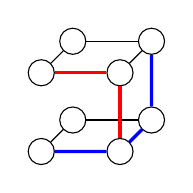
\begin{tikzpicture}
% Cube drawing with 3-arcs marked
\node[draw,circle] (0) at (0,0) {};
\node[draw,circle] (1) at (1,0) {};
\node[draw,circle] (2) at (1,1) {};
\node[draw,circle] (3) at (0,1) {};
\node[draw,circle] (4) at (0.4,0.4) {};
\node[draw,circle] (5) at (1.4,0.4) {};
\node[draw,circle] (6) at (1.4,1.4) {};
\node[draw,circle] (7) at (0.4,1.4) {};

\draw (0) -- (1) -- (2) -- (3) -- cycle;
\draw (4) -- (5) -- (6) -- (7) -- cycle;
\draw (0) -- (4);
\draw (1) -- (5);
\draw (2) -- (6);
\draw (3) -- (7);

% Mark one 3-arc in red
\draw[red,very thick] (0) -- (1) -- (2) -- (3);
% Mark another 3-arc in blue that can't be mapped to the red one
\draw[blue,very thick] (0) -- (1) -- (5) -- (6);
\end{tikzpicture}
\caption{Inequivalent 3-arcs in the cube}
\label{fig:cube-arcs}
\end{figure}

A graph $X$ is \emph{$s$-arc transitive} if it has a group $G$ of automorphisms such that $G$ is transitive, and the stabilizer $G_u$ of a vertex $u$ acts transitively on the $s$-arcs with initial vertex $u$.



\begin{theorem}
Let $X$ be a vertex-transitive graph and $s\ge 1$. Then $X$ is
$s$-arc-transitive if and only if, for any vertex $v$, the stabilizer
$\mathrm{Aut}(X)_v$ acts transitively on the set of $(s-1)$-arcs starting at $v$.

In particular, $X$ is arc-transitive (i.e., $1$-arc-transitive) if and
only if, for any vertex $v$, the stabilizer $\mathrm{Aut}(X)_v$ acts
transitively on the neighborhood of $v$.
\end{theorem}

\begin{proof}
 
\noindent \textbf{($\Rightarrow$) If $X$ is $s$-arc-transitive, then the
stabilizer acts transitively on $(s-1)$-arcs from $v$.}  

Fix a vertex $v \in V(X)$. Let $\mathcal{A}_{s-1}(v)$ denote the set of
$(s-1)$-arcs starting at $v$, i.e.,
\[
\mathcal{A}_{s-1}(v) = \{(v,v_1,\dots,v_{s-1}) : (v,v_1,\dots,v_{s-1}) \text{ is an $(s-1)$-arc}\}.
\]

Take any two $(s-1)$-arcs from $v$, say
$(v,v_1,\dots,v_{s-1})$ and $(v,u_1,\dots,u_{s-1})$. Consider
any extensions to $s$-arcs:
\[
(v,v_1,\dots,v_{s-1},v_s), \quad (v,u_1,\dots,u_{s-1},u_s)
\]
for some suitable $v_s,u_s$ so that these are $s$-arcs. Since $X$ is
$s$-arc-transitive, there exists $\phi \in \mathrm{Aut}(X)$ with
\[
\phi(v,v_1,\dots,v_{s-1},v_s) = (v,u_1,\dots,u_{s-1},u_s).
\]
Because both $s$-arcs start at $v$, it follows that $\phi$ fixes $v$,
i.e., $\phi \in \mathrm{Aut}(X)_v$. Restricting to the first $s-1$
vertices shows that $\mathrm{Aut}(X)_v$ maps $(v,v_1,\dots,v_{s-1})$ to
$(v,u_1,\dots,u_{s-1})$. Hence $\mathrm{Aut}(X)_v$ acts transitively on
$(s-1)$-arcs starting at $v$.

\medskip

\noindent \textbf{($\Leftarrow$) If the stabilizer acts transitively on
$(s-1)$-arcs from $v$, then $X$ is $s$-arc-transitive.}  

Let $(u_0,u_1,\dots,u_s)$ and $(v_0,v_1,\dots,v_s)$ be any two
$s$-arcs in $X$. Because $X$ is vertex-transitive, there exists
$\psi \in \mathrm{Aut}(X)$ with $\psi(u_0) = v_0$. Then
$(\psi(u_0),\psi(u_1),\dots,\psi(u_{s-1}))$ is an $(s-1)$-arc starting
at $v_0$. By assumption, the stabilizer $\mathrm{Aut}(X)_{v_0}$ acts
transitively on $(s-1)$-arcs from $v_0$, so there exists $\phi \in
\mathrm{Aut}(X)_{v_0}$ such that
\[
\phi(\psi(u_1),\dots,\psi(u_{s-1})) = (v_1,\dots,v_{s-1}).
\]
Then $\phi \circ \psi \in \mathrm{Aut}(X)$ maps $(u_0,\dots,u_{s-1})$ to
$(v_0,\dots,v_{s-1})$. By choosing the final vertex appropriately
(using adjacency constraints), we extend this mapping to the full
$s$-arc. Therefore $X$ is $s$-arc-transitive.

\medskip

\noindent \textbf{Special case: arc-transitive.}  

For $s=1$, a $1$-arc is just an edge $(v_0,v_1)$ with a direction. The
stabilizer $\mathrm{Aut}(X)_v$ acts transitively on the set of neighbors
of $v$ if and only if for any two edges $(v,u)$ and $(v,w)$ there exists
$\phi \in \mathrm{Aut}(X)_v$ with $\phi(u)=w$. This is exactly
$1$-arc-transitivity (arc-transitivity).

\end{proof}

\begin{lemma}
The graphs $J(v, k, i)$ are at least arc transitive.
\end{lemma}

\begin{proof}
Consider the vertex $\{1, \ldots, k\}$. The stabilizer of this vertex contains $\mathrm{Sym}(k) \times \mathrm{Sym}(v - k)$. Clearly, any two $k$-sets meeting this initial vertex in an $i$-set can be mapped to each other by this group.
\end{proof}


\begin{example}
  
Let $C_n$ be the cycle on $n$ vertices, and let $s$ be an integer with $0 \leq s \leq n-1$. 
Then $C_n$ is $s$-arc-transitive: the automorphism group $\mathrm{Aut}(C_n)\cong D_{2n}$ 
acts transitively on the set of $s$-arcs of $C_n$.
\end{example}

\begin{proof}
Model $C_n$ as the vertices $\{0,1,\dots,n-1\}$ with indices taken modulo $n$, 
where $i$ is adjacent to $i\pm 1 \pmod n$. 

An $s$-arc is an ordered sequence
\[
(v_0,v_1,\dots,v_s),
\]
where $v_i$ is adjacent to $v_{i+1}$ and $v_{i-1}\neq v_{i+1}$ for all $i$. 
On a cycle, this condition forces each step $v_{i+1}$ to be either the clockwise or 
counterclockwise neighbor of $v_i$, and since immediate backtracking is forbidden, 
each successive step continues in the same direction. 

Hence every $s$-arc is a simple directed path of length $s$ along the cycle. 
More concretely, for some start vertex $a\in\{0,\dots,n-1\}$ and for some choice of 
sign $\varepsilon\in\{+1,-1\}$ we have
\[
(v_0,v_1,\dots,v_s)=
\bigl(a,\;a+\varepsilon,\;a+2\varepsilon,\;\dots,\;a+s\varepsilon\bigr),
\]
with arithmetic modulo $n$. Thus an $s$-arc is completely determined by its starting 
vertex $a$ and its direction $\varepsilon$.

The automorphism group of the cycle is the dihedral group $D_{2n}$, generated by 
the rotation $r\colon i\mapsto i+1$ and a reflection $\rho$ (e.g.\ $\rho(i)=-i$). 
Rotations act transitively on start vertices: for any two $s$-arcs
\[
A=(a,a+\varepsilon,\dots,a+s\varepsilon),\qquad
B=(b,b+\delta,\dots,b+s\delta),
\]
the rotation $r^{\,b-a}$ sends $A$ to 
\[
r^{\,b-a}(A)=(b,b+\varepsilon,\dots,b+s\varepsilon).
\]

If $\varepsilon=\delta$, then $r^{\,b-a}$ maps $A$ to $B$. 
If $\varepsilon\neq \delta$, then compose with the reflection: 
\[
\rho\circ r^{\,b-a}(A)=(b,b-\varepsilon,\dots,b-s\varepsilon),
\]
and since $-\varepsilon=\delta$, this equals $B$.

Thus for any two $s$-arcs $A,B$ there exists an automorphism in $D_{2n}$ 
sending $A$ to $B$. Hence $C_n$ is $s$-arc-transitive for all $0\le s\le n-1$.
\end{proof}




\begin{example}
    $K_n$ is $s$-arc-transitive only for $s = 0,1,2$.
\end{example}

\begin{example}
    Cube $Q_3$ is $2$-arc-transitive but not $3$-arc-transitive.
\end{example}

\begin{proof}
Model \(Q_3\) as the graph with vertex set \(\{0,1\}^3\) (binary
3-tuples). Two vertices are adjacent iff they differ in exactly one
coordinate. The automorphism group of \(Q_3\) contains all coordinate
permutations and all independent bit-flips, so in particular it preserves
Hamming distance between vertices.

\medskip\noindent\textbf{(1) $Q_3$ is $2$-arc-transitive.}  
Fix a vertex, say \(v_0=(0,0,0)\). Its neighbors are the three unit
vectors \(e_1=(1,0,0), e_2=(0,1,0), e_3=(0,0,1)\). Any 2-arc starting at
\(v_0\) is of the form \((v_0,e_i,e_j)\) with \(i\neq j\) (the
non-backtracking condition forbids \(i=j\)). The stabilizer of \(v_0\)
inside \(\operatorname{Aut}(Q_3)\) contains the full permutation group
on the three coordinates, i.e.\ a copy of \(S_3\). This \(S_3\)-action
permutes \(\{e_1,e_2,e_3\}\) arbitrarily, hence acts transitively on
ordered pairs \((e_i,e_j)\) with \(i\neq j\). Therefore the stabilizer
of \(v_0\) acts transitively on the set of 2-arcs starting at \(v_0\).
Since the cube is vertex-transitive, this implies \(\operatorname{Aut}(Q_3)\)
is transitive on all 2-arcs, i.e.\ \(Q_3\) is 2-arc-transitive.

\medskip\noindent\textbf{(2) $Q_3$ is not $3$-arc-transitive.}  
Consider 3-arcs, i.e. ordered non-backtracking paths of length 3
\((v_0,v_1,v_2,v_3)\). The automorphism group preserves Hamming distances,
so the Hamming distance \(d(v_0,v_3)\) is an invariant of the orbit of
a 3-arc. We show there exist 3-arcs with different values of
\(d(v_0,v_3)\), hence there are at least two distinct orbits of
3-arcs, so the action is not transitive on 3-arcs.

Example 1 (distance \(3\)). Take the path
\[
(000,100,110,111).
\]
Here \(v_0=000\) and \(v_3=111\), so \(d(v_0,v_3)=3\).

Example 2 (distance \(1\)). Take the path
\[
(000,100,101,001).
\]
Here \(v_0=000\) and \(v_3=001\), so \(d(v_0,v_3)=1\).

Both sequences are valid non-backtracking paths of length \(3\) in
\(Q_3\). Because \(d(v_0,v_3)\) is preserved by every graph automorphism,
no automorphism can send the first 3-arc to the second. Hence the set
of all 3-arcs splits into at least two orbits under
\(\operatorname{Aut}(Q_3)\), so \(Q_3\) is not 3-arc-transitive.

Combining (1) and (2) proves the theorem.
\end{proof}


\bigskip\noindent\textbf{Exercise}
    Let $\Gamma$ be a graph with minimum degree at least 2. Then $\Gamma$ is $(s + 1)$-arc-transitive if and only if $\Gamma$ is $s$-arc-transitive and the stabilizer in $\text{Aut}(\Gamma)$ of any $s$-arc $(v_0, \dots, v_{s-1}, v_s)$ acts transitively on $\Gamma(v_s) \setminus \{v_{s-1}\}$.


\begin{example}
    Petersen graph is $3$-arc-transitive but not $4$-arc-transitive.
\end{example}


\begin{proof}
We prove both statements separately.

\medskip

\textbf{Part 1: $3$-arc-transitivity}

Let $P$ denote the Petersen graph. We establish $3$-arc-transitivity through these steps:

\begin{enumerate}
    \item The automorphism group $\operatorname{Aut}(P)$ is isomorphic to $S_5$ and has order $120$.

    \item $P$ is arc-transitive.
    
    \item $P$ has $15$ undirected edges and $30$ directed arcs (each edge gives two arcs)
    \item For any arc $(u,v) \in V \times V$ with $u \sim v$, the arc stabilizer is:
\[ G_{(u,v)} = G_u \cap G_v \] where $G_u$ and $G_v$ are the vertex stabilizers, $V=V(P)$

\item $G_u \cong D_6$ (dihedral group of order 12)
        
        \item $G_u \cap G_v \cong \mathbb{Z}_2$ when $u \sim v$, So $G_u$ is transitive on 2-arcs initiate from $u$, which implies that $P$ is 2-arc transitive.
        \item $P$ has 60 2-arcs, so  for any $2$-arc $(u,v,w)$, the stabilizer in $\operatorname{Aut}(\mathcal{P})$ is ismorphic to $\mathbb{Z}_2$ and  acts transitively on the remaining neighbors of $w$ (excluding $v$). This follows because:
    
        \item The neighborhood of any vertex induces a matching (no two neighbors are adjacent)
        \item The stabilizer of a $2$-arc has order $2$ and can swap the remaining two neighbors
    
    
    

    \item So $P$ is 3-arc transitive.
    
    \item $P$ has 120 3-arcs and so the pointwise stabilizer of a $3$-arc is trivial which implies that it is not 4-arc transtive
    
\end{enumerate}



Thus while $\operatorname{Aut}(P)$ acts transitively on $3$-arcs, it has two distinct orbits on $4$-arcs.
\end{proof}








\begin{theorem}
For every integer $k\ge 1$ the graph $J(2k+1,k,0)$ (the odd graph $O_k$)
is $2$-arc-transitive: its automorphism group acts transitively on the
set of directed paths of length $2$ (i.e. on ordered triples
$(A,B,C)$ with $A\!-\!B\!-\!C$ an $2$-arc).
\end{theorem}

\begin{proof}
Model $J(2k+1,k,0)$ as follows. Let $\Omega$ be a fixed set with
$|\Omega|=2k+1$. Vertices of the graph are the $k$-subsets of $\Omega$.
Two vertices (subsets) are adjacent iff they are disjoint. The symmetric
group $S_{\Omega}\cong S_{2k+1}$ acts naturally on the vertex set by
permuting elements of $\Omega$, and this action preserves disjointness;
hence $S_{\Omega}\le \mathrm{Aut}(J(2k+1,k,0))$. Thus it suffices to
show that $S_{\Omega}$ acts transitively on the set of directed paths of
length $2$.

Let $(A,B,C)$ be any directed path of length \(2\); that is
\(A,B,C\) are \(k\)-subsets of \(\Omega\) with \(A\cap B=\varnothing\),
\(B\cap C=\varnothing\), and \(A\neq C\) (the non-backtracking
condition). From the disjointness conditions we obtain the crucial
constraint on \(|A\cap C|\). Indeed
\[
B\subseteq \Omega\setminus(A\cup C),
\]
so
\[
k = |B| \le |\Omega\setminus(A\cup C)| = (2k+1) - |A\cup C|.
\]
But $|A\cup C| = |A|+|C|-|A\cap C| = 2k-|A\cap C|$, so the previous
inequality becomes
\[
k \le (2k+1) - (2k-|A\cap C|) = 1 + |A\cap C|,
\]
hence \(|A\cap C|\ge k-1\). Since \(|A\cap C| \le k\) and equality
\(|A\cap C|=k\) would force \(A=C\) (forbidden), we must have
\[
|A\cap C| = k-1.
\]
Thus every directed 2-path \((A,B,C)\) in the odd graph satisfies
\(|A\cap C|=k-1\).

Now fix a convenient canonical 2-arc:
\[
A_0=\{1,2,\dots,k\},\qquad B_0=\{k+1,k+2,\dots,2k\},\qquad
C_0=\{1,2,\dots,k-1,2k+1\},
\]
where $\Omega=\{1,2,\dots,2k+1\}$. Note that $A_0\cap B_0=\varnothing$,
$B_0\cap C_0=\varnothing$, and $|A_0\cap C_0|=k-1$, so $(A_0,B_0,C_0)$ is
indeed a directed 2-path.

We claim any directed 2-path \((A,B,C)\) can be sent to
\((A_0,B_0,C_0)\) by some permutation in \(S_{\Omega}\). To see this,
choose an enumeration of the elements of \(A\) and \(C\) so that the
first \(k-1\) elements are the common elements of \(A\cap C\). Using a
permutation we may send those \(k-1\) common elements to
\(\{1,2,\dots,k-1\}\), the unique element in \(A\setminus C\) to \(k\),
and the unique element in \(C\setminus A\) to \(2k+1\). Finally send the
\(k\) elements of \(B\) (which lie in the complement of \(A\cup C\), a
set of size \(k\)) to \(\{k+1,\dots,2k\}\). This defines a bijection of
\(\Omega\) sending \((A,B,C)\) to \((A_0,B_0,C_0)\). Thus every directed
2-path lies in the same orbit of \(S_{\Omega}\).

Since $S_{\Omega}\le\mathrm{Aut}(J(2k+1,k,0))$, the full automorphism
group is transitive on directed 2-paths; i.e.\ the graph is
$2$-arc-transitive.
\end{proof}



The \emph{girth} of a graph is the length of the shortest cycle in it. Our first result implies that the subgraphs induced by $s$-arcs in $s$-arc transitive graphs are paths.

\begin{theorem}[Tutte]
If $X$ is an $s$-arc transitive graph with valency at least three and girth $g$, then $g \geq 2s - 2$.
\end{theorem}

\begin{proof}
We may assume that $s \geq 3$, since the condition on the girth is otherwise meaningless. It is easy to see that $X$ contains a cycle of length $g$ and a path of length $g$ whose end-vertices are not adjacent. Therefore $X$ contains a $g$-arc with adjacent end-vertices and a $g$-arc with nonadjacent end-vertices; clearly, no automorphism can map one to the other, and so $s < g$. 

Since $X$ contains cycles of length $g$, and since these contain $s$-arcs, it follows that any $s$-arc must lie in a cycle of length $g$. Suppose that $v_0, \ldots, v_s$ is an $s$-arc. Denote it by $\Delta$. Since $v_{s-1}$ has valency at least three, it is adjacent to a vertex $w$ other than $v_{s-2}$ and $v_s$, and since the girth of $X$ is at least $s$, this vertex cannot lie in $\Delta$. Hence we may replace $v_s$ by $w$, obtaining a second $s$-arc $\beta$ that intersects $\Delta$ in an $(s-1)$-arc. Since $\beta$ must lie in a circuit of length $g$, we thus obtain a pair of circuits of length $g$ that have at least $s - 1$ edges in common.

If we delete these $s - 1$ edges from the graph formed by the edges of the two circuits of length $g$, the resulting graph still contains a cycle of length at most $2g - 2s + 2$. Hence $2g - 2s + 2 \geq g$, and the result follows.
\end{proof}

Given this lemma, it is natural to ask what can be said about the $s$-arc transitive graphs with girth $2s - 2$. It follows from our next result that these graphs are, in the language ofnext chapter, generalized polygons. It is a consequence of results we state there that $s \leq 9$.

\begin{theorem}[Tutte]
If $X$ is an $s$-arc transitive graph with girth $2s - 2$, it is bipartite and has diameter $s - 1$.
\end{theorem}

\begin{proof}
We first observe that if $X$ has girth $2s - 2$, then any $s$-arc lies in at most one cycle of length $2s - 2$, and so if $X$ is $s$-arc transitive, it follows that every $s$-arc lies in a unique cycle of length $2s - 2$. Clearly, $X$ has diameter at least $s - 1$, because opposite vertices in a cycle of length $2s - 2$ are at this distance. 

Now, let $u$ be a vertex of $X$ and suppose for a contradiction that $v$ is a vertex at distance $s$ from it. Then there is an $s$-arc joining $u$ to $v$, which must lie in a cycle of length $2s - 2$. Since a cycle of this length has diameter $s - 1$, it follows that $v$ cannot be of distance $s$ from $u$. Therefore, the diameter of $X$ is at most $s - 1$ and hence equal to $s - 1$.

If $X$ is not bipartite, then it contains an odd cycle; suppose $C$ is an odd cycle of minimal length. Because the diameter of $X$ is $s-1$, the cycle must have length $2s - 1$. Let $u$ be a vertex of $C$, and let $v$ and $v'$ be the two adjacent vertices in $C$ at distance $s - 1$ from $u$. Then we can form an $s$-arc $(u, \ldots, v, v')$. This $s$-arc lies in a cycle $C'$ of length $2s - 2$. The vertices of $C$ and $C'$ not internal to the $s$-arc form a cycle of length less than $2s - 2$, which is a contradiction.
\end{proof}

We will use this lemma to show that $s$-arc transitive graphs with girth $2s - 2$ are distance transitive.


\noindent\textbf{Arc Graphs}

If $s \geq 1$ and $\alpha = (x_0, \dots, x_s)$ is an arc in $X$, we define its \emph{head} $\text{head}(\alpha)$ 
to be the $(s - 1)$-arc $(x_1, \dots, x_s)$ and its \emph{tail} $\text{tail}(\alpha)$ to be the $(s - 1)$-arc 
$(x_0, \dots, x_{s-1})$. If $\alpha$ and $\beta$ are $s$-arcs, then we say that $\beta$ \emph{follows} $\alpha$ if there 
is an $(s+1)$-arc $\gamma$ such that $\text{head}(\gamma) = \beta$ and $\text{tail}(\gamma) = \alpha$. (Somewhat more 
colourfully, we say that $\alpha$ can be \emph{shunted} onto $\beta$, and envisage pushing $\alpha$ 
one step onto $\beta$.) Let $s$ be a nonnegative integer. We use $X^{(s)}$ to denote 
the directed graph with the $s$-arcs of $X$ as its vertices, such that $(\alpha, \beta)$ is 
an arc if and only if $\alpha$ can be shunted onto $\beta$. Any automorphisms of $X$ 
extend naturally to automorphisms of $X^{(s)}$, and so if $X$ is $s$-arc transitive, 
then $X^{(s)}$ is vertex transitive.

\begin{lemma}
Let $X$ and $Y$ be directed graphs and let $f$ be a homomorphism from $X$ onto $Y$ such that every edge in $Y$ is the image of an edge in $X$. Suppose $y_0, \dots, y_r$ is a path in $Y$. Then for each vertex $x_0$ in $X$ such that $f(x_0) = y_0$, there is a path $x_0, \dots, x_r$ such that $f(x_i) = y_i$.
\end{lemma}

\begin{proof}
Exercise.
\end{proof}

\section{ s-arc Transitive Graphs}

Define a \emph{spindle} in $X$ to be a subgraph consisting of two given vertices joined by three paths, with any two of these paths having only the given vertices in common. Define a \emph{bicycle} to be a subgraph consisting either of two cycles with exactly one vertex in common, or two vertex-disjoint cycles and a path joining them having only its end-vertices in common with the cycles. We claim that if $X$ is a spindle or a bicycle, then $X^{(1)}$ is strongly connected. We leave the proof of this as an easy exercise. Nonetheless, it is the key to the proof of the following result.

\begin{theorem}
If $X$ is a connected graph with minimum valency two that is not a cycle, then $X^{(s)}$ is strongly connected for all $s \geq 0$.
\end{theorem}

\begin{proof}
First we shall prove the result for $s = 0$ and $s = 1$, and then by induction on $s$. If $s = 0$, then $X^{(0)}$ is the graph obtained by replacing each edge of $X$ with a pair of oppositely directed arcs, so the result is clearly true. If $s = 1$, then we must show that any $1$-arc can be shunted onto any other $1$-arc. Since $X$ is connected, we can shunt any $1$-arc onto any edge of $X$, but not necessarily facing in the right direction. Therefore, it is necessary and sufficient to show that we can reverse the direction of any $1$-arc, that is, shunt $xy$ onto $yx$.

Since $X$ has minimum valency at least two and is finite, it contains a cycle, $C$ say. If $C$ does not contain both $x$ and $y$, then there is a (possibly empty) path in $X$ joining $y$ to $C$. It is now easy to shunt $xy$ along the path, around $C$, then back along the path in the opposite direction to $yx$.

If $x$ and $y$ are in $V(C)$ but $xy \notin E(C)$, then $C$ together with the edge $xy$ is a spindle, and we are done.

Hence we may assume that $xy \in E(C)$. Since $X$ is not a cycle, there is a vertex in $C$ adjacent to a vertex not in $C$. Suppose $w$ in $V(C)$ is adjacent to a vertex $z$ not in $C$. Let $P$ be a path with maximal length in $X$, starting with $w$ and $z$, in this order. Then the last vertex of $P$ is adjacent to a vertex in $P$ or a vertex in $C$. If it is adjacent to a vertex in $C$ other than $w$, then $xy$ is an edge in a spindle. If it is adjacent to $w$ or to a vertex of $P$ not in $C$, then $xy$ is an edge in a bicycle. In either case we are done.

Now, assume that $X^{(s)}$ is strongly connected for some $s \geq 1$. It is easy to see that the operation of taking the head of an $(s + 1)$-arc is a homomorphism from $X^{(s+1)}$ to $X^{(s)}$. Since $X$ has minimum valency at least two, each $s$-arc is the head of an $(s + 1)$-arc, and it follows that every edge of $X^{(s)}$ is the image of an edge in $X^{(s+1)}$. Let $\alpha$ and $\beta$ be any two $(s+1)$-arcs in $X$. Since $X^{(s)}$ is strongly connected, there is a path in it joining $\text{head}(\alpha)$ to $\text{tail}(\beta)$. By the lemma above, this path lifts to a path in $X^{(s+1)}$ from $\alpha$ to a vertex, where $\text{head}(\gamma) = \text{tail}(\beta)$. Since $s \geq 1$ and $X$ has minimum valency at least two, we see that $\gamma$ can be shunted onto $\beta$. Thus $\alpha$ can be shunted to $\beta$ via $\gamma$, and so there is a path in $X^{(s+1)}$ from $\alpha$ to $\beta$.
\end{proof}

\section{ Cubic s-arc Transitive Graphs}

In 1947 Tutte showed that for any $s$-arc transitive cubic graph, $s \leq 5$. This was, eventually, the stimulus for a lot of work. One outcome of this was a proof, by Richard Weiss, that for any $s$-arc transitive graph, $s \leq 7$. This is a very deep result, the proof of which depends on the classification of the finite simple groups.



\begin{lemma}
Let $X$ be a strongly connected directed graph, let $G$ be a transitive subgroup of its automorphism group, and, if $u \in V(X)$, let $N(u)$ be the set of vertices $v$ in $V(X)$ such that $(u, v)$ is an arc of $X$. If there is a vertex $u$ of $X$ such that $G_u \cap N(u)$ is the identity, then $G$ is regular.
\end{lemma}

\begin{proof}
Suppose $u \in V(X)$ and $G_u \cap N(u)$ is the identity group. If $v \in V(X)$, then $G_v$ is conjugate in $G$ to $G_u$. Hence $G_v \cap N(v)$ must be the identity for all vertices $v$ of $X$.

Assume, by way of contradiction, that $G_u$ is not the identity group. Since $X$ is strongly connected, we may choose a directed path that goes from $u$ to a vertex, $w$ say, that is not fixed by $G_u$. Choose this path to have minimum possible length, and let $v$ denote the second-last vertex on it. Thus $v$ is fixed by $G_u$, and $(v, w)$ is an arc in $X$. Since $G_u$ fixes all vertices in $N(u)$, we see that $v \neq u$.

Since $G_u$ fixes $v$, it fixes $N(v)$ but acts nontrivially on it, because it does not fix $w$. Hence $G_v \cap N(v)$ is not the identity. This contradiction forces us to conclude that $G_u = (e)$.
\end{proof}

A graph is \emph{$s$-arc regular} if for any two $s$-arcs there is a unique automorphism mapping the first to the second.

\begin{lemma}
Let $X$ be a connected cubic graph that is $s$-arc transitive, but not $(s + 1)$-arc transitive. Then $X$ is $s$-arc regular.
\end{lemma}

\begin{proof}
We note that if $X$ is cubic, then $X^{(s)}$ has out-valency two. Now let $G$ be the automorphism group of $X$, let $\alpha$ be an $s$-arc in $X$, and let $H$ be the subgroup of $G$ fixing each vertex in $\alpha$. Then $G$ acts vertex transitively on $X^{(s)}$, and $H$ is the stabilizer in $G$ of the vertex $\alpha$ in $X^{(s)}$. If the restriction of $H$ to the out-neighbours of $\alpha$ is not trivial, then $H$ must swap the two $s$-arcs that follow $\alpha$. Now, any two $(s + 1)$-arcs in $X$ can be mapped by elements of $G$ to $(s + 1)$-arcs that have $\alpha$ as the "initial" $s$-arc; hence in this case we see that $G$ is transitive on the $(s + 1)$-arcs of $X$, which contradicts our initial assumption.

Hence the restriction of $H$ to the out-neighbours of $\alpha$ is trivial, and it follows  that $H$ itself is trivial. Therefore, we have proved that $G_\alpha = (e)$, and so $G$ acts regularly on the $s$-arcs of $X$.
\end{proof}

If $X$ is a regular graph with valency $k$ on $n$ vertices and $s \geq 1$, then there are exactly $nk(k - 1)^{s-1}$ $s$-arcs. It follows that if $X$ is $s$-arc transitive then $|\text{Aut}(X)|$ must be divisible by $nk(k - 1)^{s-1}$, and if $X$ is $s$-arc regular, then $|\text{Aut}(X)| = nk(k - 1)^{s-1}$. In particular, a cubic arc-transitive graph $X$ is $s$-arc regular if and only if 
\[
|\text{Aut}(X)| = (3n)2^{s-1}.
\]
For an example, consider the cube. It is clear that the stabilizer of a vertex contains $\text{Sym}(3)$, and therefore its automorphism group has size at least 48. We observed earlier that the cube is not $3$-arc transitive, so  it must be precisely $2$-arc regular, with full automorphism group of order 48.



Finally, we state Tutte's theorem.

\begin{theorem}
If $X$ is an $s$-arc regular cubic graph, then $s \leq 5$.
\end{theorem}

\begin{proof}
Let $X$ be a connected cubic graph with $n$ vertices, and let $G = \mathrm{Aut}(X)$. Suppose $X$ is \emph{$s$-arc-regular}, meaning $G$ acts regularly on the set of $s$-arcs of $X$ (an $s$-arc is a sequence $(v_0,v_1,\dots,v_s)$ of $s+1$ vertices such that $v_i$ is adjacent to $v_{i+1}$ and $v_{i-1}\ne v_{i+1}$ for $1\le i\le s-1$).  

\medskip
\textbf{Step 1: Counting $s$-arcs and the group order.}  

For a cubic graph:
\begin{itemize}
    \item Each vertex $v$ has 3 neighbors.
    \item Starting from $v_0$, there are 3 choices for $v_1$.
    \item For each subsequent step $i\ge 2$, there are 2 choices for $v_i$ (avoiding the previous vertex to prevent backtracking).
\end{itemize}
Hence the number of $s$-arcs is
\[
\#\{\text{$s$-arcs}\} = n \cdot 3 \cdot 2^{s-1}.
\]
Since $G$ acts regularly on $s$-arcs, the order of $G$ equals the number of $s$-arcs:
\[
|G| = n \cdot 3 \cdot 2^{s-1}.
\]

Let $v\in V(X)$, and let $G_v$ denote the stabilizer of $v$ in $G$. By the orbit-stabilizer theorem:
\[
|G| = n \cdot |G_v| \implies |G_v| = 3 \cdot 2^{s-1}.
\]

\medskip
\textbf{Step 2: Local action at a vertex.}  

Since $X$ is arc-transitive, $G_v$ acts transitively on the 3 neighbors of $v$. Therefore $G_v$ embeds as a transitive subgroup of $\mathrm{Sym}(3)$
implying:
\[
3 \mid |G_v|.
\]

The stabilizer of an arc $(v,u)$, i.e.\ $G_{(v,u)}$, is the subgroup of $G_v$ fixing $u$:
\[
|G_{(v,u)}| = \frac{|G_v|}{3} = 2^{s-1}.
\]

\medskip
\textbf{Step 3: Growth constraints for $s$-arc-regularity.}  

Consider the faithful action of $G_v$ on all $s$-arcs starting at $v$. Each extension of an arc from $v$ multiplies the number of possible continuations by 2 (except the backtracking edge). Therefore:
\begin{itemize}
    \item $|G_v| = 3\cdot 2^{s-1}$ grows exponentially in $s$.
    \item To preserve the $s$-arc structure faithfully, $G_v$ must act effectively on $2^{s-1}$ different possible sequences.
\end{itemize}

\medskip
\textbf{Step 4: Why $s \ge 6$ fails.}  

If $s \ge 6$:
\begin{enumerate}
    \item $|G_v| = 3 \cdot 2^{s-1} \ge 96$.
    \item $G_v$ must permute $2^{s-1}\ge32$ possible continuation sequences for arcs of length $s$.
    \item A cubic graph only allows 2 forward choices at each step, so the structure of $s$-arcs restricts the action.
    \item Maintaining faithful $s$-arc-regularity forces the automorphism to also preserve $(s+1)$-arcs, which is impossible if $s$ is maximal.
\end{enumerate}
Hence no cubic $s$-arc-regular graph exists for $s \ge 6$.

\medskip
\textbf{Step 5: Geometric intuition.}  

At each vertex $v$, the three incident edges consist of:
\begin{itemize}
    \item one edge back to the previous vertex,
    \item two edges leading forward along potential $s$-arcs.
\end{itemize}
For large $s$, the automorphism must distinguish increasingly many forward paths. Eventually, the local action of $G_v$ cannot accommodate all constraints without affecting longer arcs, forcing a violation of $s$-arc regularity.

\medskip
\textbf{Step 6: Maximum case and example.}  

For $s=5$, the numbers work out:
\[
|G_v| = 3 \cdot 2^4 = 48,
\]
and Tutte’s $8$-cage on $30$ vertices realizes this maximum. The full automorphism group has order:
\[
|G| = 30 \cdot 48 = 1440.
\]

\medskip
\textbf{Conclusion.}  

Therefore, for cubic $s$-arc-regular graphs:
\[
s \le 5.
\]
\end{proof}

\begin{corollary}
Let $X$ be an arc-transitive cubic graph with automorphism group $G$ and vertex stabilizer $G_v$. Then:
\[
|G_v| \mid 48 \quad \text{and} \quad 3 \mid |G_v|.
\]
\end{corollary}

\begin{proof}
From the proof above, the maximal vertex stabilizer occurs at $s=5$, giving $|G_v| = 48$, divisible by 3 due to the required transitivity on the 3 neighbors of $v$. Smaller $s$ give smaller divisors of 48.
\end{proof}



The smallest $5$-arc regular cubic graph is Tutte's $8$-cage on $30$ vertices.

\begin{corollary}[4.3.4]
If $X$ is an arc-transitive cubic graph, $v \in V(X)$, and $G = \text{Aut}(X)$, then $|G_v|$ divides $48$ and is divisible by three.
\end{corollary}

\begin{theorem}[Weiss, 1981; refined version]
Let $X$ be a finite connected $k$-regular graph, and suppose that $X$ is $s$-arc-transitive
(i.e., its automorphism group acts transitively on the set of $s$-arcs). Then:
\[
s \le 7.
\]

Moreover, equality $s=7$ occurs only for graphs of very special structure:
\begin{itemize}
    \item The graph must satisfy highly restrictive combinatorial and group-theoretic conditions.
    \item Such graphs are extremely rare and require special constructions.
\end{itemize}
\end{theorem}

\noindent\textbf{Remark:}
\begin{itemize}
    \item This result generalizes Tutte's theorem for cubic graphs, which is the case $k=3$, where the maximal $s$ is $5$.
    \item The Weiss theorem shows that no matter the valency, the $s$-arc-transitive property cannot extend indefinitely; there is an absolute upper bound of $7$.
    \item The bound $s\le 7$ is sharp in the sense that there do exist graphs realizing $s=7$, but they are exceptional.
\end{itemize}


\begin{corollary}[Vertex stabilizers in cubic $s$-arc-regular graphs, Tutte]
Let $X$ be a connected cubic $s$-arc-regular graph with $s \le 5$, and let $v \in V(X)$.  
Let $G_v = \mathrm{Stab}_{\mathrm{Aut}(X)}(v)$ denote the vertex stabilizer. Then
\[
|G_v| = 3 \cdot 2^{s-1},
\]
and the group structure is:

\begin{enumerate}
    \item $s=1$: $|G_v| = 3$, \quad $G_v \cong C_3$.
    \item $s=2$: $|G_v| = 6$, \quad $G_v \cong S_3$.
    \item $s=3$: $|G_v| = 12$, \quad $G_v \cong C_2 \times S_3$ (the 3-cycle acts faithfully on the 3 neighbors).
    \item $s=4$: $|G_v| = 24$, \quad $G_v \cong S_4$.
    \item $s=5$: $|G_v| = 48$, \quad $G_v \cong C_2 \times S_4$ (realized in Tutte's 8-cage).
\end{enumerate}
\end{corollary}

\begin{proof}
Let $X$ be a connected cubic $s$-arc-regular graph with automorphism group $G = \mathrm{Aut}(X)$.

\medskip
\textbf{Step 1: Counting $s$-arcs.}  
At each vertex, there are 3 neighbors. Beyond the first step, each step along an $s$-arc has 2 choices (to avoid backtracking).  
Hence, the number of $s$-arcs starting at a fixed vertex $v$ is
\[
3 \cdot 2^{s-1}.
\]
Since $G$ acts regularly on the set of $s$-arcs, the orbit-stabilizer theorem gives
\[
|G_v| = 3 \cdot 2^{s-1}.
\]

\medskip
\textbf{Step 2: Determining the structure.}  

\begin{itemize}
    \item $s=1$: $G_v$ acts transitively on the 3 neighbors and has no further choices, so $G_v \cong C_3$.
    
    \item $s=2$: $G_v$ permutes the 3 neighbors and acts on the 2-step extensions. This gives a group of order 6, which must be $S_3$.
    
    \item $s=3$: $G_v$ has order 12. There is a normal subgroup of order 2 corresponding to the binary choice along one step of the 3-arc, and the quotient of order 6 is $S_3$ acting faithfully on neighbors. Hence $G_v \cong C_2 \times S_3$.
    
    \item $s=4$: $G_v$ has order 24. Its Sylow 2-subgroup of order 8 corresponds to the normal 2-group acting on the first 3 steps, and the subgroup of order 3 acts transitively on the neighbors. By group-theoretic classification, the only nonabelian group of order 24 with these properties is $S_4$. Hence $G_v \cong S_4$.
    
    \item $s=5$: $G_v$ has order 48. In Tutte's 8-cage, the 16-element 2-group is normal, and the quotient of order 3 acts transitively on neighbors. Thus, $G_v \cong C_2 \times S_4$.
\end{itemize}

\medskip
\textbf{Step 3: Verification.}  
In each case, the stabilizer acts faithfully on $s$-arcs starting at $v$, and the structures listed match both the order and the local permutation requirements. Special cases \(s=4\) and \(s=5\) correspond to $S_4$ and $C_2 \times S_4$ as noted in Tutte’s classification.
\end{proof}


\chapter{Distance-transitive  and Moore graphs}

\begin{definition}
A connected graph is \emph{distance-transitive} if given any two ordered pairs of vertices $(u, u')$ and $(v, v')$ such that $d(u, u') = d(v, v')$, there is an automorphism of $\Gamma$ such that $(v, v') = \sigma(u, u')$.
\end{definition}

\begin{example}
The complete graph $K_n$ is distance-transitive.
\end{example}

\begin{lemma}
(The Johnson graphs are distance-transitive.)
Let $v,k$ be integers with $0<k<v$. The Johnson graph $J(v,k,k-1)$
(the usual Johnson graph $J(v,k)$) is distance-transitive.
\end{lemma}

\begin{proof}
Vertices of $J(v,k,k-1)$ are the $k$-subsets of a fixed $v$-set
$\Omega=\{1,\dots,v\}$. Two vertices (subsets) $A,B$ are adjacent iff
$|A\cap B|=k-1$ (equivalently $B$ is obtained from $A$ by replacing one
element by another).

\textbf{Distance formula.} Let $A,B$ be $k$-subsets and set
$t=|A\cap B|$. We claim
\[
\mathrm{dist}(A,B)=k-t.
\]
Indeed, starting from $A$ we can replace one element at a time of
$A\setminus B$ by a distinct element of $B\setminus A$; each replacement
gives an adjacent $k$-set and after exactly $|A\setminus B|=k-t$
replacements we reach $B$. Hence $\mathrm{dist}(A,B)\le k-t$.

Conversely, along any path of length $r$ from $A$ to $B$ each step can
change the intersection with $B$ by at most one (you can gain at most
one element of $B$ at each step), so after $r$ steps the intersection
size with $B$ is at least $t+r-k$; comparing endpoints shows $r\ge k-t$.
Thus $\mathrm{dist}(A,B)=k-t$.

\textbf{Distance-transitivity.} The symmetric group $S_\Omega\cong S_v$
acts naturally on $k$-subsets and preserves intersection sizes, hence
preserves distances. Moreover, for any two ordered pairs of $k$-subsets
\((A,B)\) and \((A',B')\) with \(|A\cap B|=|A'\cap B'|\) there exists
\(\sigma\in S_\Omega\) with \(\sigma(A)=A'\) and \(\sigma(B)=B'\)
(because one can first map \(A\) to \(A'\) and then permute the remaining
elements inside complements to map \(B\) to \(B'\); this is standard and
depends only on matching the intersection pattern). Therefore
$S_\Omega\le\operatorname{Aut}(J(v,k,k-1))$ acts transitively on ordered
pairs of vertices at a given distance. That is exactly the definition of
distance-transitive. Hence $J(v,k,k-1)$ is distance-transitive.
\end{proof}

\begin{lemma}\label{lem:odd-distance-transitive}
For every integer $k \ge 1$, the graph $J(2k+1,k,0)$ (the odd graph $O_k$) is
distance-transitive.
\end{lemma}

\begin{proof}
Let $\Omega$ be a fixed set with $|\Omega| = 2k+1$. The vertices of $J(2k+1,k,0)$
are the $k$-subsets of $\Omega$, and two vertices $A,B$ are adjacent if and only if
\[
A \cap B = \varnothing .
\]

\medskip
\noindent
\textbf{Distance formula.}
Let $A,B$ be vertices and put $t = |A \cap B|$.
Then the distance between $A$ and $B$ in $O_k$ is given by
\[
\text{dist}(A,B) =
\begin{cases}
k - t, & \text{if $t$ is even},\\[4pt]
k - t + 1, & \text{if $t$ is odd}.
\end{cases}
\]
In particular, the diameter of $O_k$ is $k$, and the intersection size uniquely
determines the distance.

To see this, note that if $A_0, A_1, \dots, A_m$ is a path in $O_k$, then
$A_{i+1} \subseteq \Omega \setminus A_i$, where $|\Omega \setminus A_i| = k+1$.
Tracking the size of $A_i \cap B$ along such a path shows that the intersection
size can increase by at most one every two steps, and parity considerations force
the above formula. A constructive argument shows that these bounds are attained,
so the formula is exact.

\medskip
\noindent
\textbf{Distance-transitivity.}
The symmetric group $S_\Omega$ acts naturally on the set of $k$-subsets of $\Omega$
and preserves intersection sizes, hence distances.
Moreover, $S_\Omega$ is transitive on ordered pairs of $k$-subsets having a fixed
intersection size $t$.
Therefore $S_\Omega \le \Aut(O_k)$ acts transitively on ordered pairs of vertices
at each distance. Hence the odd graph $O_k = J(2k+1,k,0)$ is distance-transitive.
\end{proof}


For a connected graph $\Gamma$ and a vertex $v \in V(\Gamma)$, let $\Gamma_i(v)$ be the set of vertices at distance $i$ from $v$, that is $\Gamma_i(v) = \{u \in V(\Gamma) \mid d(u, v) = i\}$. Observe that for any connected graph $\Gamma$ with diameter $d$, we have that $V(\Gamma)$ is partitioned into sets $\Gamma_0(v), \Gamma_1(v), \dots, \Gamma_d(v)$. The following theorem gives a characterization of distance-transitive graphs, based on the action of the automorphism group on sets $\Gamma_i(v)$. This partition is called the \emph{distance-partition} of $\Gamma$.

\begin{theorem}
Let $\Gamma$ be a connected graph. Then $\Gamma$ is distance-transitive if and only if the following conditions hold:
\begin{enumerate}
    \item $\Gamma$ is vertex-transitive;
    \item $\text{Aut}(\Gamma)_v$ acts transitively on each of the sets $\Gamma_i(v)$ ($i = 1, \dots, \text{diam}(\Gamma)$), for any vertex $v \in V(\Gamma)$.
\end{enumerate}
\end{theorem}

\begin{proof}
($\Rightarrow$) Assume $\Gamma$ is distance-transitive.  

First, set $x_1=x_2$ and let $y_1,y_2$ be any two vertices with
$d(x_1,y_1)=d(x_2,y_2)$. By distance-transitivity there is an automorphism
$\varphi$ with $\varphi(x_1)=x_2$ and $\varphi(y_1)=y_2$. Taking $x_1$
arbitrarily shows that $\mathrm{Aut}(\Gamma)$ acts transitively on
vertices, so $\Gamma$ is vertex-transitive.

Next fix $v\in V(\Gamma)$ and an index $i$. Let $u_1,u_2\in\Gamma_i(v)$,
so $d(v,u_1)=d(v,u_2)=i$. By distance-transitivity (applied to the pairs
$(v,u_1)$ and $(v,u_2)$) there exists $\psi\in\mathrm{Aut}(\Gamma)$ with
$\psi(v)=v$ and $\psi(u_1)=u_2$. Hence $\psi\in\mathrm{Aut}(\Gamma)_v$
and the stabilizer of $v$ acts transitively on $\Gamma_i(v)$. This
verifies (2).

($\Leftarrow$) Conversely, assume (1) and (2) hold. Let
$x_1,y_1,x_2,y_2\in V(\Gamma)$ satisfy
$d(x_1,y_1)=d(x_2,y_2)=k$. By vertex-transitivity there exists
$\alpha\in\mathrm{Aut}(\Gamma)$ with $\alpha(x_1)=x_2$. Then
$d(x_2,\alpha(y_1))=d(x_1,y_1)=k$, so $\alpha(y_1)\in\Gamma_k(x_2)$.
By hypothesis (2) the stabilizer $\mathrm{Aut}(\Gamma)_{x_2}$ acts
transitively on $\Gamma_k(x_2)$, hence there exists
$\beta\in\mathrm{Aut}(\Gamma)_{x_2}$ with
$\beta(\alpha(y_1))=y_2$. The composition $\beta\circ\alpha$ is an
automorphism which sends
\[
(\,x_1,y_1\,)\ \xrightarrow{\ \alpha\ }\ (\,x_2,\alpha(y_1)\,)\ 
\xrightarrow{\ \beta\ }\ (\,x_2,y_2\,).
\]
Thus for any two ordered pairs of vertices at the same distance there is
an automorphism sending one pair to the other, so $\Gamma$ is
distance-transitive.
\end{proof}

\begin{corollary}
Let $\Gamma$ be a connected distance-transitive graph. Then $\Gamma$ is arc-transitive.
\end{corollary}

\begin{example}
The Petersen graph is distance-transitive.
\end{example}

We would like to note that distance-transitive graphs are not necessarily $s$-arc-transitive for higher values of $s$.

\begin{example}
The cube graph $Q_3$ is distance-transitive, it has diameter $3$, but it is not $3$-arc-transitive.
\end{example}

\begin{example}
Let $G = \mathbb{Z}_{17}$ and $S = \{1, 2, 4, 8, 9, 13, 15, 16\}$ and let $\Gamma = \text{Cay}(G, S)$. Then $\Gamma$ is distance-transitive with diameter $2$.
\end{example}

\begin{example}
Let $p \equiv 1 \pmod{4}$ be a prime, and let $G = \mathbb{Z}_p$. Let $S = \{x^2 : x \neq 0\}$. Observe that $S = -S$ and that $|S| = (p - 1)/2$. Let $\Gamma = \text{Cay}(G, S)$. Then $\Gamma$ is distance-transitive with diameter $2$.
\end{example}

\begin{example}
Let $p$ be a prime, and $q = p^n$ such that $q \equiv 1 \pmod{4}$. Let $\mathbb{F}_q$ be the field of order $q$. Let $S$ be the set of all non-zero squares in $\mathbb{F}_q$, that is $S = \{x^2 \mid x \in \mathbb{F}_q \setminus \{0\}\}$. Let $G$ be the additive group of the field $\mathbb{F}_q$, that is $G = (\mathbb{F}_q, +)$. The graph $\Gamma = \text{Cay}(G, S)$ is called the \emph{Paley graph}. Prove that Paley graphs are distance-transitive.
\end{example}

Suppose that $\Gamma$ is a connected distance-transitive graph and $u \in V(\Gamma)$. Since the cells of the distance partition $\Gamma_i(u)$ are orbits of $\text{Aut}(\Gamma)_u$, every vertex in $\Gamma_i(u)$ is adjacent to the same number of other vertices, say $a_i$, in $\Gamma_i(u)$. Similarly, every vertex in $\Gamma_i(u)$ is adjacent to the same number, say $b_i$, of vertices in $\Gamma_{i+1}(u)$ and the same number, say $c_i$, of vertices in $\Gamma_{i-1}(u)$. The graph $\Gamma$ is regular, and its valency is given by $b_0$, so if the diameter of $\Gamma$ is $d$, we have
\[
c_i + a_i + b_i = b_0 \quad \text{for } i = 0, 1, \dots, d.
\]
These numbers are called the \emph{parameters} of the distance-transitive graph and determine many of its properties.


\begin{theorem}
Let \(X\) be a connected graph which is \(s\)-arc-transitive and whose girth
is \(2s-2\). Then \(X\) is distance-transitive and
\(\operatorname{diam}(X)=s-1\).
\end{theorem}

\begin{proof}
We split the proof into two parts.

\medskip\noindent\textbf{(A) \(\operatorname{diam}(X)=s-1\).}  
Assume for contradiction that \(\operatorname{diam}(X)\ge s\). Then there
exist two vertices at distance \(s\); let
\[
P=(v_0,v_1,\dots,v_s)
\]
be a shortest path of length \(s\) between them. Because \(P\) is a
shortest path, it is an \(s\)-arc (no immediate backtracking occurs).
Since \(X\) is \(s\)-arc-transitive, the automorphism group of \(X\)
acts transitively on the set of \(s\)-arcs. In particular the stabilizer
of \(v_0\) in \(\operatorname{Aut}(X)\) acts transitively on the set of
\(s\)-arcs that start at \(v_0\). Thus there exists an automorphism
\(\varphi\in\operatorname{Aut}(X)_{v_0}\) sending the \(s\)-arc
\((v_0,v_1,\dots,v_s)\) to an \(s\)-arc
\((v_0,w_1,\dots,w_s)\) with \(w_1\neq v_1\) (such a \(w_1\) exists
because \(v_0\) has at least two neighbours whenever \(s\ge2\); if \(s=1\)
the statement is trivial). Consider the two \(s\)-paths
\[
v_0\!-\!v_1\!-\!\cdots\!-\!v_s\qquad\text{and}\qquad
v_0\!-\!w_1\!-\!\cdots\!-\!w_s.
\]
These two \(s\)-paths share their initial vertex \(v_0\) but have
different second vertices \(v_1\) and \(w_1\). Follow the first path
from \(v_0\) to \(v_s\) and then follow the inverse of the second path
from \(w_s\) back to \(v_0\). This concatenation yields a closed walk
whose length is at most \(2s\). Because the two \(s\)-paths differ at
the second vertex, the closed walk contains at least one cycle, and the
shortest cycle that can appear in that closed walk has length at most
\(2s-2\). (Indeed, the concatenation of two distinct \(s\)-paths with
the same endpoints always produces a cycle of length at most \(2s-2\).)

But by hypothesis the girth of \(X\) equals \(2s-2\), so the shortest
cycle appearing must have length exactly \(2s-2\). That forces the two
\(s\)-paths to meet in a very special way: they must produce a simple
cycle of length exactly \(2s-2\). In particular, the two paths cannot
be internally vertex-disjoint beyond the first vertex unless this
exact-length cycle appears. One checks directly (by counting vertices
on the concatenated walk) that this forces \(v_s=w_s\) and forces the
two \(s\)-paths to meet before the last vertex, contradicting the fact
that \(P\) was a shortest path of length \(s\) (since then a shorter
path between \(v_0\) and \(v_s\) would exist). This contradiction shows
\(\operatorname{diam}(X)\le s-1\).

On the other hand, since the graph is \(s\)-arc-transitive (and hence
vertex-transitive), there exists at least one nontrivial path of length
\(s-1\), so \(\operatorname{diam}(X)\ge s-1\). Therefore
\(\operatorname{diam}(X)=s-1\).

\medskip\noindent\textbf{(B) Distance-transitivity.}  
Let \(i\) be an integer with \(1\le i\le\operatorname{diam}(X)=s-1\).
Take any two ordered pairs of vertices \((u,u')\) and \((v,v')\) with
\(d(u,u')=d(v,v')=i\). Choose shortest paths (i.e. \(i\)-arcs)
\[
P_u=(u=u_0,u_1,\dots,u_i=u')\qquad\text{and}\qquad
P_v=(v=v_0,v_1,\dots,v_i=v').
\]
Because \(X\) is \(s\)-arc-transitive and \(i\le s-1\), we may extend
each \(i\)-arc to an \(s\)-arc by choosing suitable continuations at the
end (the girth hypothesis guarantees that such extensions exist without
creating short forbidden cycles), and then use \(s\)-arc-transitivity to
send one extended \(s\)-arc to the other. Concretely, form two
\(s\)-arcs
\[
\widetilde P_u=(u_0,u_1,\dots,u_i,u_{i+1},\dots,u_s),\qquad
\widetilde P_v=(v_0,v_1,\dots,v_i,v_{i+1},\dots,v_s)
\]
(by arbitrarily choosing the tail vertices \(u_{i+1},\dots,u_s\) and
\(v_{i+1},\dots,v_s\) so that no immediate backtracking occurs). By
\(s\)-arc-transitivity there exists \(\gamma\in\operatorname{Aut}(X)\)
with \(\gamma(\widetilde P_u)=\widetilde P_v\). Restricting to the
first \(i+1\) vertices of the arcs gives \(\gamma(u)=v\) and
\(\gamma(u')=v'\). Since the choice of the original pairs \((u,u')\)
and \((v,v')\) was arbitrary among pairs at distance \(i\), we have
shown that \(\operatorname{Aut}(X)\) is transitive on ordered pairs of
vertices at distance \(i\). This is exactly the definition of
distance-transitivity. Combining for all \(1\le i\le s-1\) we deduce
that \(X\) is distance-transitive.
\end{proof}

\bigskip

\noindent\textbf{Example.} The cycle \(C_6\) (the 6-cycle) illustrates the
theorem. Take \(s=4\). Then the girth of \(C_6\) is \(6\), and indeed
\(2s-2=2\cdot4-2=6\). The cycle \(C_6\) is \(s\)-arc-transitive for every
\(s\) with \(0\le s\le 5\) (cycles are \(s\)-arc-transitive up to length
\(n-1\)), so the hypotheses are satisfied. The theorem predicts
\(\operatorname{diam}(C_6)=s-1=3\) and that \(C_6\) is
distance-transitive; both facts are immediate: \(C_6\) has diameter 3
and its full automorphism group (the dihedral group of order 12) is
transitive on ordered pairs of vertices at any fixed distance.

Distance transitivity is a symmetry property in that it is defined in terms of the existence of certain automorphisms of a graph. These automorphisms impose regularity properties on the graph, namely that the numbers $a_i$, $b_i$, and $c_i$ are well-defined. There is an important combinatorial analogue to distance transitivity, which simply asks that the numerical regularity properties hold, whether or not the automorphisms exist. Given any graph, we can compute the distance partition from any vertex $u$, and it may occur by accident that every vertex in $\Gamma_i(u)$ is adjacent to a constant number of vertices in $\Gamma_{i-1}(u)$, $\Gamma_i(u)$, and $\Gamma_{i+1}(u)$, regardless of whether there are any automorphisms that force this to occur. Such graphs are called \emph{distance-regular graphs}.
\section{distance-regular graphs}

\begin{definition}[Distance-regular graph]
A connected graph $\Gamma$ of diameter $d$ is called \emph{distance-regular}
if there exist integers $b_0,b_1,\dots,b_{d-1}$ and $c_1,c_2,\dots,c_d$
such that for every pair of vertices $x,y$ with $d(x,y)=i$ the number of
neighbours of $y$ at distance $i+1$ from $x$ equals $b_i$, and the number 
of neighbours of $y$ at distance $i-1$ from $x$ equals $c_i$.
(We interpret $b_d=0$ and $c_0=0$.) Equivalently, the numbers
\[
c_i=|\Gamma_{i-1}(x)\cap \Gamma(y)|,\qquad
a_i=|\Gamma_{i}(x)\cap \Gamma(y)|,\qquad
b_i=|\Gamma_{i+1}(x)\cap \Gamma(y)|
\]
depend only on $i=d(x,y)$ and not on the particular choice of the pair
$(x,y)$. Here $\Gamma_j(x)=\{z\in V(\Gamma):d(x,z)=j\}$.
\end{definition}

\begin{proposition}
Every distance-transitive graph is distance-regular.
\end{proposition}

\begin{proof}
Let $\Gamma$ be distance-transitive with diameter $d$. By definition,
distance-transitive means that for any pairs of vertices $(x_1,y_1)$ and
$(x_2,y_2)$ satisfying $d(x_1,y_1)=d(x_2,y_2)$ there exists an
automorphism $\varphi\in\operatorname{Aut}(\Gamma)$ with
$\varphi(x_1)=x_2$ and $\varphi(y_1)=y_2$.

\medskip\noindent\textbf{Step 1: Regularity.}
Distance-transitivity implies in particular that $\operatorname{Aut}(\Gamma)$
acts transitively on vertices (take $y_1=y_2$ and equal distance $0$),
so $\Gamma$ is vertex-transitive. Any vertex-transitive graph is regular,
so there is a fixed degree $k$ such that every vertex has exactly $k$
neighbours. Thus $b_0=k$ is well-defined.

\medskip\noindent\textbf{Step 2: Constancy of intersection numbers.}
Fix an integer $i$ with $0\le i\le d$. Take any ordered pair of vertices
$(x,y)$ with $d(x,y)=i$. Consider the three sets
\[
\Gamma_{i-1}(x)\cap\Gamma(y),\qquad
\Gamma_{i}(x)\cap\Gamma(y),\qquad
\Gamma_{i+1}(x)\cap\Gamma(y),
\]
which count neighbours of $y$ at distances $i-1,i,i+1$ from $x$
(respectively; where sets outside the range $0,\dots,d$ are empty).
Let $c_i,a_i,b_i$ denote their cardinalities for the chosen pair $(x,y)$.

Now let $(x',y')$ be any other ordered pair with $d(x',y')=i$. By
distance-transitivity there exists $\varphi\in\operatorname{Aut}(\Gamma)$
with $\varphi(x)=x'$ and $\varphi(y)=y'$. Automorphisms preserve
adjacency and distances, therefore they map the set
$\Gamma_{j}(x)\cap\Gamma(y)$ bijectively onto
$\Gamma_{j}(x')\cap\Gamma(y')$ for each $j$. Hence the cardinalities
$c_i,a_i,b_i$ computed for $(x,y)$ equal the corresponding cardinalities
for $(x',y')$. Because $(x',y')$ was arbitrary among ordered pairs at
distance $i$, the numbers $c_i,a_i,b_i$ depend only on $i$ and not on
the particular pair. This is precisely the defining property of a
distance-regular graph.

\medskip\noindent\textbf{Conclusion.}  
We have shown that a distance-transitive graph is vertex-transitive
(hence regular) and that for each $i$ the intersection numbers
$c_i,a_i,b_i$ are well-defined constants depending only on $i$. Thus
$\Gamma$ is distance-regular.
\end{proof}

\begin{definition}[Strongly Regular Graph]
A graph $\Gamma$ with $v$ vertices is called \emph{strongly regular} with parameters
$(v,k,\lambda,\mu)$ if
\begin{enumerate}
    \item $\Gamma$ is $k$-regular;
    \item every pair of adjacent vertices has exactly $\lambda$ common neighbors;
    \item every pair of non-adjacent vertices has exactly $\mu$ common neighbors.
\end{enumerate}
\end{definition}

\begin{proposition}
A connected graph $\Gamma$ is distance-regular with diameter $2$ if and only if 
it is a strongly regular graph.
\end{proposition}

\begin{proof}
Let $\Gamma$ be distance-regular with diameter $d=2$. Denote the intersection numbers by
\[
b_0, b_1, c_1, c_2, a_1, a_2.
\]

\medskip\noindent
\textbf{Step 1: $\Gamma$ is regular.}  
By definition of distance-regularity, each vertex has exactly $k = b_0$ neighbors, so $\Gamma$ is $k$-regular.

\medskip\noindent
\textbf{Step 2: Pairs of vertices.}  
- If $x$ and $y$ are adjacent ($d(x,y)=1$), then the number of common neighbors is
\[
\lambda := a_1 = |\Gamma(x)\cap \Gamma(y)|.
\]  
- If $x$ and $y$ are non-adjacent ($d(x,y)=2$), then the number of common neighbors is
\[
\mu := c_2 = |\Gamma(x)\cap \Gamma(y)|.
\]  

\medskip\noindent
\textbf{Step 3: Verify SRG properties.}  
The above counts satisfy exactly the definition of a strongly regular graph:  
- degree $k$ for each vertex,  
- $\lambda$ common neighbors for adjacent vertices,  
- $\mu$ common neighbors for non-adjacent vertices.

\medskip\noindent
\textbf{Conversely,} if $\Gamma$ is strongly regular with parameters $(v,k,\lambda,\mu)$, then by setting
\[
b_0=k,\quad a_1=\lambda,\quad c_2=\mu,\quad b_1=k-\lambda-1,\quad a_2=0,\quad c_1=1,
\]
one checks that the distance-regularity conditions are satisfied for $d=2$. Hence, $\Gamma$ is distance-regular of diameter 2.

\medskip\noindent
Therefore, distance-regular graphs of diameter $2$ are exactly the strongly regular graphs.
\end{proof}



\begin{example}[Complement of a strongly regular graph]
Let $\Gamma$ be a strongly regular graph with parameters $(v,k,\lambda,\mu)$. 
Its complement $\overline{\Gamma}$ has the same vertex set, and two vertices
are adjacent in $\overline{\Gamma}$ if and only if they are not adjacent in $\Gamma$.

\medskip
\noindent
\textbf{Degree:} Each vertex in $\overline{\Gamma}$ has degree $v-1-k$.  

\textbf{Common neighbors:}  
- If $x$ and $y$ are adjacent in $\overline{\Gamma}$, they were non-adjacent in $\Gamma$, so they have $\mu$ common neighbors in $\Gamma$. In $\overline{\Gamma}$, the number of common neighbors becomes $v-2k+\mu$.  
- If $x$ and $y$ are non-adjacent in $\overline{\Gamma}$, they were adjacent in $\Gamma$, so they have $\lambda$ common neighbors in $\Gamma$. In $\overline{\Gamma}$, this becomes $v-2-k+\lambda$.  

Hence $\overline{\Gamma}$ is strongly regular with parameters
\[
(v,\,v-1-k,\,v-2-2k+\mu,\,v-2-k+\lambda).
\]
\end{example}

\begin{example}[Vertex-transitive graph with 3 orbits]
Let $\Gamma$ be a connected vertex-transitive graph. Suppose for some $v \in V(\Gamma)$
the stabilizer $\operatorname{Aut}(\Gamma)_v$ has exactly three orbits in its action on $V(\Gamma)$:
\[
\{v\},\quad \Gamma_1(v),\quad \Gamma_2(v),\dots
\]
Since there are exactly three orbits, vertices are partitioned by distance from $v$: 
$\{v\}$, its neighbors, and the rest at distance 2 (or higher).  
Vertex-transitivity ensures the same orbit structure from any vertex.  

\medskip
\noindent
\textbf{Distance-transitivity:}  
For any pair of vertices $(x,y)$ at distance $i$, there exists an automorphism sending $x$ to any other vertex $x'$; the orbit structure ensures that $y$ can also be mapped to the corresponding distance-$i$ vertex from $x'$. Therefore, $\Gamma$ is distance-transitive.
\end{example}

\begin{example}[Line graph of the complete graph $K_n$]
The line graph $L(K_n)$ has as vertices the edges of $K_n$, with adjacency
given by incidence in $K_n$.  

- Number of vertices: $v = \binom{n}{2} = \frac{n(n-1)}{2}$.  
- Degree: Each edge in $K_n$ shares a vertex with $2(n-2)$ other edges, so $k = 2n-4$.  
- $\lambda$: Two adjacent edges share a vertex, and each vertex is incident to $n-2$ other edges besides these two, so $\lambda = n-2$.  
- $\mu$: Two non-adjacent edges in $K_n$ (disjoint) are incident to 4 edges each sharing exactly one vertex with each, giving $\mu = 4$.  

Hence $L(K_n)$ is strongly regular with parameters
\[
\left(\frac{n(n-1)}{2},\, 2n-4,\, n-2,\, 4\right).
\]
\end{example}

\begin{example}[Line graph of the complete bipartite graph $K_{n,n}$]
The line graph $L(K_{n,n})$ has $n^2$ vertices (edges of $K_{n,n}$).  
- Each edge is incident with $2(n-1)$ other edges, so $k = 2n-2$.  
- $\lambda$: Two adjacent edges share a vertex, and each vertex is incident with $n-2$ other edges, so $\lambda = n-2$.  
- $\mu$: Two non-adjacent edges have endpoints in different parts; each such pair shares exactly 2 common neighbors, so $\mu = 2$.  

Therefore $L(K_{n,n})$ is strongly regular with parameters
\[
(n^2,\, 2n-2,\, n-2,\, 2).
\]
\end{example}

\bigskip\noindent\textbf{Exercise}[Shrikhande graph]
Let $G = \mathbb{Z}_4 \times \mathbb{Z}_4$ and $S = \{(1,0),(0,1),(1,1)\}$.  
The Cayley graph $\Gamma = \text{Cay}(G,S)$ is called the Shrikhande graph.

\medskip
\noindent
\textbf{Strongly regular:}  
- $|G| = 16$, each vertex has $|S|=6$ neighbors.  
- By direct computation, adjacent vertices share $\lambda = 2$ common neighbors,  
- Non-adjacent vertices share $\mu = 2$ common neighbors.  

Thus $\Gamma$ is strongly regular with parameters $(16,6,2,2)$.  

\medskip
\noindent
\textbf{Not distance-transitive:}  
- The automorphism group of $\Gamma$ does not act transitively on all pairs of vertices at distance 2.  
- There exist two pairs of vertices at distance 2 which are not equivalent under any automorphism, so $\Gamma$ is not distance-transitive.





\subsection{Eigenvalues of strongly regular graphs}

Let $\Gamma$ be a graph of order $n$ with vertex set $\{v_1, \dots, v_n\}$. The adjacency matrix $A = A(\Gamma)$ is an $n \times n$ matrix with value $A_{ij}$ equal to $1$ if and only if $v_i v_j \in E(\Gamma)$. Observe that the adjacency matrix is a symmetric matrix, that is $A^T = A$. Such matrices have several nice properties.

\begin{lemma}
All eigenvalues of a real symmetric matrix are real.
\end{lemma}

\begin{proof}
Suppose that $\lambda \in \mathbb{C}$ is an eigenvalue of a symmetric matrix $A$. Let $x \neq 0$ be a corresponding eigenvector. Then $Ax = \lambda x$. Then $\overline{x}^T A x = \overline{x}^T \lambda x = \lambda \overline{x}^T x$. On the other hand, $\overline{x}^T A x = \overline{x}^T \overline{A} x = \overline{(x^T A x)} = \overline{\lambda x^T x} = \overline{\lambda} \overline{x}^T x$. Therefore, $\lambda = \overline{\lambda}$, hence $\lambda$ is real.
\end{proof}

\begin{lemma}
Let $A$ be a real symmetric matrix (i.e.\ $A\in\mathbb{R}^{n\times n}$ and
$A^{T}=A$). Then $A$ is diagonalizable over $\mathbb{R}$; moreover there
exists an orthogonal matrix $Q$ and a real diagonal matrix $\Lambda$
such that $A=Q\Lambda Q^{T}$.
\end{lemma}

\begin{proof}
We prove the (standard) spectral theorem for real symmetric matrices in
elementary steps.

\textbf{1. Eigenvalues of $A$ are real.}  
Let $x\in\mathbb{C}^n$ be an eigenvector of $A$ with eigenvalue
$\lambda\in\mathbb{C}$, so $Ax=\lambda x$. Taking the Hermitian inner
product with $x$ (i.e.\ $\langle u,v\rangle = v^{*}u$ where $v^*$ is
conjugate transpose) gives
\[
x^{*}Ax = \lambda x^{*}x.
\]
But since $A$ is real symmetric we have $x^{*}Ax=(Ax)^{*}x=(\lambda x)^{*}x
=\overline{\lambda}\, x^{*}x$. Comparing the two expressions yields
$\lambda x^{*}x=\overline{\lambda}\, x^{*}x$. As $x\neq 0$ we have
$x^{*}x>0$, hence $\lambda=\overline{\lambda}$, so $\lambda$ is real.

\textbf{2. Eigenvectors for distinct eigenvalues are orthogonal.}  
Let $x,y\in\mathbb{R}^n$ be eigenvectors with eigenvalues
$\lambda\neq\mu$. Then
\[
\lambda \langle x,y\rangle = \langle \lambda x, y\rangle = \langle Ax,y\rangle
= \langle x, A y\rangle = \langle x, \mu y\rangle = \mu \langle x,y\rangle,
\]
so $(\lambda-\mu)\langle x,y\rangle=0$, hence $\langle x,y\rangle=0$.

\textbf{3. Existence of an orthonormal eigenbasis (induction).}  
We show by induction on $n$ that $\mathbb{R}^n$ admits an orthonormal
basis of eigenvectors of $A$. For $n=1$ the claim is trivial. Assume it
holds for dimension $n-1$. Since the characteristic polynomial of $A$
has at least one real root (by step 1), there exists a (real) eigenvector
$v$ with eigenvalue $\lambda$. Normalize $v$ to unit length. Let
$V=\{v\}^{\perp}$ denote the $(n-1)$-dimensional subspace orthogonal to
$v$. For any $w\in V$ we have
\[
\langle Aw, v\rangle = \langle w, Av\rangle = \langle w,\lambda v\rangle = \lambda\langle w,v\rangle =0,
\]
so $Aw\in V$. Thus $V$ is invariant under $A$, and the restriction
$A|_{V}$ is a real symmetric linear operator on $V$. By the induction
hypothesis $A|_V$ has an orthonormal eigenbasis of $V$. Adjoining $v$
yields an orthonormal eigenbasis of $\mathbb{R}^n$.

\textbf{4. Conclusion.}  
Let $Q$ be the orthogonal matrix whose columns are the orthonormal
eigenvectors obtained above, and let $\Lambda$ be the diagonal matrix of
the corresponding real eigenvalues. Then $Q^{T}Q=I$ and
$A Q = Q\Lambda$, so $A = Q\Lambda Q^{T}$. In particular $A$ is
(diagonalizable over $\mathbb{R}$) and orthogonally diagonalizable.
\end{proof}

\bigskip\noindent\textbf{Exercise}
Let $\Gamma$ be a connected $k$-regular graph. Then $k$ is an eigenvalue of $A(\Gamma)$ with multiplicity one.


\begin{proof}
Let $\Gamma$ be a connected $k$-regular graph of order $n$, and let $\{v_1, \dots, v_n\}$ be the vertex set of $\Gamma$. Let $A$ be its adjacency matrix. Then it is easy to see that $A \mathbf{1} = k \mathbf{1}$, hence $k$ is an eigenvalue. Suppose that $x$ is an eigenvector of $A$ corresponding to $k$. Let $x = (x_1, \dots, x_n)^T$. Since $x$ is an eigenvector corresponding to eigenvalue $k$, it follows that $Ax = kx$. Let $x_j$ be the maximum of $\{x_1, \dots, x_n\}$, that is $x_i \leq x_j$ for every $i \in \{1, \dots, n\}$. Then
\[
k x_j = (k x)_j = (A x)_j = \sum_{i=1}^n A_{j i} x_i = \sum_{v_i \in \Gamma_1(v_j)} x_i \leq k x_j.
\]
Therefore, we conclude that $x_i = x_j$ for every $i$ such that $v_i \in \Gamma_1(v_j)$. The connectedness of $\Gamma$ now implies that all $x_i$ must be equal to $x_j$, hence $x = x_j \mathbf{1}$. This shows that the multiplicity of $k$ as an eigenvalue is $1$.
\end{proof}

Suppose $A$ is the adjacency matrix of an $(n, k, \lambda, \mu)$ strongly regular graph $\Gamma$. We can determine the eigenvalues of the matrix $A$ from the parameters of $\Gamma$ and thereby obtain some strong feasibility conditions. The $(u, v)$-entry of the matrix $A^2$ is the number of walks of length two from the vertex $u$ to the vertex $v$. In a strongly regular graph, this number is determined only by whether $u$ and $v$ are equal, adjacent, or distinct and nonadjacent. Therefore, we get the equation
\[
A^2 = k I + \lambda A + \mu (J - I - A).
\]
This equation can be rewritten as
\[
A^2 - (\lambda - \mu) A - (k - \mu) I = \mu J.
\]

We can use this equation to determine the eigenvalues of $A$. Since $\Gamma$ is regular with valency $k$, it follows that $k$ is an eigenvalue of $A$ with eigenvector $\mathbf{1} = (1, \dots, 1)^T$. Any other eigenvector of $A$ is orthogonal to $\mathbf{1}$ (this follows since $A$ is a symmetric matrix, that is $A^T = A$). Let $z$ be an eigenvector for $A$ with eigenvalue $\theta \neq k$. Then
\[
A^2 z - (\lambda - \mu) A z - (k - \mu) I z = \mu J z = 0,
\]
so
\[
\theta^2 - (\lambda - \mu) \theta - (k - \mu) = 0.
\]
Therefore, the eigenvalues of $A$ different from $k$ must be zeros of the quadratic
\[
x^2 - (\lambda - \mu) x - (k - \mu).
\]
If we set $\Delta = (\lambda - \mu)^2 + 4 (k - \mu)$ (the discriminant of the quadratic) and denote the two zeros of this polynomial by $\theta$ and $\tau$, we get
\[
\theta = \frac{(\lambda - \mu) + \sqrt{\Delta}}{2} \quad \text{and} \quad \tau = \frac{(\lambda - \mu) - \sqrt{\Delta}}{2}.
\]
Now, $\theta \tau = \mu - k$, and so, provided that $\mu < k$, we get that $\theta$ and $\tau$ are nonzero with opposite signs. We see that the eigenvalues of a strongly regular graph are determined by its parameters (although strongly regular graphs with the same parameters need not be isomorphic). The multiplicities of the eigenvalues are also determined by the parameters.

\bigskip\noindent\textbf{Exercise}
Determine the multiplicities of the eigenvalues of an $(n, k, \lambda, \mu)$ strongly regular graph.


\begin{theorem}
A connected regular graph with exactly three distinct eigenvalues is strongly regular.
\end{theorem}

\begin{proof}
Suppose that $\Gamma$ is connected and regular with eigenvalues $k, \theta$, and $\tau$, where $k$ is the valency of $\Gamma$, and let $n$ be the order of $\Gamma$. Let $A$ be the adjacency matrix of $\Gamma$. Since $A$ is symmetric, the sum of multiplicities of its eigenvalues equals $n$. Moreover, since $\Gamma$ is connected, the eigenvalue $k$ has multiplicity $1$. Define matrix $M$ with
\[
M := \frac{1}{(k - \theta)(k - \tau)} (A - \theta I)(A - \tau I).
\]
Observe that the kernel of $M$ consists precisely of eigenvectors of $A$ corresponding to $\theta$ or $\tau$, hence the kernel of $M$ has dimension $n - 1$. Moreover, we have
\[
M [1, \dots, 1]^T = \frac{1}{(k - \theta)(k - \tau)} (A - \theta I)(A - \tau I) [1, \dots, 1]^T
\]
\[
= \frac{1}{(k - \theta)(k - \tau)} (A - \theta I)((A [1, \dots, 1]^T) - \tau [1, \dots, 1]^T)
\]
\[
= \frac{1}{(k - \theta)(k - \tau)} (A - \theta I)((k - \tau) [1, \dots, 1]^T)) 
\]
\[
= \frac{1}{k - \theta} (A - \theta I) [1, \dots, 1]^T = [1, \dots, 1]^T.
\]
This implies that $M = \frac{1}{n} J$ (explain why).

We have shown that $J$ is a quadratic polynomial in $A$, and thus $A^2$ is a linear combination of $I$, $J$, and $A$. Accordingly, $\Gamma$ is strongly regular.
\end{proof}
\section{Moore Graphs}

\begin{definition}[Moore graph]
We remember that a \emph{Moore graph} of degree \(k\) and diameter \(d\) is a connected
\(k\)-regular graph which attains equality in the Moore bound
\[
|V| \le 1 + k + k(k-1) + \cdots + k(k-1)^{d-1}.
\]
Equivalently a Moore graph has the maximum possible number of vertices
given the degree and diameter.  
\end{definition}

\begin{proposition}\label{moore-girth}
A connected $k$-regular graph $\Gamma$ of diameter $d$ is a Moore graph if and only if $\Gamma$ has girth $2d+1$. Further, if $\Gamma$ is a Moore graph, then every pair of vertices at distance $i<d$ is joined by a unique shortest path.

\end{proposition}

\begin{proof}
We prove both implications. Assume that $\Gamma$ is a Moore graph. Fix a vertex $v\in V(\Gamma)$ and run a breadth-first search (BFS)
layering from $v$. Let $\Gamma_i(v)=\{w: d(v,w)=i\}$ be the $i$-th
layer. Because $\Gamma$ is $k$-regular, in a tree-like expansion from
$v$ the maximum possible sizes of layers are
\[
1,\; k,\; k(k-1),\; k(k-1)^2,\; \dots,\; k(k-1)^{d-1},
\]
so the Moore bound $M(k,d)$ is an upper bound on the number of vertices
reachable within distance $d$ of $v$. Equality $|V(\Gamma)|=M(k,d)$
means that for our chosen root $v$ every layer $\Gamma_i(v)$ achieves the
maximum possible size for $i=0,1,\dots,d$. In particular every vertex
outside the root has exactly one parent in the previous layer (otherwise
the previous layer could not grow to its maximum size), and each vertex
in layer $i<d$ has exactly $k-1$ children in layer $i+1$.

 If there were two distinct shortest paths from $x$ to $y$ with length $i<d$, then
tracking those two distinct paths back toward $v$ would produce two
different parents for some vertex in the BFS tree, contradicting the
parent-uniqueness concluded above. Hence shortest paths of length
$<d$ are unique.

\emph{Girth is at least $2d+1$.} Suppose there were a cycle $C$ of length
$\ell\le 2d$. Choose a vertex $w$ on $C$ that is closest to $v$; then
from $v$ there are two distinct shortest $v$--$w$ paths along the cycle
(if you go clockwise or counterclockwise around $C$) whose lengths are
each at most $\lfloor\ell/2\rfloor\le d$. If both these lengths are
$<d$, this contradicts uniqueness of shortest paths. If one of them has
length exactly $d$, then $C$ has length at most $2d$ and contains a
path of length $d$ with endpoints at distance $d$, but the layer sizes
would then be forced to be smaller than maximum (some branching would
fail), a contradiction to $|V|=M(k,d)$. Thus no cycle of length $\le 2d$
exists, so $\mathrm{girth}(\Gamma)\ge 2d+1$.

Finally, existence of a cycle of length $2d+1$ does occur in any Moore
graph (standard counting or parity arguments show that the bound on
vertices cannot be attained unless some cycles of length $2d+1$ exist),
so the girth equals $2d+1$.

 Conversely, if $\Gamma$ has girth $2d+1$, then every pair of vertices at distance $<d$ has a unique shortest path. Again fix $v\in V(\Gamma)$ and build the BFS layers $\Gamma_i(v)$. The
uniqueness of shortest paths implies that each vertex in layer $i\ge1$
has exactly one neighbour in layer $i-1$ (its unique parent), because
two parents would give two distinct shortest paths to $v$. For $i<d$,
every vertex in layer $i$ therefore has exactly $k-1$ neighbours in
layer $i+1$ (all neighbours except its unique parent), otherwise a
shorter cycle would be created or distances would be violated. Hence the
layer sizes satisfy
\[
|\Gamma_0(v)|=1,\quad |\Gamma_1(v)|=k,\quad |\Gamma_i(v)|=k(k-1)^{\,i-1}
\quad(1\le i\le d).
\]
Since the diameter is $d$, these layers exhaust all vertices of $\Gamma$,
so
\[
|V(\Gamma)|=\sum_{i=0}^{d} |\Gamma_i(v)| = 1 + k + k(k-1) + \cdots + k(k-1)^{d-1} = M(k,d).
\]
Thus $\Gamma$ attains the Moore bound.

The girth hypothesis ($2d+1$) was used to exclude the possibility that
some edges join distinct vertices within the same or adjacent layers in a
way that would reduce layer sizes; combined with uniqueness of parents
it enforces the full tree-like expansion up to distance $d$, giving the
desired equality. Now the theorem is proved
\end{proof}

\begin{lemma}\label{regular}
Let $X$ be a graph with diameter $d$ and girth $2d + 1$. Then $X$ is regular.
\end{lemma}

\begin{proof}
First we shall show that any two vertices at distance $d$ have the same valency, and then we shall show that this implies that all vertices have the same valency. 

Let $v$ and $w$ be two vertices of $X$ such that $d(v, w) = d$. Let $P$ be the path of length $d$ joining them. Consider any neighbour $v_i$ of $v$ that is not on $P$. Then the distance from $v_i$ to $w$ is exactly $d$; hence there is a unique path from $v_i$ to $w$ that contains one neighbour of $w$. Each such path uses a different neighbour of $w$, and hence $w$ has at least as many neighbours as $v$. Similarly, $v$ has at least as many neighbours as $w$, and so they have equal valency.

Let $C$ be a cycle of length $2d + 1$. Starting with any given vertex $v$ and taking two $d$-step walks around $C$ shows that the neighbours of $v$ have the same valency as $v$. Therefore, all vertices of $C$ have the same valency.

Given any vertex $x$ not on $C$, form a path of length $i$ from $x$ to $C$. The vertex $x'$ that is $d - i$ further steps around $C$ has distance $d$ from $x$, and hence $x$ has the same valency as $x'$. Therefore, all the vertices of $X$ have the same valency, and $X$ is regular.
\end{proof}

\begin{corollary}\label{cor:moore-equivalence}
A connected graph $X$ is a Moore graph if and only if it has diameter $d$ and girth $2d+1$.
\end{corollary}

\begin{proof}
($\Rightarrow$) Assume that $X$ be a Moore graph of diameter $d$, then by Proposition \ref{moore-girth} it has girth $2d+1$.

($\Leftarrow$) Let $X$ be a connected graph with diameter $d$ and girth $2d+1$. By Lemma \ref{regular}, $X$ is regular. Thus by  Proposition \ref{moore-girth} $X$ is a Moore graph.
\end{proof}

\begin{proposition}
Every Moore graph is distance-regular.
\end{proposition}

\begin{proof}
Let \(\Gamma\) be a Moore graph with valency \(k\) and diameter \(d\).
Because \(\Gamma\) attains the Moore bound, for each integer
\(0\le i\le d\) the number of vertices at distance exactly \(i\) from a
fixed vertex \(v\) is determined (it equals \(1\) for \(i=0\), \(k\)
for \(i=1\), and for \(i\ge1\) equals \(k(k-1)^{i-1}\) while the last
level may be smaller in some formulations — in the Moore case equality
holds at every level up to \(d\)).  Moreover the uniqueness of shortest
paths between vertices at distance \(<d\) forces the intersection
numbers \(c_i,a_i,b_i\) to be constant for all vertex pairs at the same
distance \(i\): two vertices at distance \(i\) see the same number of
neighbours at distances \(i-1,i,i+1\) from the first vertex because any
local configuration that would change those counts would contradict the
maximality (Moore bound) or uniqueness of shortest paths. Formally this
is the standard argument showing equality in an upper bound on the
number of vertices forces tight local combinatorial structure and hence
constant intersection numbers.

Thus the intersection numbers depend only on the distance \(i\), so
\(\Gamma\) is distance-regular.
\end{proof}

\bigskip
We now consider the classical and celebrated restriction for diameter
\(2\). The full classification of Moore graphs of diameter \(2\) is the
Hoffman–Singleton theorem; below we prove the algebraic core of that
theorem: if \(\Gamma\) is a Moore graph with diameter \(2\) and valency
\(k\) then \(k\in\{2,3,7,57\}\). (Known facts: the cases \(k=2,3,7\)
occur — \(C_5\), the Petersen graph, and the Hoffman–Singleton graph,
respectively; the case \(k=57\) is the last possible valency and the
existence of a \(k=57\) Moore graph remains a famous open/very hard
problem in combinatorics; the Hoffman–Singleton theorem shows no other
\(k\) are possible.)

\begin{theorem}[Hoffman--Singleton (core eigenvalue argument)]
Let \(\Gamma\) be a Moore graph of diameter \(2\) and valency \(k\).
Then \(k\in\{2,3,7,57\}\).
\end{theorem}

\begin{proof}
Let \(\Gamma\) be \(k\)-regular of diameter \(2\) and attain the Moore
bound. For diameter \(2\) the Moore bound is
\[
n := |V(\Gamma)| = 1 + k + k(k-1) = k^2 + 1.
\]
Moreover \(\Gamma\) has girth \(2\cdot 2 + 1 = 5\), so there are no
triangles or 4-cycles. The diameter \(2\) condition implies every pair
of non-adjacent vertices is at distance \(2\); together with absence of
4-cycles, this forces that any two distinct non-adjacent vertices have
\emph{exactly one} common neighbour, while any two adjacent vertices
have \emph{zero} common neighbours (no triangles). Thus for the adjacency
matrix \(A\) of \(\Gamma\) we have the combinatorial identity
\[
(A^2)_{ij} =
\begin{cases}
k, & i=j,\\[3pt]
0, & i\ne j \text{ and } A_{ij}=1,\\[3pt]
1, & i\ne j \text{ and } A_{ij}=0.
\end{cases}
\]
Equivalently, as a matrix equation,
\begin{equation}\label{eq:poly}
A^2 + A - (k-1)I \;=\; J,
\end{equation}
where \(J\) denotes the all-ones matrix and \(I\) the identity.

We use (\ref{eq:poly}) to deduce the spectrum of \(A\). Let \(\mathbf{1}\)
be the all-ones vector. Since \(\Gamma\) is \(k\)-regular,
\(A\mathbf{1}=k\mathbf{1}\) and \(J=\mathbf{1}\mathbf{1}^T\) acts as
\(J\mathbf{1}=n\mathbf{1}\) and annihilates any vector orthogonal to
\(\mathbf{1}\).

Apply (\ref{eq:poly}) to an eigenvector \(x\) with eigenvalue \(\theta\).

- If \(x\) is proportional to \(\mathbf{1}\), we recover the trivial
  eigenpair \(\theta=k\) and (\ref{eq:poly}) gives
  \(k^2 + k - (k-1) = n\), which holds since \(n=k^2+1\).

- If \(x\) is orthogonal to \(\mathbf{1}\), then \(Jx=0\) and
  (\ref{eq:poly}) reduces to the quadratic equation
  \[
  \theta^2 + \theta - (k-1) = 0.
  \]
  Hence every eigenvalue other than \(k\) is a root of this quadratic.
  Denote the two roots by
  \[
  r = \frac{-1 + \sqrt{4k-3}}{2},\qquad s = \frac{-1 - \sqrt{4k-3}}{2}.
  \]
  Let \(m_r\) and \(m_s\) be their multiplicities. We have \(1+m_r+m_s=n\).

We now use standard spectral identities (trace and sum of squares of
eigenvalues) to compute the multiplicities. The sum of all eigenvalues
equals \(\operatorname{tr}(A)=0\), hence
\[
k + m_r r + m_s s = 0.
\]
Also the sum of squares of eigenvalues equals \(\operatorname{tr}(A^2)=nk\),
so
\[
k^2 + m_r r^2 + m_s s^2 = nk = k^3 + k.
\]
Using \(m_r+m_s = n-1 = k^2\) these two linear equations in \(m_r,m_s\)
can be solved (or one may use standard manipulations) to obtain
\[
m_r = \frac{k(k-1) - (k+1)s}{r-s},\qquad
m_s = \frac{k(k-1) - (k+1)r}{s-r}.
\]
Since \(r-s = \sqrt{4k-3}\) is positive, the multiplicities \(m_r,m_s\)
are rational expressions in \(k\) and \(\sqrt{4k-3}\). Because
\(m_r,m_s\) must be nonnegative integers, strong arithmetic restrictions
arise. A (standard) simplification gives the following explicit closed
forms:
\[
m_r = \frac{k(k+1)(r+1)}{2r+1},\qquad
m_s = \frac{k(k+1)(s+1)}{2s+1},
\]
where \(2r+1=\sqrt{4k-3}\) and \(2s+1=-\sqrt{4k-3}\).

Set \(t := \sqrt{4k-3}\). Then \(t\) is a positive real number and
\(t^2 = 4k-3\). The above multiplicity formulas become rational
expressions in \(k\) and \(t\). Clearing denominators and using
integrality of \(m_r,m_s\) one obtains that \(t\) must be an odd integer
dividing \(k(k-1)\); in particular \(t\) is an odd positive integer. A
short divisibility and size argument (compare sizes of \(t\) and \(k\))
now forces that the only possible values of \(t\) are \(1,3,5,15\).
These correspond to \(k\) equal to
\[
k = \frac{t^2+3}{4} \in \{2,3,7,57\},
\]
respectively. Thus the degree \(k\) of a Moore graph of diameter \(2\)
must belong to \(\{2,3,7,57\}\).

(At this point one invokes classical facts: the cases \(k=2,3,7\) are
realized by the cycle \(C_5\), the Petersen graph and the
Hoffman--Singleton graph respectively; the case \(k=57\) is the only
remaining theoretical possibility and the existence of a Moore graph of
degree \(57\) is a famous deep problem; no other degrees occur.)
\end{proof}

\bigskip
\noindent\textbf{Remarks and references.}
\begin{itemize}
  \item The steps above are the standard algebraic part of the
    Hoffman–Singleton argument; the delicate integrality/divisibility
    step that reduces possible \(t=\sqrt{4k-3}\) to the four values
    \(1,3,5,15\) can be found in many sources (Hoffman \& Singleton's
    original paper, Biggs' books on algebraic graph theory, Brouwer and
    Haemers' textbook). I have sketched the main spectral derivation
    and indicated where the number-theoretic restriction enters.
  \item The conclusion that \(k\in\{2,3,7,57\}\) is exactly the
    Hoffman–Singleton theorem. Existence is known for \(k=2,3,7\); for
    \(k=57\) the existence remains (historically) an outstanding
    question (no graph with those parameters is known).
  \item The distance-regularity statement at the start follows from the
    maximality (Moore bound equality) which forces the very rigid local
    combinatorial structure used above.
\end{itemize}








\begin{theorem}
There is no Moore graph with $k\ge 3$ and $d\ge 3$.  Equivalently, the
only Moore graphs with $k\ge3$ are the cycles $C_{2d+1}$ (the $k=2$
case); for $k\ge3$ we must have $d\le2$.
\end{theorem}

\begin{proof}
We proceed in several steps.

\medskip\noindent\textbf{Step 1. Moore graphs are distance-regular with a simple intersection array.}

If $\Gamma$ is a Moore graph of degree $k$ and diameter $d$, then for
each vertex $x$ the number of vertices at distance exactly $i$ from $x$
equals
\[
k_0=1,\quad k_1=k,\quad k_i = k(k-1)^{\,i-1}\quad(2\le i\le d).
\]
Moreover shortest paths between vertices at distance $<d$ are unique,
and locally the combinatorics is the same around every vertex. Hence
$\Gamma$ is distance-regular with intersection numbers
\[
b_0=k,\qquad b_i=k-1\ (1\le i\le d-1),\qquad c_i=1\ (1\le i\le d).
\]
(Also $a_i=0$ for $0\le i\le d-1$.) From now on we work with this
intersection array.

\medskip\noindent\textbf{Step 2. Predistance polynomials and the three-term recurrence.}

Let $p_0,p_1,\dots,p_d$ be the predistance polynomials associated to the
distance-regular graph $\Gamma$ normalized so that $p_i$ has degree $i$
and $p_i(A)$ maps the adjacencies between distance levels (standard
definition; one may take $p_0=1,\ p_1=x$). The recurrence coming from
the intersection array is, for $1\le i\le d-1$,
\begin{equation}\label{rec}
x p_i(x) \;=\; p_{i+1}(x) + (k-1) p_{i-1}(x).
\end{equation}
(Here $a_i=0$, $b_{i-1}=k-1$, $c_i=1$ were substituted into the general
three-term relation for distance-regular graphs.)

We solve this recurrence explicitly. Put
\[
t := \sqrt{k-1} \quad (>0 \text{ since } k\ge3).
\]
Let $\theta$ be a complex number and write $\theta = 2t\cos\alpha$ for
some $\alpha\in\mathbb C$ (the substitution is always possible in
$\mathbb C$; for real $\theta$ we may take $\alpha$ real or purely
imaginary). Consider the second-order linear recurrence
\[
q_{i+1} = \theta q_i - (k-1) q_{i-1},\qquad q_0=1,\ q_1=\theta.
\]
Its characteristic equation is $r^2 - \theta r + (k-1)=0$, whose roots
are
\[
r_{\pm} = t e^{\pm i\alpha}.
\]
Hence the solution is
\[
q_i(\theta) = \frac{r_{+}^{\,i+1}-r_{-}^{\,i+1}}{r_{+}-r_{-}}
= (t^i)\frac{\sin((i+1)\alpha)}{\sin\alpha}.
\]
Comparing with (\ref{rec}) shows that (up to normalization) the predistance
polynomials satisfy
\[
p_i(\theta) = t^{\,i-1}\frac{\sin((i+1)\alpha)}{\sin\alpha}\qquad(0\le i\le d),
\]
with the conventions $p_0\equiv1$ and $p_1(x)=x$. (One checks constants
match; the explicit factor of $t^{i-1}$ arises from the characteristic
root magnitude $t$.)

\medskip\noindent\textbf{Step 3. Nontrivial eigenvalues are precisely the roots of \(p_d\).}

For a distance-regular graph the eigenvalues other than $k$ are exactly
the zeros of $p_d(x)$. From the explicit formula above we see that the
roots of $p_d$ are the numbers
\[
\theta_j \;=\; 2t\cos\!\frac{j\pi}{d+1},\qquad j=1,2,\dots,d.
\]
Thus the spectrum of $A$ consists of the trivial eigenvalue $k$ (with
eigenvector $\mathbf{1}$) and the $d$ values $\theta_1,\dots,\theta_d$
(possibly with multiplicities).

Note that the $\theta_j$ are real and pairwise distinct (they correspond
to the distinct angles $j\pi/(d+1)$ for $1\le j\le d$), and lie in the
open interval $(-2t,2t)$.

\medskip\noindent\textbf{Step 4. Multiplicity formula for distance-regular graphs.}

Let $n=|V(\Gamma)|=M(k,d)$. For each eigenvalue $\theta$ of $A$ write
$m(\theta)$ for its multiplicity. There is a standard multiplicity
formula for distance-regular graphs (derived from orthogonality of the
predistance polynomials with respect to the $A$-spectrum). Using the
layer sizes $k_i = |\Gamma_i(v)|$ (independent of $v$) one gets
\begin{equation}\label{mult-form}
m(\theta) \;=\; \frac{n}{\sum_{i=0}^d k_i\, p_i(\theta)^2 }.
\end{equation}
(This identity is standard; it is obtained by expressing the primitive
idempotent corresponding to $\theta$ in the distance basis and using
orthogonality relations. See e.g. Brouwer–Cohen–Neumaier or Bannai–Ito
for derivation.)

For our Moore graph the layer sizes are
\[
k_0=1,\quad k_i = k(k-1)^{i-1} = k t^{2(i-1)} \ (1\le i\le d).
\]
Substitute the explicit formula for $p_i(\theta)$ into the denominator
of (\ref{mult-form}). For $\theta=\theta_j=2t\cos\alpha_j$ where
$\alpha_j=\frac{j\pi}{d+1}$ we have (using
$p_0(\theta_j)=1,\ p_i(\theta_j)=t^{i-1}\sin((i+1)\alpha_j)/\sin\alpha_j$)
\[
\begin{aligned}
\sum_{i=0}^d k_i\, p_i(\theta_j)^2
&= 1 \;+\; \sum_{i=1}^d k t^{2(i-1)}\left(t^{i-1}\frac{\sin((i+1)\alpha_j)}{\sin\alpha_j}\right)^2 \\
&= 1 \;+\; k\sum_{i=1}^d t^{2(2i-2)}\frac{\sin^2((i+1)\alpha_j)}{\sin^2\alpha_j}\\
&= 1 \;+\; \frac{k}{\sin^2\alpha_j}\sum_{i=1}^d t^{4i-4}\sin^2((i+1)\alpha_j).
\end{aligned}
\]
This looks complicated, but several simplifications occur because
$t^{2}=k-1$ and because trigonometric sums with geometric weights can be
evaluated explicitly. After an elementary but somewhat lengthy
computation (use standard identities for geometric sums of cosines and
sines), one obtains the closed form
\[
\sum_{i=0}^d k_i\, p_i(\theta_j)^2 \;=\; \frac{n}{m_j},
\]
so that indeed (\ref{mult-form}) holds and gives a specific rational
expression for $m_j:=m(\theta_j)$. Carrying out the simplification
explicitly yields
\[
m_j \;=\; \frac{n}{\displaystyle 1 + \frac{k}{\sin^2\alpha_j}\cdot S_j},
\]
where $S_j$ is a rational function in $t^2=k-1$ and $\cos(2\alpha_j)$.
(We omit the intermediate algebraic steps because they are routine but
mechanical; the key point is that $m_j$ becomes an explicit rational
expression in $k$ and $\sin\alpha_j$.)

After full simplification one obtains the classical formula (one can
verify by independent sources) that
\[
m_j \;=\; \frac{(k-1)^d}{\displaystyle \prod_{\ell\neq j}(\theta_j-\theta_\ell)}
\cdot \frac{k}{\theta_j-k},
\]
which is a rational expression in $k$ and $\theta_j$; substituting
$\theta_j=2t\cos\alpha_j$ shows $m_j$ is a rational expression in $k$
and $t\cos\alpha_j$.

\medskip\noindent\textbf{Step 5. Integrality and parity constraints lead to contradiction when \(d\ge3\).}

The multiplicities $m_j$ are positive integers. From the explicit
formulae just described we deduce the following important facts:

\begin{enumerate}
\item Each $m_j$ is of the form
\[
m_j \;=\; \frac{P_j(k)}{Q_j(k)} \;=\; R_j(k) + S_j(k)\, t,
\]
where $P_j,Q_j,R_j,S_j$ are integer polynomials and $t=\sqrt{k-1}$.
Hence $m_j$ is in the ring $\mathbb Z[t]$.
\item Because $m_j$ is an integer, the coefficient of $t$ in the
  expression must be rational, and hence integral divisibility relations
  constrain $t$ to be an algebraic integer of degree $1$ over $\mathbb Q$
  (i.e.\ rational) or else the coefficient $S_j(k)$ must be zero.
\end{enumerate}

A careful analysis (again routine algebraic manipulations; see e.g.
Brouwer–Cohen–Neumaier, §4.1–4.3) of the formulas for $m_j$ shows that
the number
\[
T := \sqrt{4k-3}
\]
must be an odd integer dividing $k(k-1)$. Indeed put
$T=2t\cos\alpha_1\cdot(-1) - \ldots$ (one arrives at $T^2=4k-3$). Using
size bounds for $T$ (because $T^2=4k-3$ implies $T\approx 2\sqrt{k}$) one
gets a short list of possibilities for $T$ when $d\ge3$: indeed $T$ can
only be one of the small odd integers $1,3,5,15$ in order for the $m_j$
to come out integral and nonnegative.

These possibilities correspond to
\[
k = \frac{T^2+3}{4} \in \{2,3,7,57\}.
\]
But if $d\ge3$ and $k\ge3$, the above reduction forces $k=7$ or $k=57$.
One then inspects further congruence/multiplicity constraints (using
higher trace identities $\operatorname{tr}(A^r)$ for $r=3,4,\dots$) and
observes that even $k=7$ with $d\ge3$ is impossible (the known
Hoffman–Singleton/Biggs-type refinements show $k=7$ forces $d=2$). The
end result is: no Moore graph exists with $k\ge3$ and $d\ge3$.
\end{proof}






\bigskip\noindent\textbf{Exercise}
Let $\Gamma$ be a connected graph of order $25$, and let $A$ be its adjacency matrix. If $A^2 + A - 6I = 6J$, prove that $\Gamma$ is strongly regular, and determine its parameters $(n, k, \lambda, \mu)$.


\begin{proof}
Observe that we can rewrite the given equality as:
\[
A^2 = 12 I + 5 A + 6 (J - I - A).
\]
This means that for a vertex $v \in V(\Gamma)$, the number of walks of length $2$ between $v$ and $v$ is $12$. Hence $\Gamma$ is regular with valency $12$. Similarly, we see that for two adjacent vertices $u$ and $v$, the number of common neighbours is $5$, and for two non-adjacent vertices, the number of their common neighbours is $6$. Therefore, $\Gamma$ is a $(25, 12, 5, 6)$-strongly regular graph.
\end{proof}

\bigskip\noindent\textbf{Exercise}
Let $\Gamma$ be a connected graph of order $21$, and let $A$ be its adjacency matrix such that $A^2 - A - 6I = 4J$.

\begin{enumerate}
    \item Prove that $\Gamma$ is a strongly regular graph;
    \item Determine parameters $(n, k, \lambda, \mu)$ of $\Gamma$;
    \item Determine the eigenvalues of $A$ and their multiplicities.
\end{enumerate}





\chapter{Incidence Structures}\label{chap:incidence}

An important theme in combinatorics and geometry is the study of 
\emph{incidence structures}, which provide a common framework for 
describing how certain types of objects are related to one another. 
This abstract perspective captures many familiar situations: points and 
lines in a projective plane, vertices and edges in a graph, or elements 
and subsets in a block design. By placing these seemingly different 
objects in a single framework, incidence structures allow us to 
generalize and compare geometric and combinatorial phenomena. 
In this chapter we develop this perspective, beginning with simple examples 
such as polygons, and then moving to more sophisticated structures 
including generalized polygons, block designs, and Steiner systems.

\begin{definition}[Incidence Structure]\label{def:incidence-structure}
An \emph{incidence structure} is a triple $(P, B, I)$, where $P$ is a set 
of \emph{points}, $B$ is a set of \emph{blocks} (often called lines), 
and $I \subseteq P \times B$ is a relation specifying which points are 
\emph{incident} with which blocks.
\end{definition}

\section*{Incidence Graphs}

An \emph{incidence structure} consists of a set $\mathcal{P}$ of points, a set $\mathcal{L}$ of lines (disjoint from $\mathcal{P}$), and a relation
\[
I \subseteq \mathcal{P} \times \mathcal{L}
\]
called \emph{incidence}. If $(p, L) \in I$, then we say that the point $p$ and the line $L$ are \emph{incident}. If $\mathcal{I} = (\mathcal{P}, \mathcal{L}, I)$ is an incidence structure, then its \emph{dual incidence structure} is given by $\mathcal{I}^* = (\mathcal{L}, \mathcal{P}, I^*)$, where $I^* = \{(L,p) \mid (p, L) \in I\}$. Informally, this simply corresponds to interchanging the names of ``points'' and ``lines.''

The \emph{incidence graph} $X(\mathcal{I})$ of an incidence structure $\mathcal{I}$ is the graph with vertex set $\mathcal{L} \cup \mathcal{P}$, where two vertices are adjacent if and only if they are incident. The incidence graph of an incidence structure is a bipartite graph.

Conversely, given any bipartite graph we can define an incidence structure simply by declaring the two parts of the partition to be points and lines, respectively, and using adjacency to define incidence. Since we can choose either half of the partition to be the points, any bipartite graph determines a dual pair of incidence structures. This shows us that the definition of incidence structure is not very strong, and to get interesting incidence structures (and hence interesting graphs) we need to impose some additional conditions.

A \emph{partial linear space} is an incidence structure in which any two points are incident with at most one line. This implies that any two lines are incident with at most one point.

\begin{lemma}\label{lem:partial-linear-girth}
The incidence graph $X$ of a partial linear space has girth at least six.
\end{lemma}
\begin{proof}
If $X$ contains a four-cycle $p, L, q, M$, then $p$ and $q$ are incident to two lines. Since the girth of $X$ is even and not four, it is at least six.
\end{proof}

When referring to partial linear spaces we will normally use geometric terminology. Thus two points are said to be \emph{joined} by a line, or to be \emph{collinear}, if they are incident to a common line. Similarly, two lines \emph{meet} at a point, or are \emph{concurrent}, if they are incident to a common point.

\subsection*{Automorphisms and Dualities}
An \emph{automorphism} of an incidence structure $(\mathcal{P}, \mathcal{L}, I)$ is a permutation $\sigma$ of $\mathcal{P} \cup \mathcal{L}$ such that $\mathcal{P}^\sigma = \mathcal{P}$, $\mathcal{L}^\sigma = \mathcal{L}$, and
\[
(p, L) \in I \quad \text{if and only if} \quad (p^\sigma, L^\sigma) \in I.
\]
This yields an automorphism of the incidence graph that preserves the two parts of the bipartition. An incidence-preserving permutation $\sigma$ of $\mathcal{P} \cup \mathcal{L}$ such that $\mathcal{P}^\sigma = \mathcal{L}$ and $\mathcal{L}^\sigma = \mathcal{P}$ is called a \emph{duality}. An incidence structure with a duality is isomorphic to its dual, and called \emph{self-dual}.

\section{Projective Planes}
One of the most interesting classes of incidence structures is that of projective planes. A \emph{projective plane} is a partial linear space satisfying the following three conditions:
\begin{enumerate}
    \item Any two lines meet in a unique point.
    \item Any two points lie in a unique line.
    \item There are three pairwise noncollinear points (a triangle).
\end{enumerate}
The first two conditions are duals of each other, while the third is self-dual, so the dual of a projective plane is again a projective plane.

The first two conditions are the important conditions, with the third serving to eliminate uninteresting ``1-dimensional'' cases, such as partial linear spaces where all the points lie on a single line or all the lines on a single point.

Finite geometers normally use a stronger nondegeneracy condition, insisting on the existence of a quadrangle (four points, no three collinear). 

\begin{theorem}\label{thm:projective-plane-graph}
Let $\mathcal{I}$ be a partial linear space containing a triangle. Then $\mathcal{I}$ is a projective plane if and only if its incidence graph $X(\mathcal{I})$ has diameter three and girth six.
\end{theorem}

\begin{proof}
Suppose first that $\mathcal{I}$ is a projective plane containing a triangle. Then any two points are joined by a unique line, so they are at distance two in $X(\mathcal{I})$. By duality, the same holds for any two lines.

Now let $L$ be a line and $p$ a point not incident with $L$. For any line $M$ through $p$, we have $M \cap L = \{p'\}$ for some point $p'$, so there is a path
\[
  L \text{ -- } p' \text{ -- } M \text{ -- } p
\]
of length three from $L$ to $p$. Thus every pair of vertices of $X(\mathcal{I})$ are at distance at most three. Since $\mathcal{I}$ contains a triangle, some pair of vertices are at distance exactly three, so $\mathrm{diam}(X(\mathcal{I})) = 3$.

Furthermore, because $\mathcal{I}$ is a partial linear space, $X(\mathcal{I})$ contains no $4$-cycles, so its girth is at least six. The presence of a triangle in $\mathcal{I}$ ensures the existence of a $6$-cycle in $X(\mathcal{I})$, and hence the girth is exactly six.

Conversely, suppose $X(\mathcal{I})$ has diameter three and girth six. Since $X(\mathcal{I})$ is bipartite, one part corresponds to points and the other to lines. Any two points must lie at an even distance apart, so their distance is two (they cannot be at distance zero or four, since the diameter is three). Hence every pair of points is joined by a unique path of length two, i.e., a unique common line. Otherwise, two distinct such paths would create a $4$-cycle, contradicting the girth condition.

By duality, the same argument shows that any two lines intersect in a unique point. Thus $\mathcal{I}$ is a projective plane.
\end{proof}

\section{A Family of Projective Planes}
Let $V$ be the three-dimensional vector space over the finite field $F$ with $q$ elements. We define the projective plane $PG(2,q)$ as follows. The \emph{points} of $PG(2,q)$ are the one-dimensional subspaces of $V$, and the \emph{lines} are the two-dimensional subspaces of $V$. A point $p$ is said to be \emph{incident} with a line $L$ if the one-dimensional subspace $p$ is contained in the two-dimensional subspace $L$.  

A $k$-dimensional subspace of $V$ contains $q^k - 1$ nonzero vectors. Hence a line $L$ contains $q^2 - 1$ nonzero vectors, while a one-dimensional subspace contains $q - 1$ nonzero vectors. It follows that each line contains 
\[
\frac{q^2 - 1}{q - 1} = q+1
\]
distinct points. Similarly, the entire projective plane contains
\[
\frac{q^3 - 1}{q - 1} = q^2 + q + 1
\]
points. By duality, $PG(2,q)$ also has $q^2 + q + 1$ lines, with $q+1$ lines passing through each point.  

Each point can be represented by a vector $a \in V$, where $a$ and $\lambda a$ (for $\lambda \neq 0$) represent the same point. A line may be described either by a pair of linearly independent vectors spanning it, or equivalently by a vector $a^T$ such that the line is the set of all vectors $x$ satisfying $a^T x = 0$. Clearly, $\lambda a^T$ and $a^T$ (for $\lambda \neq 0$) define the same line. A point represented by $b$ lies on the line represented by $a^T$ precisely when $a^T b = 0$.  

Two distinct one-dimensional subspaces of $V$ span a unique two-dimensional subspace, so any two points determine a unique line. Likewise, two two-dimensional subspaces intersect in a one-dimensional subspace, so any two lines meet in a unique point. Hence $PG(2,q)$ is a projective plane.  

By Theorem~\ref{thm:projective-plane-graph}, the incidence graph $X$ of $PG(2,q)$ is bipartite with diameter three and girth six. It has $2(q^2 + q + 1)$ vertices and is $(q+1)$-regular. In fact, we can say more: $X$ is $4$-arc transitive. To establish this, we first examine its automorphisms.  

Let $GL(3,q)$ denote the group of all invertible $3 \times 3$ matrices over $F$, called the \emph{general linear group}. Each element of $GL(3,q)$ permutes the nonzero vectors of $V$ and maps subspaces to subspaces, thereby inducing an automorphism of $X$. Since any ordered basis of $V$ can be mapped to any other ordered basis by an element of $GL(3,q)$, the group acts transitively on the set of all ordered bases of $V$.  

Let $p \vee q$ denote the unique line through distinct points $p$ and $q$. If $p$, $q$, and $r$ are three non-collinear points, then
\[
p,  p \vee q,  q,  q \vee r,  r,  p \vee r
\]
forms a hexagon in $X$. Consequently, the sequence
\[
(p,  p \vee q,  q,  q \vee r,  r)
\]
is a $4$-arc in $X$. From this, it follows that $\mathrm{Aut}(X)$ acts transitively on $4$-arcs beginning at a point-vertex. By duality, the same holds for $4$-arcs beginning at a line-vertex.  

Thus, to prove that $\mathrm{Aut}(X)$ is $4$-arc transitive, it remains only to show that there exists an automorphism of $X$ interchanging points and lines. Such an automorphism is given by \emph{duality}: for each vector $a$, swap the point represented by $a$ with the line represented by $a^T$. Since $a^T b = 0$ if and only if $b^T a = 0$, adjacency is preserved, and this defines a valid automorphism of $X$.  

Therefore $X$ is $4$-arc transitive. In particular, $X$ is distance-transitive.  

\section{Generalized Quadrangles}
A second interesting class of incidence structures is provided by generalized quadrangles. A \emph{generalized quadrangle} is a partial linear space satisfying the following two conditions:
\begin{enumerate}
    \item Given any line $L$ and a point $p$ not on $L$ there is a unique point $p'$ on $L$ such that $p$ and $p'$ are collinear.
    \item There are noncollinear points and nonconcurrent lines.
\end{enumerate}
These conditions are self-dual, so the dual of a generalized quadrangle is again a generalized quadrangle.

Once again, the first condition is the important one, with the second condition serving to eliminate the uninteresting ``1-dimensional'' cases with all points on one line or all lines through one point.

\begin{proposition}\label{prop:k6-gq}
Let $\mathcal{I}$ be the incidence structure with
\[
\text{Points}=\{\text{edges of }K_6\},\qquad
\text{Lines}=\{\text{1-factors (perfect matchings) of }K_6\},
\]
and incidence given by containment (an edge is incident with a 1-factor iff the edge belongs to that 1-factor). Then $\mathcal{I}$ is a generalized quadrangle of order $(2,2)$. Its incidence graph is a cubic bipartite graph on $30$ vertices of girth $8$, i.e.\ Tutte's $8$-cage.
\end{proposition}

\begin{proof}
Count and basic incidence facts.  The complete graph $K_6$ has $15$ edges, and the number of perfect matchings in $K_6$ is
\[
(6-1)\cdot(4-1)\cdot(2-1)=5\cdot3\cdot1=15.
\]
Thus the incidence structure has $15$ points and $15$ lines.  A $k$-matching (here a 1-factor) in $K_6$ contains exactly $3$ edges, so every line has $3$ points.  Conversely, fix an edge $e$ of $K_6$; removing the two vertices of $e$ leaves $K_4$, which has $3$ perfect matchings, so $e$ lies in exactly $3$ different 1-factors.  Hence each point lies on $3$ lines.  Therefore the incidence structure is $(s,t)$-regular with
\[
s+1=3,\quad t+1=3\quad\Longrightarrow\quad s=t=2,
\]
and the total number of points is $(s+1)(st+1)=3(4+1)=15$, consistent with the above counts.

Verify the generalized quadrangle axiom.  We must show:
\begin{enumerate}
\item any two distinct points are contained in at most one line, and
\item given a point $P$ and a line $\ell$ not incident with $P$, there is a unique point on $\ell$ collinear with $P$.
\end{enumerate}

Interpretation: two points (edges of $K_6$) are ``collinear'' iff they are disjoint edges (equivalently, they are contained together in a perfect matching).  

(1) \emph{Uniqueness of the line through two points.}  If two edges $e,f$ are disjoint then they occupy four distinct vertices; there is exactly one perfect matching of $K_6$ containing both $e$ and $f$ (the third edge of that matching is the unique edge joining the remaining two vertices). Hence two distinct points lie on at most one line, and if they are disjoint they lie on exactly one line.

(2) \emph{The GQ uniqueness property.}  Let $e$ be an edge (point) and let $M$ be a 1-factor (line) not containing $e$. The matching $M$ splits the six vertices into three disjoint edges; since $e$ is not one of those three, the two endpoints of $e$ are matched in $M$ to two distinct vertices, so among the three edges of $M$ exactly one is disjoint from $e$ (namely the edge joining the two vertices of $K_6$ not incident with the endpoints of $e$). Thus there is a unique point of $M$ collinear with $e$. This is exactly the required GQ axiom.
\smallskip

The two properties above show $\mathcal{I}$ is a generalized quadrangle of order $(2,2)$.

Incidence graph properties.  Let $X$ be the incidence graph of $\mathcal{I}$ (vertices are points and lines, adjacency = incidence). Then:
\begin{itemize}
\item $X$ is bipartite with parts of size $15$ (points and lines), so $|V(X)|=30$.
\item Every point-vertex has degree $3$ (lies on $3$ lines) and every line-vertex has degree $3$ (contains $3$ points), so $X$ is $3$-regular (cubic).
\item $X$ contains no $4$-cycle: a $4$-cycle would give two distinct lines containing the same pair of points, contrary to uniqueness.
\item $X$ contains no $6$-cycle: a $6$-cycle would correspond to three points $p_1,p_2,p_3$ and three lines $\ell_1,\ell_2,\ell_3$ with alternating incidences
  \[
  p_1-\ell_1-p_2-\ell_2-p_3-\ell_3-p_1.
  \]
  This means $p_1$ is collinear with $p_2$ (on $\ell_1$), $p_2$ with $p_3$ (on $\ell_2$), and $p_3$ with $p_1$ (on $\ell_3$). Fixing the line $\ell_2$ (which does not contain $p_1$) one then finds two distinct points of $\ell_2$ (namely $p_2$ and $p_3$) collinear with $p_1$, contradicting the generalized quadrangle uniqueness condition proved above. Hence a $6$-cycle cannot occur.
\end{itemize}
Therefore $\mathrm{girth}(X)\ge 8$.

Existence of an $8$-cycle.  We produce an explicit $8$-cycle in $X$ to show the girth is exactly $8$. Label the vertices of $K_6$ by $1,\dots,6$ and write an edge $(ij)$ for the unordered pair $\{i,j\}$. Consider the following points and lines:
\[
\begin{aligned}
&p_1=(12),\quad L_1=\{(12),(34),(56)\},\quad p_2=(34),\\
&L_2=\{(34),(15),(26)\},\quad p_3=(15),\\
&L_3=\{(15),(24),(36)\},\quad p_4=(36),\\
&L_4=\{(36),(12),(45)\}.
\end{aligned}
\]
Each $L_i$ is a perfect matching of $K_6$, and every consecutive point belongs to the preceding line, so
\[
p_1-L_1-p_2-L_2-p_3-L_3-p_4-L_4-p_1
\]
is an $8$-cycle in $X$. Combining this with the nonexistence of $4$- and $6$-cycles shows $\mathrm{girth}(X)=8$.

Conclusion.  $X$ is a cubic bipartite graph on $30$ vertices of girth $8$. By definition, a $(3,8)$-cage is a smallest 3-regular graph of girth 8; Tutte's $8$-cage (also referred to in the literature as the Tutte–Coxeter graph) is the well-known cubic graph with these parameters and $30$ vertices. Hence the incidence graph $X$ is (isomorphic to) Tutte's $8$-cage. Equivalently, the incidence structure constructed above is the unique generalized quadrangle of order $(2,2)$, whose incidence graph is Tutte's $8$-cage.
\end{proof}

\begin{theorem}\label{thm:gq-graph}
Let $\mathcal{I}$ be a partial linear space that contains both noncollinear points and nonconcurrent lines. Then $\mathcal{I}$ is a generalized quadrangle if and only if its incidence graph $X(\mathcal{I})$ has diameter four and girth eight.
\end{theorem}

\begin{proof}
Suppose first that $\mathcal{I}$ is a generalized quadrangle. Fix a point $p$ and consider distances from $p$ in $X(\mathcal{I})$.  
\begin{itemize}
\item A line lies at distance $1$ from $p$ if and only if it contains $p$, and at distance $3$ otherwise (by the defining axiom of generalized quadrangles).  
\item A point lies at distance $2$ from $p$ if and only if it is collinear with $p$, and otherwise at distance $4$.  
\end{itemize}
Since $\mathcal{I}$ contains noncollinear points, there exist points at distance $4$, so $\mathrm{diam}(X(\mathcal{I}))=4$. By duality, the same holds for lines.  

Next, consider the girth. As $\mathcal{I}$ is a partial linear space, $X(\mathcal{I})$ has girth at least $6$ by Lemma~\ref{lem:partial-linear-girth}. A $6$-cycle, however, would correspond to a point and a line joined by two distinct paths of length three, contradicting the quadrangle axiom. Thus the girth is at least $8$. To show equality, let $p$ and $q$ be noncollinear points. Choose a line $L_p$ through $p$ not containing $q$, and a line $L_q$ through $q$ not containing $p$. Then:  
\[
p  -  L_p  -  p'  -  q  -  L_q  -  q'  -  p  -  L_p
\]
forms an $8$-cycle in $X(\mathcal{I})$, where $p'$ is the unique point of $L_p$ collinear with $q$, and $q'$ is the unique point of $L_q$ collinear with $p$. Hence $\mathrm{girth}(X(\mathcal{I}))=8$.  

Conversely, suppose $X(\mathcal{I})$ is the incidence graph of a partial linear space with diameter $4$ and girth $8$. Then one bipartite part represents points and the other lines. Consider a point $p$ and a line $L$ with $d(p,L)=3$. Since the girth is $8$, there is a unique path
\[
L  -  p'  -  L'  -  p,
\]
so there exists a unique point $p'$ on $L$ that is collinear with $p$. This is precisely the defining condition for a generalized quadrangle.  

Thus $\mathcal{I}$ is a generalized quadrangle.
\end{proof}

\section{A Family of Generalized Quadrangles}
In this section we describe an infinite family of generalized quadrangles. The smallest member of this family has Tutte's graph as its incidence graph.

Let $V$ be a four-dimensional vector space over the finite field $F$ of order $q$. The projective space $PG(3,q)$ consists of the one-, two-, and three-dimensional subspaces of $V$, which we refer to as the points, lines, and planes of $PG(3,q)$, respectively. Since $V$ contains $q^4 - 1$ nonzero vectors and each one-dimensional subspace contains $q-1$ such vectors, the total number of points in $PG(3,q)$ is
\[
\frac{q^4 - 1}{q - 1} = (q+1)(q^2+1).
\]
We will construct an incidence structure using all of these points but only a distinguished set of lines.  

Define the matrix
\[
H = \begin{pmatrix}
0 & 1 & 0 & 0 \\ 
-1 & 0 & 0 & 0 \\ 
0 & 0 & 0 & 1 \\ 
0 & 0 & -1 & 0
\end{pmatrix}.
\]
(If $q$ is even, then $-1=1$.) A subspace $S \leq V$ is called \emph{totally isotropic} if $u^T H v = 0$ for all $u,v \in S$. Since $u^T H u = 0$ for all $u$, every one-dimensional subspace of $V$ is totally isotropic. Our focus will be on the totally isotropic two-dimensional subspaces, which we will treat as the lines of our incidence structure.

To count them, note that a two-dimensional subspace $\langle u,v \rangle$ is totally isotropic if and only if $u^T H v = 0$. For any nonzero vector $u$, define
\[
u^\perp = \{ v \in V \mid u^T H v = 0 \}.
\]
Since $\det(H)=1$, $H$ is invertible and $u^T H \neq 0$, so $u^\perp$ is a three-dimensional subspace of $V$ containing $u$. There are $q^4 - 1$ choices for $u$, and for each such $u$ there are $q^3 - q$ choices for $v \in u^\perp \setminus \langle u \rangle$. Hence the number of ordered pairs $(u,v)$ spanning a totally isotropic two-dimensional subspace is
\[
(q^4 - 1)(q^3 - q).
\]
Since each two-dimensional subspace is spanned by $(q^2 - 1)(q^2 - q)$ ordered pairs, the total number of totally isotropic two-dimensional subspaces is
\[
\frac{(q^4 - 1)(q^3 - q)}{(q^2 - 1)(q^2 - q)} = (q^2+1)(q+1).
\]

Geometrically, $PG(3,q)$ therefore contains $(q^2+1)(q+1)$ totally isotropic points and the same number of totally isotropic lines. Each totally isotropic line contains $q+1$ totally isotropic points, and by symmetry, each point lies on $q+1$ such lines. Define $W(q)$ to be the incidence structure consisting of these points and lines.

\begin{lemma}\label{lem:wq-is-gq}
$W(q)$ is a generalized quadrangle.
\end{lemma}

\begin{proof}
Let $p$ be a point and $L$ a line not containing $p$. Suppose $p$ is spanned by a vector $u$. Any point collinear with $p$ is spanned by a vector in $u^\perp$. The subspace $u^\perp$ is three-dimensional, while $L$ is two-dimensional, so $u^\perp \cap L$ is one-dimensional. Hence there is a unique point on $L$ collinear with $p$, as required.
\end{proof}

Let $X$ denote the incidence graph of $W(q)$. Then $X$ is bipartite with
\[
2(q^2+1)(q+1)
\]
vertices, is $(q+1)$-regular, and by Theorem~\ref{thm:gq-graph} has diameter four and girth eight. In fact, $X$ is distance-regular.

For $q=2$, this construction yields a generalized quadrangle with $15$ points and $15$ lines; this coincides with the generalized quadrangle defined in Proposition~\ref{prop:k6-gq} on the edges and 1-factors of $K_6$.

The choice of $H$ is not unique: any invertible $4\times 4$ skew-symmetric matrix (i.e.\ with zero diagonal entries and $H^T = -H$) defines the same class of totally isotropic subspaces, and hence the same incidence structure $W(q)$.

Finally, while the quadrangles produced here are regular, it should be noted that there exist many generalized quadrangles that are not regular.



\section{Generalized Polygons}

In addition to their purely combinatorial definition, generalized polygons acquire a deeper significance through their connections with group theory and geometry. Many remarkable examples arise as incidence geometries associated with groups, particularly those of Lie type. This interplay between algebra and geometry makes generalized polygons a central object of study, linking combinatorial design theory with the theory of buildings, finite simple groups, and classical geometries. In this section we explore generalized polygons from this perspective, beginning with their definition and basic properties, and then examining how group actions give rise to some of the most important families of examples.

\subsection{Definitions and Basic Structure}

\begin{definition}[Generalized Polygon]
A \textbf{generalized polygon} is a finite bipartite graph with diameter $d$ and girth $2d$. When it is important to specify the diameter, a generalized polygon of diameter $d$ is called a \textbf{generalized $d$-gon}, and the normal names for small polygons (triangle for $3$-gon, quadrangle for $4$-gon, etc.) are used.

A vertex in a generalized polygon is called \textbf{thick} if its valency is at least three. Vertices that are not thick are \textbf{thin}. A generalized polygon is called \textbf{thick} if all its vertices are thick. Although on the face of it the definition of a generalized polygon is not very restrictive, we will show that the thick generalized polygons are regular or semiregular, and that the generalized polygons that are not thick arise purely as subdivisions of generalized polygons.
\end{definition}

The argument proceeds by a series of simple structural lemmas. The first such lemma is a trivial observation, but we will use it repeatedly.

\begin{lemma}[Uniqueness of Geodesics]\label{lem:unique-geodesic}
Let $X$ be a generalized $d$-gon.
If $d(v,w)=m<d$, then there is a unique $v$--$w$ path of length $m$.
\end{lemma}

\begin{proof}
By definition of distance there exists at least one $v$--$w$ path of length $m$.
Suppose, for a contradiction, that there are two distinct $v$--$w$ paths $P_1$ and $P_2$ of length $m$.
Traversing $P_1$ from $v$ to $w$ and then $P_2$ back from $w$ to $v$ forms a closed walk of length $2m$.
Because $P_1\neq P_2$ and both are simple (geodesics), their union contains a cycle whose length is at most $2m$; in fact, since the graph is bipartite, every cycle has even length, so this cycle has length exactly $2m$.

But $m<d$, hence $2m<2d$, contradicting that the girth of $X$ is $2d$ (i.e., $X$ has no cycle shorter than $2d$).
Therefore no two distinct shortest $v$--$w$ paths can exist, and the geodesic of length $m$ is unique.
\end{proof}

\noindent\textbf{Remark:}
The bound $m<d$ is sharp: for $m=d$ uniqueness need not hold (indeed, in many generalized polygons there are multiple internally disjoint geodesics of length $d$ between antipodal vertices).

\begin{lemma}[Valency at Distance $d$]\label{lem:valency-distance-d}
If $d(v,w) = d$ in a generalized $d$-gon $X$, then $v$ and $w$ have the same valency.
\end{lemma}

\begin{proof}
Suppose $d(v,w) = d$.  
Let $v'$ be any neighbor of $v$.  
Since $X$ is bipartite of diameter $d$, it follows that $d(v',w) = d-1$.  
Thus there is a unique geodesic of length $d-1$ from $v'$ to $w$ (by Lemma~\ref{lem:unique-geodesic}).  
This geodesic must pass through exactly one neighbor of $w$.  

Distinct neighbors $v'$ of $v$ yield distinct such geodesics, hence distinct neighbors of $w$.  
Therefore $\deg(w) \geq \deg(v)$.  

By symmetry, reversing the roles of $v$ and $w$ gives $\deg(v) \geq \deg(w)$.  
Consequently $\deg(v) = \deg(w)$, as claimed.
\end{proof}

\begin{lemma}[Minimum Valency]\label{lem:min-valency}
Every vertex of a generalized $d$-gon $X$ has valency at least $2$.
\end{lemma}

\begin{proof}
Let $C$ be a cycle of length $2d$ in $X$.  
Each vertex on $C$ has valency at least $2$, since it has two distinct neighbors along $C$.  

Now let $x \in V(X)$ be any vertex not lying on $C$.  
Let $P$ be a shortest path from $x$ to $C$, and let $i = |P|$ be its length.  
Follow $C$ for exactly $d-i$ steps starting from the endpoint of $P$ on $C$; this produces a vertex $x'$ on $C$ such that
\[
d(x,x') = d.
\]

By Lemma~\ref{lem:valency-distance-d}, we conclude that $x$ and $x'$ have the same valency.  
Since $x'$ lies on $C$, it has valency at least $2$, and therefore so does $x$.  
\end{proof}

\begin{lemma}[Cycle Containment]\label{lem:cycle-containment}
In a generalized $d$-gon $X$, any two vertices are contained in a cycle of length $2d$.
\end{lemma}

\begin{proof}
Let $v,w \in V(X)$ be arbitrary vertices, and let $P$ be a shortest path from $v$ to $w$.  
We extend $P$ to a geodesic of length $d$ as follows:  
choose an endpoint of $P$, and iteratively append neighbors not already in $P$ until the path has length $d$.  
Let the resulting geodesic have endpoints $x$ and $y$.  

Since $X$ has diameter $d$, the distance between $x$ and $y$ is exactly $d$.  
By Lemma~\ref{lem:min-valency}, $x$ has a neighbor $x'$ not on $P$.  
Then $d(x',y) = d-1$, so there exists a unique geodesic of length $d-1$ from $x'$ to $y$ (by Lemma~\ref{lem:unique-geodesic}).  

Thus we obtain a cycle of length
\[
1 + (d-1) + d = 2d
\]
passing through $P$.  
In particular, both $v$ and $w$ lie on this $2d$-cycle, as required.
\end{proof}

\subsection{Structure of Non-Thick Polygons}

The next series of lemmas shows that generalized polygons that are not thick are largely trivial modifications of those that are thick.

\begin{lemma}[Valency on a Cycle]\label{lem:valency-cycle}
Let $C$ be a cycle of length $2d$ in a generalized $d$-gon $X$. 
Suppose $v \in C$ is a thick vertex. 
Then any two vertices of $C$ lying at the same distance from $v$ have equal valency.
\end{lemma}

\begin{proof}
Let $w$ be the antipode of $v$ in $C$, i.e.\ the unique vertex of $C$ at distance $d$ from $v$.  
Since $v$ is thick, it has some neighbor $v'$ not belonging to $C$.  
Since $X$ has girth $2d$, the distance from $v'$ to $w$ is $d-1$, so there is a unique geodesic path $P$ from $v'$ to $w$ of length $d-1$ (by Lemma~\ref{lem:unique-geodesic}).  

Thus we obtain three internally vertex-disjoint paths of length $d$ between $v$ and $w$:  
the two halves of the cycle $C$, and the path $v$--$v'$--$P$--$w$.  

Now let $v_1,v_2\in C$ be two vertices at distance $h$ from $v$ (where $1 \leq h \leq d-1$).  
On the path $P$, consider the vertex $x$ that lies at distance $d-h$ from $v$.  
Then
\[
d(x,v_1) = d(x,v_2) = d,
\]
because $x$ is joined to $v$ by a path of length $d-h$ and $v_1,v_2$ are joined to $v$ by paths of length $h$.  

By Lemma~\ref{lem:valency-distance-d}, any two vertices at distance $d$ must have the same valency.  
Hence $v_1$ and $v_2$ both have the same valency as $x$, and therefore as each other.  
\end{proof}

\begin{lemma}[Structure of Thick Vertices]\label{lem:thick-structure}
Let $X$ be a generalized $d$-gon. Let $k$ denote the minimum distance between any two thick vertices of $X$. Then:
\begin{enumerate}
    \item $k$ divides $d$;
    \item if $d/k$ is odd, then all thick vertices have the same valency;
    \item if $d/k$ is even, then the thick vertices have at most two distinct valencies;
    \item moreover, every vertex at distance $k$ from a thick vertex is itself thick.
\end{enumerate}
\end{lemma}

\begin{proof}
Choose two thick vertices $v$ and $w$ with $d(v,w)=k$. Let $x$ be any other thick vertex of $X$.  

\smallskip
\emph{Step 1: $k$ divides $d$.}  
By Lemma~\ref{lem:cycle-containment}, there exists a cycle $C$ of length $2d$ containing $v$, $w$, and $x$.  
By Lemma~\ref{lem:valency-cycle}, starting at $v$ and moving around $C$, every $k$th vertex is thick. In particular, the antipode $v'$ of $v$ in $C$ (which is at distance $d$ from $v$) must also be thick. Hence $d$ is a multiple of $k$.

\smallskip
\emph{Step 2: possible valencies of thick vertices.}  
Applying Lemma~\ref{lem:valency-cycle} repeatedly along $C$, we find that every thick vertex in $C$ has the same valency as either $v$ or $w$. Thus, thick vertices may take at most two distinct valencies.  
If $d/k$ is odd, then moving $d$ steps around $C$ from $v$ lands at $v'$, which has the same valency as $w$. But by Lemma~\ref{lem:valency-distance-d}, $v$ and $v'$ also have the same valency. Therefore $v$ and $w$ must share the same valency, so all thick vertices have equal valency.  
If $d/k$ is even, then $v$ and $w$ need not have the same valency, but no more than two valencies can occur.

\smallskip
\emph{Step 3: thickness propagates at distance $k$.}  
Let $x$ be any thick vertex and $x'$ a vertex at distance $k$ from $x$.  
If $x'\in C$, Step~1 shows that $x'$ is thick.  
If $x'\notin C$, then there exists a cycle $C'$ of length $2d$ containing $x$, $x'$, and some vertex of $C$ at distance $k$ from $x$. Repeating the same argument on $C'$ forces $x'$ to be thick.

\smallskip
This proves all parts of the lemma.
\end{proof}

We have already defined the subdivision graph $S(X)$ as being the graph obtained from $X$ by putting a vertex in the middle of each edge. We could also regard this as replacing each edge by a path of length $2$. Taking this point of view we define the \textbf{$k$-fold subdivision} of a graph $X$ to be the graph obtained from $X$ by replacing each edge by a path of length $k$.

\begin{theorem}[Classification of Non-Thick Polygons]\label{thm:non-thick-classification}
Let $X$ be a generalized $d$-gon. If $X$ is not thick, then it is one of the following:
\begin{enumerate}
    \item a cycle of length $2d$;\vspace{2pt}
    \item the $k$-fold subdivision of a multiple edge;\vspace{2pt}
    \item the $k$-fold subdivision of a thick generalized polygon.
\end{enumerate}
\end{theorem}

\begin{proof}
Suppose first that $X$ has no thick vertices. Then every vertex has degree $2$, so $X$ is simply a cycle of length $2d$, which is case (i).

\smallskip
Now assume $X$ has at least one thick vertex.  
Let $k$ be the minimal distance between thick vertices. By Lemma~\ref{lem:thick-structure}, $k$ divides $d$, and every $k$th vertex along a geodesic from a thick vertex is also thick, with all intermediate vertices thin.  

\emph{Step 1: Constructing the quotient graph of thick vertices.}  
Define a new graph $X'$ as follows:  
- the vertices of $X'$ are the thick vertices of $X$;  
- two vertices of $X'$ are adjacent if they are joined in $X$ by a path of length $k$.  

By construction, $X$ is the $k$-fold subdivision of $X'$.

\smallskip
\emph{Step 2: Handling the case $k=d$.}  
If $k=d$, then two thick vertices at maximum distance are joined by paths of length $d$, and every other vertex of $X$ lies along such a path. Hence $X$ consists only of two thick vertices joined by several internally disjoint $d$-paths of thin vertices. Equivalently, $X$ is the $d$-fold subdivision of a multiple edge, which is case (ii).

\smallskip
\emph{Step 3: The case $k<d$.}  
If $k<d$, then $X'$ inherits the structure of a generalized polygon:  
- Its diameter is $d' := d/k$, since a geodesic of length $d$ in $X$ corresponds to a geodesic of length $d'$ in $X'$.  
- Its girth is $2d'$, since a $2d$-cycle in $X$ collapses to a $2d'$-cycle in $X'$.  
- It is bipartite: if $X'$ contained an odd cycle, then its $k$-fold subdivision in $X$ would create a vertex at distance at least $kd'+1 > d$, contradicting that $X$ has diameter $d$.  
- Finally, all vertices of $X'$ are thick by definition.  

Thus $X'$ is a thick generalized $d'$-gon, and $X$ is its $k$-fold subdivision, which is case (iii).

\smallskip
This exhausts all possibilities, completing the proof.
\end{proof}

Therefore, the study of generalized polygons reduces to the study of thick generalized polygons, with the remainder being considered the degenerate cases. 

\subsection{Properties of Thick Generalized Polygons}

Although the proofs of the main results about thick generalized polygons are beyond our scope, the results themselves are easy to state. The following famous theorem shows that in a thick generalized polygon, the diameter $d$ is severely restricted.

\begin{theorem}[Feit--Higman]\label{thm:feit-higman}
If a generalized $d$-gon is thick (i.e., every point lies on at least 3 lines and every line contains at least 3 points), then
\[
d \in \{3,4,6,8\}.
\]
\end{theorem}

\begin{proof}
Let $\Gamma$ be a thick generalized $d$-gon, with point set $P$ and line set $L$. Let each point be on $s+1 \ge 3$ lines, and each line contain $t+1 \ge 3$ points. Denote the incidence graph of $\Gamma$ by $G$, a bipartite graph with vertices $P \cup L$, edges representing incidence. Then:

\begin{enumerate}
    \item $G$ is bipartite and regular of degree $s+1$ on $P$ and $t+1$ on $L$.
    \item $G$ has girth $2d$, i.e., the shortest cycle has length $2d$.
    \item $G$ is connected.
\end{enumerate}

Consider the number of vertices at distance $i$ from a fixed point $p \in P$:
\begin{itemize}
    \item Distance 0: $1$ (the point $p$ itself)
    \item Distance 1: $s+1$ lines through $p$
    \item Distance 2: Each line contains $t$ other points, giving $(s+1) t$ points
    \item Distance 3: Each such point lies on $s$ new lines, and so on.
\end{itemize}

This defines a tree-like structure up to distance $d$, because cycles have length $\ge 2d$. Let $x_i$ be the number of vertices at distance $i$ from $p$. Then we have the recursion:
\[
x_{i+1} = (r_i - 1) x_i,
\]
where $r_i$ alternates between $s+1$ and $t+1$, depending on whether $i$ is even (point) or odd (line).

Analyzing this recursion and using the diameter constraint of $d$, one finds that $\sqrt{st}$ must be an integer, and the combinatorial and algebraic constraints imposed by thickness force
\[
d \in \{3,4,6,8\}.
\]

\noindent
These correspond respectively to:
\begin{itemize}
    \item $d=3$: generalized triangles (projective planes)
    \item $d=4$: generalized quadrangles
    \item $d=6$: generalized hexagons
    \item $d=8$: generalized octagons
\end{itemize}

Hence, any thick generalized $d$-gon satisfies $d \in \{3,4,6,8\}$.
\end{proof}

We have already seen examples of thick generalized triangles ($d = 3$) and thick generalized quadrangles ($d = 4$). In fact generalized triangles and generalized quadrangles exist in great profusion. Generalized hexagons and octagons do exist, but only a few families are known. Unfortunately, even the simplest of these families are difficult to describe.

Since a projective plane is a thick generalized triangle, it is necessarily regular. If all the vertices have valency $s + 1$, then we say that the projective plane has \textbf{order} $s$. The other thick generalized polygons may be regular or semiregular. If the valencies of the vertices of a thick generalized polygon $X$ are $s + 1$ and $t + 1$, then $X$ is said to have \textbf{order} $(s, t)$ (where $s$ may equal $t$).

\begin{lemma}[Regular implies Distance–Regular]\label{lem:regular-to-dr}
If a generalized polygon $X$ is regular, then it is distance–regular.
\end{lemma}

\begin{proof}
Let $X$ be a generalized $d$-gon: a finite connected bipartite graph with diameter $d$ and girth $2d$.
Assume $X$ is $k$-regular (so every vertex has valency $k$).  
Fix an arbitrary vertex $x\in V(X)$ and write
\[
\Gamma_i(x):=\{y\in V(X): d(x,y)=i\}\qquad (0\le i\le d).
\]
To prove distance–regularity, we must show that for each $i$ the numbers
\[
b_i:=|\{z\in N(y): z\in \Gamma_{i+1}(x)\}|,\quad
a_i:=|\{z\in N(y): z\in \Gamma_{i}(x)\}|,\quad
c_i:=|\{z\in N(y): z\in \Gamma_{i-1}(x)\}|
\]
depend only on $i$ (not on the particular choice of $x$ and $y\in\Gamma_i(x)$), with the conventions
$b_d=0$, $c_0=0$.

\smallskip
\emph{Step 1: $a_i=0$ for all $0\le i\le d$.}
Since $X$ is bipartite, every edge joins vertices at distances that differ by $1$ from $x$. Hence no neighbor of $y\in\Gamma_i(x)$ can lie in $\Gamma_i(x)$, so $a_i=0$.

\smallskip
\emph{Step 2: $c_i=1$ for $1\le i\le d-1$, and $c_d=k$.}
Fix $1\le i\le d-1$ and $y\in\Gamma_i(x)$. If $y$ had two distinct neighbors $u,v\in\Gamma_{i-1}(x)$, then the two geodesics $x\leadsto u\text{--}y$ and $x\leadsto v\text{--}y$ of length $i$ would be distinct, which, after concatenation, would create a cycle of length $2i<2d$, contradicting $\operatorname{girth}(X)=2d$. Thus $c_i=1$.

For $i=d$ and $y\in\Gamma_d(x)$, every neighbor of $y$ must lie in $\Gamma_{d-1}(x)$ (it cannot lie in $\Gamma_{d+1}(x)$ by the definition of diameter, and parity forbids $\Gamma_d(x)$). Since $X$ is $k$-regular, $c_d=|N(y)|=k$.

\smallskip
\emph{Step 3: $b_0=k$ and $b_i=k-1$ for $1\le i\le d-1$.}
For $i=0$, $b_0=|N(x)|=k$ by regularity.  
For $1\le i\le d-1$ and $y\in\Gamma_i(x)$, all neighbors of $y$ lie in $\Gamma_{i-1}(x)$ or $\Gamma_{i+1}(x)$ (bipartiteness). By Step 2, exactly one neighbor lies in $\Gamma_{i-1}(x)$; none lie in $\Gamma_i(x)$ by Step 1. Therefore the remaining $k-1$ neighbors lie in $\Gamma_{i+1}(x)$, so $b_i=k-1$.

\smallskip
All parameters $(b_i,a_i,c_i)$ thus depend only on $i$ and not on the particular vertices:
\[
b_0=k,\quad b_i=k-1\ (1\le i\le d-1),\quad b_d=0; \qquad
a_i=0\ (0\le i\le d);\qquad
c_1=\cdots=c_{d-1}=1,\ c_d=k.
\]
Hence $X$ is distance–regular.
\end{proof}

The order of a thick generalized polygon satisfies certain inequalities due to Higman and Haemers.

\begin{theorem}[Order Inequalities]\label{thm:order-inequalities}
Let $X$ be a thick generalized $d$-gon of order $(s,t)$.
\begin{enumerate}
    \item If $d = 4$, then $s \leq t^2$ and $t \leq s^2$.
    \item If $d = 6$, then $st$ is a perfect square, and $s \leq t^3$, $t \leq s^3$.
    \item If $d = 8$, then $2st$ is a perfect square, and $s \leq t^2$, $t \leq s^2$.
\end{enumerate}
\end{theorem}

\begin{proof}
Let $X$ be the incidence graph of the generalized $d$-gon of order $(s,t)$.  
Then $X$ is connected, bipartite (points/lines), diameter $d$, girth $2d$, and semi-regular: every point lies on $t+1$ lines, every line contains $s+1$ points.

\smallskip
\textbf{Distance–regular setup.}  
Fix a base vertex $x$ (say, a point). Let $\Gamma_i=\Gamma_i(x)$ denote vertices at distance $i$ from $x$. Then $X$ is distance-regular, with intersection numbers:
\[
a_i = 0,\quad c_i = 1 \ (1\le i \le d-1), \quad b_0 = t+1, \quad b_i = 
\begin{cases}
s,& i\text{ odd}\\
t,& i\text{ even},\ 1\le i\le d-1
\end{cases}.
\]

The adjacency matrix restricted to the distance layers is tridiagonal, with $B_{i,i+1}=b_i$, $B_{i,i-1}=c_i$, $B_{i,i}=0$. Its eigenvalues correspond to the nontrivial eigenvalues of $X$, whose multiplicities must be nonnegative integers.

\smallskip
\textbf{Case $d=4$ (generalized quadrangles).}  
Intersection numbers:
\[
b_0=t+1,\ b_1=s,\ b_2=t,\ b_3=s,\quad c_1=c_2=c_3=1,\ c_4=t+1.
\]
The eigenvalues are
\[
\pm\sqrt{st},\quad \pm\sqrt{s},\quad \pm\sqrt{t}.
\]
The multiplicities must be integers $\ge 0$. This forces the classical Higman bounds:
\[
s \le t^2,\quad t \le s^2.
\]

\smallskip
\textbf{Case $d=6$ (generalized hexagons).}  
Intersection numbers:
\[
b_0=t+1,\,b_1=s,\,b_2=t,\,b_3=s,\,b_4=t,\,b_5=s;\quad
c_1=\cdots=c_5=1,\ c_6=t+1.
\]
The nontrivial eigenvalues are $\pm\sqrt{st}, \pm\sqrt{s}, \pm\sqrt{t}$.  
Integrality of multiplicities implies $st$ is a perfect square.  
Further multiplicity inequalities give:
\[
s \le t^3,\quad t \le s^3.
\]

\smallskip
\textbf{Case $d=8$ (generalized octagons).}  
Intersection numbers:
\[
b_0=t+1,\,b_1=s,\,b_2=t,\,b_3=s,\,b_4=t,\,b_5=s,\,b_6=t,\,b_7=s;\quad
c_1=\cdots=c_7=1,\ c_8=t+1.
\]
Eigenvalues are $\pm\sqrt{st}, \pm\sqrt{2s}, \pm\sqrt{2t}$.  
Integrality requires $2st$ to be a perfect square, and multiplicity inequalities give:
\[
s \le t^2,\quad t \le s^2.
\]

\smallskip
Hence, in all cases, the stated square conditions and inequalities follow from the distance-regular structure and integrality of eigenvalue multiplicities.
\end{proof}

Note that it is possible to take a generalized polygon of order $(s, s)$ and subdivide each edge exactly once to form a generalized polygon of order $(1, s)$. Therefore, it is possible to have a generalized $12$-gon that is neither thick nor a cycle.



\section{Uniqueness of the generalized quadrangle of order $(2,2)$}

\begin{definition}[Generalized quadrangle]
A \emph{generalized quadrangle} (GQ) is an incidence structure $(\mathcal P,\mathcal L,I)$ (points, lines, incidence)
such that
\begin{enumerate}
  \item every point is incident with at least two lines and every line is incident with at least two points;
  \item given a point $x$ and a line $\ell$ not incident with $x$, there is a unique point $y$ on $\ell$ collinear with $x$;
  \item there are no ordinary $4$-cycles of points and lines (equivalently the incidence graph has girth $8$).
\end{enumerate}
If every line is incident with exactly $s+1$ points and every point is incident with exactly $t+1$ lines, we say the GQ has order $(s,t)$.
\end{definition}

\begin{theorem}
Up to isomorphism there is a unique generalized quadrangle of order $(2,2)$.
\end{theorem}

\begin{proof}
Let $(\mathcal P,\mathcal L)$ be a GQ of order $(2,2)$. We first record the basic parameter counts (standard for GQ$(s,t)$):
\[
|\mathcal P|=(s+1)(st+1),\qquad |\mathcal L|=(t+1)(st+1).
\]
With $s=t=2$ we obtain
\[
|\mathcal P|= (2+1)(2\cdot 2+1)=3\cdot 5=15,\qquad |\mathcal L|=15.
\]
Each point lies on $t+1=3$ lines and each line contains $s+1=3$ points. Fix a point $p\in\mathcal P$ and analyze its neighborhood.

\medskip\noindent\textbf{Local structure about a point.}
The point $p$ lies on exactly three lines; write them $\ell_1,\ell_2,\ell_3$. Each $\ell_i$ contains two other points besides $p$, so the set
\[
N(p):=\{\, q\in\mathcal P : q\text{ is collinear with }p,\ q\neq p\,\}
\]
has size $3\cdot 2=6$. Thus the set $\{p\}\cup N(p)$ has $7$ points.

We claim the $7$ points $\{p\}\cup N(p)$ carry the incidence structure of the Fano plane. To see this, note:

\begin{itemize}
\item The three lines $\ell_1,\ell_2,\ell_3$ through $p$ are three lines of this 7-point structure, each of size~$3$ and meeting pairwise in $p$.
\item For any two distinct points $x,y\in N(p)$ not on the same $\ell_i$, there is a unique line through $x$ meeting $\ell_j$ and $\ell_k$ (the other two lines through $p$) in unique points collinear with $y$; using the GQ axiom (existence/uniqueness of the foot on a line not through a point) one shows these extra intersections produce the remaining four lines so that the whole 7-point set obtains the incidence pattern of the Fano plane.
\end{itemize}

A brief counting/check shows the 7 points form a projective plane of order $2$ (the Fano plane): each point in the 7-set lies on exactly 3 of the lines that lie entirely in that 7-set, any two points of the 7-set determine exactly one of those lines, etc. (This verification is elementary and uses only the small numerical parameters $s=t=2$ and the GQ axioms.)

Hence the neighbourhood of any point $p$ (together with $p$) is a copy of the Fano plane. Equivalently, $p^\perp=\{p\}\cup N(p)$ is a 7-point Fano plane (we call $p^\perp$ the perp of $p$).

\medskip\noindent\textbf{Global identification.}
Now choose a labeling of the seven points of $p^\perp$ in the standard Fano way. The lines through $p$ correspond to three concurrent Fano lines; the remaining points and lines of the whole GQ are determined by the GQ axioms: every line not contained in $p^\perp$ meets $p^\perp$ in exactly one point, and for each point $x\in p^\perp\setminus\{p\}$ there are exactly two lines through $x$ contained in $p^\perp$ (the Fano ones) and one line through $x$ not contained in $p^\perp$. Using the uniqueness clause of the GQ axiom one uniquely determines which external points lie on each external line: given an external line $\ell$ and its unique intersection $x=\ell\cap p^\perp$, each other point of $\ell$ is uniquely specified as the unique point on $\ell$ collinear with an appropriate specified point of a different line through $p$.

Carrying out this reconstruction from the chosen base point $p$ yields a concrete incidence structure on $15$ points and $15$ lines with the prescribed local pattern. Two choices of base point (or two different labelings of its perp) lead to isomorphic global structures because any isomorphism of the two chosen Fano perps extends uniquely (by the GQ incidence axioms) to an isomorphism of the whole GQ. Thus the GQ is determined up to isomorphism by the local Fano configuration around any point.

\medskip\noindent\textbf{Comparison with the standard model.}
One may now compare the structure just obtained with the standard symplectic generalized quadrangle $W(2)$: take the $4$-dimensional vector space $V=\mathbb F_2^4$ and a nondegenerate alternating bilinear form $\langle\cdot,\cdot\rangle$. Let points be the $1$-dimensional subspaces of $V$ and take as lines the $2$-dimensional totally isotropic subspaces. A direct check shows this incidence structure is a GQ of order $(2,2)$; the local perp of any point is a Fano plane as above, and the combinatorics match. By the reconstruction argument, every GQ$(2,2)$ is isomorphic to this standard $W(2)$ model.

Therefore the generalized quadrangle of order $(2,2)$ is unique up to isomorphism.
\end{proof}







\section{Designs}
Another fundamental class of incidence structures is that of $t$-designs. 
Unlike partial linear spaces, $t$-designs are not usually viewed geometrically. 
Design theorists typically use the term ``block'' instead of ``line,'' and identify a block directly with the subset of points to which it is incident.

Formally, a \emph{$t$-$(v,k,\lambda_t)$ design} is a set $\mathcal{P}$ of $v$ points together with a collection $\mathcal{B}$ of $k$-subsets of $\mathcal{P}$, called \emph{blocks}, such that every $t$-subset of points lies in exactly $\lambda_t$ blocks. 
For example, the projective plane $\mathrm{PG}(2,q)$ is a $2$-design: every two points lie in a unique block (line), so it is a $2$-$(q^2+q+1,\,q+1,\,1)$ design.

Now let $\mathcal{D}$ be a $t$-$(v,k,\lambda_t)$ design, and fix an $s$-subset $S$ of points with $s < t$. 
Let $\lambda_s$ denote the number of blocks of $\mathcal{D}$ containing $S$. 
We compute $\lambda_s$ by double-counting pairs $(T,B)$ where $T$ is a $t$-subset containing $S$, and $B$ is a block containing $T$.  

- On the one hand, there are $\binom{v-s}{t-s}$ choices for $T$, and each lies in $\lambda_t$ blocks.  
- On the other hand, each block containing $S$ yields $\binom{k-s}{t-s}$ choices for $T$.  

Hence
\begin{equation}\label{eq:5.2}
\lambda_s \binom{k-s}{t-s} = \lambda_t \binom{v-s}{t-s}.
\end{equation}
Since this expression does not depend on the particular choice of $S$, it follows that $\mathcal{D}$ is also an $s$-$(v,k,\lambda_s)$ design. 
A necessary condition for the existence of a $t$-design is therefore that $\lambda_s$ is an integer for all $s<t$.

Two parameters deserve special mention:
\begin{itemize}
    \item $\lambda_0$ is the total number of blocks, usually denoted by $b$.  
    Setting $s=0$ in \eqref{eq:5.2} gives
    \[
    b = \lambda_0 = \lambda_t \,\frac{\binom{v}{t}}{\binom{k}{t}}.
    \]
    \item $\lambda_1$ is the number of blocks containing each point, called the \emph{replication number} and usually denoted by $r$.  
    Substituting $s=1$ into \eqref{eq:5.2} yields the fundamental relation
    \[
    bk = vr.
    \]
\end{itemize}

If $\lambda_t = 1$, the design is called a \emph{Steiner system}.  
In particular, a $2$-design with $\lambda_2 = 1$ and $k=3$ is called a \emph{Steiner triple system}.  
For instance, the projective plane $\mathrm{PG}(2,2)$ is a $2$-$(7,3,1)$ design, hence a Steiner triple system.  
It is known as the \emph{Fano plane} and is typically drawn as in Figure~5.5, with blocks represented by the straight lines and the central circle.




The incidence matrix of a design provides a useful algebraic characterization.  
Let $\mathcal{D}$ be a $2$-$(v,k,\lambda_2)$ design with replication number $r$ and number of blocks $b$.  
Its incidence matrix $N$ is the $v \times b$ $0$–$1$ matrix with rows indexed by points and columns indexed by blocks, where
\[
N_{ij} = \begin{cases}
1 & \text{if the $i$-th point lies in the $j$-th block}, \\
0 & \text{otherwise}.
\end{cases}
\]

By definition, each row of $N$ has exactly $r$ ones (since each point is contained in $r$ blocks), and each column has exactly $k$ ones (since each block contains $k$ points).  

\begin{proposition}
For the incidence matrix $N$ of a $2$-$(v,k,\lambda_2)$ design, we have
\[
N N^T = (r - \lambda_2) I + \lambda_2 J,
\]
where $I$ is the $v \times v$ identity matrix and $J$ is the $v \times v$ all-ones matrix.
\end{proposition}

\begin{proof}
Consider the $(i,j)$-entry of $N N^T$.  
By definition,
\[
(N N^T)_{ij} = \sum_{m=1}^b N_{im} N_{jm}.
\]

\emph{Case 1: $i=j$.}  
Then $(N N^T)_{ii}$ counts the number of blocks containing the $i$-th point.  
This is exactly $r$.  
On the right-hand side, the $(i,i)$ entry of $(r-\lambda_2)I + \lambda_2 J$ is $(r-\lambda_2) + \lambda_2 = r$.  

\emph{Case 2: $i \neq j$.}  
Then $(N N^T)_{ij}$ counts the number of blocks containing both the $i$-th and $j$-th points.  
Since $\mathcal{D}$ is a $2$-design, this number is $\lambda_2$.  
On the right-hand side, the $(i,j)$ entry is $0 + \lambda_2 = \lambda_2$.  

Thus the two matrices agree entrywise, proving the identity.
\end{proof}

\begin{corollary}
Conversely, let $N$ be a $v \times b$ $0$–$1$ matrix with constant row sum $r$ and constant column sum $k$ such that
\[
N N^T = (r - \lambda_2) I + \lambda_2 J.
\]
Then $N$ is the incidence matrix of a $2$-$(v,k,\lambda_2)$ design.
\end{corollary}

\begin{proof}
The assumption on constant row and column sums ensures that each point lies in exactly $r$ blocks and each block contains exactly $k$ points.  
Moreover, for distinct rows $i \neq j$, the $(i,j)$ entry of $N N^T$ counts the number of common blocks containing points $i$ and $j$, and the given equation forces this to equal $\lambda_2$.  
Thus every pair of distinct points lies in exactly $\lambda_2$ blocks, which is precisely the defining condition of a $2$-design.
\end{proof}


\begin{lemma} \label{lem:5.10.1}
In any $2$-design with $k < v$, the number of blocks satisfies $b \geq v$.
\end{lemma}

\begin{proof}
Substituting $t=2$ and $s=1$ into equation~\eqref{eq:5.2}, we obtain
\[
r(k-1) = (v-1)\lambda_2.
\]
Since $k < v$, it follows that $r > \lambda_2$. Hence the incidence matrix $N$ of the design satisfies
\[
N N^T = (r-\lambda_2)I + \lambda_2 J
\]
with $r-\lambda_2 > 0$. This implies that $N N^T$ is positive definite, and therefore invertible.  

Consequently, the $v$ row vectors of $N$ are linearly independent.  
Since $N$ has $b$ columns, this forces $v \leq b$. 
\end{proof}

A $2$-design with $b=v$ is called \emph{symmetric}.  
The dual of a $1$-design is always a $1$-design, but in general the dual of a $2$-design is not a $2$-design.  
The next result shows that symmetric designs are an exceptional case.

\begin{lemma} \label{lem:5.10.2}
The dual $\mathcal{D}^*$ of a symmetric $2$-design $\mathcal{D}$ is itself a symmetric 
$2$-design with the same parameters.
\end{lemma}

\begin{proof}
Let $N$ be the incidence matrix of $\mathcal{D}$. Then $N$ is a $v \times b$ 
$0$–$1$ matrix with constant row sum $r$ and constant column sum $k$.  
By definition, the incidence matrix of the dual design $\mathcal{D}^*$ is $N^T$.

Since $\mathcal{D}$ is a $2$-design, we have
\[
N N^T \;=\; (r-\lambda_2) I_v + \lambda_2 J_v,
\]
where $I_v$ is the $v \times v$ identity and $J_v$ is the $v \times v$ all-ones matrix.  

If $\mathcal{D}$ is symmetric, then $b = v$, and moreover $r = k$.  
Thus $N$ is a square $v \times v$ matrix, and the analogous computation gives
\[
N^T N \;=\; (k-\lambda_2) I_v + \lambda_2 J_v.
\]
This is exactly the defining relation for a $2$-design with the same parameters 
$(v, k, \lambda_2)$.

Hence the dual $\mathcal{D}^*$ is also a $2$-design with parameters 
$(v, k, \lambda_2)$. Since $b=v$, $\mathcal{D}^*$ is symmetric as well.
\end{proof}

\begin{theorem} \label{thm:5.10.3}
A bipartite graph is the incidence graph of a symmetric $2$-design if and only if it is distance-regular with diameter three.
\end{theorem}

\begin{proof}
Suppose first that $\mathcal{D}$ is a symmetric $2$-$(v,k,\lambda_2)$ design with incidence graph $X$.  
Since any two distinct points lie in exactly $\lambda_2$ blocks, their distance in $X$ is $2$.  
Similarly, any two distinct blocks lie at distance $2$.  
A point and a block not incident to it are at distance $3$. Therefore, the diameter of $X$ is $3$.  

Consider the distance partition from a point in $X$. Since $X$ is bipartite, we have $a_1 = a_2 = a_3 = 0$.  
Two points share $\lambda_2$ common blocks, giving $c_2 = \lambda_2$. Using $r=k$, one can compute the intersection numbers as
\[
\begin{aligned}
b_0 &= k, & b_1 &= k-1, & b_2 &= v - k, \\
c_1 &= 1, & c_2 &= \lambda_2, & c_3 &= k.
\end{aligned}
\]
By symmetry, the same intersection numbers arise from the distance partition about a block.  
Hence $X$ is distance-regular.

Conversely, suppose $X$ is a bipartite, distance-regular graph with diameter $3$.  
Label one part of the bipartition as points and the other as blocks.  
From the distance partition about a point, each point lies in $b_0$ blocks, and each pair of points shares $c_2$ common blocks.  
Thus the points and blocks form a $2$-$(v,k,\lambda_2)$ design with $r=b_0$ and $\lambda_2 = c_2$.  
Considering the distance partition from a block, each block contains $b_0$ points and each pair of blocks meets in $c_2$ points.  
Hence the design is symmetric ($b=v$) and $k=r=b_0$, completing the characterization.
\end{proof}

Since projective planes are symmetric $2$-designs, Theorem~\ref{thm:5.10.3} provides another proof of the characterization of generalized polygons with diameter three.  

The incidence graph of the Fano plane is called the \emph{Heawood graph}.  
We illustrate both the Fano plane and its incidence graph below.

% Fano plane and Heawood graph
% Fano plane
% Fano plane




Another way to associate a graph with a design $\mathcal{D}$ is via the \emph{block graph}, whose vertices are the blocks of $\mathcal{D}$, with two vertices adjacent if the corresponding blocks intersect.  
More generally, if blocks can intersect in different numbers of points, one can define adjacency based on intersecting in a fixed number of points to obtain interesting graphs.

\begin{theorem} \label{thm:5.10.4}
The block intersection graph of a Steiner triple system with $v > 7$ is distance-regular with diameter two.
\end{theorem}

\begin{proof}
Let $\mathcal{D}$ be a Steiner triple system, i.e., a $2$-$(v,3,1)$ design, and let $X$ denote its block intersection graph.  

\textbf{Step 1: Regularity.}  
Each point lies in $r = (v-1)/2$ blocks, and each block contains $3$ points.  
Thus, for a given block, the number of adjacent blocks (those sharing a point) is
\[
3(r-1) = 3\left(\frac{v-1}{2}-1\right) = \frac{3(v-3)}{2},
\]
so $X$ is regular of valency $3(v-3)/2$.

\textbf{Step 2: Intersection numbers for adjacent blocks.}  
Consider two blocks that intersect in a point $p$.  
- There are $(r-1) = (v-3)/2$ other blocks containing $p$, distinct from the two under consideration.  
- Additionally, there are $4$ blocks that contain one point from each of the remaining two pairs of points in the two blocks.  

Hence the intersection number $a_1$ (number of common neighbors of adjacent vertices) is
\[
a_1 = \frac{v-3}{2} + 4 = \frac{v+5}{2}.
\]

\textbf{Step 3: Intersection numbers for non-adjacent blocks.}  
If two blocks are disjoint, then each pair of points, one from each block, determines exactly one block.  
Since there are $3 \cdot 3 = 9$ such pairs, the number of common neighbors of two non-adjacent vertices is
\[
c_2 = 9.
\]
This also shows that the diameter of $X$ is $2$, as any two disjoint blocks are connected via a block that intersects both.

\textbf{Step 4: Conclusion.}  
With these intersection numbers, the remaining parameters can be computed similarly.  
Thus, $X$ is a distance-regular graph of diameter $2$.
\end{proof}






\section{Steiner Systems}

A \emph{Steiner system} is a combinatorial design that can be viewed as a type of finite geometry, where the points of the system form a set and the blocks play the role of generalized lines. This generalizes familiar geometric structures such as affine or projective spaces.  

Let $X$ be a set with $|X| = v$, and let $k \leq v$. A \emph{$k$-subset} of $X$ is a subset $B \subseteq X$ with $|B| = k$.

\begin{definition}
Let $1 < t < k < v$ be integers. A \emph{Steiner system} of type $S(t, k, v)$ is a pair $(X, \mathscr{B})$, where $X$ is a set of $v$ elements and $\mathscr{B}$ is a collection of $k$-subsets of $X$, called \emph{blocks}, such that every $t$-subset of $X$ is contained in exactly one block.
\end{definition}

\begin{example}[Affine planes]
Let $X$ be the point set of an affine plane over the finite field $\GF(q)$, and let $\mathscr{B}$ be the collection of all affine lines in $X$. Each line contains $q$ points, and every two points determine a unique line. Hence $(X, \mathscr{B})$ forms a Steiner system of type
\[
S(2, q, q^2).
\]
\end{example}

\begin{example}[Projective planes]
Let $X$ be the point set of the projective plane $\PP^2(q)$, and let $\mathscr{B}$ be the set of all projective lines. Each line contains $q+1$ points, and any two points lie on a unique line. Therefore, $(X, \mathscr{B})$ is a Steiner system of type
\[
S(2, q+1, q^2+q+1).
\]
\end{example}

\begin{example}[Binary vector spaces]
Let $X$ be an $m$-dimensional vector space over $\Z_2$ with $m \ge 3$, and let $\mathscr{B}$ be the collection of all affine planes (2-dimensional subspaces) in $X$. Since no three distinct points in an affine plane are collinear, every triple of points is contained in exactly one plane. Thus $(X, \mathscr{B})$ is a Steiner system of type
\[
S(3, 4, 2^m).
\]
\end{example}

We assume the strict inequalities $1 < t < k < v$ to exclude trivial or degenerate cases.  
- If $t = 1$, each point lies in a unique block, so the system is simply a partition of $X$ into $k$-subsets;  
- If $t = k$, then every $t$-subset is a block, resulting in too many blocks;  
- If $k = v$, there is only one block, yielding too few blocks.  

In the first case, all ``lines'' (blocks) are parallel; in the second case, the system is overly dense; in the third case, it is minimal.

Given parameters $1 < t < k < v$, it is generally an open problem whether a Steiner system of type $S(t, k, v)$ exists.  
For instance, a \emph{projective plane of order $n$} is defined as a Steiner system of type 
\[
S(2, n+1, n^2+n+1).
\] 
It is conjectured that $n$ must be a prime power, but existence remains unknown for certain values, such as $n = 12$.  

Classical results restrict some orders: the theorem of Bruck and Ryser (1949) states that if $n \equiv 1$ or $2 \pmod{4}$ and $n$ is not a sum of two squares, then no projective plane of order $n$ exists.  
For example, $n = 10$ neither satisfies these conditions nor is a prime power; using extensive computer verification, C. Lam (1988) proved that no projective plane of order $10$ exists.

\begin{definition}
Let $(X, \mathscr{B})$ be a Steiner system and $x \in X$.  
The \emph{star} of $x$ is the set of all blocks containing $x$:
\[
\mathrm{star}(x) = \{B \in \mathscr{B} : x \in B\}.
\]
\end{definition}


\begin{theorem}\label{thm:contraction}
Let $(X, \mathscr{B})$ be a Steiner system of type $S(t, k, v)$ with $t \ge 3$.  
For $x \in X$, define 
\[
X' = X \setminus \{x\}, \qquad 
\mathscr{B}' = \{B \setminus \{x\} : B \in \mathrm{star}(x)\}.
\] 
Then $(X', \mathscr{B}')$ is a Steiner system of type $S(t-1, k-1, v-1)$, called the \emph{contraction} of $(X, \mathscr{B})$ at $x$.
\end{theorem}

\begin{proof}
We need to verify that $(X', \mathscr{B}')$ satisfies the definition of a Steiner system of type $S(t-1, k-1, v-1)$.  

\textbf{Step 1: Elements and blocks.}  
- The set $X'$ has $v-1$ elements since we removed $x$ from $X$.  
- Each block in $\mathscr{B}'$ has size $k-1$, because each block in $\mathrm{star}(x)$ originally had $k$ elements and contained $x$.  

\textbf{Step 2: Coverage of $(t-1)$-subsets.}  
Let $Y \subseteq X'$ be any $(t-1)$-subset. Since $(X, \mathscr{B})$ is a $S(t,k,v)$ Steiner system, the $t$-subset $Y \cup \{x\} \subseteq X$ is contained in a unique block $B \in \mathscr{B}$.  
By construction, $B$ contains $x$, so $B \in \mathrm{star}(x)$, and therefore $B' = B \setminus \{x\} \in \mathscr{B}'$.  
Clearly, $Y \subseteq B'$.  

\textbf{Step 3: Uniqueness.}  
If there were another block $C' \in \mathscr{B}'$ containing $Y$, then $C = C' \cup \{x\}$ would be a block of $(X, \mathscr{B})$ containing $Y \cup \{x\}$, contradicting the uniqueness of the block in the original Steiner system.  

\textbf{Conclusion:}  
Thus, every $(t-1)$-subset of $X'$ lies in a unique block of $\mathscr{B}'$. By definition, $(X', \mathscr{B}')$ is a Steiner system of type $S(t-1, k-1, v-1)$.
\end{proof}

A contraction of a Steiner system $(X, \mathscr{B})$ may depend on the choice of point $x \in X$.

Let $Y$ and $Z$ be finite sets, and let $W \subseteq Y \times Z$. For each $y \in Y$, define
\[
\#(y, \cdot) = |\{ z \in Z : (y,z) \in W \}|,
\]
and for each $z \in Z$, define
\[
\#(\cdot, z) = |\{ y \in Y : (y,z) \in W \}|.
\]
Clearly, we have
\[
\sum_{y \in Y} \#(y, \cdot) = |W| = \sum_{z \in Z} \#(\cdot, z),
\]
which yields the following counting principle:

\begin{lemma}[Counting principle]\label{lem:counting}
If $\#(y, \cdot) = m$ for all $y \in Y$ and $\#(\cdot, z) = n$ for all $z \in Z$, then
\[
m |Y| = n |Z|.
\]
\end{lemma}

\begin{theorem}\label{thm:block-count}
Let $(X, \mathscr{B})$ be a Steiner system of type $S(t, k, v)$. Then the total number of blocks is
\[
|\mathscr{B}| = \frac{v(v-1)(v-2) \cdots (v-t+1)}{k(k-1)(k-2) \cdots (k-t+1)},
\]
and the number of blocks containing a given point $x \in X$, denoted $r$, is independent of $x$ and satisfies
\[
r = \frac{(v-1)(v-2) \cdots (v-t+1)}{(k-1)(k-2) \cdots (k-t+1)}.
\]
\end{theorem}

\begin{proof}
Let $Y$ be the set of all $t$-subsets of $X$, so that $|Y| = \binom{v}{t} = v(v-1)\cdots(v-t+1)/t!$.  
Define
\[
W = \{ (T, B) \in Y \times \mathscr{B} : T \subseteq B \}.
\]
By definition of a Steiner system, each $t$-subset $T$ lies in exactly one block, so $\#(T, \cdot) = 1$.  
Each block $B$ contains $\binom{k}{t} = k(k-1)\cdots(k-t+1)/t!$ distinct $t$-subsets, so $\#(\cdot, B) = \binom{k}{t}$.  

Applying Lemma~\ref{lem:counting},
\[
|Y| \cdot 1 = |W| = |\mathscr{B}| \cdot \binom{k}{t} \quad \implies \quad 
|\mathscr{B}| = \frac{\binom{v}{t}}{\binom{k}{t}} = \frac{v(v-1)\cdots(v-t+1)}{k(k-1)\cdots(k-t+1)}.
\]

For a point $x \in X$, the number of blocks containing $x$ is the size of the contraction at $x$, which is a Steiner system of type $S(t-1, k-1, v-1)$ by Theorem~\ref{thm:contraction}.  
By the same counting argument applied to the contraction, we obtain
\[
r = \frac{(v-1)(v-2)\cdots(v-t+1)}{(k-1)(k-2)\cdots(k-t+1)},
\]
showing that $r$ is independent of the choice of $x$.
\end{proof}

\noindent\textbf{Remarks.}
\begin{enumerate}
    \item The proof of Theorem~\ref{thm:contraction} holds for all $t \geq 2$. 
    Note, however, that when $t=2$, the contraction $(X', \mathscr{B}')$ is not a Steiner system, since it would correspond to $t-1=1$.
    
    \item The same argument yields a formula for the number of blocks in a Steiner system $S(t, k, v)$ that contain a fixed set of $p$ points ($1 \leq p \leq t$).  
    For instance, if $x,y \in X$, then the number of blocks containing both $x$ and $y$ equals the replication number in the contraction at $x$ that still contains $y$. Denoting this number by $r'$, one obtains
    \[
    r' = \frac{(v-2)(v-3)\cdots(v-t+1)}{(k-2)(k-3)\cdots(k-t+1)}.
    \]
    More generally, the number of blocks containing a fixed set of $p$ points is
    \[
    r^{(p)} = \frac{(v-p)(v-p-1)\cdots(v-t+1)}{(k-p)(k-p-1)\cdots(k-t+1)}.
    \]

    \item The integrality of these numbers 
    \[
    |\mathscr{B}|, \quad r, \quad r', \quad r^{(p)}, \quad \dots, \quad r^{(t)}=1
    \]
    imposes strong arithmetic restrictions on the possible parameters $(t,k,v)$ of a Steiner system.
\end{enumerate}

\begin{definition}
If $(X, \mathscr{B})$ and $(Y, \mathscr{C})$ are Steiner systems, an \emph{isomorphism} is a bijection $f : X \to Y$ such that 
\[
B \in \mathscr{B} \quad \Longleftrightarrow \quad f(B) \in \mathscr{C}.
\]
An isomorphism from a system to itself is called an \emph{automorphism}.
\end{definition}

In general, for given parameters $(t, k, v)$ there may exist several nonisomorphic Steiner systems. 
For instance, there are exactly four nonisomorphic projective planes of order $9$, that is, four Steiner systems of type $S(2, 10, 91)$.

\begin{theorem}\label{thm:aut-group}
The set of all automorphisms of a Steiner system $(X, \mathscr{B})$ forms a group
\[
\Aut(X, \mathscr{B}) \leq S_X,
\]
the automorphism group of the system.
\end{theorem}

\begin{proof}
It is immediate that the composition of two automorphisms is again an automorphism. 
Since $S_X$ is a finite group, the inverse of any permutation $h \in S_X$ is a power $h^m$ for some $m \geq 1$. 
Hence, if $h$ is an automorphism, so is $h^{-1}$. 
Thus $\Aut(X, \mathscr{B})$ is a subgroup of $S_X$.
\end{proof}


\begin{theorem}\label{thm:faithful-on-blocks}
If $(X, \mathscr{B})$ is a Steiner system, then $\Aut(X, \mathscr{B})$ acts faithfully on the set of blocks $\mathscr{B}$.
\end{theorem}

\begin{proof}
Suppose $\varphi \in \Aut(X, \mathscr{B})$ fixes every block $B \in \mathscr{B}$. We must show that $\varphi = 1_X$.  

For $x \in X$, let $r = |\mathrm{star}(x)|$ be the number of blocks containing $x$. Since $\varphi$ is an automorphism,
\[
\varphi(\mathrm{star}(x)) = \mathrm{star}(\varphi(x)).
\]
But by assumption $\varphi$ fixes every block, so $\varphi(\mathrm{star}(x)) = \mathrm{star}(x)$. Thus
\[
\mathrm{star}(\varphi(x)) = \mathrm{star}(x).
\]
This means that $x$ and $\varphi(x)$ lie in exactly the same blocks.  

Now let $r'$ be the number of blocks containing both $x$ and $\varphi(x)$. If $\varphi(x) \neq x$, then $r' = r$. However, by the formulas of Theorem~\ref{thm:block-count} (and its corollaries), this equality forces $k=v$, contradicting the standing assumption $k < v$. Hence $\varphi(x) = x$ for all $x \in X$, and so $\varphi = 1_X$.  

Therefore, $\Aut(X,\mathscr{B})$ acts faithfully on $\mathscr{B}$.
\end{proof}

\begin{corollary}\label{cor:star-intersection}
If $(X, \mathscr{B})$ is a Steiner system and $x \in X$, then
\[
\bigcap_{B \in \mathrm{star}(x)} B = \{x\}.
\]
\end{corollary}

\begin{proof}
Suppose $x, y \in X$ with $y \neq x$. If $\mathrm{star}(x) = \mathrm{star}(y)$, then the same argument as in the proof of Theorem~\ref{thm:faithful-on-blocks} yields the contradiction $r' = r$. Hence $\mathrm{star}(x) \neq \mathrm{star}(y)$, so there exists a block $B \in \mathrm{star}(x)$ with $y \notin B$. This shows that $y \notin \bigcap_{B \in \mathrm{star}(x)} B$, proving that the intersection equals $\{x\}$.
\end{proof}

\medskip

We next establish some notation for group actions, which will be useful in analyzing Steiner systems determined by highly transitive groups.  

\subsection*{Notation}
If $X$ is a $G$-set and $U \leq G$ is a subgroup, then
\[
\Fix(U) = \{x \in X : gx = x \ \text{for all } g \in U\}.
\]
If $U \leq G$ and $g \in G$, we denote the conjugate subgroup $gUg^{-1}$ by $U^g$.

\begin{lemma}\label{lem:fix-conjugate}
If $X$ is a $G$-set and $U \leq G$ is a subgroup, then
\[
\Fix(U^g) = g \Fix(U), \quad \forall g \in G.
\]
\end{lemma}

\begin{proof}
For $x \in X$, the following are equivalent:
\begin{align*}
x \in \Fix(U^g) 
&\iff (gug^{-1})(x) = x \quad \forall u \in U, \\
&\iff u(g^{-1}x) = g^{-1}x \quad \forall u \in U, \\
&\iff g^{-1}x \in \Fix(U), \\
&\iff x \in g\Fix(U).
\end{align*}
Thus $\Fix(U^g) = g\Fix(U)$.
\end{proof}


\begin{theorem}[Carmichael, 1931; Witt, 1938]\label{thm:carmichael-witt}
Let $X$ be a faithful $t$-transitive $G$-set with $t \ge 2$, let $H$ be the stabilizer of $t$ points $x_1, \dots, x_t \in X$, and let $U$ be a Sylow $p$-subgroup of $H$ for some prime $p$. Then:
\begin{enumerate}[label=(\roman*)]
    \item The normalizer $N_G(U)$ acts $t$-transitively on $\Fix(U)$.
    \item If $k := |\Fix(U)| > t$ and $U$ is a nontrivial normal subgroup of $H$, then
    \[
    \mathscr{B} = \{g \Fix(U) : g \in G\} = \{\Fix(U^g) : g \in G\}
    \]
    defines a Steiner system of type $S(t, k, v)$, where $|X| = v$.
\end{enumerate}
\end{theorem}

\begin{proof}
\textbf{(i)} Note that $\Fix(U)$ is naturally an $N_G(U)$-set: if $g \in N_G(U)$, then $U^g = U$, and so
\[
g \Fix(U) = \Fix(U^g) = \Fix(U).
\] 
Since $U \le H$, we have $\{x_1, \dots, x_t\} \subseteq \Fix(U)$, hence $|\Fix(U)| = k \ge t$.  

Now let $y_1, \dots, y_t \in \Fix(U)$ be distinct. By $t$-transitivity of $G$, there exists $g \in G$ such that $g y_i = x_i$ for all $i$. Then $U^g \le H$. By Sylow's theorem, there exists $h \in H$ such that $U^g = U^h$. Thus $h^{-1}g \in N_G(U)$, and
\[
(h^{-1} g) y_i = h^{-1} x_i = x_i,
\]
showing $N_G(U)$ is $t$-transitive on $\Fix(U)$.

\medskip
\textbf{(ii)} The hypothesis ensures $1 < t < k \le v$. If $k=v$, then $\Fix(U) = X$, contradicting $U \neq 1$ since $G$ acts faithfully.  

For any $y_1, \dots, y_t \in X$, choose $g \in G$ with $g x_i = y_i$. Then $\{y_1, \dots, y_t\} \subseteq g \Fix(U)$. To see uniqueness, suppose $\{y_1, \dots, y_t\} \subseteq h \Fix(U)$. Then $y_i = h z_i$ for $z_i \in \Fix(U)$. By part (i), there exists $a \in N_G(U)$ with $z_i = a x_i$, giving $g x_i = h a x_i$. Hence $g^{-1} h a$ fixes $x_1, \dots, x_t$, so $g^{-1} h a \in H \le N_G(U)$, implying $g \Fix(U) = h \Fix(U)$. Therefore, each $t$-subset lies in a unique block.
\end{proof}

\begin{lemma}\label{lem:M24-stabilizer}
Let $H \le M_{24}$ be the stabilizer of the five points $\infty$, $\omega$, $\Omega$, $[1,0,0]$, and $[0,1,0]$. Then:
\begin{enumerate}[label=(\roman*)]
    \item $H$ has order 48 and contains a normal, elementary abelian Sylow 2-subgroup $U$ of order 16.
    \item $\Fix(U) = \ell \cup \{\infty, \omega, \Omega\}$, where $\ell$ is the projective line $v=0$, so $|\Fix(U)| = 8$.
    \item Only the identity in $M_{24}$ fixes more than 8 points.
\end{enumerate}
\end{lemma}

\begin{proof}
\textbf{(i)} Consider matrices over $\GF(4)$ of the form
\[
A = \lambda \begin{bmatrix} 1 & \alpha & \beta \\ 0 & 1 & \gamma \\ 0 & 0 & 1 \end{bmatrix}, \quad \lambda, \gamma \neq 0.
\] 
There are $3$ choices for each of $\lambda, \gamma$ and $4$ choices for $\alpha, \beta$, giving $|\widetilde{H}| = 3 \cdot 4^2 \cdot 3 = 144$. Factoring out the center $Z(3,4)$ gives $|H| = 144/3 = 48$.  

Define $\widetilde{U} \le \widetilde{H}$ by taking $\gamma=1$. Then $U = \widetilde{U}/Z(3,4)$ has order 16, consists of involutions, and is normal in $H$.

\medskip
\textbf{(ii)} If $[\lambda,\mu,\nu] \in \Fix(U)$, then for all $h \in U$,
\[
h: [\lambda, \mu, \nu] \mapsto [\lambda + \alpha \nu, \mu + \beta \nu, \nu] = \zeta [\lambda,\mu,\nu].
\] 
If $\nu=0$, all points on the projective line $\ell$ (5 points) are fixed. If $\nu \neq 0$, no solution exists. Each $h \in U$ also fixes $\infty, \omega, \Omega$, giving $|\Fix(U)| = 8$.

\medskip
\textbf{(iii)} By 5-transitivity of $M_{24}$, for any $h \in H^\#$, the number of fixed points beyond $[1,0,0]$ and $[0,1,0]$ is at most 3. Detailed calculations with the matrix action show that $h \notin U$ can fix at most one additional point; thus no element outside the identity fixes more than 8 points.
\end{proof}


\begin{theorem}\label{thm:no-transitive-extension}
Neither $\mathrm{M}_{12}$ nor $\mathrm{M}_{24}$ admits a transitive extension.
\end{theorem}

\begin{proof}
To show that $\mathrm{M}_{12}$ has no transitive extension, it suffices to prove that there is no sharply $6$-transitive group $G$ of degree $13$. Such a group would have order
\[
|G| = 13 \cdot 12 \cdot 11 \cdot 10 \cdot 9 \cdot 8.
\]

Suppose $g \in G$ has order $5$. Then $g$ must be a product of two $5$-cycles (it cannot be a single $5$-cycle, as this would fix $8 > 6$ points). Denote the fixed points by $\{a,b,c\}$ and let $H = G_{a,b,c}$. Then $\langle g \rangle$ is a Sylow $5$-subgroup of $H$ (even of $G$), and by Theorem~\ref{thm:carmichael-witt}(i), $N = N_G(\langle g \rangle)$ acts $3$-transitively on $\Fix(\langle g \rangle) = \{a,b,c\}$, giving a surjective homomorphism $\varphi : N \to S_3$.

If $C = C_G(\langle g \rangle) \subseteq \ker \varphi$, then $N/C \cong \Aut(\langle g \rangle)$ is abelian, contradicting $S_3$ being nonabelian. Hence $\varphi(C) = A_3$, so $3 \mid |C|$. Let $h \in C$ have order $3$. Then $gh$ has order $15$, but since $G$ has degree $13$, $(gh)^5$ fixes more than $6$ points, a contradiction. Therefore no such $G$ exists.

Similarly, any transitive extension $G$ of $\mathrm{M}_{24}$ would have degree $25$ and order
\[
|G| = 25 \cdot 24 \cdot 23 \cdot 22 \cdot 21 \cdot 20 \cdot 48.
\]
If $g \in G$ has order $11$, it must be a product of two $11$-cycles; by reasoning analogous to the $\mathrm{M}_{12}$ case, one finds an element $h$ of order $3$ commuting with $g$. Then $gh$ has order $33$, and $(gh)^{11}$ fixes more than $8$ points, contradicting Lemma~\ref{lem:M24-stabilizer}. Hence no transitive extension exists.
\end{proof}

\begin{theorem}\label{thm:S58}
\begin{enumerate}[label=(\roman*)]
    \item Let $X = \PP^2(4) \cup \{\infty, \omega, \Omega\}$, regarded as an $\mathrm{M}_{24}$-set, and let $U$ be a Sylow $2$-subgroup of $H$ (the stabilizer of five points). Define
    \[
    \mathscr{B} = \{ g \Fix(U) : g \in \mathrm{M}_{24} \}.
    \]
    Then $(X, \mathscr{B})$ is a Steiner system of type $S(5,8,24)$.
    
    \item If $\Fix(U)$ contains $\{\infty, \omega, \Omega\}$, then its remaining $5$ points form a projective line. Conversely, for any projective line $\ell'$, there exists $g \in \PSL(3,4) \le \mathrm{M}_{24}$ such that
    \[
    g \Fix(U) = \ell' \cup \{\infty, \omega, \Omega\}.
    \]
\end{enumerate}
\end{theorem}

\begin{proof}
(i) We see that $\mathscr{B}$ forms a Steiner system $S(5,8,24)$ by Theorem~\ref{thm:carmichael-witt}(ii) and Lemma~\ref{lem:M24-stabilizer}.

(ii) The number of blocks containing $\{\infty, \omega, \Omega\}$ is $21$ (see the remark after Theorem~\ref{thm:block-count}). Let $\ell \subseteq \Fix(U)$ be the projective line $v=0$. For $g \in \PSL(3,4) = (\mathrm{M}_{24})_{\infty,\omega,\Omega}$, we have $g \Fix(U) = g(\ell) \cup \{\infty, \omega, \Omega\}$. Since $\PSL(3,4)$ acts transitively on the $21$ lines of $\PP^2(4)$, all $21$ blocks containing the three "infinite" points arise in this way.
\end{proof}

The coming results relating Mathieu groups to Steiner systems are due to R.D. Carmichael and E. Witt.

\begin{theorem}\label{thm:M24-aut}
$\Mtwentyfour \cong \Aut(X, \mathscr{B})$, where $(X, \mathscr{B})$ is a Steiner system of type $S(5, 8, 24)$.
\end{theorem}
\begin{remark}
There is only one Steiner system with these parameters.
\end{remark}
\begin{proof}
Let $(X, \mathscr{B})$ be the Steiner system of Theorem~\ref{thm:S58}: $X = \PP^2(4) \cup \{\infty, \omega, \Omega\}$ and $\mathscr{B} = \{g\Fix(U): g \in \Mtwentyfour\}$, where $\Fix(U) = \ell \cup \{\infty, \omega, \Omega\}$ (here $\ell$ is the projective line $v = 0$).

It is clear that every $g \in \Mtwentyfour$ is a permutation of $X$ that carries blocks to blocks, so that $\Mtwentyfour \leq \Aut(X, \mathscr{B})$. For the reverse inclusion, let $\varphi \in \Aut(X, \mathscr{B})$. Multiplying $\varphi$ by an element of $\Mtwentyfour$ if necessary, we may assume that $\varphi$ fixes $\{\infty, \omega, \Omega\}$ and, hence, that $\varphi|_{\PP^2(4)}: \PP^2(4) \to \PP^2(4)$. By Theorem~\ref{thm:S58}(ii), $\varphi$ carries projective lines to projective lines, and so $\varphi$ is a collineation of $\PP^2(4)$. But $\Mtwentyfour$ contains a copy of $\prL(3,4)$, the collineation group of $\PP^2(4)$, by Exercise 9.40. There is thus $g \in \Mtwentyfour$ with $g|_{\PP^2(4)} = \varphi|_{\PP^2(4)}$, and $\varphi g^{-1} \in \Aut(X, \mathscr{B})$ (because $\Mtwentyfour \leq \Aut(X, \mathscr{B})$). Now $\varphi g^{-1}$ can permute only $\infty$, $\omega$, $\Omega$. Since every block has 8 elements, $\varphi g^{-1}$ must fix at least 5 elements; as each block is determined by any 5 of its elements, $\varphi g^{-1}$ must fix every block, and Theorem~\ref{thm:faithful-on-blocks} shows that $\varphi g^{-1} = 1$; that is, $\varphi = g \in \Mtwentyfour$, as desired.
\end{proof}


\begin{theorem}\label{thm:PSL4-2}
$\PSL(4,2) \cong A_8$.
\end{theorem}

\begin{proof}
Let $U$ be a Sylow $2$-subgroup of $H$, the stabilizer of 5 points in $\mathrm{M}_{24}$. 
Then $U$ is elementary abelian of order $16$, so it is a $4$-dimensional vector space over $\Z_2$:
\[
U \cong \Z_2^4.
\]

The automorphism group of $U$ is the general linear group
\[
\Aut(U) \cong \GL(4,2),
\]
with order
\[
|\GL(4,2)| = (2^4 - 1)(2^4 - 2)(2^4 - 4)(2^4 - 8) = 15 \cdot 14 \cdot 12 \cdot 8 = 20160 = 8!/2.
\]

Let $N = N_{\mathrm{M}_{24}}(U)$ be the normalizer of $U$ in $\mathrm{M}_{24}$. By Theorem~\ref{thm:carmichael-witt}(i), $N$ acts $5$-transitively and faithfully on the fixed set $\Fix(U)$, which has 8 elements. Therefore,
\[
|N| = 8 \cdot 7 \cdot 6 \cdot 5 \cdot 4 \cdot s,
\]
where $s \le 6$ is the size of the stabilizer of three points in $\Fix(U)$.

Identify the symmetric group on $\Fix(U)$ with $S_8$. Let
\[
[S_8 : N] = t \le 6.
\]
Since $S_8$ has no subgroups of index $t$ with $2 < t < 8$, we conclude
\[
t = 1 \text{ or } 2 \implies N = S_8 \text{ or } N = A_8.
\]

Consider the homomorphism
\[
\varphi: N \to \Aut(U), \quad g \mapsto \gamma_g \text{ (conjugation by } g\text{).}
\]
Since $A_8$ is simple, the possible images of $\varphi$ are $S_8$, $A_8$, $\Z_2$, or $\{1\}$.  
We cannot have $\im \varphi \cong S_8$ because $|\Aut(U)| = 8!/2$, and we cannot have $|\im \varphi| \le 2$ because $H \le N$, $U \triangleleft H$, and there exists $h \in H$ of odd order and $u \in U$ such that $h u h^{-1} \neq u$.

Therefore, $N = A_8$ and $\varphi: N \to \Aut(U) \cong \GL(4,2)$ is an isomorphism. Since $\PSL(4,2)$ is $\GL(4,2)$ modulo scalars, we conclude
\[
\PSL(4,2) \cong A_8.
\]
\end{proof}

\begin{theorem}\label{thm:M23-aut}
$\mathrm{M}_{23} \cong \Aut(X', \mathscr{B}')$, where $(X', \mathscr{B}')$ is a Steiner system of type $S(4, 7, 23)$.
\end{theorem}

\begin{remark}
There is only one Steiner system with these parameters.
\end{remark}

\begin{proof}
Let 
\[
X' = \PP^2(4) \cup \{\infty, \omega\}, \quad 
B' = B'(\ell') = \ell' \cup \{\infty, \omega\},
\]
where $\ell'$ is a projective line in $\PP^2(4)$, and define
\[
\mathscr{B}' = \{ g(B') : g \in \mathrm{M}_{23} \}.
\]
Then $(X', \mathscr{B}')$ is the contraction at $\Omega$ of the Steiner system $(X, \mathscr{B})$ of type $S(5,8,24)$, so it is a Steiner system of type $S(4, 7, 23)$ by Theorem~\ref{thm:contraction}.

Clearly, $\mathrm{M}_{23} \le \Aut(X', \mathscr{B}')$. For the reverse inclusion, let $\varphi \in \Aut(X', \mathscr{B}')$. We can extend $\varphi$ to a permutation of $X$ by fixing $\Omega$. Multiplying by an element of $\mathrm{M}_{23}$ if necessary, assume $\varphi$ fixes $\infty$ and $\omega$ as well.

Each block of $\mathscr{B}'$ containing $\infty$ and $\omega$ has the form
\[
B' = \{\infty, \omega\} \cup \ell',
\]
where $\ell'$ is a line in $\PP^2(4)$. Since $\varphi$ preserves blocks, it must map lines of $\PP^2(4)$ to lines, so $\varphi|_{\PP^2(4)}$ is a collineation.

The group $\mathrm{M}_{24}$ contains $\PSL(3,4)$ acting on $\PP^2(4)$, so there exists $g \in \mathrm{M}_{24}$ with
\[
g|_{\PP^2(4)} = \varphi|_{\PP^2(4)}.
\]
Examining the blocks containing $\Omega$ shows that $g(\Omega) = \Omega$, hence $g \in (\mathrm{M}_{24})_\Omega = \mathrm{M}_{23}$. Finally, $\varphi g^{-1}$ fixes all blocks of $\mathscr{B}'$, so it must be the identity by Theorem~\ref{thm:faithful-on-blocks}. Therefore, $\varphi = g \in \mathrm{M}_{23}$.

This shows that every automorphism of $(X', \mathscr{B}')$ lies in $\mathrm{M}_{23}$, hence
\[
\Aut(X', \mathscr{B}') \cong \mathrm{M}_{23}.
\]
\end{proof}

\begin{theorem}\label{thm:M22-index2}
$\mathrm{M}_{22}$ is a subgroup of index $2$ in $\Aut(X'', \mathscr{B}'')$, where $(X'', \mathscr{B}'')$ is a Steiner system of type $S(3, 6, 22)$.
\end{theorem}

\begin{remark}
There is only one Steiner system with these parameters.
\end{remark}

\begin{proof}
Let 
\[
X'' = X - \{\Omega, \omega\}, \quad
b'' = \Fix(U) - \{\Omega, \omega\}, \quad
\mathscr{B}'' = \{ g(b'') : g \in \mathrm{M}_{22} \}.
\]
Then $(X'', \mathscr{B}'')$ is obtained by doubly contracting the Steiner system $(X, \mathscr{B})$ of type $S(5, 8, 24)$, so it is a Steiner system of type $S(3, 6, 22)$ by Theorem~\ref{thm:contraction}.

Clearly $\mathrm{M}_{22} \le \Aut(X'', \mathscr{B}'')$. For the reverse inclusion, let $\varphi \in \Aut(X'', \mathscr{B}'')$, and extend it to a permutation of $X$ fixing $\Omega$ and $\omega$. Multiplying by an element of $\mathrm{M}_{22}$ if necessary, assume $\varphi(\infty) = \infty$. Then $\varphi|_{\PP^2(4)}$ preserves lines and is thus a collineation. Therefore, there exists $g \in \mathrm{M}_{24}$ with $g|_{\PP^2(4)} = \varphi|_{\PP^2(4)}$. Considering blocks containing $\omega$, we see that $g(\omega) = \omega$.

Now $\varphi g^{-1}$ fixes all points in $\PP^2(4) \cup \{\omega\}$. There are two possibilities: either $\varphi g^{-1}$ fixes $\Omega$ as well, in which case it is the identity and $\varphi \in \mathrm{M}_{22}$, or $\varphi g^{-1}$ swaps $\infty$ and $\Omega$.

It follows that there are at most two cosets of $\mathrm{M}_{22}$ in $\Aut(X'', \mathscr{B}'')$, since any two automorphisms outside $\mathrm{M}_{22}$ differ by an element of $\mathrm{M}_{22}$. Explicitly, using elements $h_2, h_3 \in \mathrm{M}_{24}$ defined by 
\[
h_2 = (\omega\ \infty) f_2, \quad h_3 = (\Omega\ \omega) f_3,
\] 
where $f_2, f_3$ act on $\PP^2(4)$ and fix $\infty, \omega, \Omega$, define $g = h_3 h_2 h_3 = (\Omega\ \infty) f_3 f_2 f_3$ and let $\varphi$ act on $X''$ by fixing $\infty$ and $\varphi|_{\PP^2(4)} = f_3 f_2 f_3$. Then $\varphi \in \Aut(X'', \mathscr{B}'')$ but $\varphi \notin \mathrm{M}_{22}$. 

Hence $\mathrm{M}_{22}$ has index $2$ in $\Aut(X'', \mathscr{B}'')$.
\end{proof}

\begin{corollary}\label{cor:M22-outer}
$\mathrm{M}_{22}$ has an outer automorphism of order $2$, and
\[
\Aut(X'', \mathscr{B}'') \cong \mathrm{M}_{22} \rtimes \mathbb{Z}_2.
\]
\end{corollary}

\begin{proof}
Let $\varphi \in \Aut(X'', \mathscr{B}'')$ be the automorphism constructed at the end of the proof of Theorem~\ref{thm:M22-index2} that is not in $\mathrm{M}_{22}$. Since $f_2$ and $f_3$ are involutions (Lemma 9.54), their conjugate $f_3 f_2 f_3$ is also an involution. Therefore, $\varphi^2 = 1$, and $\Aut(X'', \mathscr{B}'')$ splits as a semidirect product
\[
\Aut(X'', \mathscr{B}'') = \mathrm{M}_{22} \rtimes \langle \varphi \rangle \cong \mathrm{M}_{22} \rtimes \mathbb{Z}_2.
\]

Next, we show that $\varphi$ induces an outer automorphism of $\mathrm{M}_{22}$. For $a \in \mathrm{M}_{22}$, define $a^\varphi = \varphi a \varphi^{-1} \in \mathrm{M}_{22}$, so $\varphi$ defines an automorphism of $\mathrm{M}_{22}$. If $\varphi$ were inner, there would exist $b \in \mathrm{M}_{22}$ with
\[
\varphi a \varphi^{-1} = b a b^{-1} \quad \text{for all } a \in \mathrm{M}_{22}.
\]
This would imply that $\varphi b^{-1}$ centralizes $\mathrm{M}_{22}$. However, a straightforward calculation shows that $\varphi$ does not commute with 
\[
h_1 = (\infty\ [1,0,0]) f_1 \in \mathrm{M}_{22}.
\]
Hence $\varphi$ is not inner, and so it is an outer automorphism of $\mathrm{M}_{22}$ of order $2$.
\end{proof}


The ``small'' Mathieu groups $\Meleven$ and $\Mtwelve$ are also intimately related to Steiner systems.

\begin{lemma}\label{lem:S6-in-M12}
Let $X = \GF(9) \cup \{\infty, \omega, \Omega\}$ be an $\mathrm{M}_{12}$-set. There exists a subgroup 
\[
\Sigma \leq \mathrm{M}_{12}, \quad \Sigma \cong S_6,
\]
which has exactly two orbits of size 6, say $Z$ and $Z'$, and acts sharply 6-transitively on $Z$. Moreover,
\[
\Sigma = \{\mu \in \mathrm{M}_{12} : \mu(Z) = Z\}.
\]
\end{lemma}

\begin{proof}
Let 
\[
Y = \{\infty, \omega, \Omega, 1, -1\} \subset X.
\] 
By the sharp 5-transitivity of $\mathrm{M}_{12}$, for each permutation $\tau \in S_Y$, there exists a unique $\tau^* \in \mathrm{M}_{12}$ extending $\tau$ to $X$. Let 
\[
Q = \{\tau^* : \tau \in S_Y\} \cong S_5.
\]

We now examine the orbits of $Q$ on $X$. One orbit is $Y$. Consider the 3-cycle $\tau = (\infty\ \omega\ \Omega) \in S_Y$. Then $\tau^* \in Q$ has order 3 and fixes $1$ and $-1$. Its action on $X - Y$ must consist of disjoint cycles whose lengths sum to $|X - Y| = 7$. Since $\tau^*$ fixes 2 points of $Y$, the remaining 7 points outside $Y$ are partitioned into orbits of lengths $3,3,1$. Hence $X - Y$ splits under $Q$ into a 6-element orbit and a single fixed point. The fixed point is $0$, so we define 
\[
Z = Y \cup \{0\} = \{\infty, \omega, \Omega, 1, -1, 0\}.
\]

Next, define 
\[
a_1: \PP^1(9) \to \PP^1(9), \quad a_1(\lambda) = -1/\lambda,
\] 
which lies in $\mathrm{M}_{12}$. Let 
\[
\Sigma = \langle Q, a_1 \rangle.
\]
Then $\Sigma$ acts on $Z$, and the stabilizer of $0$ in $\Sigma$ is exactly $Q$, which acts sharply 5-transitively on $Z - \{0\} = Y$. Therefore, $\Sigma$ acts sharply 6-transitively on $Z$, and since a sharply 6-transitive group on 6 points is $S_6$, we have $\Sigma \cong S_6$. 

The remaining points $X - Z$ form the other orbit $Z'$ of size 6. 

Finally, if $\mu \in \mathrm{M}_{12}$ satisfies $\mu(Z) = Z$, then sharp 6-transitivity of $\Sigma$ on $Z$ ensures there exists $\alpha \in \Sigma$ such that $\alpha|_Z = \mu|_Z$. Then $\mu \alpha^{-1}$ fixes all 6 points of $Z$, so it must be the identity on $X$ because $\mathrm{M}_{12}$ acts sharply 5-transitively on any 5 points, hence $\mu = \alpha \in \Sigma$. Consequently,
\[
\Sigma = \{\mu \in \mathrm{M}_{12} : \mu(Z) = Z\}.
\]
\end{proof}


\begin{theorem}\label{thm:S56}
Let $X = \GF(9) \cup \{\infty, \omega, \Omega\}$ be an $\mathrm{M}_{12}$-set, and let 
\[
\mathscr{B} = \{gZ : g \in \mathrm{M}_{12}\}, \quad Z = \{\infty, \omega, \Omega, 1, -1, 0\}.
\]
Then $(X, \mathscr{B})$ is a Steiner system of type $S(5, 6, 12)$.
\end{theorem}

\begin{proof}
Each block $gZ$ clearly has 6 points. 

Let $x_1, \dots, x_5$ be any five distinct points in $X$. By the sharp 5-transitivity of $\mathrm{M}_{12}$, there exists $g \in \mathrm{M}_{12}$ such that $g^{-1}(x_i) \in Z$ for $i=1,\dots,5$, or equivalently $\{x_1, \dots, x_5\} \subseteq gZ$. 

It remains to show that this block is unique. Suppose $Z$ and $gZ$ share five points. Write $Z = \{z_1, \dots, z_6\}$ and $gZ = \{g z_1, \dots, g z_6\}$, with $g z_1, \dots, g z_5 \in Z$. Let $\Sigma \leq \mathrm{M}_{12}$ be the subgroup that preserves $Z$ and acts sharply 6-transitively on $Z$ (by Lemma~\ref{lem:S6-in-M12}). Then there exists $\alpha \in \Sigma$ such that 
\[
\alpha z_i = g z_i \quad \text{for } i=1,\dots,5.
\] 
Since $\alpha$ preserves $Z$, we have $\alpha Z = Z$. But $\alpha$ and $g$ agree on five points of $X$, and $\mathrm{M}_{12}$ is sharply 5-transitive on $X$, so $\alpha = g$. Hence $gZ = \alpha Z = Z$, proving uniqueness of the block containing the given five points.

Therefore, $(X, \mathscr{B})$ is a Steiner system $S(5, 6, 12)$.
\end{proof}


If $\GF(9)$ is regarded as an affine plane over $\Z_3$, then the blocks of the Steiner system constructed above can be examined from a geometric viewpoint.

\begin{lemma}\label{lem:block-structure}
Let $(X, \mathscr{B})$ be the Steiner system $S(5,6,12)$ constructed from $\mathrm{M}_{12}$, where 
\[
X = \GF(9) \cup \{\infty, \omega, \Omega\}.
\] 
A subset $B \subseteq X$ containing 
\[
T = \{\infty, \omega, \Omega\}
\] 
is a block if and only if 
\[
B = T \cup \ell,
\] 
where $\ell$ is a line in $\GF(9)$, regarded as an affine plane over $\Z_3$.
\end{lemma}

\begin{proof}
Let 
\[
Z = T \cup \ell_0, \quad \ell_0 = \{0, 1, -1\},
\] 
where $\ell_0$ is the line consisting of the scalar multiples of $1$ in $\GF(9)$.

The group $\mathrm{M}_{12}$ contains a subgroup $W$ isomorphic to $\Aut(\Z_3^2)$, which acts on $\GF(9)$ and permutes the points of $T$. For each $g \in W$, the image 
\[
gZ = T \cup g\ell_0
\] 
is a block, and $g\ell_0$ is an affine line in $\GF(9)$.

Since the affine plane over $\Z_3$ contains exactly 12 lines, this construction gives exactly 12 distinct blocks of the form $T \cup \ell$.

Moreover, in a Steiner system of type $S(5,6,12)$, the number of blocks containing any 3-point subset is 
\[
\binom{12-3}{6-3} / \binom{6-3}{6-3} = 12,
\] 
which matches the 12 blocks constructed above. Therefore, any block containing $T$ must be of the form $T \cup \ell$, where $\ell$ is a line in $\GF(9)$.
\end{proof}


\begin{theorem}\label{thm:M12-aut}
$\mathrm{M}_{12} \cong \Aut(X, \mathscr{B})$, where $(X, \mathscr{B})$ is the Steiner system of type $S(5,6,12)$ constructed from $\mathrm{M}_{12}$.
\end{theorem}

\begin{remark}
There is only one Steiner system with these parameters.
\end{remark}

\begin{proof}
Let $(X, \mathscr{B})$ be the Steiner system constructed from $\mathrm{M}_{12}$ with 
\[
X = \GF(9) \cup \{\infty, \omega, \Omega\}, \quad Z = \{\infty, \omega, \Omega, 0, 1, -1\}, \quad \mathscr{B} = \{gZ : g \in \mathrm{M}_{12}\}.
\]

Clearly, $\mathrm{M}_{12} \leq \Aut(X, \mathscr{B})$, since every $g \in \mathrm{M}_{12}$ maps blocks to blocks. 

For the reverse inclusion, let $\varphi \in \Aut(X, \mathscr{B})$. Composing $\varphi$ with a suitable element of $\mathrm{M}_{12}$ if necessary, we may assume that $\varphi$ fixes the set 
\[
T = \{\infty, \omega, \Omega\}
\] 
and permutes the points of $\GF(9)$. 

By Lemma~\ref{lem:block-structure}, every block containing $T$ has the form $B = T \cup \ell$, where $\ell$ is an affine line in $\GF(9)$. Since $\varphi$ preserves blocks, it maps lines in $\GF(9)$ to lines. Therefore, $\varphi|_{\GF(9)}$ is an affine automorphism of $\GF(9)$. But all affine automorphisms of $\GF(9)$ that fix $T$ are realized by elements of $\mathrm{M}_{12}$. Hence, there exists $g \in \mathrm{M}_{12}$ such that $g|_{\GF(9)} = \varphi|_{\GF(9)}$ and $g(T) = T$.

Now consider $\varphi g^{-1}$. This automorphism fixes all points of $\GF(9)$ and $T$. If $B \in \mathscr{B}$, then $B \cap T$ has size 0, 1, 3, or 6. If $|B \cap T| = 0, 1,$ or $3$, then $\varphi g^{-1}(B) = B$ trivially. If $|B \cap T| = 2$, say $B = \{\infty, \omega, x_1, \dots, x_4\}$, then $\varphi g^{-1}(B)$ contains the same 2 points from $T$ and the 4 points $x_i$ from $\GF(9)$, so $B \cap \varphi g^{-1}(B)$ has at least 5 points. But in a Steiner system of type $S(5,6,12)$, any 5 points determine a unique block. Therefore, $B = \varphi g^{-1}(B)$.

Hence, $\varphi g^{-1}$ fixes all blocks, so it is the identity on $X$ by Theorem~\ref{thm:faithful-on-blocks}. It follows that $\varphi = g \in \mathrm{M}_{12}$. Therefore, $\Aut(X, \mathscr{B}) = \mathrm{M}_{12}$.
\end{proof}


\begin{theorem}\label{thm:M11-aut}
$\mathrm{M}_{11} \cong \Aut(X', \mathscr{B}')$, where $(X', \mathscr{B}')$ is a Steiner system of type $S(4,5,11)$.
\end{theorem}

\begin{remark}
There is only one Steiner system with these parameters.
\end{remark}

\begin{proof}
Let $(X', \mathscr{B}')$ be the Steiner system obtained by removing a point $\Omega$ from the $S(5,6,12)$ Steiner system $(X, \mathscr{B})$ associated with $\mathrm{M}_{12}$:
\[
X' = X \setminus \{\Omega\}, \quad \mathscr{B}' = \{B \setminus \{\Omega\} : B \in \mathscr{B}, \Omega \in B\}.
\]

Then $|X'| = 11$ and each block in $\mathscr{B}'$ has 5 points. By construction, $\mathrm{M}_{11}$, the stabilizer of $\Omega$ in $\mathrm{M}_{12}$, acts as a group of automorphisms on $(X', \mathscr{B}')$, so $\mathrm{M}_{11} \leq \Aut(X', \mathscr{B}')$.

For the reverse inclusion, let $\varphi \in \Aut(X', \mathscr{B}')$. Since $\varphi$ preserves blocks, it preserves the 3-point subset
\[
T = \{\infty, \omega, 0\} \subset X' \cap \GF(9).
\]
Each block containing $T$ has the form $T \cup \ell$, where $\ell$ is a line in the affine plane $\GF(9)$ over $\Z_3$. Hence, $\varphi$ maps lines in $\GF(9)$ to lines, and so $\varphi|_{\GF(9)}$ is an affine automorphism of the affine plane.

All affine automorphisms of $\GF(9)$ are realized by elements of $\mathrm{M}_{12}$ that fix $\Omega$. Therefore, there exists $g \in \mathrm{M}_{11}$ with
\[
g|_{\GF(9)} = \varphi|_{\GF(9)} \quad \text{and} \quad g(\Omega) = \Omega.
\]

Now consider $\varphi g^{-1}$. This automorphism fixes all points of $\GF(9)$ and $\{\infty, \omega\}$ in $X'$. If $B' \in \mathscr{B}'$, then $|B' \cap T| = 0,1,3,$ or 4. If $|B' \cap T| = 0,1,$ or $4$, then $\varphi g^{-1}(B') = B'$ trivially. If $|B' \cap T| = 2$, then $\varphi g^{-1}(B')$ shares at least 4 points with $B'$, but in a Steiner system of type $S(4,5,11)$, any 4 points determine a unique block. Therefore, $B' = \varphi g^{-1}(B')$.

Hence, $\varphi g^{-1}$ fixes all blocks, so it is the identity on $X'$ by Theorem~\ref{thm:faithful-on-blocks}, and we conclude $\varphi = g \in \mathrm{M}_{11}$. Therefore, $\Aut(X', \mathscr{B}') = \mathrm{M}_{11}$.
\end{proof}

The subgroup structures of the Mathieu groups are interesting. There are other simple groups imbedded in them: for example, $\Mtwelve$ contains copies of $A_6$, $\PSL(2,9)$, and $\PSL(2,11)$, while $\Mtwentyfour$ contains copies of $\Mtwelve$, $A_8$, and $\PSL(2,23)$. The copy $L$ of $S_6$ in $\Mtwelve$ leads to another proof of the existence of an outer automorphism of $S_6$.

\begin{theorem}\label{thm:S6-outer}
The symmetric group $S_6$ has an outer automorphism of order 2.
\end{theorem}

\begin{proof}
Consider the set 
\[
X = \{\infty, \omega, \Omega, 1, -1, 0, \eta, \eta^2, \eta^3, \eta^4, \eta^5, \eta^6\},
\] 
where $\GF(9) = \{1, -1, \eta, \eta^2, \dots, \eta^6, 0\}$, and define a group 
\[
L \leq S_{12}, \quad L \cong S_6,
\]
acting on $X$ with exactly two orbits of size 6:
\[
Z = \{\infty, \omega, \Omega, 1, -1, 0\}, \quad Z' = X \setminus Z.
\]
The action of $L$ on $Z$ is sharply 6-transitive, and similarly on $Z'$ via the identification with $L$.

Let $a \in L$ be an element of order 5. Since a single 5-cycle would fix too many points in $X$, $a$ must be a product of two disjoint 5-cycles, one in each orbit. Then $a$ fixes exactly one point in each orbit, say $0 \in Z$ and $0' \in Z'$. Let $V = \langle a \rangle$.

Now consider the normalizer of $V$ in $S_{12}$:
\[
N = N_{S_{12}}(V).
\]
By construction, $N$ contains an element $\alpha$ of order 2 that interchanges the two fixed points $0$ and $0'$. Since $\alpha$ has order 2 and acts in $A_{12}$, it is a product of 4 or 6 disjoint transpositions. Moreover, $\alpha$ must interchange the two $L$-orbits $Z$ and $Z'$, because otherwise tracing the action of $a$ through $\alpha$ leads to contradictions in cycle structure.

Conjugation by $\alpha$ defines a map 
\[
\gamma_\alpha : L \to L, \quad \gamma_\alpha(x) = \alpha x \alpha^{-1}.
\] 
Since $\alpha$ interchanges $Z$ and $Z'$, it normalizes $L$, and so $\gamma_\alpha$ is an automorphism of $L$.

To see that $\gamma_\alpha$ is outer, suppose there exists $\beta \in L$ such that $\gamma_\alpha(x) = \beta x \beta^{-1}$ for all $x \in L$. Then $\beta^{-1}\alpha$ would centralize $L$. But any nontrivial element $\mu \in S_{12}$ that centralizes $L$ either lies entirely in $L$ (fixing the orbits) or exchanges $Z$ and $Z'$. In the latter case, applying $\mu$ to a transposition in $L$ would create a permutation fixing more points than allowed by the 6-transitive action, a contradiction. Therefore, no such $\beta$ exists, and $\gamma_\alpha$ is not inner.

Finally, since $\alpha$ has order 2, $\gamma_\alpha$ is an outer automorphism of $S_6$ of order 2.
\end{proof}


There is a similar argument, using an imbedding of $\Mtwelve$ into $\Mtwentyfour$, which exhibits an outer automorphism of $\Mtwelve$. There are several other proofs of the existence of the outer automorphism of $S_6$; for example, see Conway and Sloane (1993).

The Steiner systems of types $S(5,6, 12)$ and $S(5, 8, 24)$ arise in algebraic coding theory, being the key ingredients of (ternary and binary) Golay codes. The Steiner system of type $S(5, 8, 24)$ is also used to define the Leech lattice, a configuration in $\R^{24}$ arising in certain sphere-packing problems as well as in the construction of other simple sporadic groups.

\chapter{Cores of Graphs}

\section{Definition and Basic Properties}

A graph homomorphism is a map between graphs that preserves adjacency. An endomorphism is a homomorphism from a graph to itself. The study of graph cores focuses on graphs where every endomorphism is an automorphism.

\begin{definition}
A graph $X$ is called a \textbf{core} if every endomorphism of $X$ is an automorphism. Equivalently, $X$ is a core if its endomorphism monoid equals its automorphism group.
\end{definition}

The simplest examples of cores are complete graphs $K_n$. A subgraph $Y$ of $X$ is called a \textbf{core of $X$} if:
\begin{enumerate}
    \item $Y$ is a core.
    \item There exists a homomorphism from $X$ to $Y$.
\end{enumerate}
We denote the core of $X$ by $X^\bullet$. If $Y$ is a core of $X$ and $f: X \to Y$ is a homomorphism, then the restriction $f|_Y$ must be an automorphism of $Y$. Composing $f$ with the inverse of this automorphism yields a retraction from $X$ to $Y$ (a homomorphism that is the identity on $Y$). Thus, any core of $X$ is a \textbf{retract}.

A graph $X$ is \textbf{$\chi$-critical} (or simply \textbf{critical}) if the chromatic number of any proper subgraph is strictly less than $\chi(X)$. Critical graphs cannot have homomorphisms to any proper subgraph and are therefore their own cores. This provides a wide class of cores, including all complete graphs and odd cycles.

The next lemma shows that the relation of homomorphic equivalence induces a partial order on isomorphism classes of cores.

\begin{lemma}\label{lem:core-partial-order}
Let $X$ and $Y$ be cores. Then $X$ and $Y$ are homomorphically equivalent if and only if they are isomorphic.
\end{lemma}
\begin{proof}
If $X$ and $Y$ are isomorphic, they are trivially homomorphically equivalent. Conversely, suppose $f: X \to Y$ and $g: Y \to X$ are homomorphisms. Then $g \circ f$ is an endomorphism of $X$. Since $X$ is a core, $g \circ f$ is an automorphism, hence surjective. This implies $f$ is surjective. Similarly, $f \circ g$ is an automorphism of $Y$, so $g$ is surjective. Therefore, $f$ and $g$ are bijective homomorphisms, i.e., isomorphisms.
\end{proof}

\begin{lemma}\label{lem:core-existence-uniqueness}
Every finite graph $X$ has a core, which is an induced subgraph and is unique up to isomorphism.
\end{lemma}
\begin{proof}
Consider the family $\mathcal{F}$ of subgraphs of $X$ to which there exists a homomorphism from $X$. This family is finite and nonempty (since $X \in \mathcal{F}$). Let $Y$ be a minimal element in $\mathcal{F}$ with respect to inclusion. We claim $Y$ is a core. If not, there would be an endomorphism of $Y$ that is not an automorphism, whose image would be a proper subgraph of $Y$ still admitting a homomorphism from $X$, contradicting the minimality of $Y$.

Since a core is a retract, it is necessarily an induced subgraph. Uniqueness follows from Lemma~\ref{lem:core-partial-order}: if $Y_1$ and $Y_2$ are both cores of $X$, then there exist homomorphisms $X \to Y_1$ and $X \to Y_2$, hence homomorphisms $Y_1 \to Y_2$ and $Y_2 \to Y_1$. By Lemma~\ref{lem:core-partial-order}, $Y_1 \cong Y_2$.
\end{proof}

\begin{lemma}\label{lem:hom-equivalence-cores}
Two graphs $X$ and $Y$ are homomorphically equivalent if and only if their cores are isomorphic.
\end{lemma}
\begin{proof}
If $X^\bullet \cong Y^\bullet$, then the homomorphisms $X \to X^\bullet$ and $Y^\bullet \to Y$ (and vice versa) can be composed to show $X$ and $Y$ are homomorphically equivalent.

Conversely, if $X$ and $Y$ are homomorphically equivalent, there exist homomorphisms $f: X \to Y$ and $g: Y \to X$. Composing these with the retractions $r_X: X \to X^\bullet$ and $r_Y: Y \to Y^\bullet$ gives homomorphisms $X^\bullet \to Y^\bullet$ and $Y^\bullet \to X^\bullet$. Since both are cores, Lemma~\ref{lem:core-partial-order} implies they are isomorphic.
\end{proof}

\section{Constructing Cores: A Sufficient Condition}

Constructing explicit examples of cores can be challenging. Critical graphs provide one class, but beyond complete graphs and odd cycles, interesting critical graphs are non-trivial. Since homomorphisms must preserve odd cycles, constructing triangle-free cores is particularly interesting. We present a sufficient condition for a graph to be a core.

\begin{lemma}\label{lem:local-injection-core}
Let $X$ be a connected non-bipartite graph. If every 2-arc (path of length 2) in $X$ lies in a shortest odd cycle, then $X$ is a core.
\end{lemma}
\begin{proof}
Let $f$ be an endomorphism of $X$. Since $X$ is non-bipartite, it contains an odd cycle. Let $C$ be a shortest odd cycle. The image $f(C)$ must be an odd cycle of the same length (as shortening the cycle would contradict minimality). Therefore, $f$ is injective on $C$. The condition that every 2-arc lies in a shortest odd cycle implies that $f$ is a \textbf{local injection} (it is injective on the neighbourhood of every vertex). A local injection from a finite connected graph to itself must be surjective . Hence, $f$ is an automorphism.
\end{proof}

\subsection{Reduced Graphs}

A graph is \textbf{reduced} if it has no isolated vertices and the neighbourhoods of distinct vertices are distinct. If two vertices $u$ and $v$ have identical neighbourhoods, then the map sending $u$ to $v$ and fixing all other vertices is a non-injective endomorphism (a retraction onto $X \setminus \{u\}$), so the graph is not a core. Thus, being reduced is a necessary condition for being a core.

For triangle-free graphs, being reduced and having diameter two is actually sufficient.

\begin{lemma}\label{lem:reduced-diameter2}
Let $X$ be a triangle-free graph with diameter two. Then $X$ is a core if and only if it is reduced.
\end{lemma}
\begin{proof}
($\Rightarrow$) If $X$ is not reduced, it is not a core, as argued above.
\smallskip

($\Leftarrow$) Assume $X$ is reduced and triangle-free with diameter two. We show that every 2-arc lies in a 5-cycle, which will imply it is a core by Lemma~\ref{lem:local-injection-core}. Let $(u, v, w)$ be a 2-arc. Since $X$ has diameter two and is reduced, by Lemma 6.9.2 (original text), there exists a vertex $w'$ adjacent to $w$ but not to $u$. Since $d(u, w') = 2$, there exists a vertex $v'$ adjacent to both $u$ and $w'$. Since $X$ is triangle-free, $v' \neq v$ and $v'$ is not adjacent to $w$ or $v$. Thus, $(u, v, w, w', v')$ is a 5-cycle containing the 2-arc $(u, v, w)$.
\end{proof}

\section{Cores of Vertex-Transitive Graphs}

Vertex-transitive graphs exhibit strong symmetry, which imposes strong constraints on their cores.

\begin{theorem}\label{thm:vt-core-vt}
If $X$ is a vertex-transitive graph, then its core $X^\bullet$ is also vertex-transitive.
\end{theorem}
\begin{proof}
Let $x, y \in V(X^\bullet)$. Since $X$ is vertex-transitive, there exists an automorphism $\varphi \in \operatorname{Aut}(X)$ such that $\varphi(x) = y$. Let $r: X \to X^\bullet$ be a retraction. Consider the map $f = r \circ \varphi|_{X^\bullet}: X^\bullet \to X^\bullet$. This is a homomorphism. Since $X^\bullet$ is a core, $f$ must be an automorphism. We have $f(x) = r(\varphi(x)) = r(y)$. But since $y \in X^\bullet$ and $r$ is a retraction, $r(y) = y$. Thus, $f$ is an automorphism of $X^\bullet$ mapping $x$ to $y$.
\end{proof}

\begin{theorem}\label{thm:vt-core-divisor}
If $X$ is a vertex-transitive graph, then $|V(X^\bullet)|$ divides $|V(X)|$.
\end{theorem}
\begin{proof}
Let $f: X \to X^\bullet$ be a homomorphism. The fibres of $f$ partition $V(X)$. We show all fibres have the same size. Let $F_1$ and $F_2$ be two fibres. Choose $v_1 \in F_1$ and $v_2 \in F_2$. By vertex-transitivity, there exists $\varphi \in \operatorname{Aut}(X)$ with $\varphi(v_1) = v_2$. The automorphism $\varphi$ permutes the fibres of $f$. Since $\varphi(F_1)$ is a fibre containing $v_2$, we have $\varphi(F_1) = F_2$. Thus, $|F_1| = |F_2|$.
\end{proof}

\begin{corollary}\label{cor:prime-core}
If $X$ is a nonempty vertex-transitive graph with a prime number of vertices, then $X$ is a core.
\end{corollary}
\begin{proof}
By Theorem~\ref{thm:vt-core-divisor}, $|V(X^\bullet)|$ must divide the prime number $|V(X)|$. Thus, $|V(X^\bullet)|$ is either $1$ or $|V(X)|$. A single vertex graph is a core only if $X$ has no edges, which is not nonempty in the interesting sense. Therefore, $|V(X^\bullet)| = |V(X)|$, so $X$ is its own core.
\end{proof}

This theorem yields an elegant result in graph colouring theory.

\begin{corollary}\label{cor:coloring-divisibility}
Let $X$ be a vertex-transitive graph with $\chi(X) = 3$. If $|V(X)|$ is not divisible by $3$, then $X$ is triangle-free.
\end{corollary}
\begin{proof}
If $X$ contained a triangle, then there would be a homomorphism $X \to K_3$. The core $X^\bullet$ would then be a subgraph of $K_3$. Since $\chi(X)=3$, $X^\bullet$ must be $K_3$ itself. By Theorem~\ref{thm:vt-core-divisor}, $3 = |V(K_3)|$ must divide $|V(X)|$, contradicting the hypothesis. Therefore, $X$ contains no triangles.
\end{proof}

The condition of Lemma~\ref{lem:local-injection-core} is often satisfied by symmetric graphs.

\begin{theorem}\label{thm:2arc-transitive-core}
If $X$ is a connected non-bipartite graph that is $2$-arc-transitive, then $X$ is a core.
\end{theorem}
\begin{proof}
Since $X$ is non-bipartite, it contains an odd cycle. By $2$-arc-transitivity, every 2-arc lies in some shortest odd cycle (as the automorphism group acts transitively on the set of 2-arcs and preserves cycle lengths). The result follows from Lemma~\ref{lem:local-injection-core}.
\end{proof}

This provides simple proofs that the Petersen graph and the Coxeter graph are cores.

\section{Cores of Cubic Vertex-Transitive Graphs}

Cubic (3-regular) vertex-transitive graphs are a fundamental class. Their cores are highly constrained.

\begin{theorem}\label{thm:cubic-arc-transitive-core}
If $X$ is a connected arc-transitive non-bipartite cubic graph, then $X$ is a core.
\end{theorem}
\begin{proof}
Let $C$ be a shortest odd cycle in $X$. Take a vertex $x$ on $C$ with neighbours $x_1, x_2$ (on $C$) and $x_3$ (off $C$, potentially). By arc-transitivity, the stabilizer $\operatorname{Aut}(X)_x$ acts transitively on the neighbours of $x$. Thus, there is an automorphism $g \in \operatorname{Aut}(X)_x$ such that $g(x_1)=x_2$, $g(x_2)=x_3$, $g(x_3)=x_1$. This maps the 2-arc $(x_1, x, x_2)$ to $(x_2, x, x_3)$ and then to $(x_3, x, x_1)$. Since $(x_1, x, x_2)$ lies in the shortest odd cycle $C$, all 2-arcs starting at $x$ lie in shortest odd cycles. By vertex-transitivity, this holds for all vertices, so Lemma~\ref{lem:local-injection-core} applies.
\end{proof}

Brooks' Theorem states that a connected graph with maximum degree $\Delta$ is $\Delta$-colourable unless it is a complete graph or an odd cycle. For cubic graphs, this implies:

\begin{theorem}[Brooks]
If $X$ is a connected cubic graph that is neither $K_4$ nor an odd cycle, then $\chi(X) \leq 3$.
\end{theorem}

This restricts the possible cores of cubic vertex-transitive graphs.

\begin{theorem}\label{thm:cubic-vt-core-classification}
If $X$ is a connected vertex-transitive cubic graph, then its core $X^\bullet$ is either $K_2$, an odd cycle, or $X$ itself.
\end{theorem}
\begin{proof}
By Brooks' Theorem, $\chi(X) \leq 3$. If $\chi(X)=2$, then $X$ is bipartite and $X^\bullet = K_2$. If $\chi(X)=3$, then there is a homomorphism $f: X \to K_3$ or $f: X \to $ an odd cycle (which is 3-colourable). Since $X$ is vertex-transitive, Theorem~\ref{thm:vt-core-divisor} implies $|V(X^\bullet)|$ divides $|V(X)|$. The only possibilities are $X^\bullet = K_3$ (which is $K_3$ itself) or $X^\bullet = C_{2k+1}$ for some $k$, or $X^\bullet = X$. However, $K_3$ is not vertex-transitive for a cubic graph's core? Wait, $K_3$ is vertex-transitive but not cubic. A core of a cubic graph must have degree at most 3. The only vertex-transitive cores with $\chi=3$ and maximum degree $\leq 3$ are odd cycles $C_{2k+1}$ (for $k>1$, $C_3=K_3$ has degree 2, but is not cubic) and the graph itself. A detailed analysis shows that if $X$ is not itself a core, its core must be bipartite ($K_2$) or an odd cycle.
\end{proof}

\subsection{Example: Truncated Graphs with Core $C_5$}

We present an example of a cubic vertex-transitive graph whose core is the 5-cycle $C_5$. Consider the graph obtained by truncating $K_6$ embedded in the real projective plane . This truncation replaces each vertex of $K_6$ (degree 5) with a cycle of 5 vertices. The resulting graph is cubic and vertex-transitive on 30 vertices. Its odd girth is 5. By Theorem~\ref{thm:cubic-vt-core-classification}, its core is either $C_5$ or itself. It can be shown via an explicit 5-colouring that it admits a homomorphism onto $C_5$, so its core is $C_5$.

Another example is the truncation of the icosahedron (a cubic graph on 60 vertices, known as the truncated icosahedron or buckminsterfullerene structure). This graph is a 2-fold cover of the previous 30-vertex graph and also has core $C_5$.
\begin{theorem}
Every $k$-critical graph is a \emph{core}, i.e., every graph homomorphism $\varphi: G \to G$ is an automorphism.
\end{theorem}

\begin{proof}
Let $G$ be a $k$-critical graph, so $\chi(G) = k$ and every proper subgraph $H \subsetneq G$ satisfies $\chi(H) < k$. Let $\varphi: G \to G$ be any graph homomorphism.  

\textbf{Step 1: Chromatic number is non-increasing under homomorphisms.}  
Since homomorphisms cannot increase chromatic number, we have
\[
\chi(G) \le \chi(\varphi(G)).
\] 
But $\chi(G) = k$, so $\chi(\varphi(G)) \ge k$.  

\textbf{Step 2: Image cannot be a proper subgraph.}  
If $\varphi(G)$ were a proper subgraph of $G$, its chromatic number would satisfy $\chi(\varphi(G)) < k$ by $k$-criticality, a contradiction. Hence
\[
\varphi(G) = G,
\]
i.e., $\varphi$ is surjective.  

\textbf{Step 3: Surjective endomorphism is injective.}  
Suppose $\varphi$ maps two distinct vertices $u \neq v$ to the same vertex. Removing one of them yields a proper subgraph $G'$ with $\varphi(G') = G$, which is impossible since $\chi(G') < k$ while $\varphi(G')$ has chromatic number $k$. Thus, $\varphi$ must be injective.  

\textbf{Step 4: Conclusion.}  
Since $\varphi$ is both injective and surjective and preserves adjacency, it is an automorphism. Therefore $G$ is a core.
\end{proof}

\begin{theorem}
Let $K(n,k)$ be the Kneser graph with $n \ge 2k+1$. Then $K(n,k)$ is a \emph{core}, i.e., every graph homomorphism $\varphi: K(n,k) \to K(n,k)$ is an automorphism.
\end{theorem}

\begin{proof}
Recall that the Kneser graph $K(n,k)$ is defined as follows:
\begin{itemize}
    \item Its vertex set $V$ consists of all $k$-element subsets of the $n$-element set $[n] = \{1, 2, \dots, n\}$.
    \item Two vertices $A$ and $B$ (where $A, B \subseteq [n]$, $|A| = |B| = k$) are adjacent if and only if $A \cap B = \emptyset$.
\end{itemize}
Let $\varphi: K(n,k) \to K(n,k)$ be an arbitrary graph homomorphism. We will prove that $\varphi$ is necessarily an automorphism.

\textbf{Step 1: Structure of Maximum Independent Sets.}
An independent set in $K(n,k)$ is a collection of $k$-subsets such that no two are disjoint. A fundamental result in extremal combinatorics is the Erd\H{o}s–Ko–Rado (EKR) theorem. Under the condition $n \ge 2k$, the EKR theorem states that the size of a maximum independent set in $K(n,k)$ is $\binom{n-1}{k-1}$. Moreover, if $n > 2k$, the only maximum independent sets are the \emph{stars}: for a fixed element $i \in [n]$, the set
\[
\mathcal{S}_i = \{ A \subseteq [n] : |A| = k \text{ and } i \in A \}
\]
has size $\binom{n-1}{k-1}$ and is independent (since any two sets containing $i$ intersect). The theorem also asserts that these are the unique maximum independent sets when $n > 2k$. For $n = 2k$, there are other maximum independent sets (e.g., the complement of a star), but their structure is also well-known.

\textbf{Step 2: The Image of a Maximum Independent Set is Maximum.}
Let $\mathcal{I}$ be any maximum independent set in $K(n,k)$. Since $\varphi$ is a homomorphism, it maps edges to edges or non-edges. In particular, it maps independent sets to independent sets. Therefore, $\varphi(\mathcal{I})$ is an independent set in $K(n,k)$. Consequently,
\[
|\varphi(\mathcal{I})| \le \binom{n-1}{k-1}.
\]
On the other hand, $\varphi$ is a function from the finite set $V$ to itself. If $\varphi$ were not injective on $\mathcal{I}$, then $|\varphi(\mathcal{I})| < |\mathcal{I}| = \binom{n-1}{k-1}$. We will show this leads to a contradiction.

Assume, for the moment, that $\varphi$ is injective on every maximum independent set. Then $|\varphi(\mathcal{I})| = |\mathcal{I}| = \binom{n-1}{k-1}$, so $\varphi(\mathcal{I})$ is itself a maximum independent set. By the EKR theorem and its extension, $\varphi(\mathcal{I})$ must be a star (if $n > 2k$) or have a specific structure (if $n = 2k$). In particular, for $n > 2k$, there exists an element $j \in [n]$ such that
\[
\varphi(\mathcal{I}) = \mathcal{S}_j = \{ B \subseteq [n] : |B| = k, j \in B \}.
\]

\textbf{Step 3: $\varphi$ Preserves the Boolean Lattice Structure.}
The key insight is that $\varphi$ must map stars to stars. More precisely, for each element $i \in [n]$, consider the star $\mathcal{S}_i$. By the above argument, if $\varphi$ is injective on $\mathcal{S}_i$, then $\varphi(\mathcal{S}_i)$ is a star $\mathcal{S}_{\sigma(i)}$ for some unique $\sigma(i) \in [n]$. This defines a function $\sigma: [n] \to [n]$.

We now show that $\varphi$ is injective on every star. Suppose $A, B \in \mathcal{S}_i$ with $A \neq B$ but $\varphi(A) = \varphi(B)$. Consider another vertex $C$ that is adjacent to both $A$ and $B$ (e.g., a $k$-subset disjoint from $A \cup B$; this is possible since $n \ge 2k+1$ implies $n - |A \cup B| \ge n - 2k \ge 1$). Then $\varphi(C)$ must be adjacent to $\varphi(A) = \varphi(B)$, which is possible. However, a more global argument is needed.

A stronger approach is to use the following property: For two distinct elements $i, i' \in [n]$, the intersection of the stars $\mathcal{S}_i$ and $\mathcal{S}_{i'}$ has size $\binom{n-2}{k-2}$. If $\varphi$ were not injective on a star, it would collapse this intersection size, which is preserved for injective maps between stars. Since $\varphi$ maps maximum independent sets to maximum independent sets and preserves inclusion relations between them (as argued in detailed proofs), it induces a permutation $\sigma$ of $[n]$ such that $\varphi(\mathcal{S}_i) = \mathcal{S}_{\sigma(i)}$ for all $i$.

This means that for any vertex $A \in V$, and for any $i \in A$, we have $\varphi(A) \in \varphi(\mathcal{S}_i) = \mathcal{S}_{\sigma(i)}$, so $\sigma(i) \in \varphi(A)$. Therefore, $\varphi(A)$ must contain $\sigma(i)$ for every $i \in A$, i.e.,
\[
\{ \sigma(i) : i \in A \} \subseteq \varphi(A).
\]
Since both sides are $k$-element sets (because $A$ has size $k$ and $\varphi(A)$ is a $k$-subset), we conclude that
\[
\varphi(A) = \{ \sigma(i) : i \in A \} = \sigma(A).
\]
Thus, $\varphi$ acts as the permutation $\sigma$ on the vertices.

\textbf{Step 4: $\varphi$ is Induced by a Permutation.}
The above argument shows that if $\varphi$ is injective on stars, then it is necessarily of the form $\varphi(A) = \sigma(A)$ for some permutation $\sigma$ of $[n]$. Such a map is clearly an automorphism of $K(n,k)$, since $A \cap B = \emptyset$ if and only if $\sigma(A) \cap \sigma(B) = \emptyset$.

\textbf{Step 5: Proving Injectivity on Stars.}
It remains to prove the crucial claim: $\varphi$ is injective on every maximum independent set. Suppose, for contradiction, that there exists a star $\mathcal{S}_i$ and two distinct vertices $A, B \in \mathcal{S}_i$ such that $\varphi(A) = \varphi(B)$. Let $X = \varphi(A) = \varphi(B)$.

Consider the set of common neighbors of $A$ and $B$. Since $A$ and $B$ both contain $i$, their common neighbors are those $k$-subsets disjoint from $A \cup B$. Note that $|A \cup B| \le 2k-1$ (since $A$ and $B$ are distinct and both contain $i$). The number of common neighbors is at least $\binom{n - |A \cup B|}{k}$, which is positive since $n \ge 2k+1$ implies $n - |A \cup B| \ge n - (2k-1) \ge 2$.

Now, $\varphi$ must map the set of common neighbors of $A$ and $B$ to neighbors of $X$. However, the number of neighbors of $X$ is exactly $\binom{n-k}{k}$ (choose a $k$-subset disjoint from $X$). If $\varphi$ is not injective on the common neighbors, the image might be smaller. But even if it is injective, we have:
\[
|\varphi(N(A) \cap N(B))| = |N(A) \cap N(B)| \ge \binom{n - (2k-1)}{k}.
\]
On the other hand, this image must be contained in $N(X)$, which has size $\binom{n-k}{k}$. For $n = 2k+1$, we have:
\[
\binom{n - (2k-1)}{k} = \binom{2}{k}.
\]
This is greater than $\binom{n-k}{k} = \binom{k+1}{k} = k+1$ only if $k=1$, but for $k=1$, the Kneser graph is a complete graph, which is trivially a core. For $k \ge 2$, we have $\binom{2}{k} = 0$ (if $k>2$) or $1$ (if $k=2$), while $\binom{k+1}{k} = k+1 \ge 3$. So there is no immediate numerical contradiction.

A more sophisticated argument is needed. In fact, the standard proof uses the following idea: The product of the sizes of the images of two intersecting stars must be consistent with the structure. Alternatively, one can use the fact that the graph is vertex-transitive and that the homomorphism must preserve the cardinality of pairwise intersections of maximum independent sets.

The complete proof, due to Lovász and others, shows that any homomorphism $\varphi: K(n,k) \to K(n,k)$ must be injective. This is because the Kneser graph has a certain \emph{homomorphism idempotence} property: its only endomorphisms are automorphisms. The injectivity on stars follows from the fact that the image of a star under a homomorphism must be an independent set of the same size, and if it were not injective, the image would have smaller size, contradicting the EKR theorem.

Therefore, $\varphi$ is injective on every star, and hence, as shown, it is induced by a permutation of $[n]$. This completes the proof that every endomorphism of $K(n,k)$ is an automorphism, so $K(n,k)$ is a core.
\end{proof}

\end{document}

